% Options for packages loaded elsewhere
\PassOptionsToPackage{unicode}{hyperref}
\PassOptionsToPackage{hyphens}{url}
\PassOptionsToPackage{dvipsnames,svgnames,x11names}{xcolor}
%
\documentclass[
  letterpaper,
  DIV=11,
  numbers=noendperiod,
  oneside]{article}
\usepackage{geometry}
\geometry{margin=1in}
\usepackage{amsmath,amssymb}
\usepackage{lmodern}
\usepackage{iftex}
\ifPDFTeX
  \usepackage[T1]{fontenc}
  \usepackage[utf8]{inputenc}
  \usepackage{textcomp} % provide euro and other symbols
\else % if luatex or xetex
  \usepackage{unicode-math}
  \defaultfontfeatures{Scale=MatchLowercase}
  \defaultfontfeatures[\rmfamily]{Ligatures=TeX,Scale=1}
\fi
% Use upquote if available, for straight quotes in verbatim environments
\IfFileExists{upquote.sty}{\usepackage{upquote}}{}
\IfFileExists{microtype.sty}{% use microtype if available
  \usepackage[]{microtype}
  \UseMicrotypeSet[protrusion]{basicmath} % disable protrusion for tt fonts
}{}
\makeatletter
\@ifundefined{KOMAClassName}{% if non-KOMA class
  \IfFileExists{parskip.sty}{%
    \usepackage{parskip}
  }{% else
    \setlength{\parindent}{0pt}
    \setlength{\parskip}{6pt plus 2pt minus 1pt}}
}{% if KOMA class
  \KOMAoptions{parskip=half}}
\makeatother
\usepackage{xcolor}
\IfFileExists{xurl.sty}{\usepackage{xurl}}{} % add URL line breaks if available
\IfFileExists{bookmark.sty}{\usepackage{bookmark}}{\usepackage{hyperref}}
\hypersetup{
  pdftitle={MOSAIC Calculus},
  pdfauthor={Daniel Kaplan},
  colorlinks=true,
  linkcolor={blue},
  filecolor={Maroon},
  citecolor={Blue},
  urlcolor={Blue},
  pdfcreator={LaTeX via pandoc}}
\urlstyle{same} % disable monospaced font for URLs
\setlength{\emergencystretch}{3em} % prevent overfull lines
\setcounter{secnumdepth}{5}
% Make \paragraph and \subparagraph free-standing
\ifx\paragraph\undefined\else
  \let\oldparagraph\paragraph
  \renewcommand{\paragraph}[1]{\oldparagraph{#1}\mbox{}}
\fi
\ifx\subparagraph\undefined\else
  \let\oldsubparagraph\subparagraph
  \renewcommand{\subparagraph}[1]{\oldsubparagraph{#1}\mbox{}}
\fi

\usepackage{color}
\usepackage{fancyvrb}
\newcommand{\VerbBar}{|}
\newcommand{\VERB}{\Verb[commandchars=\\\{\}]}
\DefineVerbatimEnvironment{Highlighting}{Verbatim}{commandchars=\\\{\}}
% Add ',fontsize=\small' for more characters per line
\usepackage{framed}
\definecolor{shadecolor}{RGB}{241,243,245}
\newenvironment{Shaded}{\begin{snugshade}}{\end{snugshade}}
\newcommand{\AlertTok}[1]{\textcolor[rgb]{0.68,0.00,0.00}{#1}}
\newcommand{\AnnotationTok}[1]{\textcolor[rgb]{0.37,0.37,0.37}{#1}}
\newcommand{\AttributeTok}[1]{\textcolor[rgb]{0.40,0.45,0.13}{#1}}
\newcommand{\BaseNTok}[1]{\textcolor[rgb]{0.68,0.00,0.00}{#1}}
\newcommand{\BuiltInTok}[1]{\textcolor[rgb]{0.00,0.23,0.31}{#1}}
\newcommand{\CharTok}[1]{\textcolor[rgb]{0.13,0.47,0.30}{#1}}
\newcommand{\CommentTok}[1]{\textcolor[rgb]{0.37,0.37,0.37}{#1}}
\newcommand{\CommentVarTok}[1]{\textcolor[rgb]{0.37,0.37,0.37}{\textit{#1}}}
\newcommand{\ConstantTok}[1]{\textcolor[rgb]{0.56,0.35,0.01}{#1}}
\newcommand{\ControlFlowTok}[1]{\textcolor[rgb]{0.00,0.23,0.31}{#1}}
\newcommand{\DataTypeTok}[1]{\textcolor[rgb]{0.68,0.00,0.00}{#1}}
\newcommand{\DecValTok}[1]{\textcolor[rgb]{0.68,0.00,0.00}{#1}}
\newcommand{\DocumentationTok}[1]{\textcolor[rgb]{0.37,0.37,0.37}{\textit{#1}}}
\newcommand{\ErrorTok}[1]{\textcolor[rgb]{0.68,0.00,0.00}{#1}}
\newcommand{\ExtensionTok}[1]{\textcolor[rgb]{0.00,0.23,0.31}{#1}}
\newcommand{\FloatTok}[1]{\textcolor[rgb]{0.68,0.00,0.00}{#1}}
\newcommand{\FunctionTok}[1]{\textcolor[rgb]{0.28,0.35,0.67}{#1}}
\newcommand{\ImportTok}[1]{\textcolor[rgb]{0.00,0.46,0.62}{#1}}
\newcommand{\InformationTok}[1]{\textcolor[rgb]{0.37,0.37,0.37}{#1}}
\newcommand{\KeywordTok}[1]{\textcolor[rgb]{0.00,0.23,0.31}{#1}}
\newcommand{\NormalTok}[1]{\textcolor[rgb]{0.00,0.23,0.31}{#1}}
\newcommand{\OperatorTok}[1]{\textcolor[rgb]{0.37,0.37,0.37}{#1}}
\newcommand{\OtherTok}[1]{\textcolor[rgb]{0.00,0.23,0.31}{#1}}
\newcommand{\PreprocessorTok}[1]{\textcolor[rgb]{0.68,0.00,0.00}{#1}}
\newcommand{\RegionMarkerTok}[1]{\textcolor[rgb]{0.00,0.23,0.31}{#1}}
\newcommand{\SpecialCharTok}[1]{\textcolor[rgb]{0.37,0.37,0.37}{#1}}
\newcommand{\SpecialStringTok}[1]{\textcolor[rgb]{0.13,0.47,0.30}{#1}}
\newcommand{\StringTok}[1]{\textcolor[rgb]{0.13,0.47,0.30}{#1}}
\newcommand{\VariableTok}[1]{\textcolor[rgb]{0.07,0.07,0.07}{#1}}
\newcommand{\VerbatimStringTok}[1]{\textcolor[rgb]{0.13,0.47,0.30}{#1}}
\newcommand{\WarningTok}[1]{\textcolor[rgb]{0.37,0.37,0.37}{\textit{#1}}}

\providecommand{\tightlist}{%
  \setlength{\itemsep}{0pt}\setlength{\parskip}{0pt}}\usepackage{longtable,booktabs,array}
\usepackage{calc} % for calculating minipage widths
% Correct order of tables after \paragraph or \subparagraph
\usepackage{etoolbox}
\makeatletter
\patchcmd\longtable{\par}{\if@noskipsec\mbox{}\fi\par}{}{}
\makeatother
% Allow footnotes in longtable head/foot
\IfFileExists{footnotehyper.sty}{\usepackage{footnotehyper}}{\usepackage{footnote}}
\makesavenoteenv{longtable}
\usepackage{graphicx}
\makeatletter
\def\maxwidth{\ifdim\Gin@nat@width>\linewidth\linewidth\else\Gin@nat@width\fi}
\def\maxheight{\ifdim\Gin@nat@height>\textheight\textheight\else\Gin@nat@height\fi}
\makeatother
% Scale images if necessary, so that they will not overflow the page
% margins by default, and it is still possible to overwrite the defaults
% using explicit options in \includegraphics[width, height, ...]{}
\setkeys{Gin}{width=\maxwidth,height=\maxheight,keepaspectratio}
% Set default figure placement to htbp
\makeatletter
\def\fps@figure{htbp}
\makeatother

\usepackage{multicol}
\usepackage{afterpage}

\newenvironment{why}% 
{% 
\textcolor{blue}{\hrulefill}%
  \par\vspace{.3\baselineskip}%
  \textcolor{blue}{\scshape Why did you?}%
  \par\vspace{\baselineskip}%
}%
{\textcolor{blue}{\hrulefill}}

\newenvironment{takenote}% 
{% 
\textcolor{orange}{\hrulefill}%
  \par\vspace{.3\baselineskip}%
  \textcolor{orange}{\scshape Take note!}%
  \par\vspace{\baselineskip}%
}%
{\textcolor{orange}{\hrulefill}}

\newenvironment{practice}% 
{% 
\textcolor{olive}{\hrulefill}%
  \par\vspace{.3\baselineskip}%
  \textcolor{olive}{\scshape How it's done.}%
  \par\vspace{\baselineskip}%
}%
{\textcolor{olive}{\hrulefill}}

\newenvironment{example}% 
{% 
\textcolor{teal}{\hrulefill}%
  \par\vspace{.3\baselineskip}%
  \textcolor{teal}{\scshape For instance ...}%
  \par\vspace{\baselineskip}%
}%
{\textcolor{teal}{\hrulefill}}


\newenvironment{intheworld}% 
{% 
\textcolor{magenta}{\hrulefill}%
  \par\vspace{.3\baselineskip}%
  \textcolor{magenta}{\scshape Math in the world ...}%
  \par\vspace{\baselineskip}%
}%
{\textcolor{magenta}{\hrulefill}}

\newenvironment{scaffolding}% 
{% 
\textcolor{brown}{\hrulefill}%
  \par\vspace{.3\baselineskip}%
  \textcolor{brown}{\scshape Open an R console and ....}%
  \par\vspace{\baselineskip}%
}%
{\textcolor{brown}{\hrulefill}}

\newenvironment{rmosaic}% 
{% 
\textcolor{brown}{\hrulefill}%
  \par\vspace{.3\baselineskip}%
  \textcolor{brown}{\scshape R/mosaic commands}%
  \par\vspace{\baselineskip}%
}%
{\textcolor{brown}{\hrulefill}}

\newenvironment{madeeasy}% 
{% 
\textcolor{orange}{\hrulefill}%
  \par\vspace{.3\baselineskip}%
  \textcolor{orange}{\scshape Calculus Made Easy}%
  \par\vspace{\baselineskip}%
}%
{\textcolor{orange}{\hrulefill}}


\newenvironment{tip}% 
{% 
\textcolor{teal}{\hrulefill}%
  \par\vspace{.3\baselineskip}%
  \textcolor{teal}{\scshape A Tip!}%
  \par\vspace{\baselineskip}%
}%
{\textcolor{teal}{\hrulefill}}

\newenvironment{underconstruction}% 
{% 
\textcolor{teal}{\hrulefill}%
  \par\vspace{.3\baselineskip}%
  \textcolor{teal}{\scshape UNDER CONSTRUCTION!}%
  \par\vspace{\baselineskip}%
}%
{\textcolor{teal}{\hrulefill}}

\renewcommand{\line}{\text{line}}
\newcommand{\hump}{\text{hump}}
\newcommand{\sigmoid}{\text{sigmoid}}
\newcommand{\recip}{\text{recip}}
\newcommand{\diff}[1]{{\cal D}_#1}
\newcommand{\pnorm}{\text{pnorm}}
\newcommand{\dnorm}{\text{dnorm}}
\let\origvec\vec
\let\origmathit\mathit
\let\orighat\hat
\let\origbar\bar
\renewcommand{\vec}[1]{\overset{{\rule[-1pt]{0mm}{1mm}}\rightharpoonup}{\mathbf{#1}}}
\renewcommand{\bar}[1]{\overset{{\rule[-1pt]{12pt}{.5mm}}}{\mathbf{#1}}}
\renewcommand{\mathit}[1]{\underset{\leftharpoondown}{\overset{{\rightharpoonup}}{\large\mathbf #1}}}
\renewcommand{\hat}[1]{\widehat{\ \mathbf#1\ }}
\newcommand{\len}[1]{{\|{\mathbf #1}\|}}
\newcommand{\tvec}[1]{\overset{\uparrow}{\mathbf #1}}
\newcommand{\tmat}[1]{\overset{\leftrightarrows}{\mathbf #1}}
\newcommand{\perpendicularto}[2]{#1\!\perp\!#2}
\newcommand{\modeledby}[2]{#1\!\sim\!#2}
\newcommand{\CC}[1]{\color{\#648fff}{#1}}
\newcommand{\CE}[1]{\color{\#785ef0}{#1}}
\newcommand{\CA}[1]{\color{\#dc267f}{#1}}
\newcommand{\CB}[1]{\color{\#fe6100}{#1}}
\newcommand{\CD}[1]{\color{\#ffb000}{#1}}
\usepackage{booktabs}
\usepackage{longtable}
\usepackage{array}
\usepackage{multirow}
\usepackage{wrapfig}
\usepackage{float}
\usepackage{colortbl}
\usepackage{pdflscape}
\usepackage{tabu}
\usepackage{threeparttable}
\usepackage{threeparttablex}
\usepackage[normalem]{ulem}
\usepackage{makecell}
\usepackage{xcolor}
\KOMAoption{captions}{tableheading}
\makeatletter
\makeatother
\makeatletter
\@ifpackageloaded{caption}{}{\usepackage{caption}}
\AtBeginDocument{%
\ifdefined\contentsname
  \renewcommand*\contentsname{Table of contents}
\else
  \newcommand\contentsname{Table of contents}
\fi
\ifdefined\listfigurename
  \renewcommand*\listfigurename{List of Figures}
\else
  \newcommand\listfigurename{List of Figures}
\fi
\ifdefined\listtablename
  \renewcommand*\listtablename{List of Tables}
\else
  \newcommand\listtablename{List of Tables}
\fi
\ifdefined\figurename
  \renewcommand*\figurename{Figure}
\else
  \newcommand\figurename{Figure}
\fi
\ifdefined\tablename
  \renewcommand*\tablename{Table}
\else
  \newcommand\tablename{Table}
\fi
}
\@ifpackageloaded{float}{}{\usepackage{float}}
\floatstyle{ruled}
\@ifundefined{c@chapter}{\newfloat{codelisting}{h}{lop}}{\newfloat{codelisting}{h}{lop}[chapter]}
\floatname{codelisting}{Listing}
\newcommand*\listoflistings{\listof{codelisting}{List of Listings}}
\makeatother
\makeatletter
\@ifpackageloaded{caption}{}{\usepackage{caption}}
\@ifpackageloaded{subcaption}{}{\usepackage{subcaption}}
\makeatother
\makeatletter
\@ifpackageloaded{tcolorbox}{}{\usepackage[many]{tcolorbox}}
\makeatother
\makeatletter
\@ifundefined{shadecolor}{\definecolor{shadecolor}{rgb}{.97, .97, .97}}
\makeatother
\makeatletter
\@ifpackageloaded{sidenotes}{}{\usepackage{sidenotes}}
\@ifpackageloaded{marginnote}{}{\usepackage{marginnote}}
\makeatother
\makeatletter
\makeatother
\ifLuaTeX
  \usepackage{selnolig}  % disable illegal ligatures
\fi

\title{MOSAIC Calculus}
\author{Daniel Kaplan}
\date{4/18/2022}

\begin{document}
\maketitle

\ifdefined\Shaded\renewenvironment{Shaded}{\begin{tcolorbox}[borderline west={3pt}{0pt}{shadecolor}, breakable, sharp corners, interior hidden, enhanced, frame hidden, boxrule=0pt]}{\end{tcolorbox}}\fi

\renewcommand*\contentsname{Table of contents}
{
\hypersetup{linkcolor=}
\setcounter{tocdepth}{2}
\tableofcontents
}
\hypertarget{preface}{%
\chapter*{Preface}\label{preface}}
\addcontentsline{toc}{chapter}{Preface}

\hypertarget{tips-in-draft}{%
\section*{Tips in draft}\label{tips-in-draft}}
\addcontentsline{toc}{section}{Tips in draft}

\texttt{GIT\_TRACE=1\ git\ push}

or

\texttt{git\ push\ -\/-force\ origin\ main}

\hypertarget{acknowledements}{%
\section*{Acknowledements}\label{acknowledements}}
\addcontentsline{toc}{section}{Acknowledements}

This project was initiated by the Mathematical Sciences department at
the US Air Force Academy. They recognized that a traditional calculus
introduction is ill-suited to the needs of STEM in the 21st century.

Critical support was given by the \href{http://ardifoundation.org}{ARDI
Foundation} which awarded the
\href{http://www.ardifoundation.org/coors-chair/}{Holland H. Coors Chair
in Education Technology} to one of the project members, Daniel Kaplan.
This made possible a year-long residency at USAFA during which time he
was able to work unhindered on this project.

Macalester College, where Kaplan is DeWitt Wallace Professor of
Mathematics, Statistics, and Computer science, was the site where the
overall framework and many of the materials for a STEM-oriented calculus
were developed. Particularly important in the germination were David
Bressoud and Jan Serie, respectively chairs of the Macalester math and
biology departments, as well as Prof.~Thomas Halverson and Prof.~Karen
Saxe, who volunteered to team teach with Kaplan the first prototype
course. Early grant support from the Howard Hughes Medical Foundation
and the Keck Foundation provided the resources to carry the prototype
course to a point of development where it became the entryway to
calculus for Macalester students.

Profs. Randall Pruim (Calvin University) and Nicholas Horton (Amherst
College) were essential collaborators in developing software to support
calculus in R. They and Kaplan formed the core team of Project MOSAIC,
which was supported by the US National Science Foundation (NSF
DUE-0920350).

Joel Kilty and Alex McAllister at Centre College admired the Macalester
course and devoted much work and ingenuity to write a textbook,
\emph{Mathematical Modeling and Applied Calculus} (Oxford Univ. Press),
implementing their own version. Their textbook enabled us to reduce the
use of sketchy notes in the first offering of this course at USAFA.

\part{Preliminaries}

Calculus is about change, and change is about relationships. Consider
the complex and intricate network of relationships that determine
climate: a changing climate implies that there is a relationship
between, say, global average temperature and time. Scientists know
temperature changes with levels of CO\textsubscript{2} and methane which
themselves change due to their production or elimination by atmospheric
and geological processes. A change in one component of climate (e.g.,
ocean acidification or pH level) provokes change in others.

In order to describe and use the relationships we find in the natural or
designed world, we build mathematical representations of them. We call
these \textbf{\emph{mathematical models}}. On its own, the word
``model'' signifies a representation of something in a format which
serves a specific \textbf{\emph{purpose}}. A blueprint describing the
design of a building is an everyday example of a model. The blueprint
\emph{represents} the building but in a way that is utterly different
from the building itself. Blueprints are much easier to construct or
modify than buildings, they can be carried and shared easily. Two of the
purposes of a blueprint is to aid in the design of buildings and to
communicate that design to the people securing the necessary materials
and putting them together into the building itself.

\marginnote{\begin{footnotesize}

Models provide the link between the real world and the abstractions of
mathematics.

\end{footnotesize}}

Atmospheric scientists build models of climate whose purpose is to
explore scenarios for the future emission of greenhouse gasses. The
model serves as a stand-in for the Earth, enabling predictions in a few
hours of decades of future change in the climate. This is essential for
the development of policies to stabilize the climate.

\marginnote{\begin{footnotesize}

A concise definition of a ``model'' is \emph{a representation for a
purpose}. Defining the \textbf{\emph{purpose}} for your model is a
crucial first step in building a mathematical representation that will
serve that purpose. Useful models of the same real-world setting can be
very different, depending on the purpose. For instance, one routine use
for a model is to make a prediction. But other models are intended for
exploring the connections among the components of the system being
modeled.

\end{footnotesize}}

Designing a building or modeling the climate requires expertise and
skill in a number of areas. Nonetheless, constructing a model is
\emph{relatively easy} compared to the alternative. Models make it
relatively easy to extract the information that's needed for the purpose
at hand. For instance, a blueprint gives a comprehensive overview of a
building in a way that's hard to duplicate just by walking around an
actual building.

Models are easy to manipulate compared to reality, easy to implement
(think ``draw a blueprint'' versus ``construct a building''), and easy
to extract information from. We can build multiple models and compare
and contrast them to gain insight into the real-world situation behind
the models.

A \textbf{\emph{mathematical model}} is a model made out of mathematical
and computational stuff. Example: a bank's account books are a model
made mostly out of numbers. But in technical areas---science and
engineering are obvious examples, but there are many other fields,
too---numbers don't get you very far. By learning calculus, you gain
access to important mathematical and computational concepts and tools
for building models and extracting information from them.

A major use of mathematics is building models constructed out of
mathematical concepts and objects. The chapters in this Preliminaries
section of this book introduce some of the fundamental mathematical
entities that are the heart of modeling.

\hypertarget{exercise-layout}{%
\chapter{Exercise layout}\label{exercise-layout}}

Change nav-tabs to nav-pills to get more clearly identified labels.

\begin{Shaded}
\begin{Highlighting}[]
\NormalTok{sandbox\_link }\OtherTok{\textless{}{-}} \ControlFlowTok{function}\NormalTok{() \{}\StringTok{"SANDBOX"}\NormalTok{\}}
\NormalTok{Exer\_roster }\OtherTok{\textless{}{-}}\NormalTok{ readr}\SpecialCharTok{::}\FunctionTok{read\_csv}\NormalTok{(}\StringTok{"../exercise{-}roster.csv"}\NormalTok{) }\SpecialCharTok{\%\textgreater{}\%}
  \FunctionTok{mutate}\NormalTok{(}\AttributeTok{block =} \FunctionTok{paste0}\NormalTok{(}\StringTok{"../"}\NormalTok{, block)) }\SpecialCharTok{\%\textgreater{}\%}
  \FunctionTok{filter}\NormalTok{(status}\SpecialCharTok{==}\StringTok{"passed"}\NormalTok{)}
\end{Highlighting}
\end{Shaded}

\begin{verbatim}
Warning: One or more parsing issues, see `problems()` for details
\end{verbatim}

\begin{verbatim}
Rows: 157 Columns: 8
-- Column specification --------------------------------------------------------
Delimiter: ","
chr (6): block, chapter, hash, fname, status, skill
dbl (1): number
lgl (1): comment

i Use `spec()` to retrieve the full column specification for this data.
i Specify the column types or set `show_col_types = FALSE` to quiet this message.
\end{verbatim}

\hypertarget{exercises}{%
\section{Exercises}\label{exercises}}

\begin{multicols}{2}

\begin{Shaded}
\begin{Highlighting}[]
\FunctionTok{format\_exercises}\NormalTok{(Exer\_roster }\SpecialCharTok{\%\textgreater{}\%} \FunctionTok{head}\NormalTok{(}\DecValTok{100}\NormalTok{))}
\end{Highlighting}
\end{Shaded}

\hypertarget{exer.-2.2}{%
\section*{Exer. 2.2}\label{exer.-2.2}}
\addcontentsline{toc}{section}{Exer. 2.2}

\textbf{Exercise 2.2} ../Preliminaries/Exercises/function-notation.Rmd

According to the notation style we use in CalcZ, which of these things
is a function? Which a number?

\textbf{Question A} What kind of a thing is \(\sqrt{z}\)?

\begin{enumerate}
\def\labelenumi{\roman{enumi}.}
\tightlist
\item
  {A function{Nice!~}}\\
\item
  {A number{x\(z\) is one of the standard names we will use for an
  input to a function. If we had given the function a name, for instance
  \(g(z) \equiv \sqrt{z}\), we would be able to tell from the \((z)\)
  that \(g()\) is a function. But whenever we use a standard input name,
  the expression is a function.}}
\end{enumerate}

\textbf{Question B} What kind of a thing is \(\sqrt{y^\star}\)?

\begin{enumerate}
\def\labelenumi{\roman{enumi}.}
\tightlist
\item
  {A number{Nice!~}}\\
\item
  {A function{xAccording to our convention, the name \(y^\star\)
  refers to a particular value as opposed to the name of a function
  input.}}
\end{enumerate}

\textbf{Question C} What kind of a thing is \(e^{k t}\)?

\begin{enumerate}
\def\labelenumi{\roman{enumi}.}
\tightlist
\item
  {A function{Right!~}}\\
\item
  {A number{xThe letter \(t\) is one of our standard letters for input
  names. \(k\) is a letter, but since it is not from the end of the
  alphabet, you have a hint that it is intended to be a parameter, that
  is a symbol representing a specific numerical quantity.}}
\end{enumerate}

\textbf{Question D} What kind of a thing is \(k\) in the definition
\(g(k) \equiv e^k\)?

\begin{enumerate}
\def\labelenumi{\roman{enumi}.}
\tightlist
\item
  {A number{x}}\\
\item
  {The name of an input to a function.{Correct.~}}\\
\item
  {A function{xNotwithstanding our convention that \(k\) is not on its
  own a name used for inputs, when we use the full function-definition
  style, anything in the parentheses following the function name is
  explicitly stated as an input name.}}
\end{enumerate}

\hypertarget{exer.-2.3}{%
\section*{Exer. 2.3}\label{exer.-2.3}}
\addcontentsline{toc}{section}{Exer. 2.3}

\textbf{Exercise 2.3} ../Preliminaries/Exercises/puppy-build-radio.Rmd

The following traditional-style notation is intended to define a
function that is 2 times the pattern-book sinusoid. But something is
wrong.

\[g(t) \equiv 2 \sin(x)\]

\textbf{Question A} What's wrong with the definition?

\begin{enumerate}
\def\labelenumi{\roman{enumi}.}
\tightlist
\item
  {\(g()\) isn't an appropriate name{xYou can name functions what you
  like.}}\\
\item
  {The formula should be written \(2 \times \sin(x)\){xYou are welcome
  to write things that way if you want to emphasize the multiplication,
  but you don't have to. On the other hand, in R it would be absolutely
  required to write the multiplication operator:
  \texttt{2\ *\ sin(x)}.}}\\
\item
  {\(t\) is not a good choice for the input name.{xIt's a fine choice,
  especially when the input is time.}}\\
\item
  {The input name in the formula doesn't match the input name on the
  left side of \(\equiv\).{Good.~That's it. Once you choose an input
  name (here, \(t\)), make sure to write the formula in terms of that
  name.}}
\end{enumerate}

\hypertarget{exer.-2.4}{%
\section*{Exer. 2.4}\label{exer.-2.4}}
\addcontentsline{toc}{section}{Exer. 2.4}

\textbf{Exercise 2.4} ../Preliminaries/Exercises/horse-sing-drawer.Rmd

Consider this expression in math notation:

\[\frac{e^{k t}}{k}\]

\textbf{Question A} Which of the following R expressions implements the
math-notation expression?

\begin{enumerate}
\def\labelenumi{\roman{enumi}.}
\tightlist
\item
  {\texttt{k\ exp(kt)}{xYou must always express multiplication
  explicitly, using \texttt{*} between the quantities to be
  multiplied.}}\\
\item
  {\texttt{e\^{}k*t\ /\ k}{xUse \texttt{exp(x)} for \(e^x\).}}\\
\item
  {\texttt{exp(k\ t)\ /\ k}{x\texttt{k\ t} should be written
  \texttt{k*t}}}\\
\item
  {\texttt{exp(k*t)\ /\ k}{Excellent!~}}\\
\item
  {\texttt{1/k\ e\^{}kt}{x1) Use \texttt{*} for multiplication. 2) Use
  \texttt{exp(x)} for \(e^x\).}}
\end{enumerate}

\hypertarget{exer.-2.5}{%
\section*{Exer. 2.5}\label{exer.-2.5}}
\addcontentsline{toc}{section}{Exer. 2.5}

\textbf{Exercise 2.5} ../Preliminaries/Exercises/pine-light-mug.Rmd

Suppose you want to define a straight-line function named \(f()\) such
that \(f(x)\equiv m x + b\). Each of the following R statements is
\textbf{incorrect} for this purpose. Say why.

\textbf{Question A} \texttt{f\ \textless{}-\ m*x\ +\ b}

\begin{enumerate}
\def\labelenumi{\roman{enumi}.}
\tightlist
\item
  {Need to use \texttt{makeFun()} to define a function.{Correct.~}}\\
\item
  {\texttt{m} is not defined.{x}}\\
\item
  {\texttt{b} is not defined.{x}}\\
\item
  {Should be \texttt{y\ \textless{}-\ m*x\ +\ b}.{x}}
\end{enumerate}

\textbf{Question B} \texttt{f\ \textless{}-\ makeFun(m*x\ +\ b)}

\begin{enumerate}
\def\labelenumi{\roman{enumi}.}
\tightlist
\item
  {The first argument to \texttt{makeFun()} should be a \emph{tilde
  expression}.{Right!~}}\\
\item
  {\texttt{m} is not defined.{x}}\\
\item
  {\texttt{b} is not defined.{x}}\\
\item
  {\texttt{makeFun()} requires \textbf{two} inputs.{xNo, but it does
  require a tilde expression input.}}
\end{enumerate}

\textbf{Question C}
\texttt{f\ \textless{}-\ makeFun(x\ \textasciitilde{}\ m*x\ +\ b)}

\begin{enumerate}
\def\labelenumi{\roman{enumi}.}
\tightlist
\item
  {The tilde expression should have the input name on the right-hand
  side of the \texttt{\textasciitilde{}}.{Right!~}}\\
\item
  {\texttt{m} is not defined.{x}}\\
\item
  {\texttt{b} is not defined.{x}}\\
\item
  {The first argument is not a tilde expression.{xActually, it is a
  tilde expression, just not the right sort of tilde expression.}}
\end{enumerate}

\textbf{Question D}
\texttt{f\ \textless{}-\ makeFun(mx\ +\ b\ \textasciitilde{}\ x)}

\begin{enumerate}
\def\labelenumi{\roman{enumi}.}
\tightlist
\item
  {The tilde expression is missing the multiplication operator
  \texttt{*} between \texttt{m} and \texttt{x}{Correct.~}}\\
\item
  {\texttt{m} is not defined.{x}}\\
\item
  {\texttt{b} is not defined.{x}}\\
\item
  {The name \texttt{f} is mis-spelled.{x}}
\end{enumerate}

\textbf{Question E}
\texttt{f\ \textless{}-\ makeFun(b*x\ +\ m\ \textasciitilde{}\ x)}

\begin{enumerate}
\def\labelenumi{\roman{enumi}.}
\tightlist
\item
  {The roles of \texttt{m} and \texttt{b} have been
  reversed.{Right!~}}\\
\item
  {\texttt{m} is not defined.{x}}\\
\item
  {\texttt{b} is not defined.{x}}\\
\item
  {\texttt{x} is not defined.{x}}
\end{enumerate}

\hypertarget{exer.-2.6}{%
\section*{Exer. 2.6}\label{exer.-2.6}}
\addcontentsline{toc}{section}{Exer. 2.6}

\textbf{Exercise 2.6} ../Preliminaries/Exercises/fish-sees-tree.Rmd

Open a SANDBOX. (Just click on that link, although you may eventually be
given other ways to open a sandbox.)

\begin{scaffolding}
When you see a breakout box like this, it means that we're providing
some computer code that you can paste into a sandbox and run. For this
exercise, that code is

\begin{Shaded}
\begin{Highlighting}[]
\NormalTok{x }\OtherTok{\textless{}{-}} \DecValTok{2}
\FunctionTok{sin}\NormalTok{(x)}\SpecialCharTok{*}\FunctionTok{sqrt}\NormalTok{(x)}
\end{Highlighting}
\end{Shaded}

Paste those two lines into the sandbox and press ``Run code.'' Verify
that you get this as a result:

\texttt{{[}1{]}\ 1.285941}

\end{scaffolding}

Each line that you pasted in the sandbox is a \textbf{\emph{command}}.
The first command gives a value to \(x\). The second command uses that
value for \(x\) to calculate a function output. The function is
\(g(x)\equiv \sin(x) \times \sqrt{\strut x}\).

\begin{why}
Why not simplify the above code to the single line
\texttt{sin(2)*sqrt(2)}? This would produce the same output but would
introduce an ambiguity to the human reader. We want to make it clear to
the reader (and the computer) that whatever \(x\) might be, it should be
used as the input to \textbf{both} the \(\sin()\) and the
\(\sqrt{\strut\ \ \ }\) functions.

\end{why}

In the following questions, numbers have been rounded to two or three
significant digits. Select the answer \emph{closest} to the computer
output.

\textbf{Question A} Change \(x\) to 1. What's the output of
\(\sin(x) \ \sqrt{\strut x}\)

~~~~{-1.51{x}}~~~~~~~{0.244{︎X
}}~~~~~~~{0.84{\(\heartsuit\ \)}}~~~~~~~{0.99{x}}~~~~~~~{2.14{︎X
}}~~~~~~~{\texttt{NaN}{x}}

\textbf{Question B} Change \(x\) to 3. What's the output of
\(\sin(x) \  \sqrt{\strut x}\)

~~~~{-1.51{x}}~~~~~~~{0.244{\(\heartsuit\ \)}}~~~~~~~{0.84{︎X
}}~~~~~~~{0.99{x}}~~~~~~~{2.14{x}}~~~~~~~{\texttt{NaN}{x}}

\textbf{Question C} Change \(x\) to \(-5\). What's the output of
\(\sin(x) \  \sqrt{\strut x}\)

\begin{enumerate}
\def\labelenumi{\roman{enumi}.}
\tightlist
\item
  {-1.51{x}}\\
\item
  {0.244{x}}\\
\item
  {0.84{x}}\\
\item
  {0.99{x}}\\
\item
  {2.14{x}}\\
\item
  {\texttt{NaN}{Nice!~This stands for Not-a-Number, which is what you
  get when you calculate the square root of a negative input.}}
\end{enumerate}

In the sandbox, change the \textbf{function} to be
\(\sqrt{\strut\pnorm(x)}\).

\textbf{Question D} For \(x=2\), what's the output of
\(\sqrt{\strut\pnorm(x)}\)?

~~~~{-1.51{x}}~~~~~~~{0.244{x}}~~~~~~~{0.84{︎X
}}~~~~~~~{0.99{\(\heartsuit\ \)}}~~~~~~~{2.14{︎X
}}~~~~~~~{\texttt{NaN}{x}}

\hypertarget{exer.-2.7}{%
\section*{Exer. 2.7}\label{exer.-2.7}}
\addcontentsline{toc}{section}{Exer. 2.7}

\textbf{Exercise 2.7} ../Preliminaries/Exercises/goat-look-boat.Rmd

Using the R console, translate each of the following mathematical
expressions into R in order to calculate the \textbf{numerical value} of
the expression.

\begin{enumerate}
\def\labelenumi{\roman{enumi}.}
\tightlist
\item
  \((16 - 3)/2\)
\item
  \(\sqrt{\frac{19}{3}}\)
\item
  \(\cos(\frac{2 \pi}{3})\)
\item
  \(\pi^3 + 2\)
\item
  \(\pi^{3+2}\)
\end{enumerate}

\hypertarget{exer.-2.8}{%
\section*{Exer. 2.8}\label{exer.-2.8}}
\addcontentsline{toc}{section}{Exer. 2.8}

\textbf{Exercise 2.8} ../Preliminaries/Exercises/pollen-fly-lamp.Rmd

Each of these attempts to define a mathematical function using R leads
to an error message. Modify the statement so that it works properly.

\begin{enumerate}
\def\labelenumi{\arabic{enumi}.}
\tightlist
\item
  \texttt{f(x)\ \textless{}-\ makeFun(2*x\ +\ 3\ \textasciitilde{}\ x)}
\item
  \texttt{h\ \textless{}-\ makeFun(x\ \textasciitilde{}\ 2*x\ +\ 3)}
\item
  \texttt{f\ \textless{}-\ makeFun(2x\ +\ 3)}
\item
  \texttt{g(x)\ \textless{}-\ makeFun(4\ sin(x))}
\item
  \texttt{h2\ \textless{}-\ 2*x\ +\ 3\ \textasciitilde{}\ x}
\item
  \texttt{g2\ \textless{}-\ makeFun(2*x\ +\ 3\ \textasciitilde{}\ y)}
\item
  \texttt{p(x,y)\ \textless{}-\ makeFun(2\ x\ +\ 3\ y\textasciitilde{}\ x\ \&\ y)}
\end{enumerate}

\hypertarget{exer.-2.9}{%
\section*{Exer. 2.9}\label{exer.-2.9}}
\addcontentsline{toc}{section}{Exer. 2.9}

\textbf{Exercise 2.9} ../Preliminaries/Exercises/seahorse-take-pen.Rmd

Make this an exercise on ``when things go wrong.''

When your R command is not a complete sentence, the SANDBOX will display
an error like this:

{Error in parse(text = x, keep.source = TRUE) : :5:0: unexpected end of
input }

The ``unexpected end of input'' is the computer's way of saying, ``You
haven't finished your sentence so I don't know what to do.''

Each of these R expressions is incomplete. Your job, which you should do
in a sandbox, is to turn each into a complete expression. Sometimes
you'll have to be creative, since when a sentence is incomplete you,
like the computer, don't really know what it means to say! But each of
these erroneous expressions can be fixed by \textbf{adding} or
\textbf{changing} text.

Open a sandbox and copy each of the items below, one at a time, into a
sandbox. Press ``Run code'' for that item and verify that you get an
error message.

For the first item, the sandbox will look like this:

NEED TO SORT OUT IMAGE INCLUSION IN PDF ::: \{.cell\}

:::

Then, fix the command so you get a numerical result rather than the
error message.

Working through all of these will help you develop an eye and
finger-memory for R commands.

\begin{enumerate}
\def\labelenumi{\roman{enumi}.}
\tightlist
\item
  \texttt{sin\ 3}
\item
  \texttt{((16\ -\ 4)\ +\ (14\ +\ 2)\ /\ sqrt(7)}
\item
  \texttt{pnorm(3;\ mean=2,\ sd=4)}
\item
  \texttt{log{[}7{]}}
\item
  \texttt{14(3\ +\ 7)}
\item
  \texttt{e\^{}2}
\item
  \texttt{3\ +\ 4\ x\ +\ 2\ x\^{}2}
\end{enumerate}

\hypertarget{exer.-4.2}{%
\section*{Exer. 4.2}\label{exer.-4.2}}
\addcontentsline{toc}{section}{Exer. 4.2}

\textbf{Exercise 4.2} ../Preliminaries/Exercises/squirrel-hold-bulb.Rmd

The interactive figure displays a function, but we haven't shown you any
formula for the function, just the graph.

No view available in PDF format.

As you place the cursor on a point on the surface, a box will display
the \((x,y,z)\) coordinates are displayed.

\begin{enumerate}
\def\labelenumi{\arabic{enumi}.}
\item
  Find three points on the surface where \(f(x, y)=15\). (It doesn't
  have to be exactly 15, just close.)
\item
  Find a point where \(f(x=2, y) = 12\).
\item
  Explain why you can find multiple input points that generate an output
  of 15, but only one point where \(f(x=2, y)=12)\).
\end{enumerate}

\hypertarget{exer.-4.3}{%
\section*{Exer. 4.3}\label{exer.-4.3}}
\addcontentsline{toc}{section}{Exer. 4.3}

\textbf{Exercise 4.3}
../Preliminaries/Exercises/seahorse-hear-magnet.Rmd

TURN THIS INTO AN EXERCISE that requires drawing contour graphs and
interpreting them.

A triangle consists of three connected line segments: the sides. It has
other properties that are related to the sides and each other, for
example, the angles between sides, the perimeter, or the area enclosed
by the triangle.

Here's a description of the relationship between the perimeter \(p\) and
the lengths of the sides, \(a\), \(b\), \(c\), written in the form of a
function: \[p(a,b,c) \equiv a + b + c\ .\] The mathematical expression
of the relationship between area \(A\) enclosed by the triangle and the
side lengths goes back at least 2000 years to
\href{https://en.wikipedia.org/wiki/Hero_of_Alexandria}{Heron of
Alexandria} (circa 10--70). As a function, it can be written
\[A(a,b,c) \equiv \frac{1}{4}\sqrt{\strut 4a^2b^2-(a^2+b^2-c^2)^2}\ .\]

We can't readily plot out this function because there are three inputs
and one output, and it's unnatural to draw a 4-dimensional space. But we
can draw a \textbf{slice} through the 4-dimensional space.

Let's do that by setting, say, \(a=1\) and looking at the area as a
function of the lengths of sides \(b\) and \(c\).

Another slice might set \(a = b\), in which case we would be showing the
areas of isosceles triangles.

\hypertarget{exer.-5.1}{%
\section*{Exer. 5.1}\label{exer.-5.1}}
\addcontentsline{toc}{section}{Exer. 5.1}

\textbf{Exercise 5.1} ../Preliminaries/Exercises/pattern-book-zeros.Rmd

Copy and paste the R/mosaic command below into your R session. The
command shows a simple way to graph a function, in this case
\texttt{exp()}. Press ``Run code'' to execute the command and draw the
graph.

\begin{Shaded}
\begin{Highlighting}[]
\FunctionTok{slice\_plot}\NormalTok{(}\FunctionTok{exp}\NormalTok{(x) }\SpecialCharTok{\textasciitilde{}}\NormalTok{ x, }\FunctionTok{domain}\NormalTok{(}\AttributeTok{x=}\FunctionTok{c}\NormalTok{(}\SpecialCharTok{{-}}\DecValTok{3}\NormalTok{, }\DecValTok{3}\NormalTok{)))}
\end{Highlighting}
\end{Shaded}

\begin{figure}[H]

{\centering 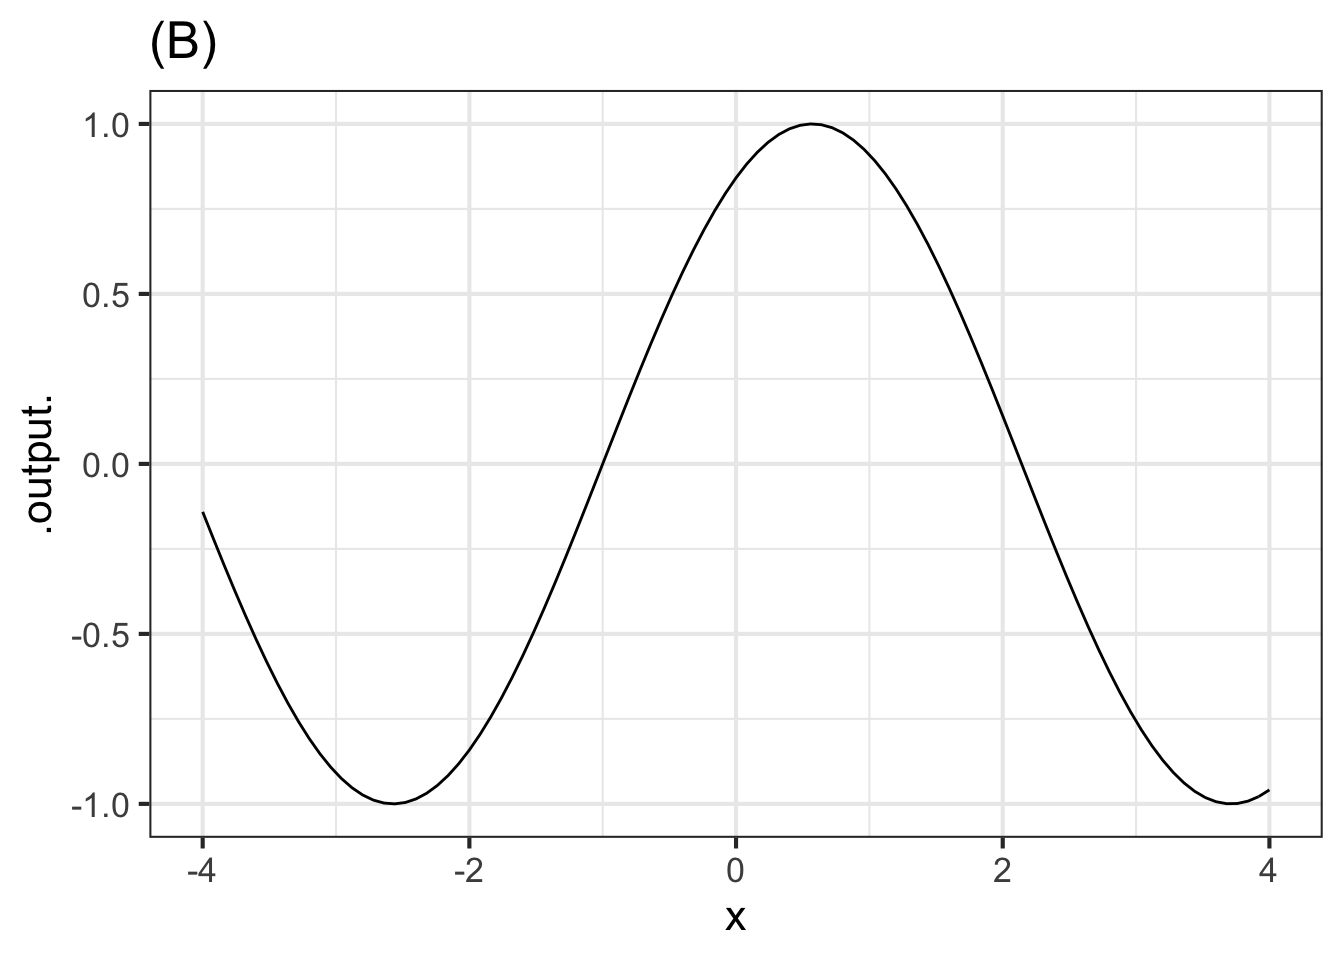
\includegraphics{Preliminaries/exercise-layout_files/figure-pdf/unnamed-chunk-21-1.pdf}

}

\end{figure}

In this exercise, you'll be modifying the sandbox code to draw different
functions, so you can examine their shapes.

Your task is to read and interpret the graphs of the basic modeling
functions. Here, you will be looking for \textbf{\emph{zero-crossings}}:
the neighborhood of a point in the function's domain where the
\textbf{output} of the function is negative for inputs on one side and
positive for inputs on the other side. If zero is touched but not
crossed, we'll call that ``touched zero.''

Make a list of the pattern-book functions. For each function in the
list, say whether the function crosses zero, touches zero but doesn't
cross, or doesn't touch at all in the part of the domain shown in the
graphic: \(-3 \leq x \leq 3\). Also note if the value of the function
appears to be reaching a horizontal asymptote at zero for very negative
\(x\), for very positive \(x\), for both, or neither.

We'll show you the answers for the exponential function. You'll have to
modify the computer command to graph the other pattern-book functions.

\begin{figure*}

\begin{longtable}[]{@{}
  >{\raggedright\arraybackslash}p{(\columnwidth - 6\tabcolsep) * \real{0.1972}}
  >{\raggedright\arraybackslash}p{(\columnwidth - 6\tabcolsep) * \real{0.1690}}
  >{\raggedright\arraybackslash}p{(\columnwidth - 6\tabcolsep) * \real{0.4366}}
  >{\raggedright\arraybackslash}p{(\columnwidth - 6\tabcolsep) * \real{0.1972}}@{}}
\toprule()
\begin{minipage}[b]{\linewidth}\raggedright
function name
\end{minipage} & \begin{minipage}[b]{\linewidth}\raggedright
R formula
\end{minipage} & \begin{minipage}[b]{\linewidth}\raggedright
zero in domain shown in graph
\end{minipage} & \begin{minipage}[b]{\linewidth}\raggedright
asymptotic zero
\end{minipage} \\
\midrule()
\endhead
exponential & \texttt{exp(x)} & no zeros & for very negative \(x\) \\
logarithm & & & \\
sinusoid & & & \\
square & & & \\
proportional & & & \\
constant & & & \\
reciprocal & & & \\
gaussian & & & \\
sigmoid & & & \\
\bottomrule()
\end{longtable}

\end{figure*}

\hypertarget{exer.-5.2}{%
\section*{Exer. 5.2}\label{exer.-5.2}}
\addcontentsline{toc}{section}{Exer. 5.2}

\textbf{Exercise 5.2}
../Preliminaries/Exercises/lobster-ride-glasses.Rmd

On a piece of paper, sketch from memory a graph of each of the nine
pattern-book functions.

\hypertarget{exer.-5.3}{%
\section*{Exer. 5.3}\label{exer.-5.3}}
\addcontentsline{toc}{section}{Exer. 5.3}

\textbf{Exercise 5.3}
../Preliminaries/Exercises/pattern-book-axis-crossing.Rmd

For each of the pattern-book functions except the reciprocal, the graph
crosses either the vertical axis (that is \(x=0\)) or the horizontal
axis (that is, \(f(x) = 0\)), or both. It's helpful to know the exact
quantitative value for the output where the function graph crosses the
vertical axis.

To answer these questions, you will want to open a SANDBOX to try the
various possibilities.

\textbf{Question A} What is the exact output of the pattern-book
\textbf{exponential} function when the input is \(x=0\)?

~~~~{0{x}}~~~~~~~{0.3989423{x}}~~~~~~~{1/2{︎X
}}~~~~~~~{1{\(\heartsuit\ \)}}

\textbf{Question B} What is the exact output of the pattern-book
\textbf{sine} function when the input is \(x=0\)?

~~~~{0{\(\heartsuit\ \)}}~~~~~~~{0.3989423{x}}~~~~~~~{1/2{︎X
}}~~~~~~~{1{x}}

\textbf{Question C} What is the exact output of the pattern-book
\textbf{sigmoid} function when the input is \(x=0\)?

~~~~{0{x}}~~~~~~~{0.3989423{︎X
}}~~~~~~~{1/2{\(\heartsuit\ \)}}~~~~~~~{1{x}}

\textbf{Question D} What is the output (to several digits) of the
pattern-book \textbf{hump} function when the input is \(x=0\)?

~~~~{0{x}}~~~~~~~{0.3989423{\(\heartsuit\ \)Right. But 0.4 will do
when you're sketching a graph.}}~~~~~~~{1/2{x}}~~~~~~~{1{x}}

\textbf{Question E} What is the exact output of the pattern-book
\textbf{constant} function?

~~~~{0{x}}~~~~~~~{0.3989423{x}}~~~~~~~{1/2{︎X
}}~~~~~~~{1{\(\heartsuit\ \)}}

\hypertarget{exer.-5.4}{%
\section*{Exer. 5.4}\label{exer.-5.4}}
\addcontentsline{toc}{section}{Exer. 5.4}

\textbf{Exercise 5.4} ../Preliminaries/Exercises/cat-lend-futon.Rmd

\textbf{Question A} True or false: \(2^x\) is a power-law function.

\begin{enumerate}
\def\labelenumi{\roman{enumi}.}
\tightlist
\item
  {TRUE{xIn a power-law function, the input is the base. In \(2^x\),
  the input is the exponent. So it's an exponential function.}}\\
\item
  {FALSE{Correct.~}}
\end{enumerate}

\textbf{Question B} True or false: \(3/x^2\) is a power-law function.

\begin{enumerate}
\def\labelenumi{\roman{enumi}.}
\tightlist
\item
  {TRUE{Right!~}}\\
\item
  {FALSE{xThis is the same as \(3 x^{-2}\). You can see that \(x\) is
  the base, so this is a power-law function.}}
\end{enumerate}

\textbf{Question C} True or false: \(5\sqrt{x}\) is a power-law
function.

\begin{enumerate}
\def\labelenumi{\roman{enumi}.}
\tightlist
\item
  {TRUE{Correct.~}}\\
\item
  {FALSE{xThis is the same as \(5 x^{1/2}\). The input \(x\) is the
  base, so this is a power-law function.}}
\end{enumerate}

\textbf{Question D} The gravitational force, F, between two bodies is
inversely proportional to the square of the distance \(d\) between them.
Then \ldots{}

\begin{enumerate}
\def\labelenumi{\roman{enumi}.}
\tightlist
\item
  {\(F = k d^{2}\){xInversely proportional to the square would be
  \(d^{-2}\)}}\\
\item
  {\(F = kd^{-2}\){Correct.~}}\\
\item
  {\(F = k d^{1/2}\){xThis is a square-root relationship.}}\\
\item
  {\(F = k d^{-1/2}\){xThis is inversely proportional to the square
  root.}}
\end{enumerate}

\hypertarget{exer.-5.5}{%
\section*{Exer. 5.5}\label{exer.-5.5}}
\addcontentsline{toc}{section}{Exer. 5.5}

\textbf{Exercise 5.5} ../Preliminaries/Exercises/bear-lay-plant.Rmd

Some of our pattern-book functions have a distinctive property called
\textbf{scale invariance}. This means the graph of the function looks
the same even when plotted on very different horizontal and vertical
axes. The function \(\ln(x)\) plotted on two different scales in Figure
@ref(fig:log-scale-invariance) shows that the graph of the function has
practically the same shape.

\begin{figure}

{\centering 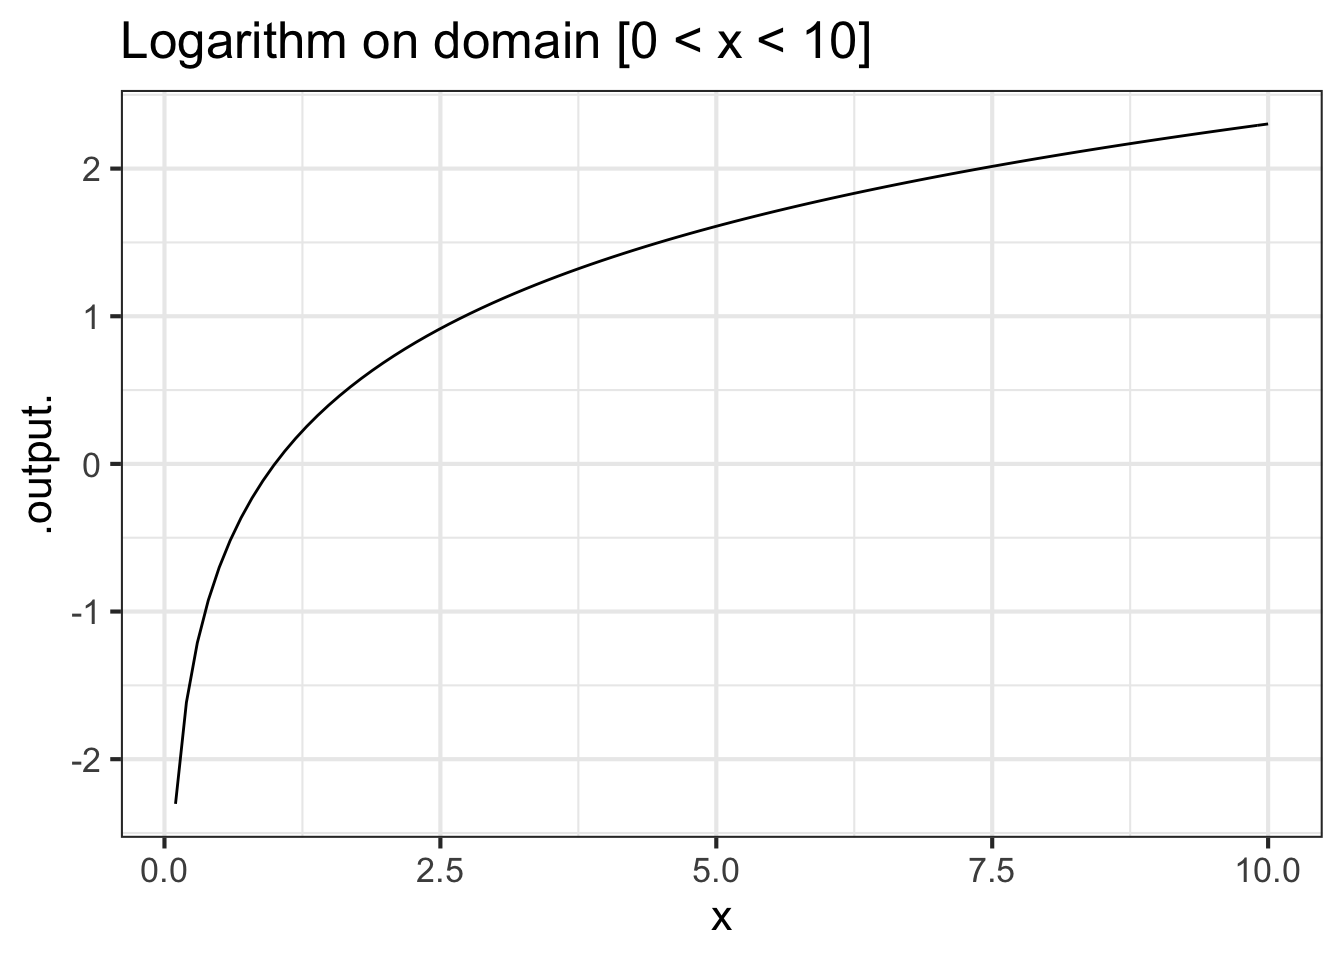
\includegraphics[width=0.5\textwidth,height=\textheight]{Preliminaries/exercise-layout_files/figure-pdf/fig-log-scale-invariance-1.pdf}

}

\caption{\label{fig-log-scale-invariance-1}The logarithm function has
the same overall shape even when plotted on domains of very different
scales.}

\end{figure}

\begin{figure}

{\centering 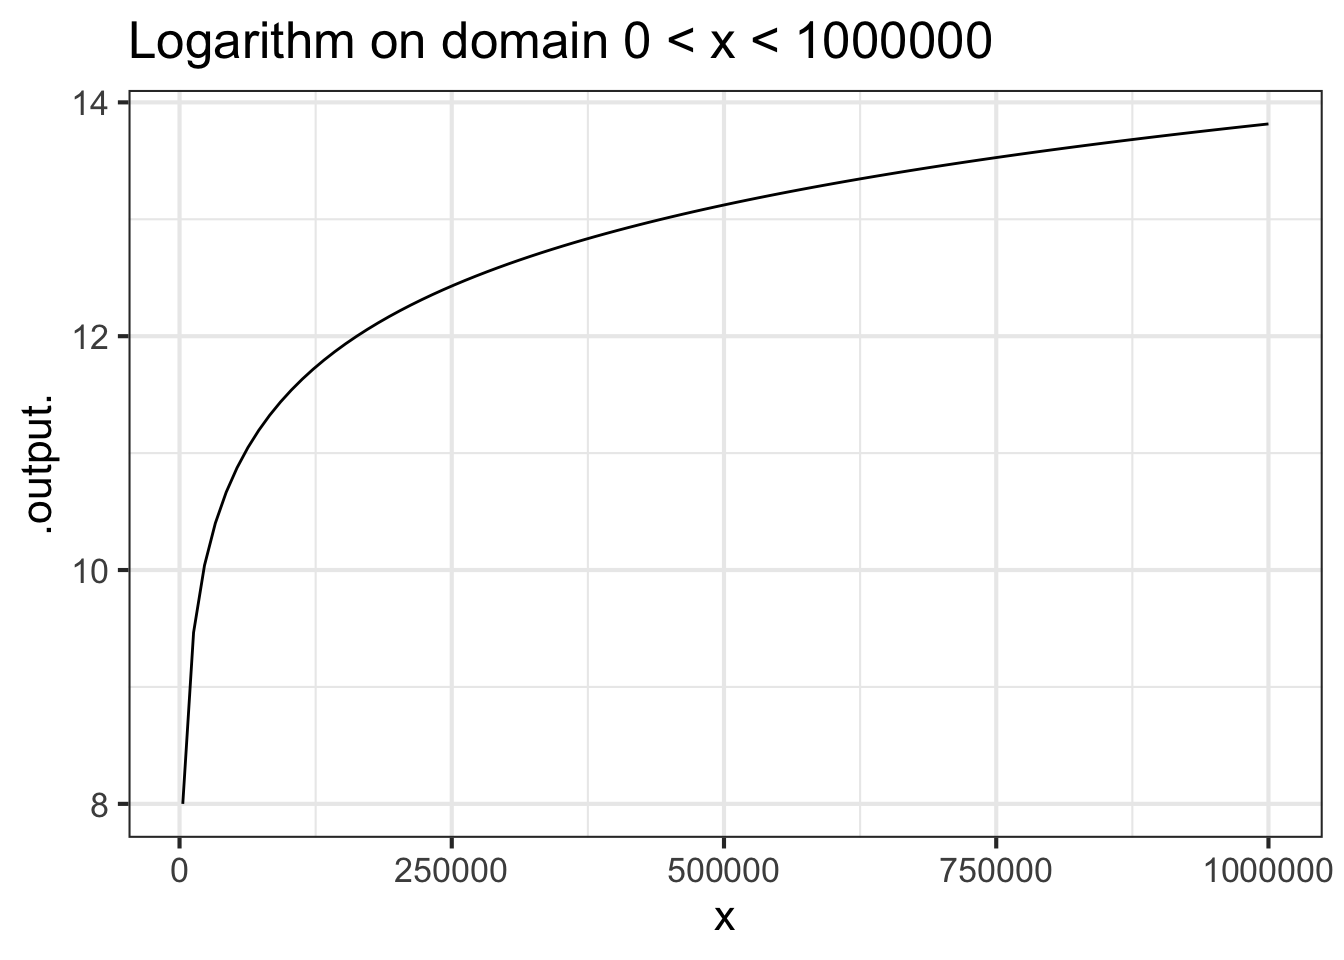
\includegraphics[width=0.5\textwidth,height=\textheight]{Preliminaries/exercise-layout_files/figure-pdf/fig-log-scale-invariance-2.pdf}

}

\caption{\label{fig-log-scale-invariance-2}The logarithm function has
the same overall shape even when plotted on domains of very different
scales.}

\end{figure}

Figure @ref(fig:square-invariance) shows a power-law function,
\(g(x) \equiv x^2\), which is also scale invariant.

\begin{figure}

{\centering 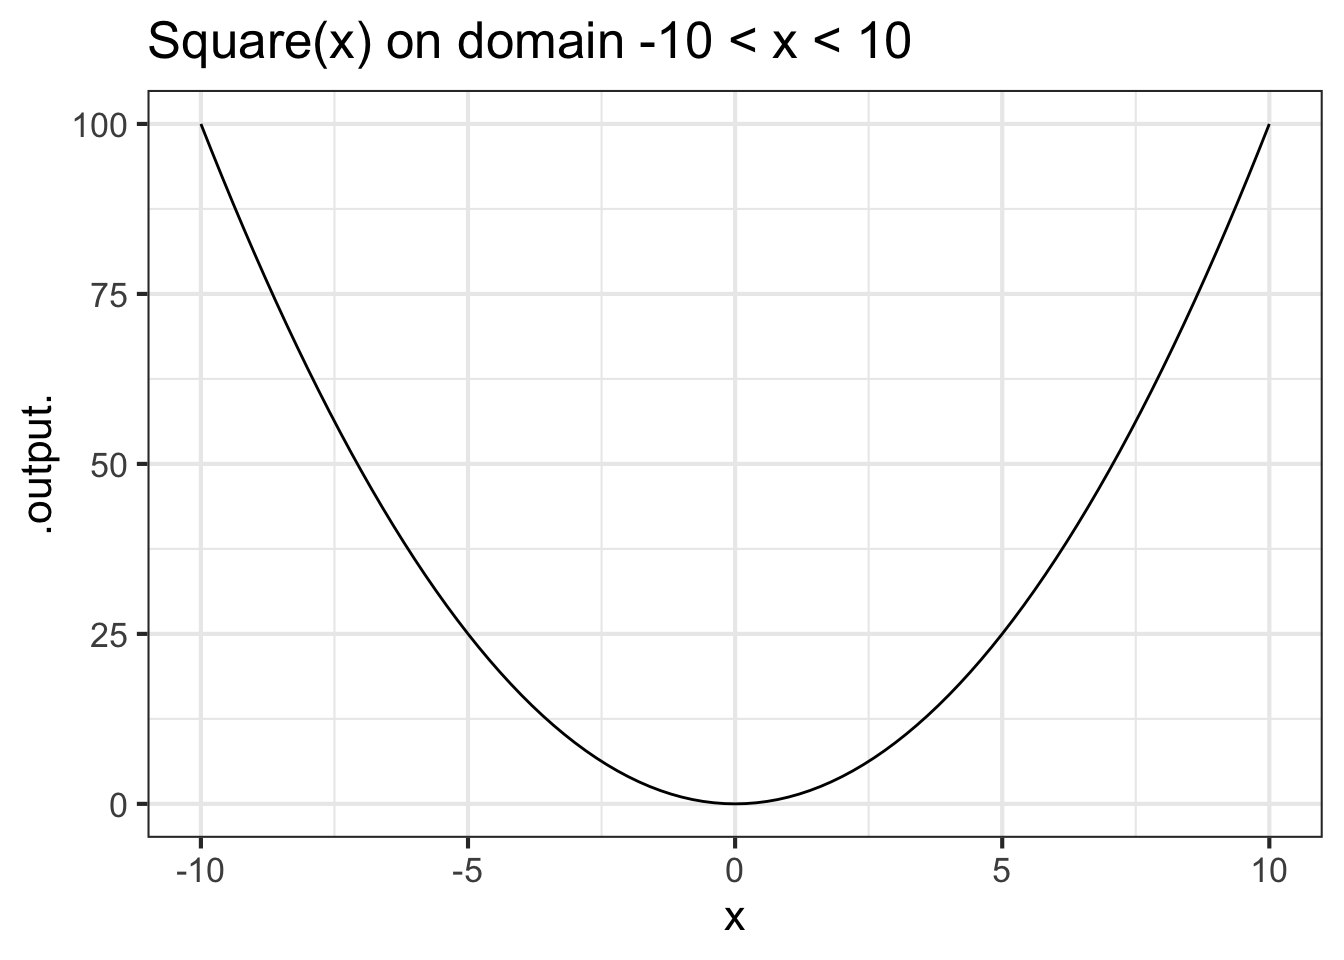
\includegraphics[width=0.5\textwidth,height=\textheight]{Preliminaries/exercise-layout_files/figure-pdf/fig-square-invariance-1.pdf}

}

\caption{\label{fig-square-invariance-1}The function \(x^2\) shown on
two very different domain scales has the same overall shape.}

\end{figure}

\begin{figure}

{\centering 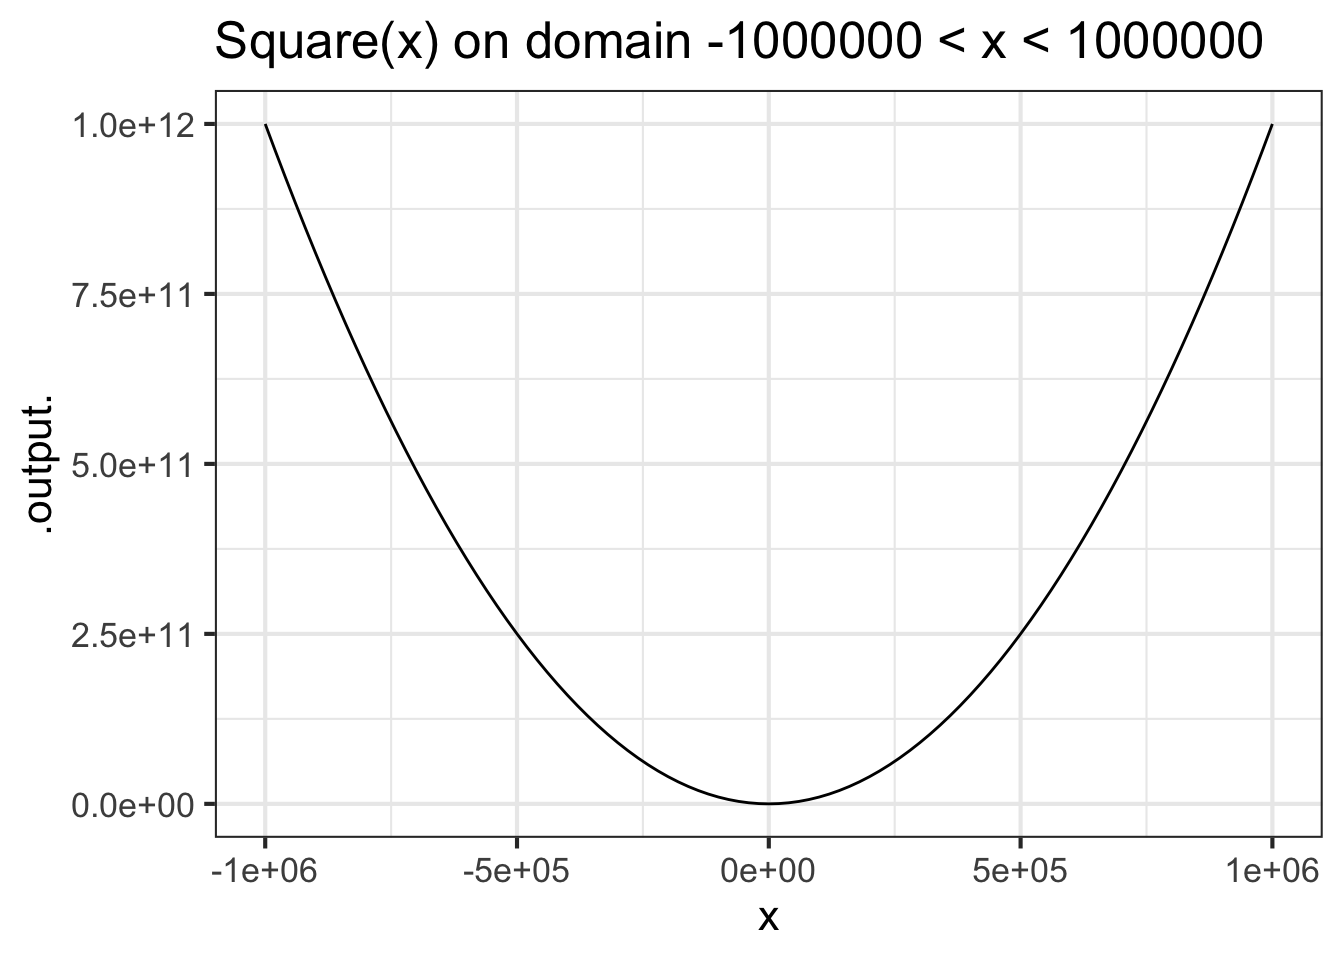
\includegraphics[width=0.5\textwidth,height=\textheight]{Preliminaries/exercise-layout_files/figure-pdf/fig-square-invariance-2.pdf}

}

\caption{\label{fig-square-invariance-2}The function \(x^2\) shown on
two very different domain scales has the same overall shape.}

\end{figure}

Other pattern-book functions are not scale invariant, for example
\(\sin(x)\).

\begin{figure}

{\centering 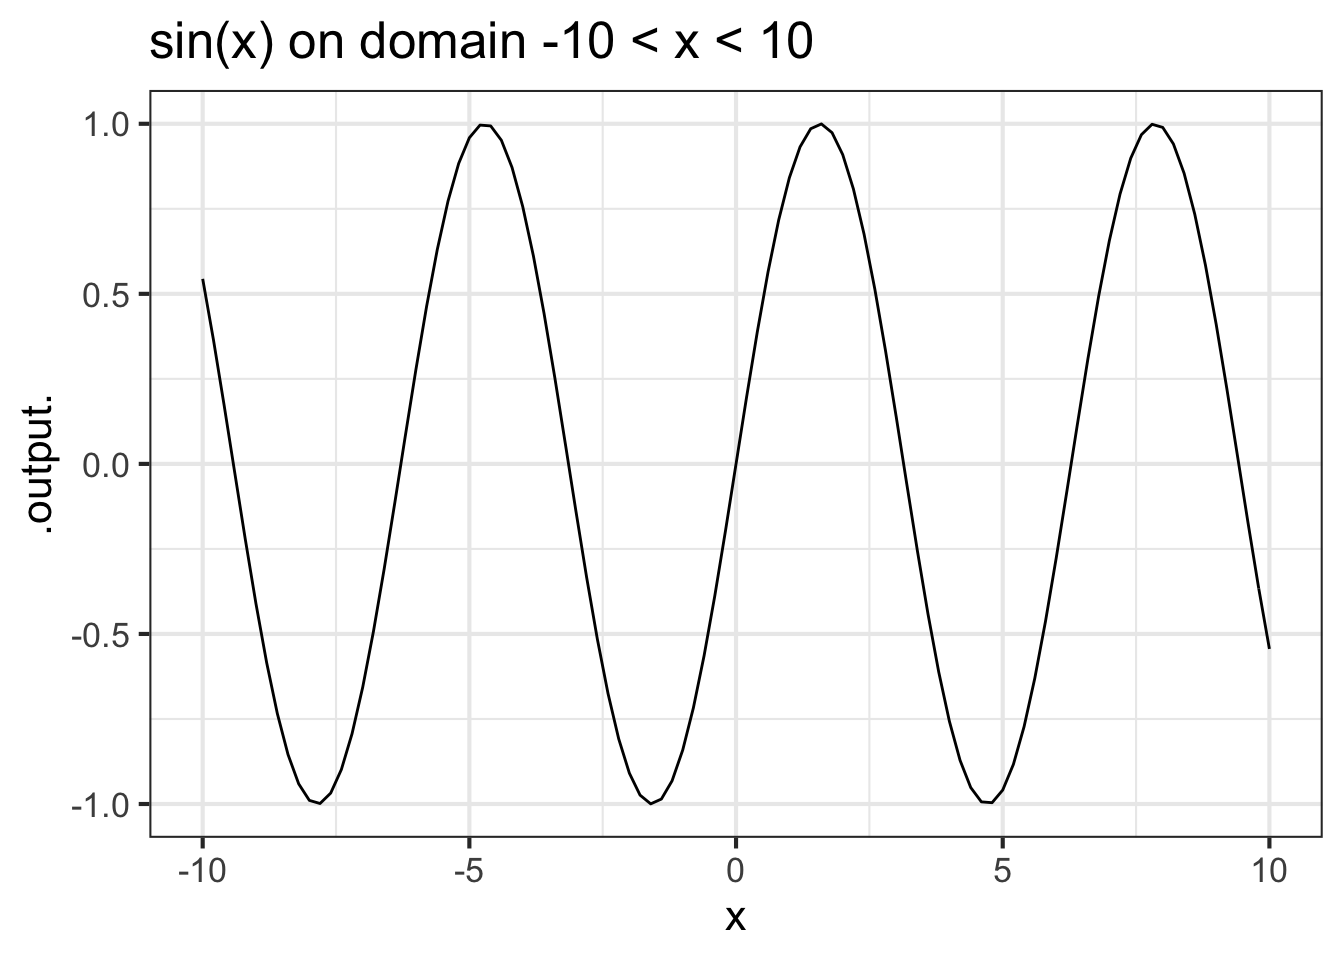
\includegraphics[width=0.5\textwidth,height=\textheight]{Preliminaries/exercise-layout_files/figure-pdf/fig-sin-invariance-1.pdf}

}

\caption{\label{fig-sin-invariance-1}The sin( ) function is not scale
invariant.}

\end{figure}

\begin{figure}

{\centering 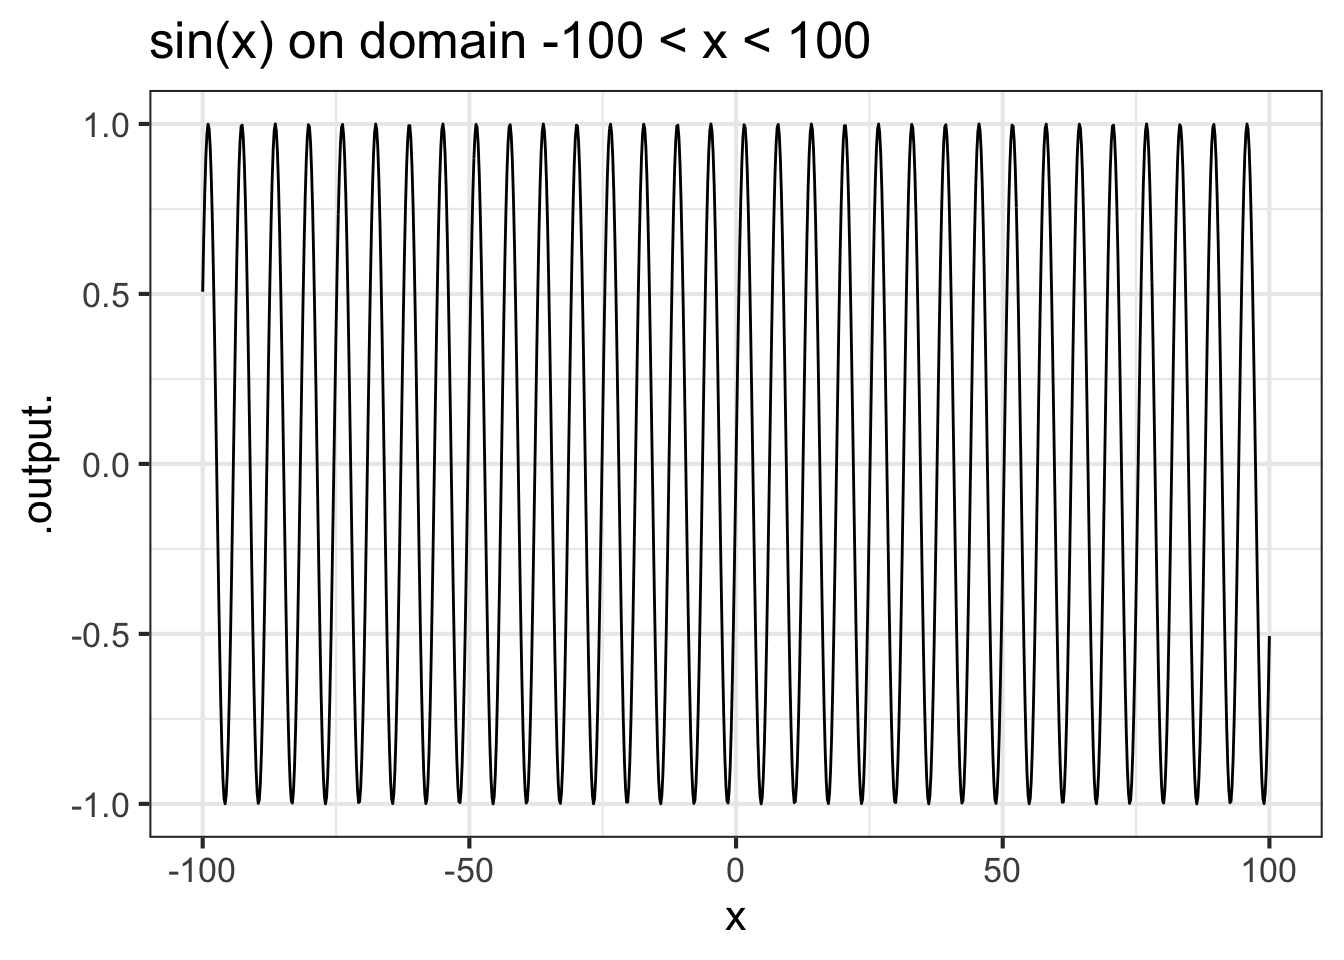
\includegraphics[width=0.5\textwidth,height=\textheight]{Preliminaries/exercise-layout_files/figure-pdf/fig-sin-invariance-2.pdf}

}

\caption{\label{fig-sin-invariance-2}The sin( ) function is not scale
invariant.}

\end{figure}

In contrast to scale-invariant functions, some of our pattern-book
functions have a \textbf{\emph{characteristic scale}}. This is a domain
length over which the whole of a characteristic feature of the function
is evident. Graphing on larger domains simply squashes down the
characteristic feature to a small part of the graphic domain. For
instance, in the \(\sin()\) function the cycle is a characteristic
feature. The cycle in the pattern-book sinusoid has a characteristic
length of \(2 \pi\), the length of the cycle. Consequently, the graph
looks different depending on the length of the graphics domain in
multiples of the characteristic length. You can see from Figure
@ref(fig:sin-invariance) that the graph on the domain \(-10 < x < 10\),
that is, about 3 times the characteristic scale, looks different from
the graph on the larger domain that has a length 30 times the
characteristic scale.

The output of the sigmoid function runs from 0 to 1 but reaches these
values only asymptotically, as \(x \rightarrow \pm \infty\). In defining
a characteristic scale, it would be reasonable to look at the length of
the domain that takes the output from, say, 0.01 to 0.99. In other
words, we want the characteristic scale to be defined in a way that
captures \textbf{almost} all the action in the output of the function.
For a gaussian, a reasonable definition of a characteristic scale would
be the length of domain where the output falls to about, say, 1\% of
it's peak output.

\textbf{Question A} The gaussian (hump) function \texttt{dnorm()} has a
characteristic scale. Which of these is a domain length that can
encompass the characteristic shape of the gaussian?

~~~~{0.1{x}}~~~~~~~{1{x}}~~~~~~~{6{\(\heartsuit\ \)The domain
\(-3 < x < 3\) supports practically everything.}}~~~~~~~{16{︎X
}}~~~~~~~{256{x}}

\textbf{Question B} The sigmoid function \texttt{pnorm()} also has a
characteristic scale. Which of these is a domain length that can
encompass the characteristic shape of the sigmoid?

~~~~{0.1{x}}~~~~~~~{1{x}}~~~~~~~{6{\(\heartsuit\ \)}}~~~~~~~{16{︎X
}}~~~~~~~{256{x}}

Throughout science, it's common to set a standard approach to defining a
characteristic scale. For instance, the characteristic scale of an
aircraft could be taken as the length of body. Gaussian and sigmoids are
so common throughout science that there is a convention for defining the
characteristic scale called the \textbf{\emph{standard deviation}}. For
the pattern book gaussian and sigmoid, the standard deviation is 1.
That's much shorter than the domain that captures the bulk of action of
the gaussian or sigmoid. For this reason, statisticians in practice use
a characteristic scale of \(\pm 2\) or \(\pm 3\) standard deviations.

\hypertarget{exer.-5.6}{%
\section*{Exer. 5.6}\label{exer.-5.6}}
\addcontentsline{toc}{section}{Exer. 5.6}

\textbf{Exercise 5.6} ../Preliminaries/Exercises/pattern-book-domain.Rmd

All but two of the pattern-book functions have a domain that runs over
the whole number line: \(-\infty < x < \infty\).

Which pattern-book function has a domain that excludes zero and negative
numbers as inputs?

Which pattern-book function has just a single value missing from its
domain?

\hypertarget{exer.-5.7}{%
\section*{Exer. 5.7}\label{exer.-5.7}}
\addcontentsline{toc}{section}{Exer. 5.7}

\textbf{Exercise 5.7} ../Preliminaries/Exercises/range-domain.Rmd

Consider this graph of a function \(g(x)\):

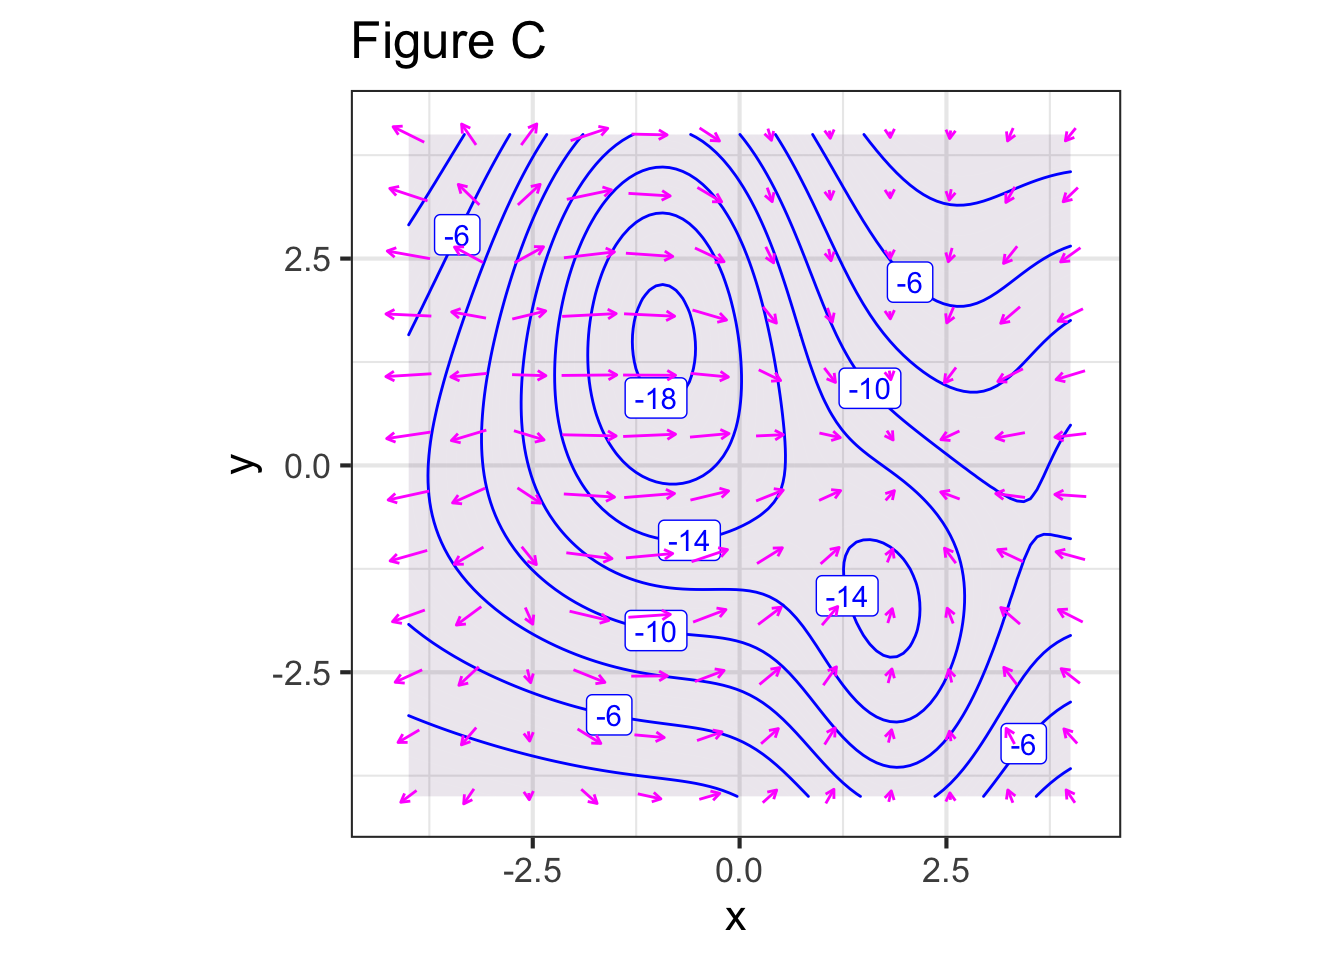
\includegraphics{Preliminaries/exercise-layout_files/figure-pdf/unnamed-chunk-30-1.pdf}

\textbf{Question A} What is the \textbf{domain} of \(g(x)\)?

\begin{enumerate}
\def\labelenumi{\roman{enumi}.}
\tightlist
\item
  {\(-\infty < x < \infty\){x}}\\
\item
  {\(-3 \leq x \leq 2\){Correct.~}}\\
\item
  {\(-4 \leq x \leq 4\){xThis might be called the ``graphics'' domain,
  yet the function graph doesn't extend over that whole interval.}}\\
\item
  {\(-10 \leq g(x) \leq 40\){xThis is the vertical extent of the
  \textbf{graphics frame}.}}\\
\item
  {\(-1 \leq g(x) \leq 33\){xThe \textbf{domain} refers to the
  horizontal axis.}}
\end{enumerate}

\textbf{Question B} What is the \textbf{range} of \(g(x)\)?

\begin{enumerate}
\def\labelenumi{\roman{enumi}.}
\tightlist
\item
  {\(-\infty < x < \infty\){xThe \textbf{range} refers output of the
  function. \(x\) is the input.}}\\
\item
  {\(-3 \leq x \leq 2\){xThe \textbf{range} refers output of the
  function. \(x\) is the input.}}\\
\item
  {\(-4 \leq y \leq 4\){xYou're used to calling the function output
  \(y\), but that's a bad habit. Break it!}}\\
\item
  {\(-10 \leq g(x) \leq 40\){xThis is the vertical extent of the
  \textbf{graphics frame}.}}\\
\item
  {\(-1 \leq g(x) \leq 33\){Good.~}}
\end{enumerate}

\hypertarget{exer.-5.8}{%
\section*{Exer. 5.8}\label{exer.-5.8}}
\addcontentsline{toc}{section}{Exer. 5.8}

\textbf{Exercise 5.8} ../Preliminaries/Exercises/pattern-book-range.Rmd

A function's \textbf{\emph{domain}} is the set of possible inputs to the
function. A function's \textbf{\emph{range}} is the set of possible
outputs. For each of the pattern-book functions, specify what is the
range.

\textbf{Question A} What is the range of the pattern-book
\textbf{exponential} function?

\begin{enumerate}
\def\labelenumi{\roman{enumi}.}
\tightlist
\item
  {All positive outputs{Nice!~}}\\
\item
  {All negative outputs{x}}\\
\item
  {The whole number line{x}}\\
\item
  {A closed, finite interval of possibilities{x}}
\end{enumerate}

\textbf{Question B} What is the range of the pattern-book \textbf{sine}
function?

\begin{enumerate}
\def\labelenumi{\roman{enumi}.}
\tightlist
\item
  {All positive outputs{x}}\\
\item
  {All negative outputs{x}}\\
\item
  {The whole number line{x}}\\
\item
  {A closed, finite interval of possibilities{Excellent!~Yes. The output
  of pattern-book sinusoid functions is always in the interval from -1
  to 1, inclusive}}
\end{enumerate}

\textbf{Question C} What is the range of the pattern-book
\textbf{logarithm} function?

\begin{enumerate}
\def\labelenumi{\roman{enumi}.}
\tightlist
\item
  {All positive outputs{x}}\\
\item
  {All non-negative outputs{x}}\\
\item
  {All negative outputs{x}}\\
\item
  {The whole number line{Correct.~}}\\
\item
  {A closed, finite interval of possibilities{x}}
\end{enumerate}

\textbf{Question D} What is the range of the pattern-book
\textbf{square} function?

\begin{enumerate}
\def\labelenumi{\roman{enumi}.}
\tightlist
\item
  {All positive outputs{xClose. Zero is one of the possible outputs.
  We can say, equivalently, that the range is all the \textbf{positive
  outputs plus 0} or all the \textbf{non-negative} outputs.}}\\
\item
  {All non-negative outputs{Nice!~}}\\
\item
  {All negative outputs{x}}\\
\item
  {The whole number line{x}}\\
\item
  {A closed, finite interval of possibilities{x}}
\end{enumerate}

\textbf{Question E} What is the range of the pattern-book
\textbf{proportional} function?

\begin{enumerate}
\def\labelenumi{\roman{enumi}.}
\tightlist
\item
  {All positive outputs{x}}\\
\item
  {All negative outputs{x}}\\
\item
  {The whole number line{Correct.~}}\\
\item
  {A closed, finite interval of possibilities{xThe range extends from
  \(-\infty\) to \(\infty\).}}
\end{enumerate}

\textbf{Question F} What is the range of the pattern-book
\textbf{sigmoid} function?

\begin{enumerate}
\def\labelenumi{\roman{enumi}.}
\tightlist
\item
  {All positive outputs{x}}\\
\item
  {All negative outputs{x}}\\
\item
  {The whole number line{x}}\\
\item
  {A closed, finite interval of possibilities{Correct.~Right. The
  pattern-book sigmoid function has an output that is always in the
  interval \(0 \leq \pnorm(x) \leq 1 .\)}}
\end{enumerate}

\hypertarget{exer.-6.1}{%
\section*{Exer. 6.1}\label{exer.-6.1}}
\addcontentsline{toc}{section}{Exer. 6.1}

\textbf{Exercise 6.1}
../Preliminaries/Exercises/pattern-book-descriptions.Rmd

Answer these questions about the pattern-book functions. You can refer
to the graphs in Figures @ref(fig:monomial-graphs) through
@ref(fig:non-integer-graphs).

\textbf{Question A} Which of these best describes the concavity of the
gaussian function?

\begin{enumerate}
\def\labelenumi{\roman{enumi}.}
\tightlist
\item
  {It's not concave.{xIf it curves, it's either concave up or
  down.}}\\
\item
  {It's concave down.{xIn some places, but not in others.}}\\
\item
  {It's concave down in the center and concave up on both
  flanks.{Good.~}}\\
\item
  {It's concave down on the left and concave up on the right{xLook
  again}}
\end{enumerate}

\textbf{Question B} Which of these best describes the concavity of the
sigmoid function?

\begin{enumerate}
\def\labelenumi{\roman{enumi}.}
\tightlist
\item
  {It's not concave.{xIf it curves, it's either concave up or
  down.}}\\
\item
  {It's concave down.{xIn some places, but not in others.}}\\
\item
  {It's concave down on the left and concave up on the right.{xLook
  again}}\\
\item
  {It's concave up on the left and concave down on the right.{Nice!~}}
\end{enumerate}

\textbf{Question C} Which of these best describes the concavity of the
second-order monomial \(m_2(x) \equiv x^2\)?

\begin{enumerate}
\def\labelenumi{\roman{enumi}.}
\tightlist
\item
  {It's not concave.{xIf it curves, it's either concave up or
  down.}}\\
\item
  {It's concave down.{xIs it a smile or a frown?}}\\
\item
  {It's concave down on the left and concave up on the right.{xLook
  again}}\\
\item
  {It's concave up everywhere.{Excellent!~}}
\end{enumerate}

\hypertarget{exer.-6.2}{%
\section*{Exer. 6.2}\label{exer.-6.2}}
\addcontentsline{toc}{section}{Exer. 6.2}

\textbf{Exercise 6.2}
../Preliminaries/Exercises/pattern-book-concave.Rmd

In this activity, you will be examining the various pattern-book
functions to look for two different features:

\begin{enumerate}
\def\labelenumi{\arabic{enumi}.}
\tightlist
\item
  \textbf{\emph{Slope}}: whether the graph has a slope that is
  consistently positive, negative, both, or neither, and
\item
  \textbf{\emph{Concavity}}: whether the function being graphed is
  concave up, concave down, neither, or both (i.e., concave up in some
  regions of the domain and down for others).
\end{enumerate}

\begin{scaffolding}

Copy and paste the R/mosaic command below in a SANDBOX to draw a
function graph. Remember to press ``Run code.'' ::: \{.cell\}

\begin{Shaded}
\begin{Highlighting}[]
\FunctionTok{slice\_plot}\NormalTok{(}\FunctionTok{exp}\NormalTok{(x) }\SpecialCharTok{\textasciitilde{}}\NormalTok{ x, }\FunctionTok{domain}\NormalTok{(}\AttributeTok{x=}\FunctionTok{c}\NormalTok{(}\SpecialCharTok{{-}}\DecValTok{3}\NormalTok{, }\DecValTok{3}\NormalTok{)))}
\end{Highlighting}
\end{Shaded}

\begin{figure}[H]

{\centering 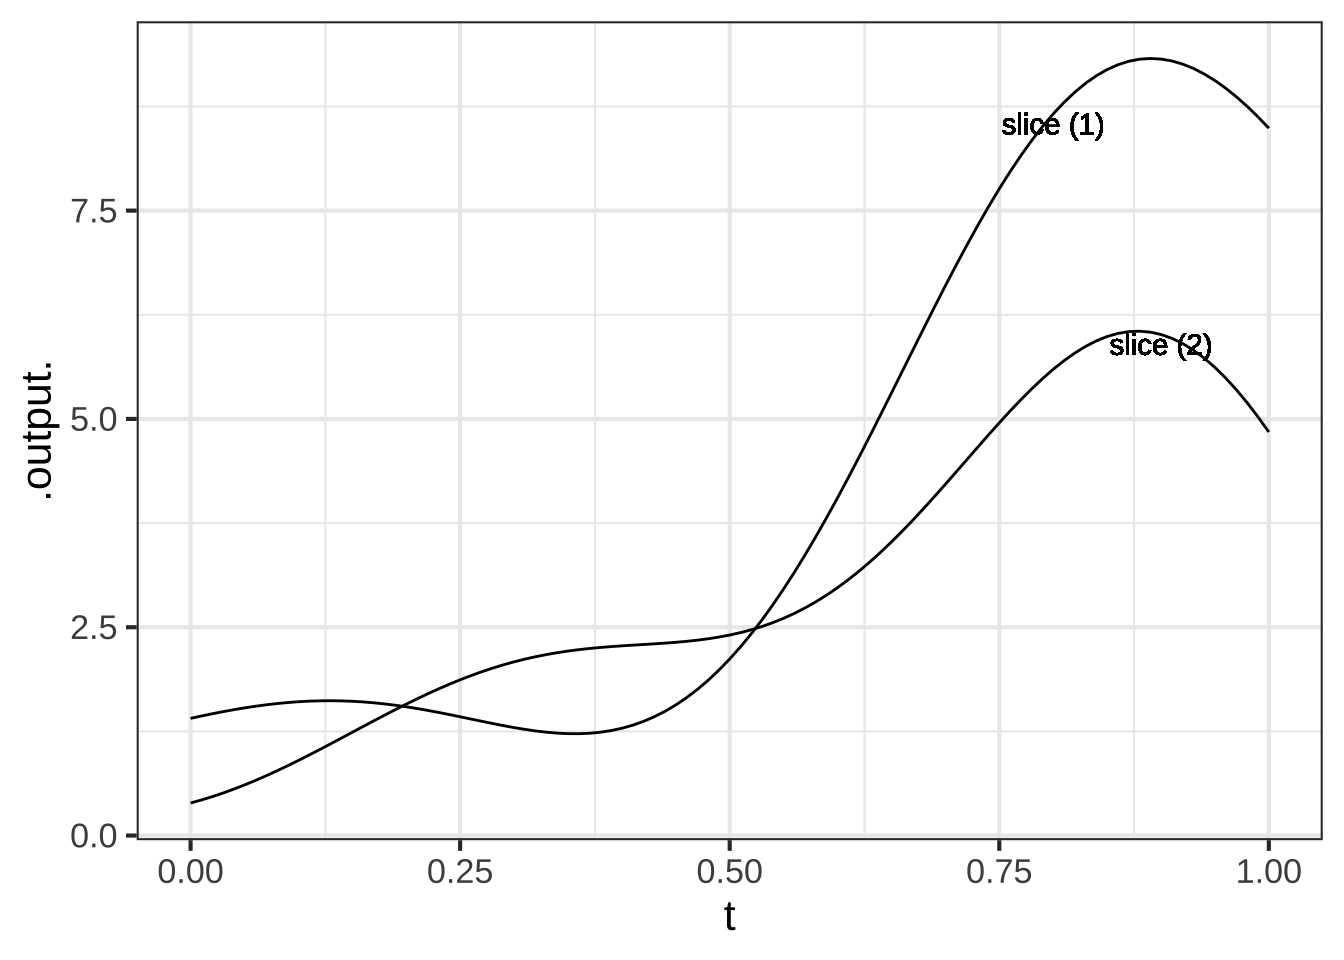
\includegraphics{Preliminaries/exercise-layout_files/figure-pdf/unnamed-chunk-34-1.pdf}

}

\end{figure}

\end{scaffolding}

To modify the command to draw another function, replace the
\texttt{exp(x)} with another formula, for instance \texttt{1/x}.

:::

Make a list of the pattern-book functions. For each function in the
list, write down the R expression for the function, say whether the
function has a consistently positive or negative slope, whether it is
consistently concave up or down, and if the value of the function
appears to be reaching a horizontal asymptote at zero for very negative
\(x\), for very positive \(x\), for both, or neither.

We'll show you the answers for the exponential and sinusoid functions.
You'll have to modify the computer command to graph the other
pattern-book functions.

\begin{longtable}[]{@{}
  >{\raggedright\arraybackslash}p{(\columnwidth - 8\tabcolsep) * \real{0.2222}}
  >{\raggedright\arraybackslash}p{(\columnwidth - 8\tabcolsep) * \real{0.1905}}
  >{\raggedright\arraybackslash}p{(\columnwidth - 8\tabcolsep) * \real{0.2381}}
  >{\raggedright\arraybackslash}p{(\columnwidth - 8\tabcolsep) * \real{0.2222}}
  >{\raggedright\arraybackslash}p{(\columnwidth - 8\tabcolsep) * \real{0.1270}}@{}}
\toprule()
\begin{minipage}[b]{\linewidth}\raggedright
function name
\end{minipage} & \begin{minipage}[b]{\linewidth}\raggedright
R formula
\end{minipage} & \begin{minipage}[b]{\linewidth}\raggedright
slope
\end{minipage} & \begin{minipage}[b]{\linewidth}\raggedright
concavity
\end{minipage} & \begin{minipage}[b]{\linewidth}\raggedright
horiz. asymptote
\end{minipage} \\
\midrule()
\endhead
exponential & \texttt{exp(x)} & positive & concave up &
\(x \rightarrow -\infty\) \\
logarithm & & & & \\
sinusoid & \texttt{sin(x)} & both & both & neither \\
square & & & & \\
proportional & & & & \\
constant & & & & \\
reciprocal & & & & \\
gaussian & & & & \\
sigmoid & & & & \\
\bottomrule()
\end{longtable}

\hypertarget{exer.-8.2}{%
\section*{Exer. 8.2}\label{exer.-8.2}}
\addcontentsline{toc}{section}{Exer. 8.2}

\textbf{Exercise 8.2} ../Modeling/Exercises/scale-input-1.Rmd

Each of the graphs shows two horizontal scales and one of the basic
modeling functions. Which horizontal scale (black or blue) corresponds
to the pattern-book function?

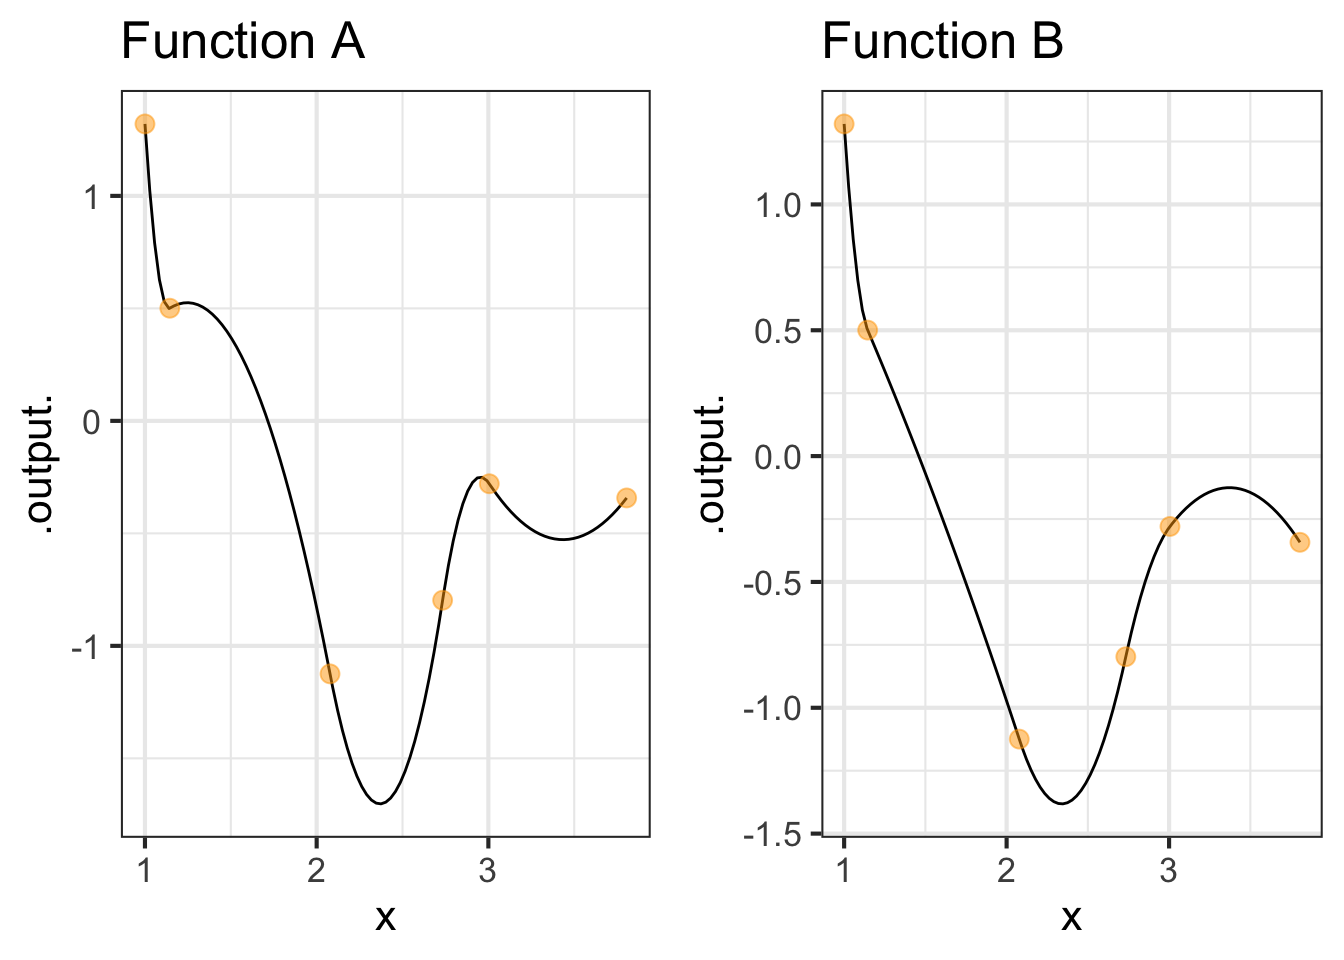
\includegraphics{Preliminaries/exercise-layout_files/figure-pdf/unnamed-chunk-38-1.pdf}

\textbf{Question A} For graph (A), which scale corresponds to the
pattern-book function?

\begin{enumerate}
\def\labelenumi{\roman{enumi}.}
\tightlist
\item
  {black{Correct.~}}\\
\item
  {blue{x}}\\
\item
  {neither{x}}\\
\item
  {both{xIt can't be both. There's only one pattern-book function.
  When you scale the input, it becomes a ``basic modeling function''.}}
\end{enumerate}

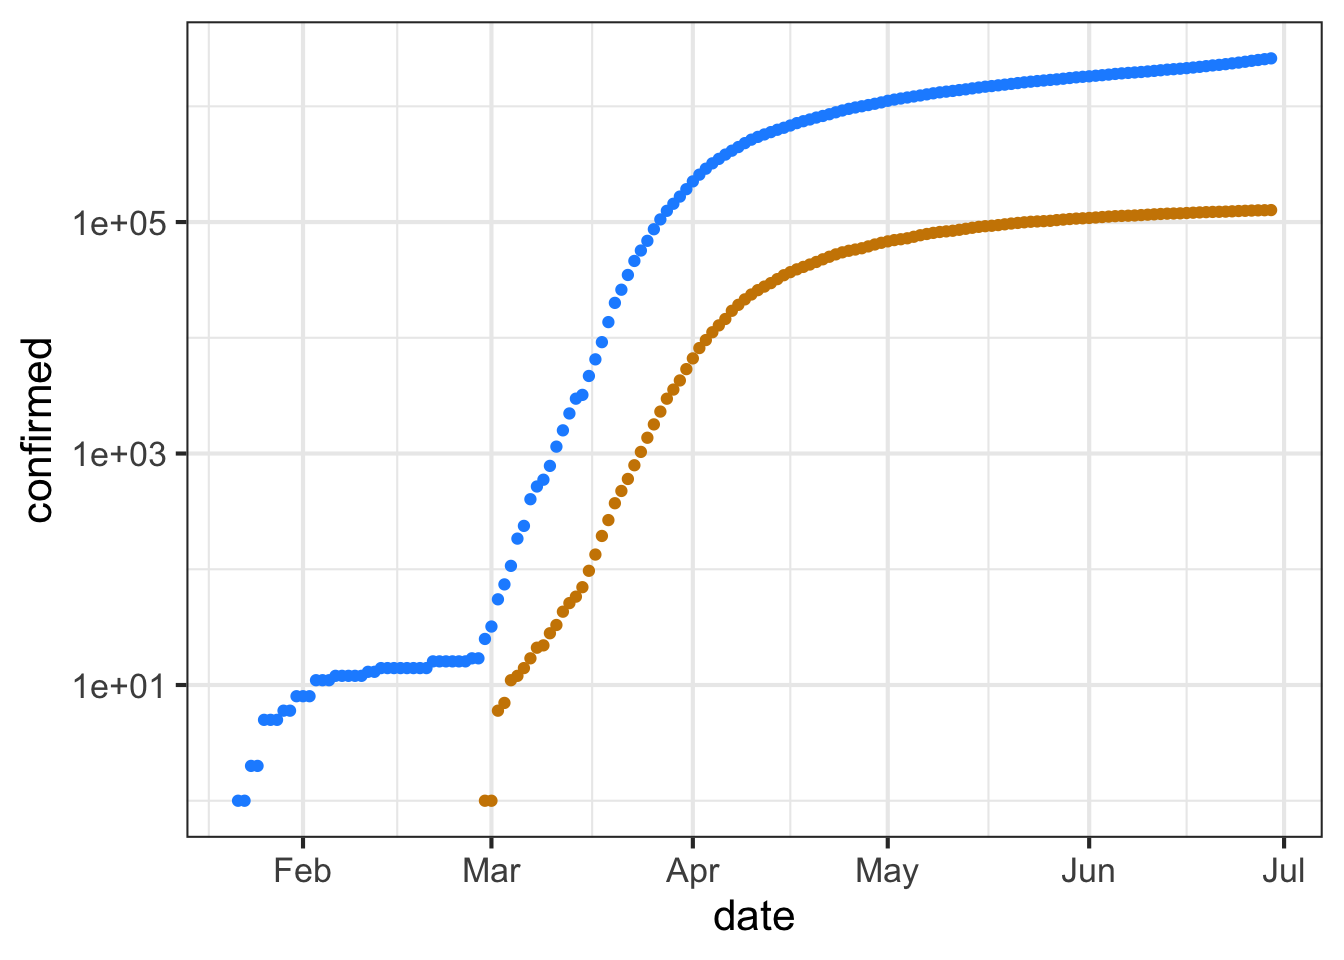
\includegraphics{Preliminaries/exercise-layout_files/figure-pdf/unnamed-chunk-40-1.pdf}

\textbf{Question B} For graph (B), which scale corresponds to the
pattern-book function?

\begin{enumerate}
\def\labelenumi{\roman{enumi}.}
\tightlist
\item
  {black{x}}\\
\item
  {blue{Right!~Right. The pattern-book function has an output of 1/2
  when the output is zero. That's what the blue scale shows. }}\\
\item
  {neither{x}}\\
\item
  {both{xIt can't be both. There's only one pattern-book function.
  When you scale the input, it becomes a ``basic modeling function''.}}
\end{enumerate}

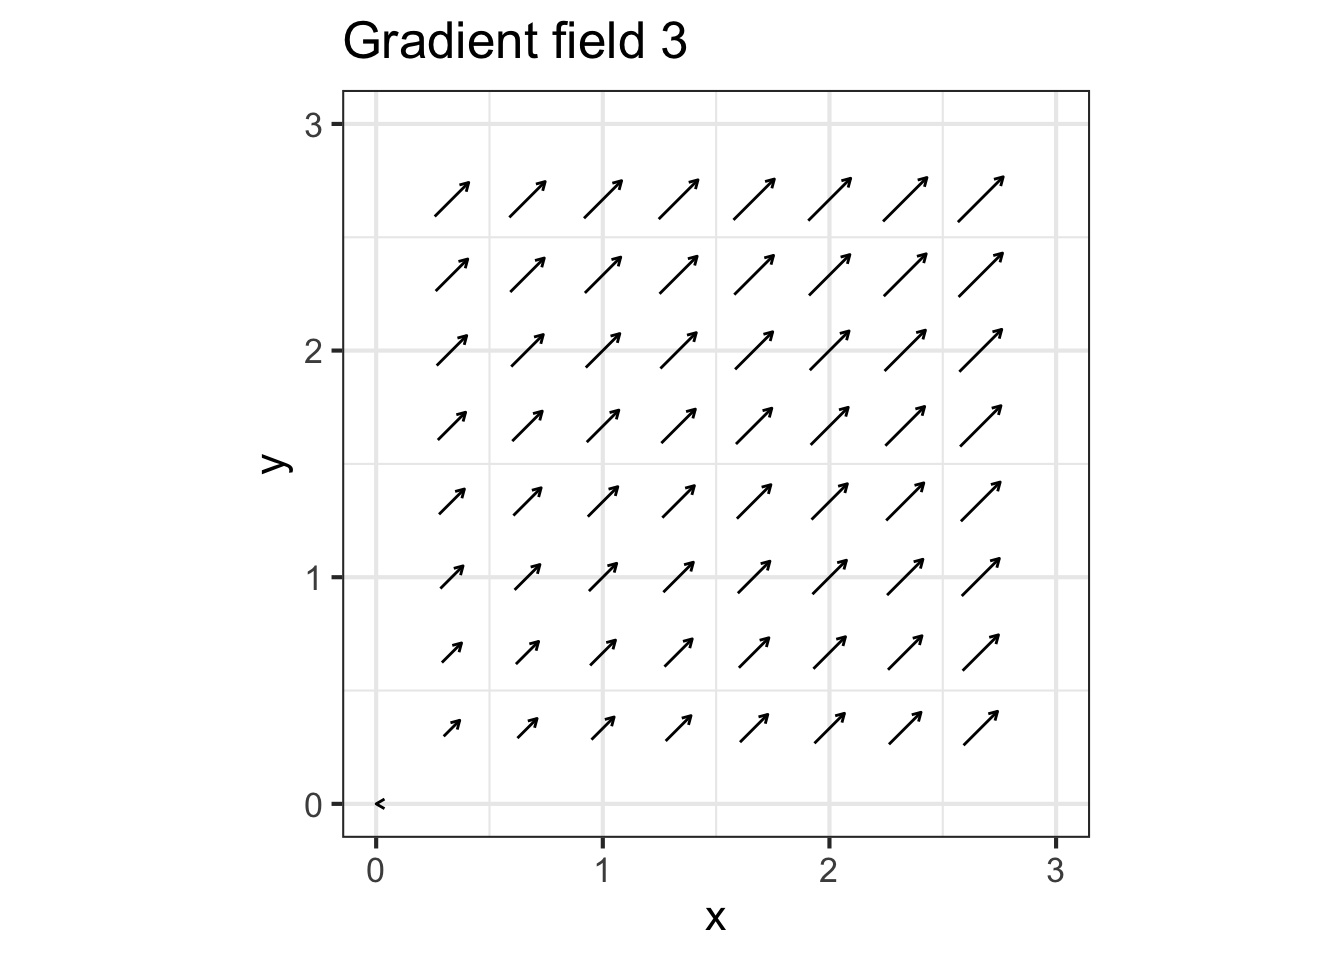
\includegraphics{Preliminaries/exercise-layout_files/figure-pdf/unnamed-chunk-42-1.pdf}

\textbf{Question C} For graph (C), which scale corresponds to the
pattern-book function?

\begin{enumerate}
\def\labelenumi{\roman{enumi}.}
\tightlist
\item
  {black{x}}\\
\item
  {blue{Correct.~The pattern-book sinusoid has a positive-going zero
  crossing at \(x=0\). That's the blue scale.}}\\
\item
  {neither{x}}\\
\item
  {both{xIt can't be both. There's only one pattern-book function.
  When you scale the input, it becomes a ``basic modeling function''.}}
\end{enumerate}

\hypertarget{exer.-8.3}{%
\section*{Exer. 8.3}\label{exer.-8.3}}
\addcontentsline{toc}{section}{Exer. 8.3}

\textbf{Exercise 8.3} ../Modeling/Exercises/scale-input-2.Rmd

Find the straight-line function that will give the value on the black
scale for each point \(x\) on the blue scale. The function will take the
blue-scale reading as input and produce the black-scale reading as
output, that is: \[\text{black}(x) \equiv a (x - x_0)\]

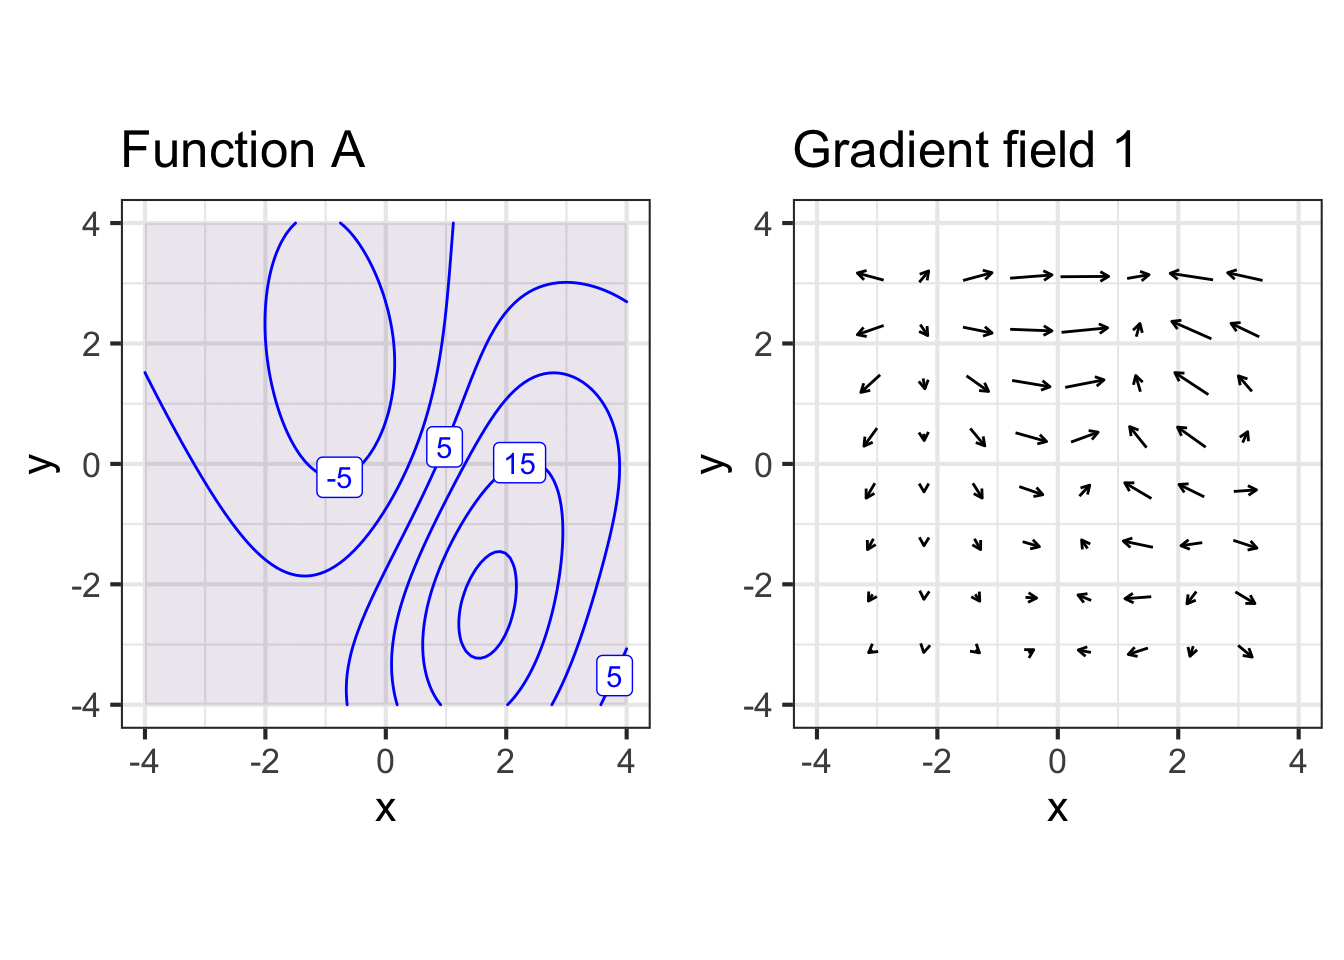
\includegraphics{Preliminaries/exercise-layout_files/figure-pdf/unnamed-chunk-46-1.pdf}

\textbf{Question A} For Graph A, which function maps blue \(x\) to the
value on the black scale?

\begin{enumerate}
\def\labelenumi{\roman{enumi}.}
\tightlist
\item
  {\$\text\{black\}(\text\{blue\}) \equiv \frac{1}{3} x\${Nice!~}}\\
\item
  {\$\text\{black\}(\text\{blue\}) \equiv 3, x\${xYou're going the wrong
  way, from black to blue.}}\\
\item
  {\$\text\{black\}(\text\{blue\}) \equiv x + 3\${xIs there a
  horiztontal shift?}}\\
\item
  {\$\text\{black\}(\text\{blue\}) \equiv x - 3\${xIs there a horizontal
  shift?}}
\end{enumerate}

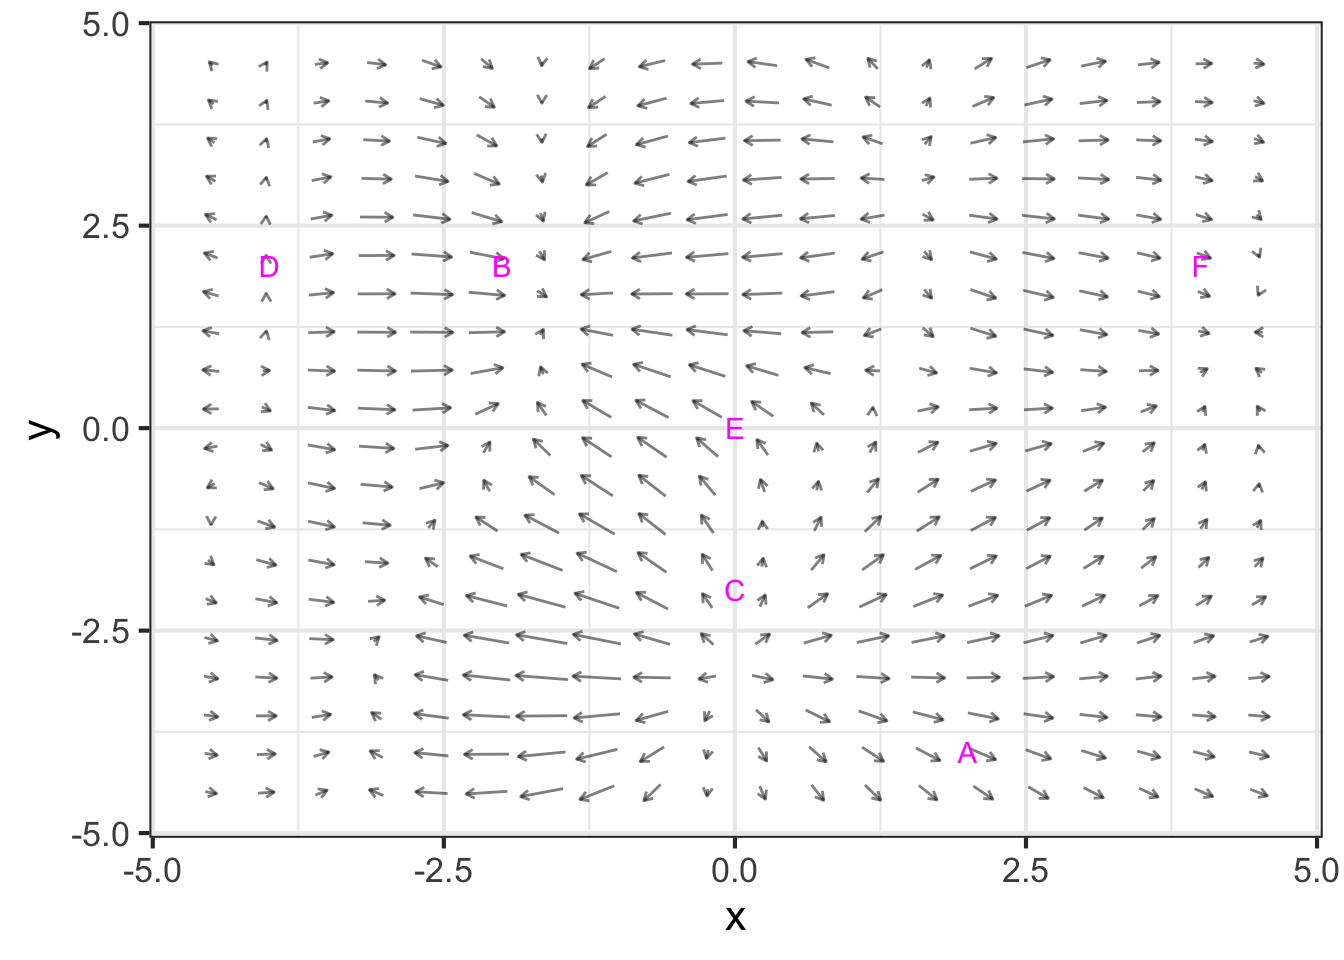
\includegraphics{Preliminaries/exercise-layout_files/figure-pdf/unnamed-chunk-48-1.pdf}

\textbf{Question B} For Graph B, which function maps blue \(x\) to the
value on the black scale?

\begin{enumerate}
\def\labelenumi{\roman{enumi}.}
\tightlist
\item
  {\$\text\{black\}(\text\{blue\}) \equiv -\frac{2}{3},x\${Nice!~}}\\
\item
  {\$\text\{black\}(\text\{blue\}) \equiv \frac{3}{2} x\${xLook
  carefully at the \(\pm\) signs on the scales.}}\\
\item
  {\$\text\{black\}(\text\{blue\}) \equiv \frac{2}{3} x\${xLook
  carefully at the \(\pm\) signs on the scales.}}\\
\item
  {\$\text\{black\}(\text\{blue\}) \equiv -\frac{3}{2}x\${xYou're going
  the wrong way, from black to blue.}}
\end{enumerate}

\includegraphics{Preliminaries/exercise-layout_files/figure-pdf/unnamed-chunk-50-1.pdf}

\textbf{Question C} For Graph C, which function maps blue \(x\) to the
value on the black scale?

\begin{enumerate}
\def\labelenumi{\roman{enumi}.}
\tightlist
\item
  {\$\text\{black\}(\text\{blue\}) \equiv \frac{1}{2}(x -
  2)\${Excellent!~Good. An interval of length 4 on the blue scale (say,
  from 2 to 6) becomes an interval of length 2 on the black scale. So
  you know that blue to black involves dividing by 2.}}\\
\item
  {\$\text\{black\}(\text\{blue\}) \equiv 3, x\${xIs there a shift}}\\
\item
  {\$\text\{black\}(\text\{blue\}) \equiv 2,x\${xIs there a shift?}}\\
\item
  {\$\text\{black\}(\text\{blue\}) \equiv 2,(x + 2)\${xYou're going the
  wrong way, from black to blue.}}
\end{enumerate}

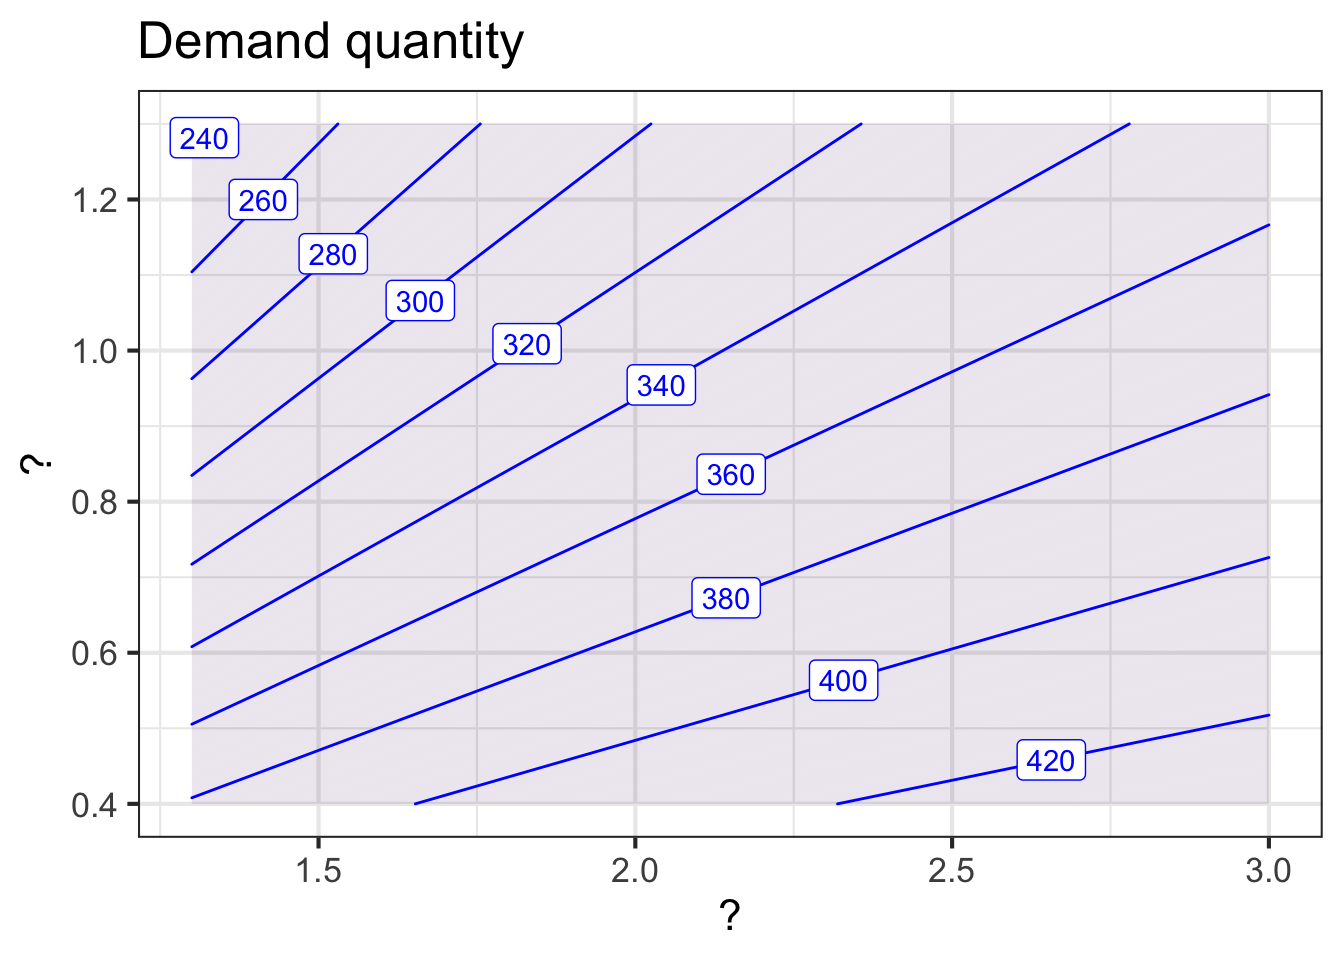
\includegraphics{Preliminaries/exercise-layout_files/figure-pdf/unnamed-chunk-52-1.pdf}

\textbf{Question D} For Graph D, which function maps blue \(x\) to the
value on the black scale?

\begin{enumerate}
\def\labelenumi{\roman{enumi}.}
\tightlist
\item
  {\$\text\{black\}(\text\{blue\}) \equiv \frac{2}{3} (x +
  3)\${Excellent!~}}\\
\item
  {\$\text\{black\}(\text\{blue\}) \equiv \frac{3}{2} (x - 3)\${x}}\\
\item
  {\$\text\{black\}(\text\{blue\}) \equiv \frac{3}{2} (x+1)\${x}}\\
\item
  {\$\text\{black\}(\text\{blue\}) \equiv rac\{3\}\{2\}(x - 2)\${xYou're
  going the wrong way, from black to blue.}}
\end{enumerate}

\hypertarget{exer.-8.1}{%
\section*{Exer. 8.1}\label{exer.-8.1}}
\addcontentsline{toc}{section}{Exer. 8.1}

\textbf{Exercise 8.1} ../Modeling/Exercises/fiducial-point.Rmd

Recall that each \textbf{\emph{basic modeling function}} is constructed
from the corresponding pattern-book function by scaling the input.

\[\text{pattern-book function}\ \ \underset{x\rightarrow a(x-x_0)}{\overset{\text{input scaling}}{\Large\Longrightarrow}} \ \ \text{basic modeling function}\]

Figure @ref(fig:fid-points) shows the pattern-book functions with some
added annotations. When the function has horizontal or vertical
asymptotes, the location is shown by orange arrows. There is also a blue
dot placed on the graph of functions with asymptotes. For functions
without asymptotes, there are two blue dots. The location of the
asymptotes and blue dots mark characteristic features of each function.
The positions of the blue dot and asymptotes, or the positions of the
two blue dots, are useful for figuring out the values of parameters in
basic modeling functions.

For example, the basic modeling reciprocal function is
\(g(x) \equiv \frac{1}{m (x-x_0)} + C\). The parameter \(C\) will be the
value where the horizontal asymptote crosses the vertical axis. The
parameter \(x_0\) will be the value where the vertical asymptote crosses
the horizontal axis. As for the parameter \(m\): find the input where
the function value is \(C+1\). Let's call that \(x^\star\). The
\(m = 1/(x^\star - x_0)\).

For the sinusoid, the blue dots mark the positive-going zero crossings
of the baseline. The horizontal distance between the blue dots is the
period parameter, \(P\). The horizontal position of either of the two
dots tells the phase offset \(x_0\).

\begin{figure}

{\centering 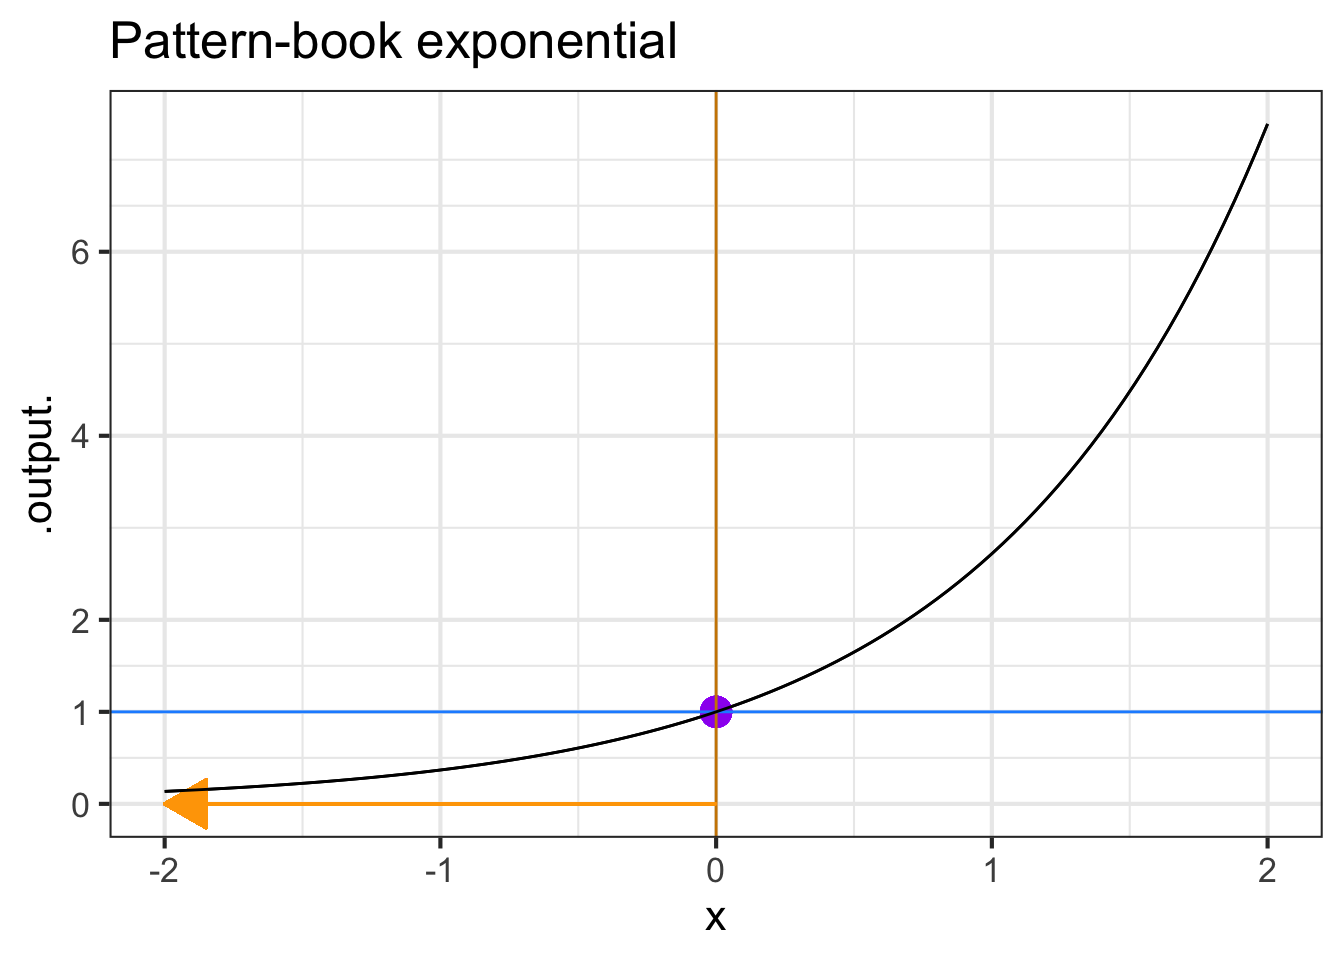
\includegraphics[width=0.5\textwidth,height=\textheight]{Preliminaries/exercise-layout_files/figure-pdf/fig-fid-points-1.pdf}

}

\caption{\label{fig-fid-points-1}\textbf{?(caption)}}

\end{figure}

\begin{figure}

{\centering 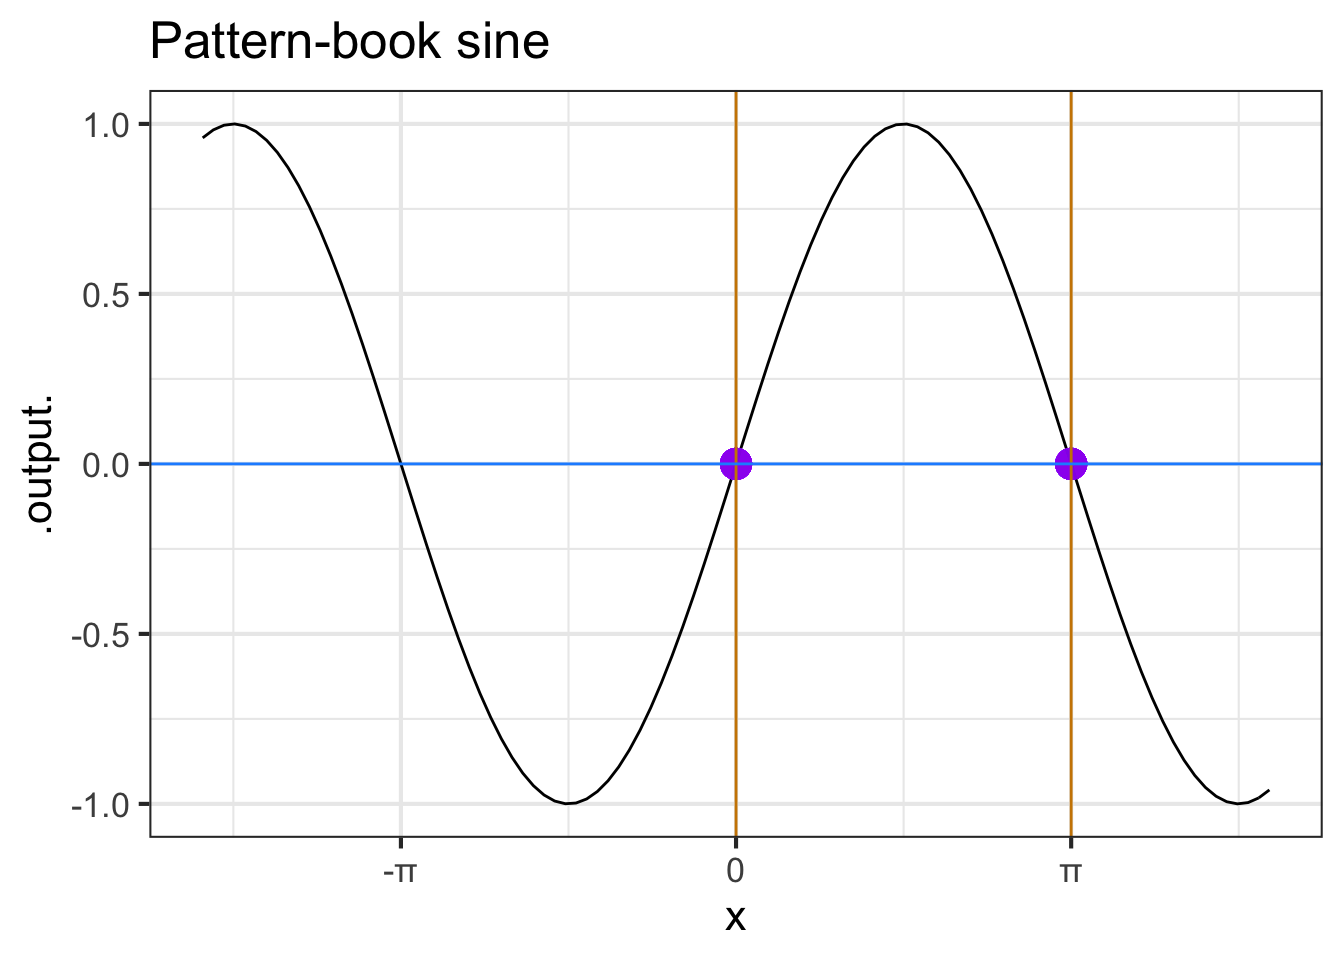
\includegraphics[width=0.5\textwidth,height=\textheight]{Preliminaries/exercise-layout_files/figure-pdf/fig-fid-points-2.pdf}

}

\caption{\label{fig-fid-points-2}\textbf{?(caption)}}

\end{figure}

\begin{figure}

{\centering 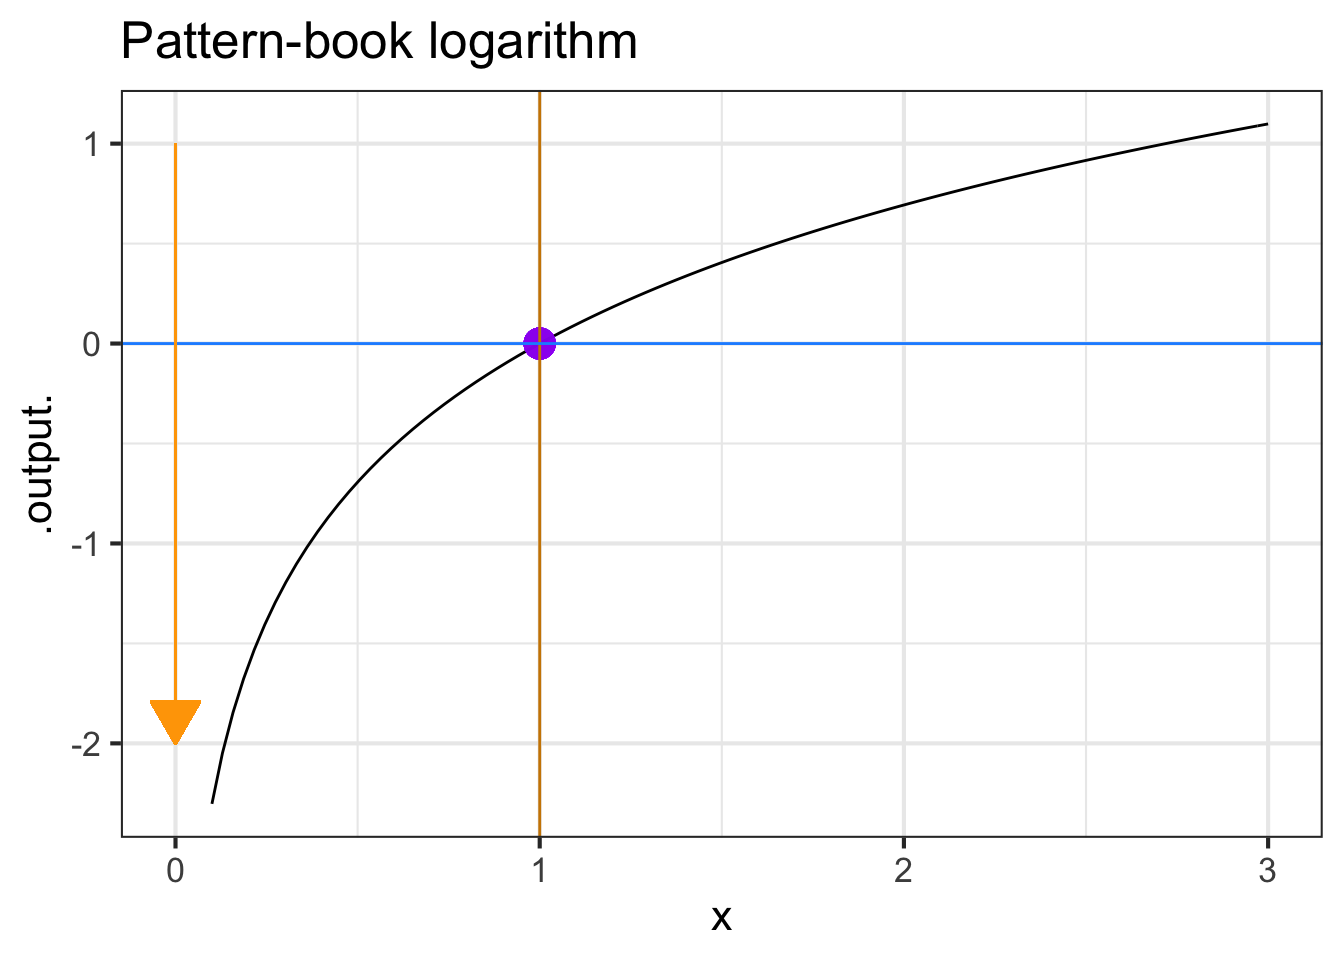
\includegraphics[width=0.5\textwidth,height=\textheight]{Preliminaries/exercise-layout_files/figure-pdf/fig-fid-points-3.pdf}

}

\caption{\label{fig-fid-points-3}\textbf{?(caption)}}

\end{figure}

\begin{figure}

{\centering 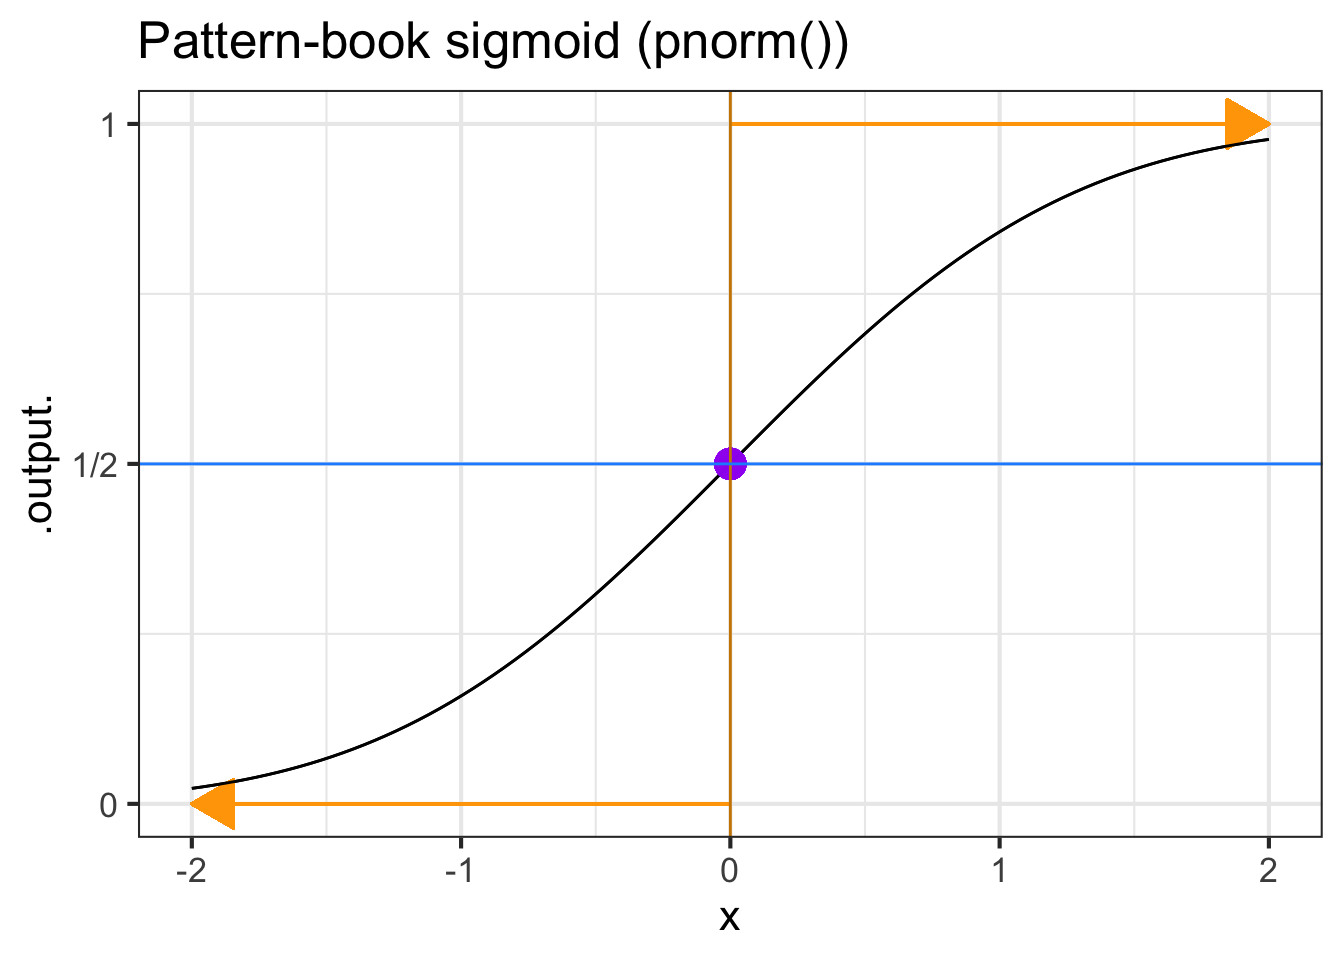
\includegraphics[width=0.5\textwidth,height=\textheight]{Preliminaries/exercise-layout_files/figure-pdf/fig-fid-points-4.pdf}

}

\caption{\label{fig-fid-points-4}\textbf{?(caption)}}

\end{figure}

\begin{figure}

{\centering 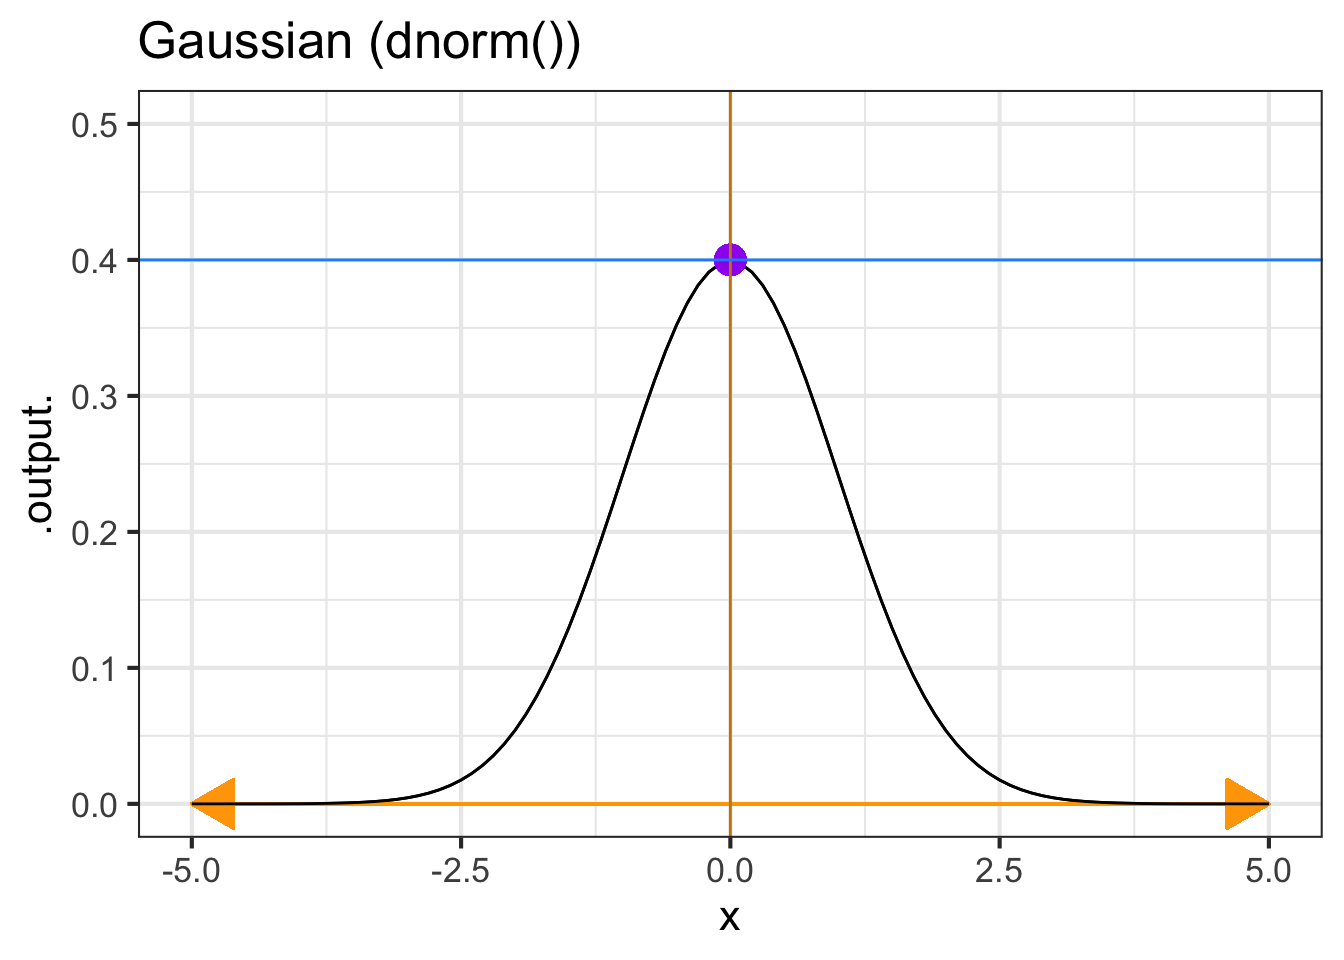
\includegraphics[width=0.5\textwidth,height=\textheight]{Preliminaries/exercise-layout_files/figure-pdf/fig-fid-points-5.pdf}

}

\caption{\label{fig-fid-points-5}\textbf{?(caption)}}

\end{figure}

\begin{figure}

{\centering 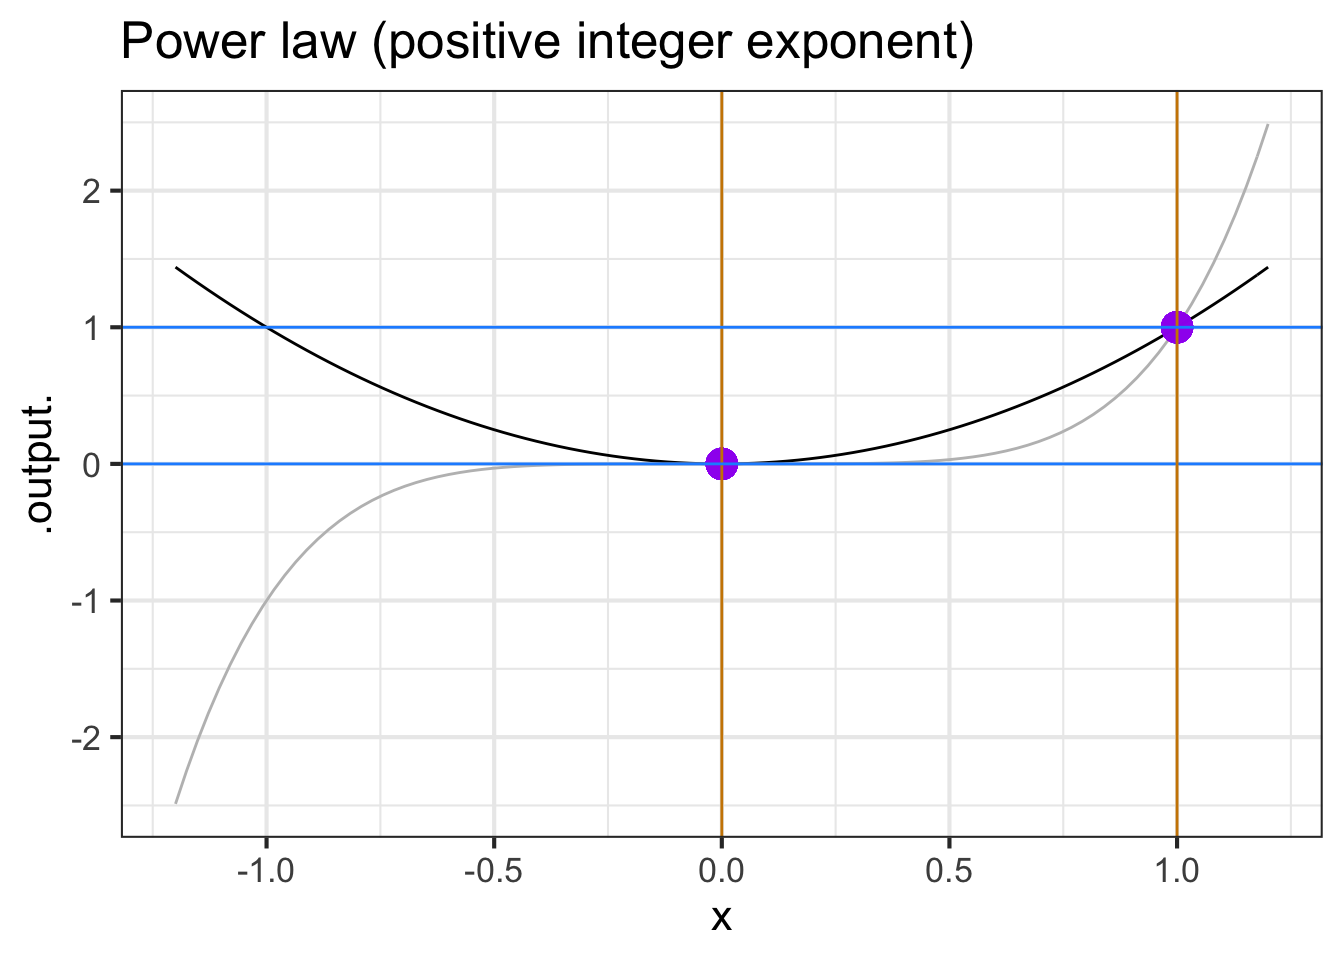
\includegraphics[width=0.5\textwidth,height=\textheight]{Preliminaries/exercise-layout_files/figure-pdf/fig-fid-points-6.pdf}

}

\caption{\label{fig-fid-points-6}\textbf{?(caption)}}

\end{figure}

\begin{figure}

{\centering 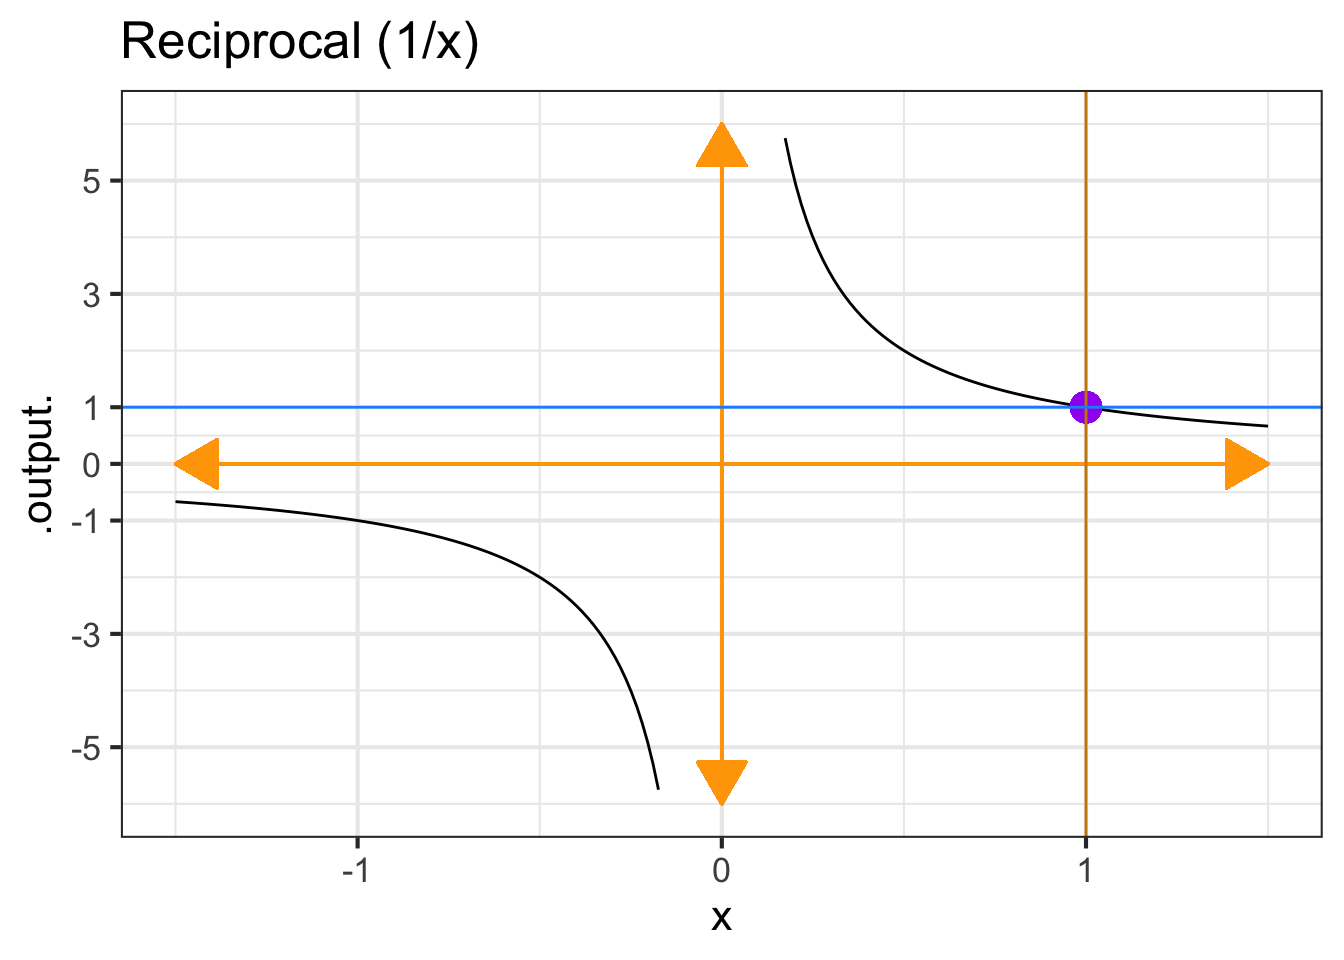
\includegraphics[width=0.5\textwidth,height=\textheight]{Preliminaries/exercise-layout_files/figure-pdf/fig-fid-points-7.pdf}

}

\caption{\label{fig-fid-points-7}\textbf{?(caption)}}

\end{figure}

Each of the following plots shows a basic modeling function whose input
scaling has the form \(x - x_0\). Your job is to figure out from the
graph what is the numerical value of \(x_0\). (Hint: For simplicity,
\(x_0\) in the questions will always be an integer.)

\includegraphics{Preliminaries/exercise-layout_files/figure-pdf/unnamed-chunk-55-1.pdf}

\textbf{Question A} In plot (A), what is \(x_0\)?

~~~~{-2{x}}~~~~~~~{-1{x}}~~~~~~~{0{x}}~~~~~~~{1{︎X
}}~~~~~~~{2{\(\heartsuit\ \)Right. Look for the input that generates the
peak output value.}}

\includegraphics{Preliminaries/exercise-layout_files/figure-pdf/unnamed-chunk-57-1.pdf}

\textbf{Question B} In plot (B), what is \(x_0\)?

~~~~{-2{x}}~~~~~~~{-1{\(\heartsuit\ \)The fiducial point is a
positive-going zero crossing.}}~~~~~~~{0{x}}~~~~~~~{1{︎X
}}~~~~~~~{2{x}}

\includegraphics{Preliminaries/exercise-layout_files/figure-pdf/unnamed-chunk-59-1.pdf}

\textbf{Question C} In plot (C), what is \(x_0\)?

~~~~{-2{x}}~~~~~~~{-1{x}}~~~~~~~{0{︎X
}}~~~~~~~{1{\(\heartsuit\ \)The vertical asymptote is the
clue.}}~~~~~~~{2{x}}

\includegraphics{Preliminaries/exercise-layout_files/figure-pdf/unnamed-chunk-61-1.pdf}

\textbf{Question D} In plot (D), what is \(x_0\)?

\begin{enumerate}
\def\labelenumi{\roman{enumi}.}
\tightlist
\item
  {-2{x}}\\
\item
  {-1{x}}\\
\item
  {0{x}}\\
\item
  {1{Excellent!~The input where the output is half way between the two
  horizontal asymptotes}}\\
\item
  {2{x}}
\end{enumerate}

\includegraphics{Preliminaries/exercise-layout_files/figure-pdf/unnamed-chunk-63-1.pdf}

\textbf{Question E} In plot (E), what is \(x_0\)?

~~~~{-2{\(\heartsuit\ \)Right. The location of the vertical asymtote is
the clue.}}~~~~~~~{-1{x}}~~~~~~~{0{x}}~~~~~~~{1{x}}~~~~~~~{2{x}}

\hypertarget{exer.-8.5}{%
\section*{Exer. 8.5}\label{exer.-8.5}}
\addcontentsline{toc}{section}{Exer. 8.5}

\textbf{Exercise 8.5} ../Modeling/Exercises/two-sines.Rmd

The graph shows a linear combination of two sinusoids, one of period 0.6
and the other of period 2. There is also a baseline shift. That is, the
graph shows the function:

\[A_1 \sin\left(\frac{2\pi}{2}t\right) + A_2 \sin\left(\frac{2\pi}{0.6} (t-.3)\right) + A_3\]

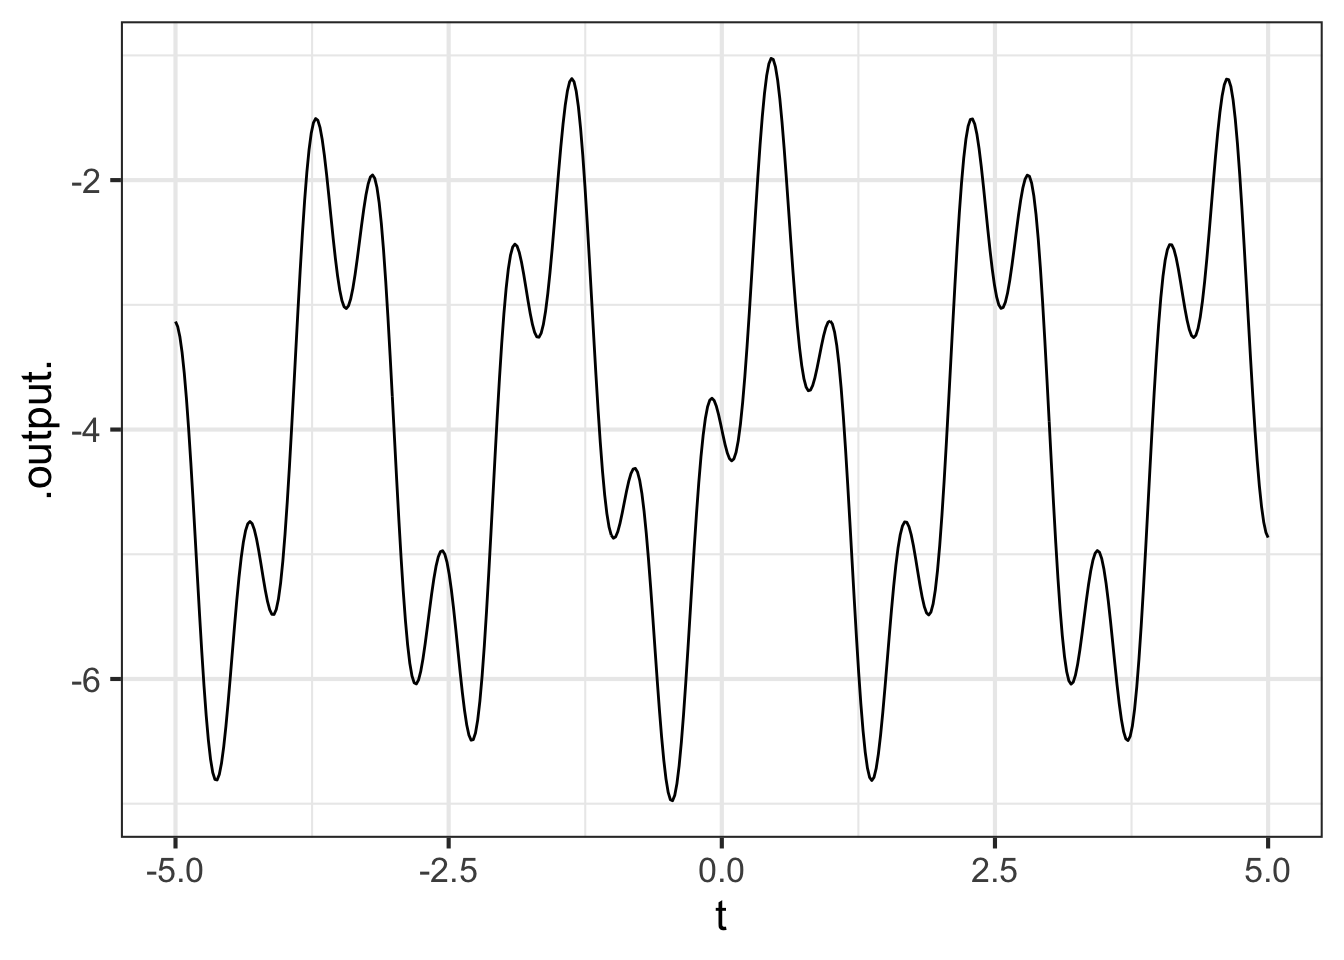
\includegraphics{Preliminaries/exercise-layout_files/figure-pdf/two-sines-1-1.pdf}

\textbf{Question A} What is \(A_3\)?

~~~~{-4{\(\heartsuit\ \)}}~~~~~~~{-2{x}}~~~~~~~{0{x}}~~~~~~~{2{︎X
}}~~~~~~~{4{x}}

\textbf{Question B} What is \(A_1\)?

~~~~{0{x}}~~~~~~~{1{x}}~~~~~~~{2{\(\heartsuit\ \)}}~~~~~~~{3.5{x}}

\textbf{Question C} What is \(A_2\)?

~~~~{0{x}}~~~~~~~{1{\(\heartsuit\ \)}}~~~~~~~{2{x}}~~~~~~~{3.5{x}}

\hypertarget{exer.-8.7}{%
\section*{Exer. 8.7}\label{exer.-8.7}}
\addcontentsline{toc}{section}{Exer. 8.7}

\textbf{Exercise 8.7} ../Modeling/Exercises/walnut-run-dish.Rmd

Turn this into a guided problem to find the input and output scaling
that turns \(\sin()\) into the day-length versus day-of-year.

To illustrate, suppose that \(f(x)\) is one of the pattern-book
function, say, \(\sin()\). The input to pattern-book \(\sin()\) must
always be a pure number and the output will always be a pure number.
Consider a phenomenon that shows oscillatory behavior, for instance the
length of daylight (in hours) as a function of the day-of-the-year (1 to
365, in days). The output of the modeling function is a quantity in
hours, the input is a quantity in days. Neither this input nor the
output are pure numbers.

To use the pattern \(\sin()\) as a basis for modeling, we replace the
input name \(x\) with a straight-line function: \(x(t) = a t + b\). This
gives us the function \[\sin(a t + b)\] where \(a\) and \(b\) are
parameters. If \(t\) is to be the day-of-year in units of days, then the
parameter \(a\) will have units ``per day,'' so that \(a t\) will be a
pure number.

The output of the function \(\sin(a t + b)\) will be a pure number. In
order to translate this into a quantity such as length of daylight, we
apply another straight-line function, for instance
\[\text{daylight}(y) \equiv A y + B\] where \(y\) stands for the output
from \(\sin(a t + b)\) for any input \(t\). Putting this all together,
we have the function \[\text{daylight}(t) = A \sin(a t + b) + B\ ,\] a
function with four parameters: \(a\), \(b\), \(A\), and \(B\).

For example, for a location at latitude 40\(^\circ\)N, the length of
daylight is approximately
\[\text{daylight}_{40^\circ}(t) = 2.75 \sin(0.0173 t - 0.155) + 12\ ,\]
where \(t\) is in days (January 1 is \(t=1\) and December 31 is
\(t=365\)), 2.75 and 12 are in hours, 0.0173 is ``per day'' and 0.155 is
a pure number.

Keep in mind that the straight-line function is often written
\(\line(t) = a\left(t-t_0\right)\). In this form, the daylight()
function would be written
\[\text{daylight}_{40^\circ}(t) = 2.75 \sin(0.0173 \left(t - 9\right) + 12\ ,\]
where the 9 is in days.

\hypertarget{exer.-8.9}{%
\section*{Exer. 8.9}\label{exer.-8.9}}
\addcontentsline{toc}{section}{Exer. 8.9}

\textbf{Exercise 8.9} ../Modeling/Exercises/boy-put-sofa.Rmd

Convert this to a guided exercise on finding the appropriate scale
conversion parameters.

Figure @ref(fig:covid-scale) shows the model we fit to the COVID-19 data
for the cumulative number of confirmed cases for each day in March:
\(\text{cases(day)} = e^{0.19(\text{day}- -32)}\)

\begin{figure}

{\centering \includegraphics{Preliminaries/exercise-layout_files/figure-pdf/fig-covid-scale-1.pdf}

}

\caption{\label{fig-covid-scale}A graph of the pattern-book exponential
with an additional scale displayed (blue) to match it to the COVID-19
data}

\end{figure}

The function being drawn is simply \(e^x\): a function from the pattern
book. The black horizontal scale shows \(x\), the input to the
pattern-book function. Where does that value of \(x\) come from? It's
\(0.19(\text{day} - -32)\), where day is the number of the day in March.
For instance, on March 20, day\(=10\) and
\(0.19*(\text{day}- -32) = 9.88\). You can see that 20 on the blue scale
matches 10 on the black scale. The model says that on day 20 (blue
scale) the input to the pattern-book function will be 9.88 (black
scale). Plugging the input 9.88 into the pattern-book exponential gives
\(e^{9.88} = 19536 \approx 20,000\) cases.

The pattern-book function does not give a good model of the COVID case
numbers. But if we scale the input before applying the pattern-book
function, we are effectively laying a new axis, the blue one in Figure
@ref(fig:covid-scale), that is stretched and shifted from the
pattern-book input (blackscale). Using the blue axis lets us read off
the number of cases as a function of the day in March.

Input scaling empowers the pattern-book functions to model a huge
variety of phenomena. There's just one exponential function and it
always looks the same. But there is a huge variety of ways to draw a
blue axis, that is, to scale the input. With input scaling, the
pattern-book function is tailored to become one of our basic modeling
functions.
\[\underbrace{e^x}_\text{pattern-book function}\  \text{versus}\  \underbrace{e^{k(x-x_0)}}_\text{basic modeling function}\]

\hypertarget{exer.-9.1}{%
\section*{Exer. 9.1}\label{exer.-9.1}}
\addcontentsline{toc}{section}{Exer. 9.1}

\textbf{Exercise 9.1} ../Modeling/Exercises/seahorse-build-pot.Rmd

Turn this into a programming activity, where they need to introduce the
function \texttt{deg2rad()}.

\begin{rmosaic}
Composing functions is very common in computer programming. Consider
these two functions

\end{rmosaic}

A computer implementation must look different, since \(L\) and
\(\delta\) are typically provided in degrees while the \texttt{tan()}
and other trigonometric functions in most computer languages expect
units of radians. The conversion is easy:
\(\text{deg2rad}(d) \equiv \frac{\pi}{180} d\). The conversion the other
way is \(\text{rad2deg}(r) \equiv \frac{180}{\pi} r\).

In order to get the day-length formula to work in a computer, we can
compose the \(\tan()\) function with \texttt{deg2rad()}. The output of
\texttt{acos()} is in radians, so we have to convert it back to degrees.
Like this:

\begin{Shaded}
\begin{Highlighting}[]
\NormalTok{day\_length }\OtherTok{\textless{}{-}} \FunctionTok{makeFun}\NormalTok{(}
\NormalTok{  (}\DecValTok{2}\SpecialCharTok{/}\DecValTok{15}\NormalTok{)}\SpecialCharTok{*}\FunctionTok{rad2deg}\NormalTok{(}
    \FunctionTok{acos}\NormalTok{(}
      \SpecialCharTok{{-}}\FunctionTok{tan}\NormalTok{(}\FunctionTok{deg2rad}\NormalTok{(L))}\SpecialCharTok{*}\FunctionTok{tan}\NormalTok{(}\FunctionTok{deg2rad}\NormalTok{(d))}
\NormalTok{    )}
\NormalTok{  ) }\SpecialCharTok{\textasciitilde{}}\NormalTok{ L }\SpecialCharTok{\&}\NormalTok{ d)}
\end{Highlighting}
\end{Shaded}

Now to make a plot of day length as a function of day of the year. Of
course, \texttt{day\_length(L,\ d)} does not take day of the year into
account. What's missing is to know the declination of the sun as a
function of calendar day.

The input is a number \(n\) that runs from 0 at the start of January 1st
to 365 at the end of December 31. In terms of this input, the
declination of the sun is known to be approximately ::: \{.cell\}

\begin{Shaded}
\begin{Highlighting}[]
\NormalTok{delta\_sun }\OtherTok{\textless{}{-}} \FunctionTok{makeFun}\NormalTok{(}\SpecialCharTok{{-}}\FloatTok{23.44}\SpecialCharTok{*}\FunctionTok{cos}\NormalTok{((}\DecValTok{2}\SpecialCharTok{*}\NormalTok{pi}\SpecialCharTok{/}\DecValTok{365}\NormalTok{)}\SpecialCharTok{*}\NormalTok{(n}\SpecialCharTok{+}\DecValTok{10}\NormalTok{) ) }\SpecialCharTok{\textasciitilde{}}\NormalTok{ n)}
\end{Highlighting}
\end{Shaded}

:::

Composing \texttt{day\_length()} with \texttt{delta\_sun()} (on the
\texttt{d} argument only), and setting the latitude to be, say,
\(39^\circ\)N, we get a function of day of year \texttt{n}: :::
\{.cell\}

\begin{Shaded}
\begin{Highlighting}[]
\FunctionTok{slice\_plot}\NormalTok{(}
  \FunctionTok{day\_length}\NormalTok{(}\DecValTok{39}\NormalTok{, }\FunctionTok{delta\_sun}\NormalTok{(n)) }\SpecialCharTok{\textasciitilde{}}\NormalTok{ n, }
  \FunctionTok{domain}\NormalTok{(}\AttributeTok{n=}\FunctionTok{c}\NormalTok{(}\DecValTok{0}\NormalTok{,}\DecValTok{365}\NormalTok{))}
\NormalTok{  )}
\end{Highlighting}
\end{Shaded}

\begin{figure}[H]

{\centering \includegraphics{Preliminaries/exercise-layout_files/figure-pdf/unnamed-chunk-70-1.pdf}

}

\end{figure}

:::

\hypertarget{exer.-9.2}{%
\section*{Exer. 9.2}\label{exer.-9.2}}
\addcontentsline{toc}{section}{Exer. 9.2}

\textbf{Exercise 9.2} ../Modeling/Exercises/dog-dive-kitchen.Rmd

Make this about identifying the functions being composed, multiplied, or
linearly combined.

\textbf{All together now!}

Two or all three of the techniques for combining functions---linear
combinations, function composition, and function multiplication---can be
used in the same function.

Consider the function for the length of the day
\[\text{daylight}(L, \delta) \equiv \frac{2}{15} \arccos\left(-\tan(L)*\tan(\delta)\right)\]
The 2/15 is scaling the output of \(\arccos()\). The \(\arccos()\) is
being composed with an interior function that is itself a scaled product
of two functions.

\hypertarget{exer.-9.3}{%
\section*{Exer. 9.3}\label{exer.-9.3}}
\addcontentsline{toc}{section}{Exer. 9.3}

\textbf{Exercise 9.3} ../Modeling/Exercises/pine-bring-dish.Rmd

Make this a computer exercise about multiplying functions. Try to play
the sounds they create.

This example concerns a bit of familiar technology: music synthesis.
Generating a pure tone electronically is easily done using a sinusoid.
Generating a note with rich instrumental timbre can be accomplished by a
linear combination of sinusoids. Of course, the note will be localized
in time. This could be accomplished by multiplying the sinusoids by a
gaussian function envelope.

It turns out that the gaussian function, \texttt{dnorm()}, does not
generate a realistic sound. Instead, a more complicated envelope is
used, such as the
\href{https://en.wikipedia.org/wiki/Envelope_(music)}{ADSR function}
shown in Figure @ref(fig:ADSR). The function has six (!) parameters: the
time the key is pressed, the duration A of the ``attack'' phase when the
sound amplitude is increasing in response to the impulse imposed on the
key, a decay of duration D to an output level S that lasts until the key
is released, then a decay to zero over duration R. It's reasonable to
think of the D and S phases as a piecewise linear approximation to
exponential decay.

\begin{figure}

{\centering 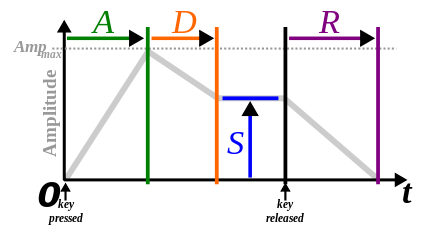
\includegraphics[width=0.65\textwidth,height=\textheight]{Preliminaries/www/adsr.png}

}

\caption{\label{fig-ADSR}The ADSR envelope function used in music
synthesis consists of 6 pieces including zero output before the key is
pressed and after the pulse ends.
\href{https://en.wikipedia.org/wiki/Envelope_(music)}{Source}}

\end{figure}

\hypertarget{exer.-9.4}{%
\section*{Exer. 9.4}\label{exer.-9.4}}
\addcontentsline{toc}{section}{Exer. 9.4}

\textbf{Exercise 9.4} ../Modeling/Exercises/bigger-two.Rmd

The function \texttt{bigger()} is defined piecewise in terms of two
extremely simple functions. Each of the two simple functions has a
contour plot with contours that are parallel. The piecewise combination
of the simple functions has a more complicated contour plot, with each
simple function's parallel contours showing up in half of the domain.
We'll call these ``pieces'' of the domain.

\begin{Shaded}
\begin{Highlighting}[]
\NormalTok{bigger }\OtherTok{\textless{}{-}} \FunctionTok{makeFun}\NormalTok{(}\FunctionTok{ifelse}\NormalTok{(y }\SpecialCharTok{\textgreater{}}\NormalTok{ x, y, x) }\SpecialCharTok{\textasciitilde{}}\NormalTok{ x }\SpecialCharTok{+}\NormalTok{ y)}
\FunctionTok{contour\_plot}\NormalTok{(}\FunctionTok{bigger}\NormalTok{(x,y) }\SpecialCharTok{\textasciitilde{}}\NormalTok{ x}\SpecialCharTok{+}\NormalTok{y, }\FunctionTok{domain}\NormalTok{(}\AttributeTok{x=}\FunctionTok{c}\NormalTok{(}\SpecialCharTok{{-}}\DecValTok{2}\NormalTok{,}\DecValTok{2}\NormalTok{), }\AttributeTok{y=}\FunctionTok{c}\NormalTok{(}\SpecialCharTok{{-}}\DecValTok{2}\NormalTok{,}\DecValTok{2}\NormalTok{)))}
\end{Highlighting}
\end{Shaded}

\begin{figure}[H]

{\centering \includegraphics{Preliminaries/exercise-layout_files/figure-pdf/unnamed-chunk-77-1.pdf}

}

\end{figure}

\textbf{Question A} Which of the following best describes the two pieces
of the domain?

\begin{enumerate}
\def\labelenumi{\roman{enumi}.}
\tightlist
\item
  {One is above and to the left of the line of identity (that is,
  \(y=x\)) and the other is below and to the right of that
  line.{Correct.~}}\\
\item
  {One is \(x > 0\) and the other \(x \leq 0\){x}}\\
\item
  {One is \(x > 0\) and the other \(y \leq 0\){x}}
\end{enumerate}

\hypertarget{exer.-9.5}{%
\section*{Exer. 9.5}\label{exer.-9.5}}
\addcontentsline{toc}{section}{Exer. 9.5}

\textbf{Exercise 9.5} ../Modeling/Exercises/beech-ride-table.Rmd

The Heaviside function has two asymptotes.

\begin{enumerate}
\def\labelenumi{\arabic{enumi}.}
\item
  Are they horizontal or vertical asymptotes?
\item
  What are their values?
\end{enumerate}

\hypertarget{exer.-9.6}{%
\section*{Exer. 9.6}\label{exer.-9.6}}
\addcontentsline{toc}{section}{Exer. 9.6}

\textbf{Exercise 9.6} ../Modeling/Exercises/shark-rise-kitchen.Rmd

TURN THIS INTO AN EXERCISE

Open an R console and see what happens when you make the plot.

\begin{Shaded}
\begin{Highlighting}[]
\FunctionTok{slice\_plot}\NormalTok{(}\FunctionTok{log}\NormalTok{(x) }\SpecialCharTok{\textasciitilde{}}\NormalTok{ x, }\FunctionTok{domain}\NormalTok{(}\AttributeTok{x=}\FunctionTok{c}\NormalTok{(}\SpecialCharTok{{-}}\DecValTok{5}\NormalTok{,}\DecValTok{5}\NormalTok{)))}
\end{Highlighting}
\end{Shaded}

\hypertarget{exer.-10.1}{%
\section*{Exer. 10.1}\label{exer.-10.1}}
\addcontentsline{toc}{section}{Exer. 10.1}

\textbf{Exercise 10.1} ../Modeling/Exercises/NOAA.Rmd

Many printed tables are meant to be used as functions; you plug in the
input values and read off the output. Here's a table published by the
National Oceanic and Atmospheric Administration for the
\href{https://en.wikipedia.org/wiki/Heat_index}{heat index}, a way of
summarizing the perceived comfort (or discomfort) of summer-like weather
conditions.

\begin{figure}

{\centering 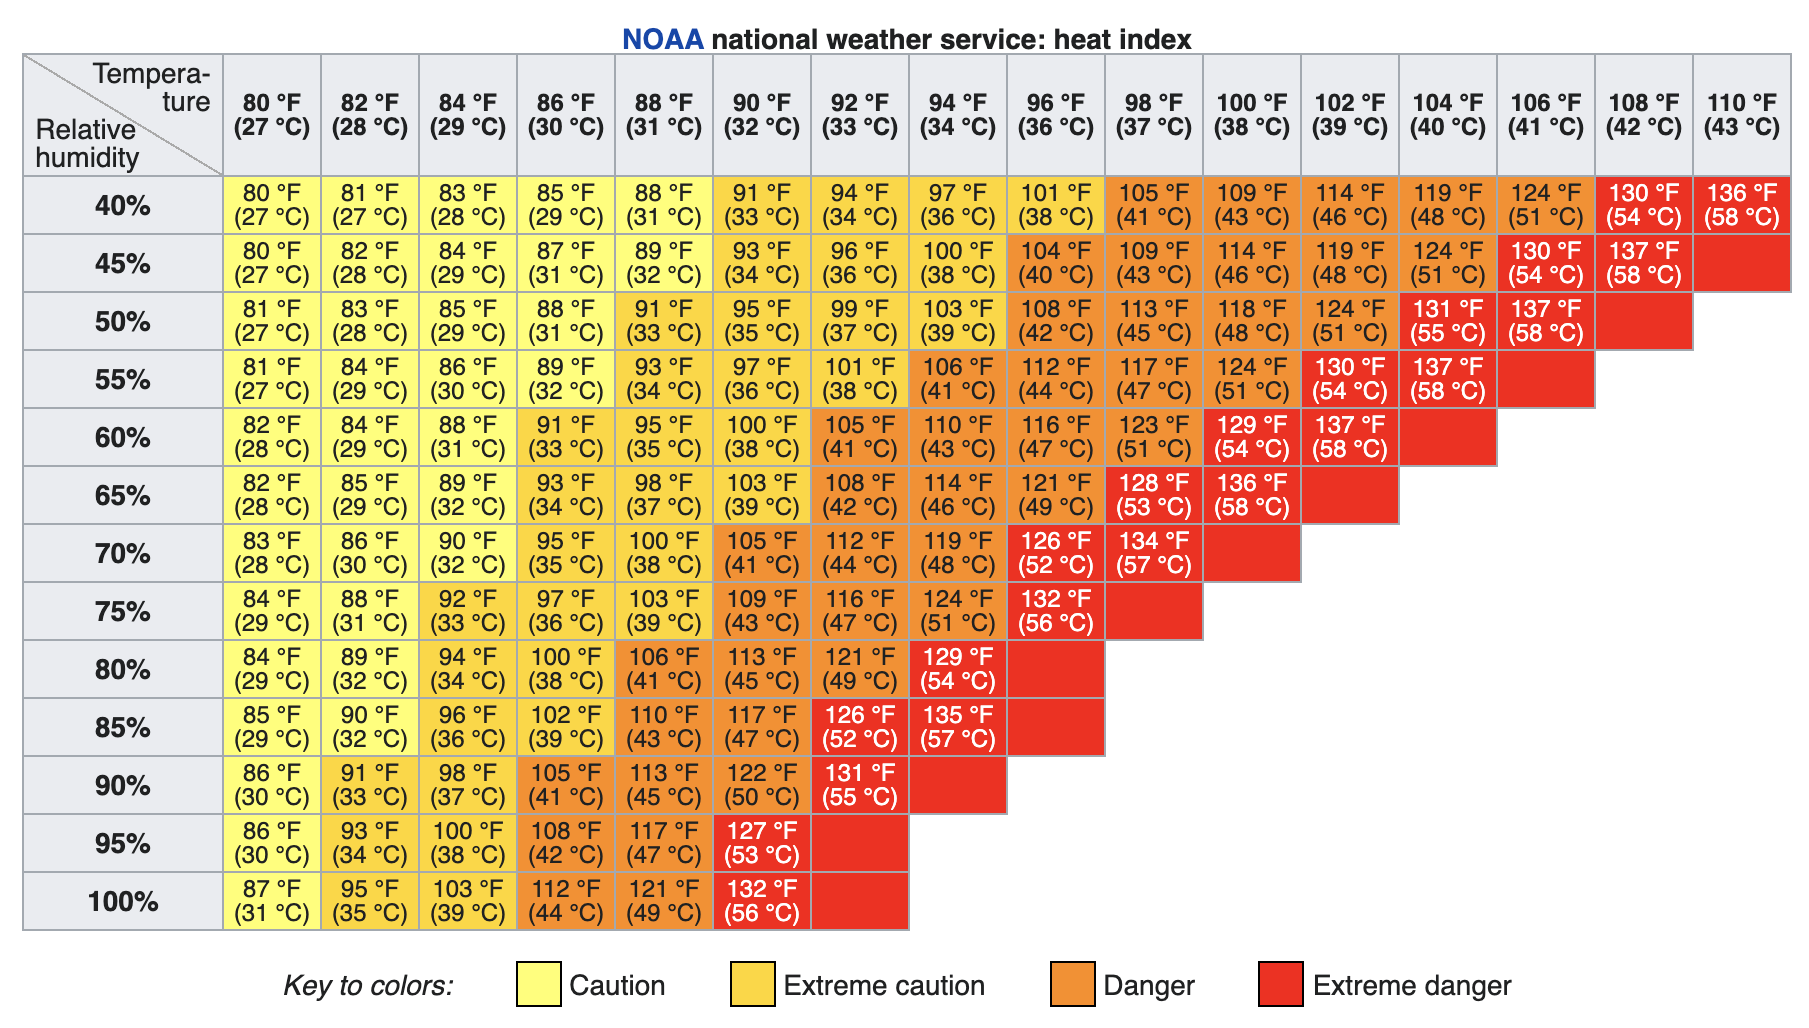
\includegraphics[width=0.9\textwidth,height=\textheight]{Preliminaries/www/heat-index.png}

}

\end{figure}

\textbf{Question A} What are the inputs to the heat-index function

\begin{enumerate}
\def\labelenumi{\roman{enumi}.}
\tightlist
\item
  {temperature and relative humidity{Nice!~}}\\
\item
  {temperature and wind speed{xThose are the inputs to the wind-chill
  function, not the heat index.}}\\
\item
  {temperature, latitude, and longitude{xThe heat index doesn't depend
  on location.}}
\end{enumerate}

The table shows three different functions:

\begin{enumerate}
\def\labelenumi{\arabic{enumi}.}
\tightlist
\item
  The heat index in \(^\circ\) F.
\item
  The heat index in \(^\circ\) C.
\item
  A caution warning level.
\end{enumerate}

\textbf{Question B} For inputs of 70\% relative humidity and
\(88^{\circ}\) F, what are the outputs of the three functions?

\begin{enumerate}
\def\labelenumi{\roman{enumi}.}
\tightlist
\item
  {\(100^{\circ}\) F, \(38^\circ\) C, and ``extreme
  caution''.{Good.~}}\\
\item
  {\(100^\circ\) F, \(38^\circ\) C, and ``danger''.{xCheck again!}}\\
\item
  {\(100^\circ\) F, \(33^\circ\) C, and ``extreme caution''.{x33C does
  is not the same temperature as 100F.}}
\end{enumerate}

\textbf{Question C} Holding the relative humidity at 70\%, how much
would the ambient temperature have to increase (from \(88^\circ\) F) to
change the caution-level output to ``dangerous''?

\begin{enumerate}
\def\labelenumi{\roman{enumi}.}
\tightlist
\item
  {Increase by \(2^\circ\) F{Good.~}}\\
\item
  {Increase by \(6^\circ\) F{xIt looks like you're increasing the
  humidity to the point where the heat index is \(106^circ\) F. But we
  asked you how much the temperature \emph{input} has to change, not the
  heat-index output.}}\\
\item
  {Increase relative humidity to 80\%.{xIt's true that at
  \(100^\circ\) F and 80\% humidity, the caution-index is ``dangerous''.
  But the problem specified holding humidity constant.}}
\end{enumerate}

\textbf{Question D} From a starting point of \(88^\circ\) F and 70\%
humidity, what is the slope of the increase in heat index when moving to
80\% humidity.

\begin{enumerate}
\def\labelenumi{\roman{enumi}.}
\tightlist
\item
  {\(6^\circ\) F per 10 percentage points humidity{Nice!~}}\\
\item
  {\(6^\circ\) F{xA slope is always ``rise over run''. You've got the
  rise right, but what about the run?}}\\
\item
  {\(6^\circ\) F per 80\% humidity.{xThe slope is the change in output
  divided by the change in input, i.e.~``rise over run''. 80\% is the
  humidity at the endpoint, but the run is the change in humidity from
  the starting point to the endpoint.}}
\end{enumerate}

\textbf{Question E} What is the heat-index output when the inputs are
52\% relative humidity and \(91^\circ\) F? Choose the best answer.

\begin{enumerate}
\def\labelenumi{\roman{enumi}.}
\tightlist
\item
  {\(98.4^\circ\) F{Good.~Of course, the 4 in the last digit is sketchy,
  but it's reasonable to calculate the interpolated output by averaging
  over neighboring outputs.}}\\
\item
  {\(101^\circ\) F{xThat's the output at 55\% humidity and
  \(92^\circ\) F.}}\\
\item
  {The table doesn't say.{xWhile it's true that there is no table
  entry specifically for 52\% and \(91^\circ\) F, you can make a very
  reasonable guess by \emph{interpolation}, that is, reading between the
  rows and columns.}}
\end{enumerate}

\textbf{Question F} True or false: The caution-level output could have
been presented as a function of just one input, rather than needing both
temperature and humidity.

\begin{enumerate}
\def\labelenumi{\roman{enumi}.}
\tightlist
\item
  {TRUE{Good.~The caution-level output is not a function of ambient
  temperature alone or of humidity alone. But if you know the
  heat-index, you know that caution level exactly.}}\\
\item
  {FALSE{xNotice that the caution-level output is the same for any
  given level of the heat index, regardless of the ambient temperature
  or humidity separately.}}
\end{enumerate}

The US National Weather Service also publishes a heat index graphic, the
one below.

\begin{verbatim}
Warning in normalizePath("www/weather-service-heatindex.png"): path[1]="www/
weather-service-heatindex.png": No such file or directory
\end{verbatim}

\begin{figure}

{\centering 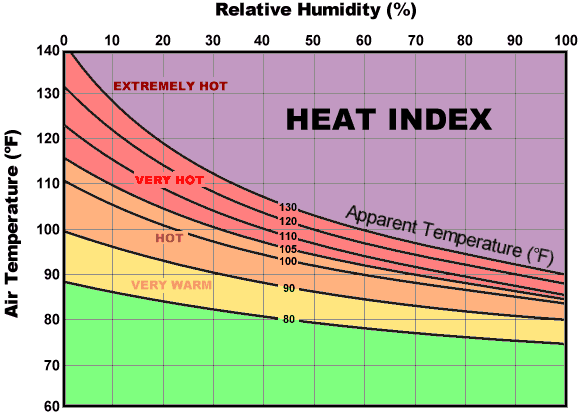
\includegraphics[width=0.9\textwidth,height=\textheight]{Preliminaries/www/weather-service-heatindex.png}

}

\end{figure}

\href{https://www.weather.gov/images/oun/wxsafety/summerwx/heatindex.gif}{Source
link}

\hypertarget{exer.-11.1}{%
\section*{Exer. 11.1}\label{exer.-11.1}}
\addcontentsline{toc}{section}{Exer. 11.1}

\textbf{Exercise 11.1} ../Modeling/Exercises/lion-chew-bowl.Rmd

The table shows eight of the pattern-book function shapes.

\begin{table*}

\caption{\textbf{?(caption)}}\begin{minipage}[t]{\linewidth}

{\centering 

\begin{longtable}[]{@{}
  >{\centering\arraybackslash}p{(\columnwidth - 14\tabcolsep) * \real{0.1250}}
  >{\centering\arraybackslash}p{(\columnwidth - 14\tabcolsep) * \real{0.1250}}
  >{\centering\arraybackslash}p{(\columnwidth - 14\tabcolsep) * \real{0.1250}}
  >{\centering\arraybackslash}p{(\columnwidth - 14\tabcolsep) * \real{0.1250}}
  >{\centering\arraybackslash}p{(\columnwidth - 14\tabcolsep) * \real{0.1250}}
  >{\centering\arraybackslash}p{(\columnwidth - 14\tabcolsep) * \real{0.1250}}
  >{\centering\arraybackslash}p{(\columnwidth - 14\tabcolsep) * \real{0.1250}}
  >{\centering\arraybackslash}p{(\columnwidth - 14\tabcolsep) * \real{0.1250}}@{}}
\toprule()
\begin{minipage}[b]{\linewidth}\centering
prop
\end{minipage} & \begin{minipage}[b]{\linewidth}\centering
square
\end{minipage} & \begin{minipage}[b]{\linewidth}\centering
recip
\end{minipage} & \begin{minipage}[b]{\linewidth}\centering
gaussian
\end{minipage} & \begin{minipage}[b]{\linewidth}\centering
\end{minipage} & \begin{minipage}[b]{\linewidth}\centering
\end{minipage} & \begin{minipage}[b]{\linewidth}\centering
\end{minipage} & \begin{minipage}[b]{\linewidth}\centering
\end{minipage} \\
\midrule()
\endhead

\includegraphics{Preliminaries/www/pb-proportional.png} &
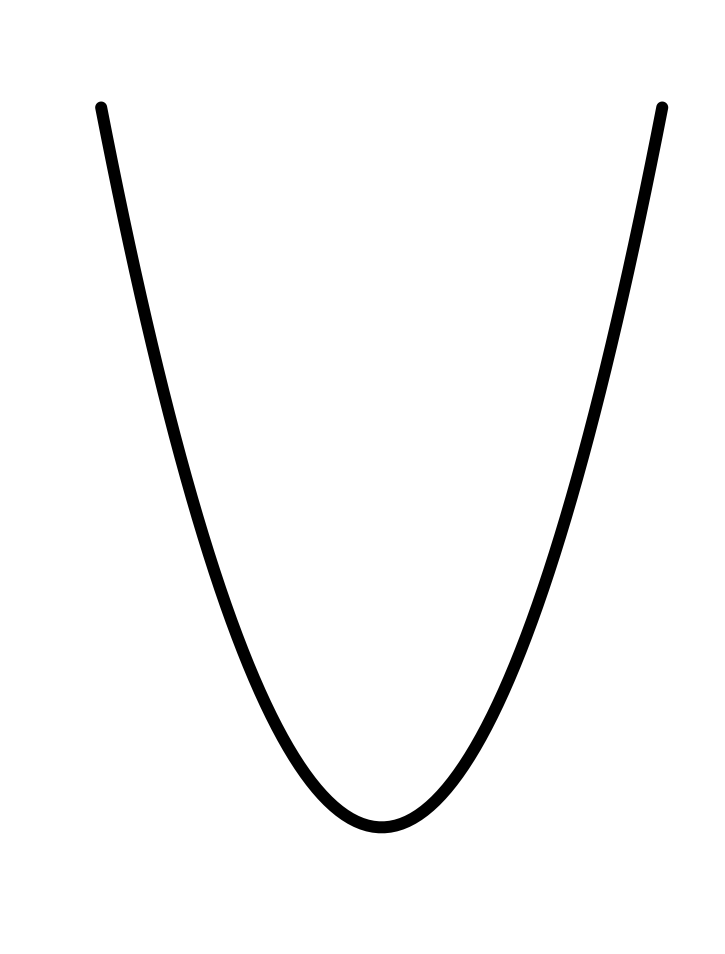
\includegraphics{Preliminaries/www/pb-square.png} &
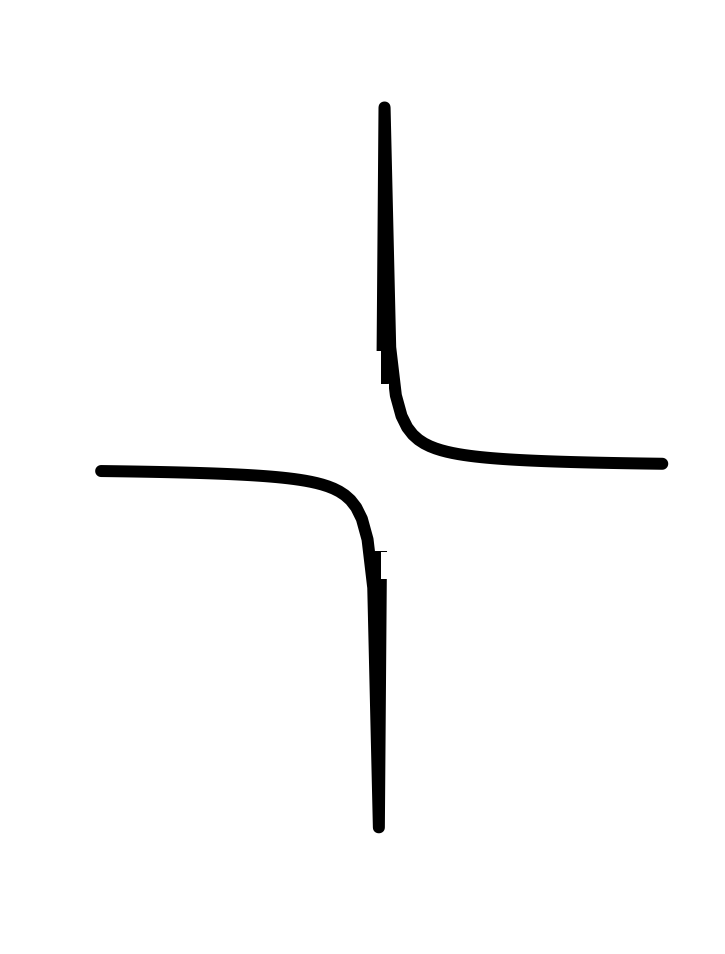
\includegraphics{Preliminaries/www/pb-recip.png} &
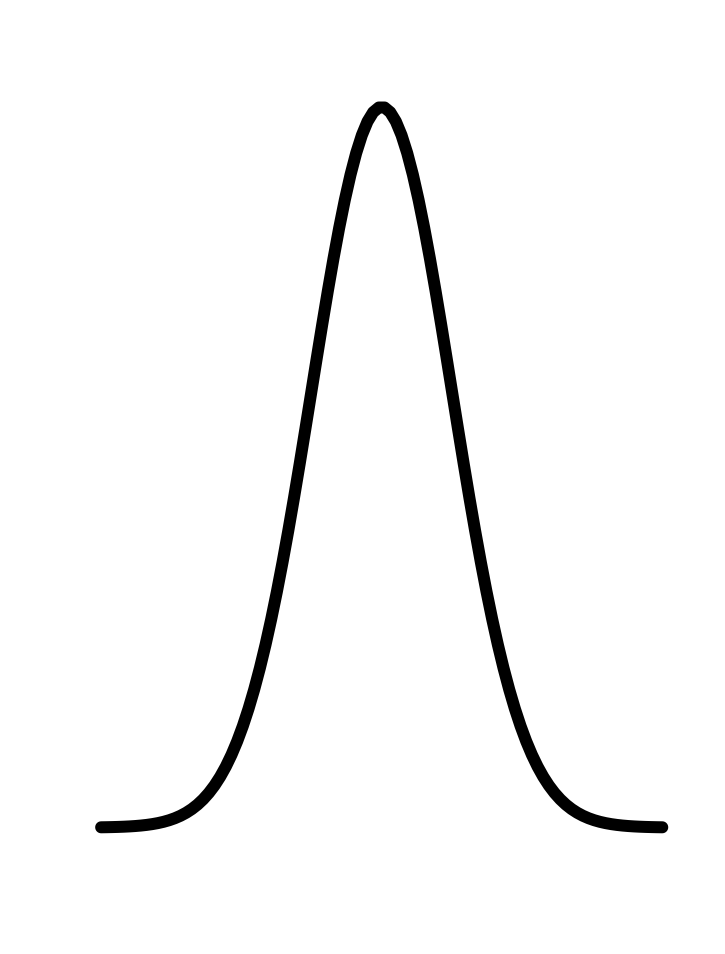
\includegraphics{Preliminaries/www/pb-gauss.png} & & & & \\
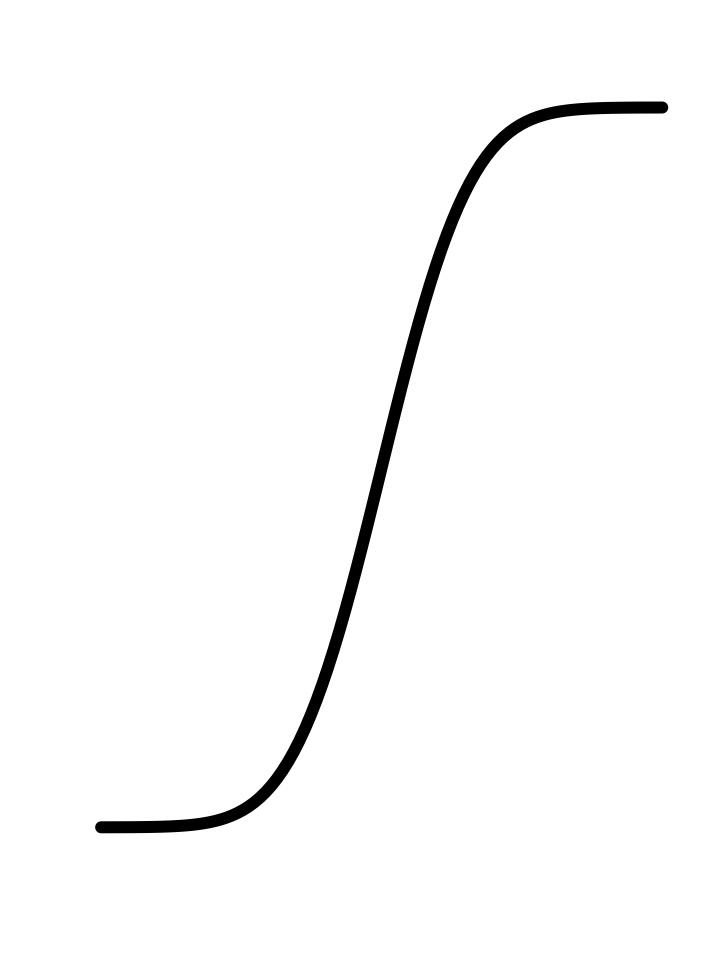
\includegraphics{Preliminaries/www/pb-sigmoid.png} &
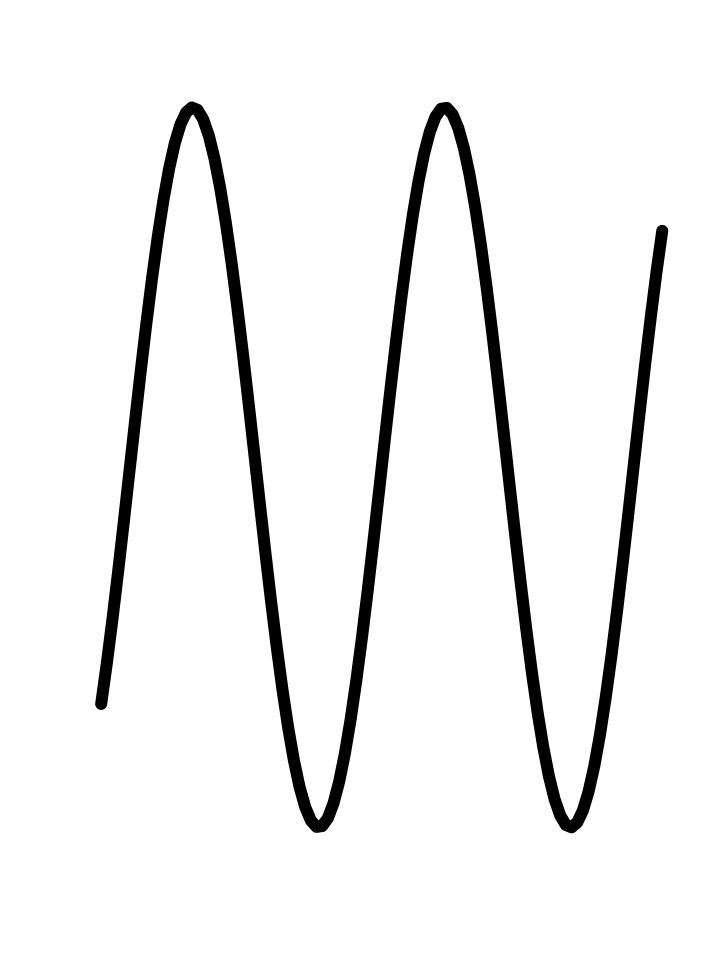
\includegraphics{Preliminaries/www/pb-sin.png} &
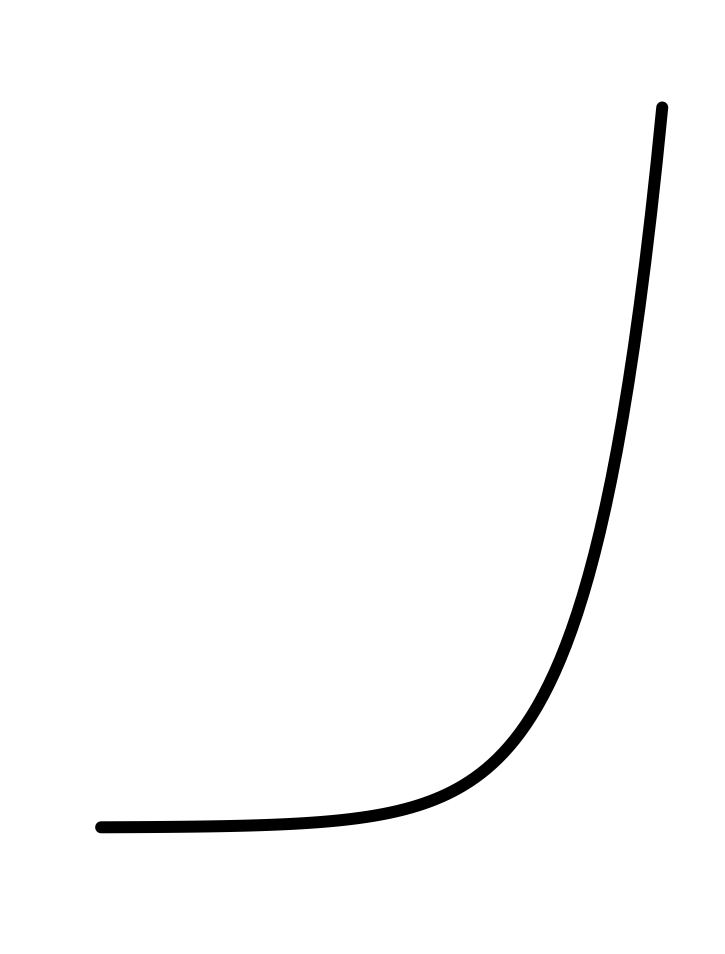
\includegraphics{Preliminaries/www/pb-exp.png} &
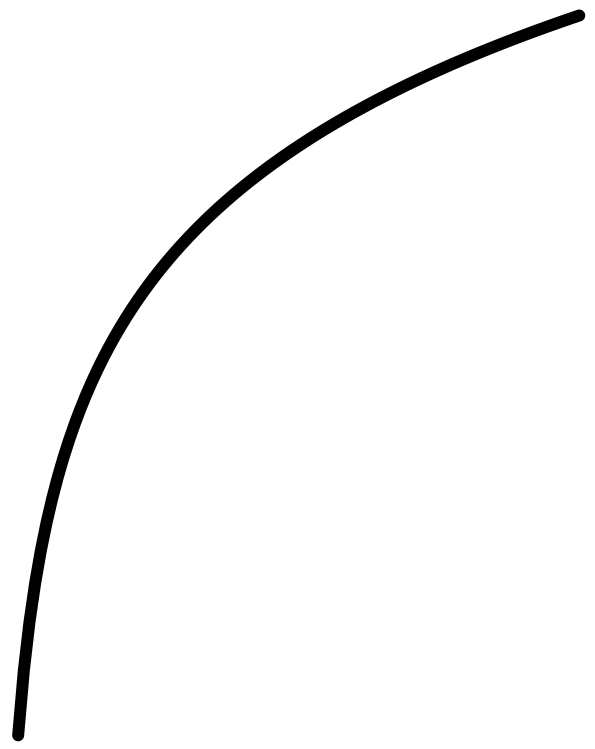
\includegraphics{Preliminaries/www/pb-log.png} & & & & \\
\textbf{sigmoid} & \textbf{sinusoid} & \textbf{exp} & \textbf{ln} & & &
& \\
\bottomrule()
\end{longtable}

}

\end{minipage}%
\newline
\begin{minipage}[t]{\linewidth}

{\centering 

\begin{enumerate}
\def\labelenumi{\arabic{enumi}.}
\item
  Identify which of the eight shapes will remain unaltered even when
  flipped left-to-right.
\item
  Identify which of the eight shapes will remain unaltered if flipped
  left-to-right followed by a top-to-bottom flip.
\item
  Identify which of the eight shapes will give the same result when
  flipped left-to-right or top-to-bottom (but not both!).
\item
  Compare the left-to-right then top-to-bottom flipped exponential to
  the logarithm function. Is the doubly flipped exponential equivalent
  to the logarithm? Explain your reasoning.
\end{enumerate}

}

\end{minipage}%
\newline
\begin{minipage}[t]{\linewidth}

{\centering 

\hypertarget{exer.-11.4}{%
\section*{Exer. 11.4}\label{exer.-11.4}}
\addcontentsline{toc}{section}{Exer. 11.4}

\textbf{Exercise 11.4} ../Modeling/Exercises/spider-tear-plant.Rmd

}

\end{minipage}%
\newline
\begin{minipage}[t]{\linewidth}

{\centering 

Auckland, New Zealand is in a field of dormant volcanos. The highest, at
193 meters above sea level, is
\href{https://en.wikipedia.org/wiki/Maungawhau_/_Mount_Eden}{Maungawhau}.
Formerly, tourists could drive to the peak and look down into the
crater, as seen in the picture.

}

\end{minipage}%
\newline
\begin{minipage}[t]{\linewidth}

{\centering 

\begin{verbatim}
Warning in normalizePath("www/800px-Mt_Eden_Panorama_December_2012.jpg"):
path[1]="www/800px-Mt_Eden_Panorama_December_2012.jpg": No such file or
directory
\end{verbatim}

\begin{figure}

{\centering 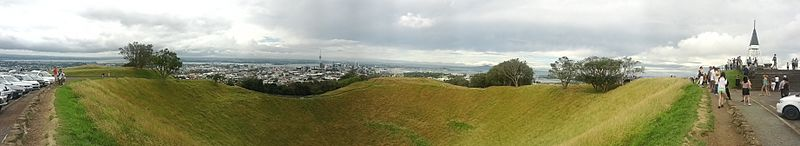
\includegraphics{Preliminaries/www/800px-Mt_Eden_Panorama_December_2012.jpg}

}

\caption{\label{fig-Maungawhau}The crater of Maungawhau, near Auckland,
New Zealand.
\href{https://commons.wikimedia.org/wiki/File:Mt._Eden_Panorama_December_2012.jpg}{Source}}

\end{figure}

}

\end{minipage}%
\newline
\begin{minipage}[t]{\linewidth}

{\centering 

The initial creator of R, Ross Ihaka, teaches at the University of
Auckland. His digitization of a topographic map is easily plotted, as
here:

}

\end{minipage}%
\newline
\begin{minipage}[t]{\linewidth}

{\centering 

\begin{figure}

{\centering 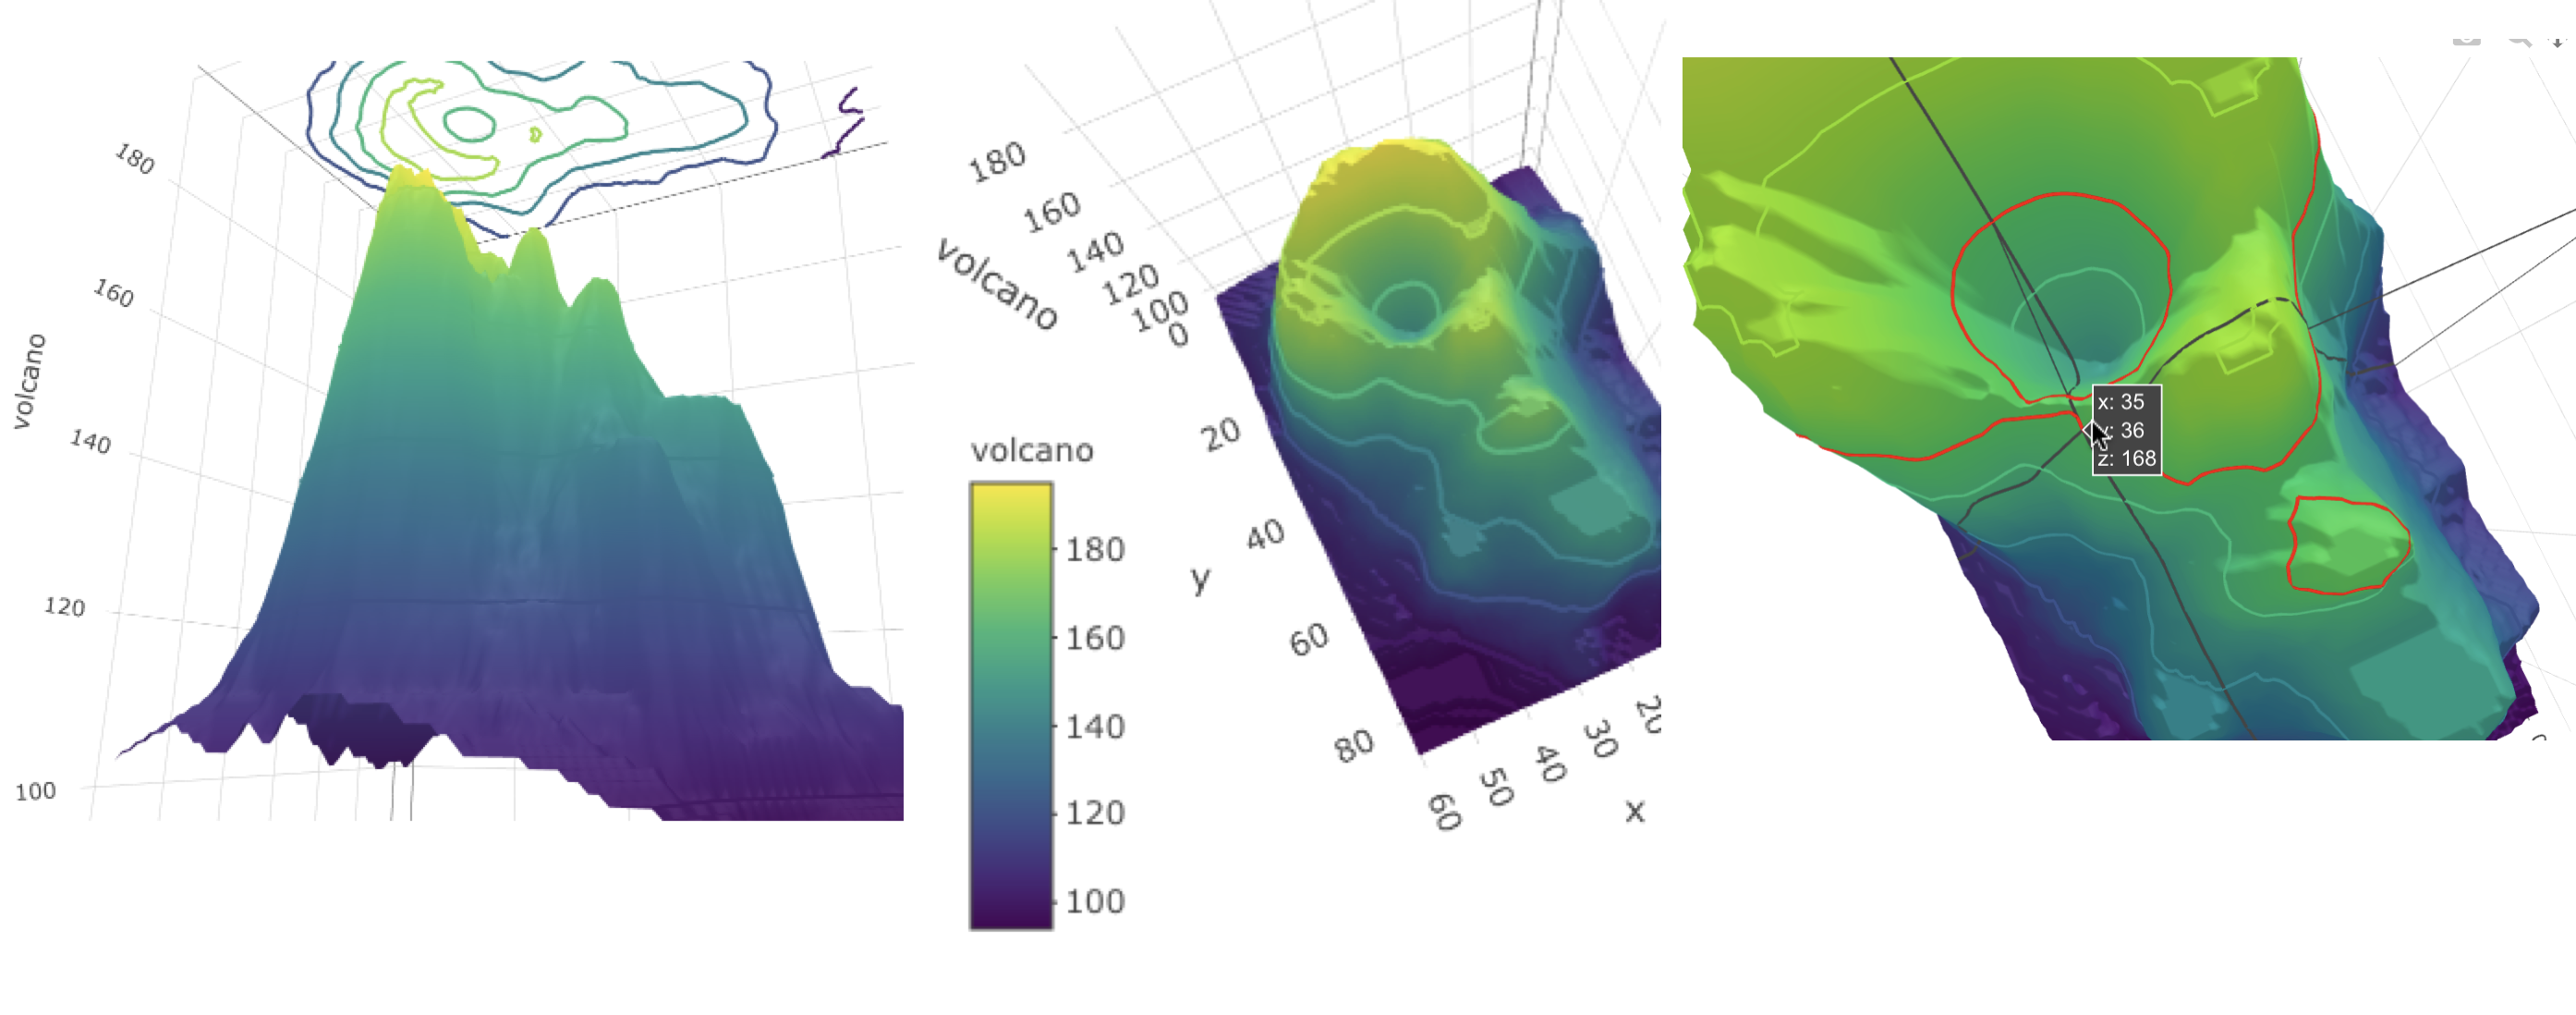
\includegraphics{Preliminaries/www/volcano-multi-view.png}

}

\caption{\label{fig-Maungawhau-plot}A combination surface and contour
plot of the topography of Maungawhau.}

\end{figure}

}

\end{minipage}%
\newline
\begin{minipage}[t]{\linewidth}

{\centering 

The z-axis is height and is in meters. The x- and y-axes are latitude
and longitude, measured in 10-meter units from a reference point. (So,
\(x=10\) is 100 meters from \(x=20\).)

}

\end{minipage}%
\newline
\begin{minipage}[t]{\linewidth}

{\centering 

Get used to the presentation of the surface plot and how to rotate it
and zoom in. To see the crater clearly, you can rotate the surface plot
to look straight downwards, effectively presenting you with a
color-coded contour plot. Moving the cursor over the surface will
display the \(x\) and \(y\) coordinates, as well as the \(z\)-value at
that coordinate point.

}

\end{minipage}%
\newline
\begin{minipage}[t]{\linewidth}

{\centering 

\textbf{Question A} What is the \((x, y)\) location of the low-point of
the crater? (Choose the closest answer.)

~~~~{\((x=34, y=29)\){\(\heartsuit\ \)}}~~~~~~~{\((x=31, y=25)\){︎X
}}~~~~~~~{\((x=25, y=34)\){x}}~~~~~~~{\((x=29, y=34)\){x}}

}

\end{minipage}%
\newline
\begin{minipage}[t]{\linewidth}

{\centering 

\textbf{Question B} What color is used to designate the \textbf{lowest}
elevations?

~~~~{dark blue{\(\heartsuit\ \)}}~~~~~~~{green{x}}~~~~~~~{yellow{x}}

}

\end{minipage}%
\newline
\begin{minipage}[t]{\linewidth}

{\centering 

If you were to climb up Maungawhau, at some point you would be at the
same elevation as the low-point of the crater, even though you are
\emph{outside} the crater. Think of the contour that corresponds to that
elevation. Let's call it the ``half-way'' contour since it's roughly
half-way up the volcano.

}

\end{minipage}%
\newline
\begin{minipage}[t]{\linewidth}

{\centering 

\textbf{Question C} What is the shape of the ``half-way'' contour?

~~~~{a line segment{x}}~~~~~~~{a crescent{x}}~~~~~~~{a closed
curve{\(\heartsuit\ \)}}~~~~~~~{a cross{x}}

}

\end{minipage}%
\newline
\begin{minipage}[t]{\linewidth}

{\centering 

Imagine that you are filling up the crater with water. At some point,
the water rises to a level where it will spill over the lip of the
crater.

}

\end{minipage}%
\newline
\begin{minipage}[t]{\linewidth}

{\centering 

\textbf{Question D} What is the elevation at which the water will start
to spill over the crater lip? (Pick the closest answer.)

~~~~{169 meters{\(\heartsuit\ \)}}~~~~~~~{172 meters{x}}~~~~~~~{175
meters{x}}~~~~~~~{178 meters{x}}

}

\end{minipage}%
\newline
\begin{minipage}[t]{\linewidth}

{\centering 

\textbf{Question E} Explain in terms of the shapes of contours how you
can identify the elevation at which the water would spill over the rim.

}

\end{minipage}%
\newline
\begin{minipage}[t]{\linewidth}

{\centering 

\hypertarget{exer.-11.5}{%
\section*{Exer. 11.5}\label{exer.-11.5}}
\addcontentsline{toc}{section}{Exer. 11.5}

\textbf{Exercise 11.5} ../Modeling/Exercises/drawing.Rmd

}

\end{minipage}%
\newline
\begin{minipage}[t]{\linewidth}

{\centering 

We've created a function named \(\text{twins}(x,y)\) to help you
practice making contour plots. You'll need to open a sandbox to draw the
plot.

}

\end{minipage}%
\newline
\begin{minipage}[t]{\linewidth}

{\centering 

Here is some scaffolding for the command:

}

\end{minipage}%
\newline
\begin{minipage}[t]{\linewidth}

{\centering 

\begin{Shaded}
\begin{Highlighting}[]
\NormalTok{twins }\OtherTok{\textless{}{-}}\NormalTok{ mosaic}\SpecialCharTok{::}\FunctionTok{rfun}\NormalTok{(}\SpecialCharTok{\textasciitilde{}}\NormalTok{ x }\SpecialCharTok{+}\NormalTok{ y, }\AttributeTok{seed =} \DecValTok{302}\NormalTok{, }\AttributeTok{n=}\DecValTok{5}\NormalTok{)}
\FunctionTok{contour\_plot}\NormalTok{(}\FunctionTok{twins}\NormalTok{(x, y) }\SpecialCharTok{\textasciitilde{}}\NormalTok{ x }\SpecialCharTok{+}\NormalTok{ y, }\FunctionTok{domain}\NormalTok{(}\AttributeTok{x=}\FunctionTok{c}\NormalTok{(}\DecValTok{0}\NormalTok{,}\DecValTok{1}\NormalTok{), }\AttributeTok{y=}\FunctionTok{c}\NormalTok{(}\SpecialCharTok{{-}}\DecValTok{1}\NormalTok{,}\DecValTok{1}\NormalTok{)))}
\end{Highlighting}
\end{Shaded}

\begin{figure}[H]

{\centering \includegraphics{Preliminaries/exercise-layout_files/figure-pdf/unnamed-chunk-89-1.pdf}

}

\end{figure}

}

\end{minipage}%
\newline
\begin{minipage}[t]{\linewidth}

{\centering 

\textbf{Question A} The domain of the plot should be large enough to
show a mountain next to a deep hole. Which of these domains will do the
job?

\begin{enumerate}
\def\labelenumi{\roman{enumi}.}
\tightlist
\item
  {\texttt{domain(x=c(-5,\ 5),\ y=c(-5,\ 5)}{Right!~}}\\
\item
  {\texttt{domain(x=c(1,\ 5),\ y=c(1,\ 5)}{xThis shows the mountain,
  but not the hole.}}\\
\item
  {\texttt{domain(x=c(1,1),\ y=c(-1,1)))}{xSome of the hole is shown,
  but none of the mountain.}}\\
\item
  {\texttt{domain(x=c(5,10),\ y=c(0,10)))}{xThere's hardly anything
  going on in this domain. The function here is pretty flat except for a
  dip in the lower left.}}
\end{enumerate}

}

\end{minipage}%
\newline
\begin{minipage}[t]{\linewidth}

{\centering 

In a different sandbox (so you can still see the contour plot in the
first sandbox), draw a \textbf{slice} through the function along the
line \(y=0\). Use the same \(x\)-domain as in the correct answer to the
previous question.

}

\end{minipage}%
\newline
\begin{minipage}[t]{\linewidth}

{\centering 

In the \texttt{slice\_plot()} command below, you will need to replace
\texttt{\_\_tilde-expression\_\_\_} and \texttt{\_\_domain\_\_} with the
correct syntax.

}

\end{minipage}%
\newline
\begin{minipage}[t]{\linewidth}

{\centering 

\begin{Shaded}
\begin{Highlighting}[]
\NormalTok{twins }\OtherTok{\textless{}{-}}\NormalTok{ mosaic}\SpecialCharTok{::}\FunctionTok{rfun}\NormalTok{(}\SpecialCharTok{\textasciitilde{}}\NormalTok{ x }\SpecialCharTok{+}\NormalTok{ y, }\AttributeTok{seed =} \DecValTok{302}\NormalTok{, }\AttributeTok{n=}\DecValTok{5}\NormalTok{)}
\FunctionTok{slice\_plot}\NormalTok{(\_\_tilde}\SpecialCharTok{{-}}\NormalTok{expression\_\_, \_\_domain\_\_)}
\end{Highlighting}
\end{Shaded}

}

\end{minipage}%
\newline
\begin{minipage}[t]{\linewidth}

{\centering 

\textbf{Question B} Which of these expressions will accomplish the task?

\begin{enumerate}
\def\labelenumi{\roman{enumi}.}
\tightlist
\item
  {\texttt{slice\_plot(twins(x,\ y=0)\ \textasciitilde{}\ x,\ domain(x=c(-5,5)))}{Excellent!~}}\\
\item
  {\texttt{slice\_plot(twins(x)\ \textasciitilde{}\ x,\ domain(y=c(-5,\ 5)))}{︎X
  The domain should be over \(x\), not \(y\). And \texttt{twins()} takes
  two inputs, even if one of them is fixed at zero.}}\\
\item
  {\texttt{slice\_plot(twins(x,\ y=0)\ \textasciitilde{}\ x,\ domain(x=c(-5,\ 5),\ y=c(-5,\ 5)))}{︎X
  A slice plot has a domain that includes only one input.}}\\
\item
  {\texttt{slice\_plot(twins(x,\ y=0)\ \textasciitilde{}\ x\ +\ y,\ domain(x=c(-5,\ 5),\ y=c(-5,\ 5)))}{︎X
  A slice plot has only one input on the right side of the tilde
  expression.}}
\end{enumerate}

}

\end{minipage}%
\newline
\begin{minipage}[t]{\linewidth}

{\centering 

\hypertarget{exer.-11.7}{%
\section*{Exer. 11.7}\label{exer.-11.7}}
\addcontentsline{toc}{section}{Exer. 11.7}

\textbf{Exercise 11.7} ../Modeling/Exercises/duck-see-socks.Rmd

}

\end{minipage}%
\newline
\begin{minipage}[t]{\linewidth}

{\centering 

PICK UP ON THIS IN ACCUMULATION BLOCK TO calculate the Gini Coefficient.

}

\end{minipage}%
\newline
\begin{minipage}[t]{\linewidth}

{\centering 

Income inequality is a matter of perennial political debate. In the US,
most people support Social Security, which is an income re-distribution
programming dating back almost a century. But other re-distribution
policies are controversial. Some believe they are essential to a healthy
society, others that the ``cure'' is worse than the ``disease.''

}

\end{minipage}%
\newline
\begin{minipage}[t]{\linewidth}

{\centering 

Whatever one's views, it's helpful to have a way to quantify inequality.
There are many ways that this might be done. A mathematically
sophisticated one is called the \textbf{\emph{Gini coefficient}}.

}

\end{minipage}%
\newline
\begin{minipage}[t]{\linewidth}

{\centering 

Imagine that society was divided statistically into income groups, from
poorest to richest. Each of these income groups consists of a fraction
of the population and has, in aggregate, a fraction of the national
income. Poor people tend to be many in number but to have a very small
fraction of income. Wealthy people are few in number, but have a large
fraction of income. The table shows data for US households in
2009:\sidenote{\footnotesize These data, as well as the general idea for the topic
  come from La Haye and Zizler (2021), ``The Lorenz Curve in the
  Classroom'', \emph{The American Statistician}, 75(2):217-225}

}

\end{minipage}%
\newline
\begin{minipage}[t]{\linewidth}

{\centering 

\begin{longtable}[]{@{}lrrl@{}}
\toprule()
group label & population & aggregate income & cumulative income \\
\midrule()
\endhead
poorest & 20\% & 3.4\% & 3.4\% \\
low-middle & 20\% & 8.6\% & 12.0\% \\
middle & 20\% & 14.6\% & 26.6\% \\
high-middle & 20\% & 23.2\% & 47.8\% \\
richest & 20\% & 50.2\% & 100.0\% \\
\bottomrule()
\end{longtable}

}

\end{minipage}%
\newline
\begin{minipage}[t]{\linewidth}

{\centering 

The \textbf{\emph{cumulative}} income shows the fraction of income of
all the people in that group or poorer. The cumulative population adds
up the population fraction in that row and previous rows. So, a
cumulative population of 60\% means ``the poorest 60\% of the
population'' which, as the table shows, earn as a group 14.6\% of the
total income for the whole population.

}

\end{minipage}%
\newline
\begin{minipage}[t]{\linewidth}

{\centering 

A function that relates the cumulative population to the cumulative
income is called a \textbf{\emph{Lorenz function}}. The data are graphed
in Figure~\ref{fig-lorenz-data} and available as the \texttt{US\_income}
data frame in the SANDBOX. Later, in Figure~\ref{fig-lorenz-one-fun},
we'll fit parameterized functions to the data.

}

\end{minipage}%
\newline
\begin{minipage}[t]{\linewidth}

{\centering 

\begin{figure}

\sidecaption{\label{fig-lorenz-data}Data on household incomes in the US
in 2009.}

{\centering 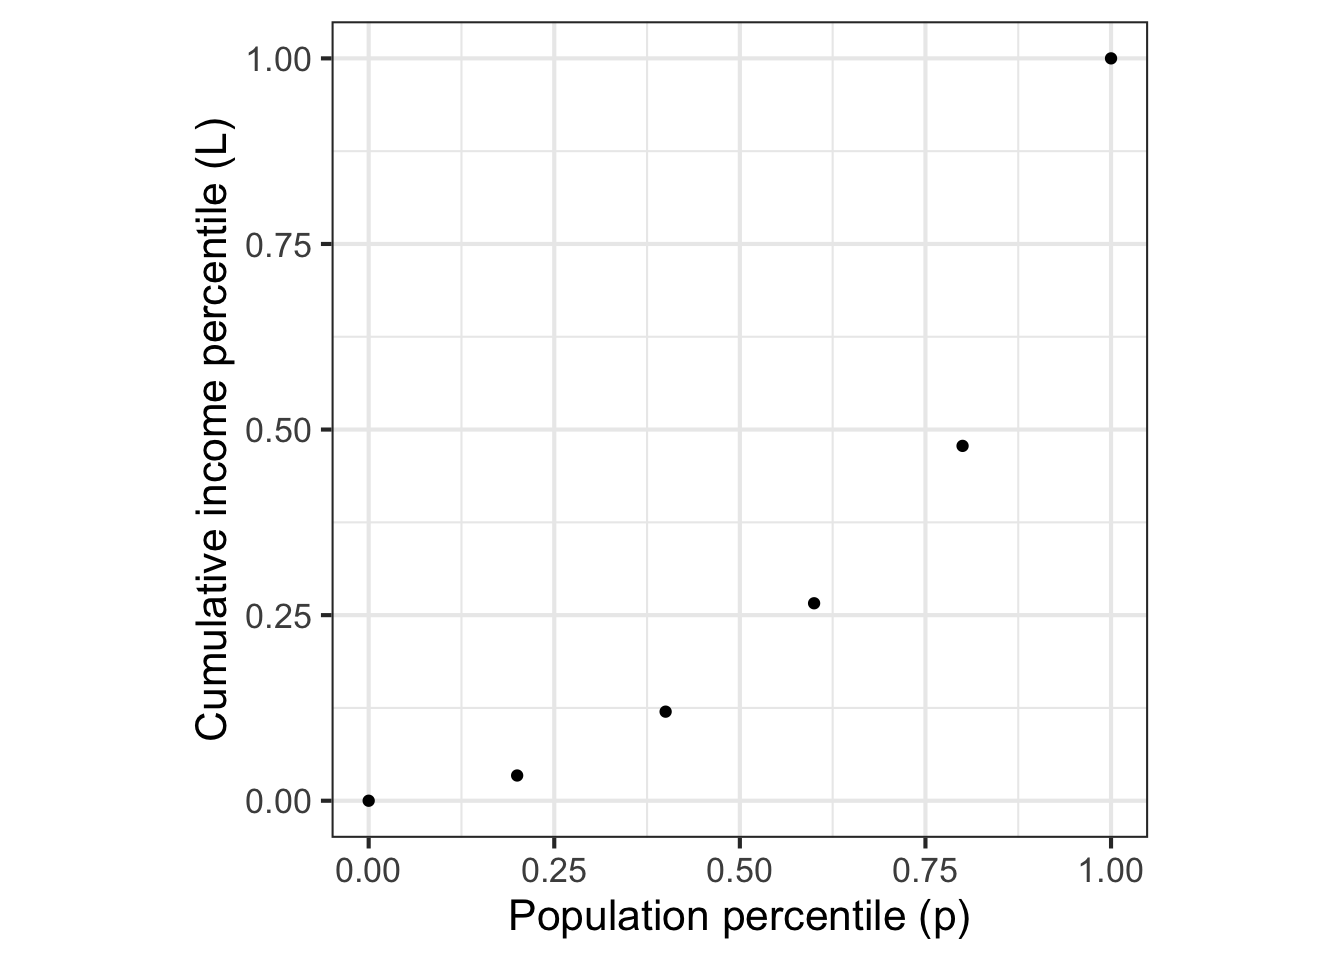
\includegraphics{Preliminaries/exercise-layout_files/figure-pdf/fig-lorenz-data-1.pdf}

}

\end{figure}

}

\end{minipage}%
\newline
\begin{minipage}[t]{\linewidth}

{\centering 

Lorenz curves must:

}

\end{minipage}%
\newline
\begin{minipage}[t]{\linewidth}

{\centering 

\begin{itemize}
\tightlist
\item
  Be concave up, which amounts to saying that the curve gets steeper and
  steeper as the population percentile increases. (Why? Because at any
  point, poorer people are to the left and richer to the right.)
\item
  Connect (0,0) to (1, 1).
\end{itemize}

}

\end{minipage}%
\newline
\begin{minipage}[t]{\linewidth}

{\centering 

Calling the income percentile \(L\) a function of the population
percentile \(p\), a Lorenz function is \(L(p)\) that satisfies the
requirements in the previous paragraph. Here are some functions that
meet the requirements:

}

\end{minipage}%
\newline
\begin{minipage}[t]{\linewidth}

{\centering 

\begin{itemize}
\tightlist
\item
  \(L_b(p) \equiv p^b\) where \(1 \leq b\).
\item
  \(L_q(p) \equiv 1 - (1-p)^q\) where \(0 < q \leq 1\)
\end{itemize}

}

\end{minipage}%
\newline
\begin{minipage}[t]{\linewidth}

{\centering 

Notice that each of these functions has just one parameter. It seems
implausible that the workings of a complex society can be summarized
with just one number. We can use the curve-polishing techniques that
will be introduced in
(\textbf{chap-fitting-polishing?})\marginpar{\begin{footnotesize}{?quarto-cite:chap-fitting-polishing}\vspace{2mm}\par\end{footnotesize}}
to find the ``best'' parameter value to match the data.

}

\end{minipage}%
\newline
\begin{minipage}[t]{\linewidth}

{\centering 

\begin{Shaded}
\begin{Highlighting}[]
\NormalTok{Lb }\OtherTok{\textless{}{-}} \FunctionTok{fitModel}\NormalTok{(income }\SpecialCharTok{\textasciitilde{}}\NormalTok{ pop}\SpecialCharTok{\^{}}\NormalTok{b, }\AttributeTok{data =}\NormalTok{ Income, }\AttributeTok{start=}\FunctionTok{list}\NormalTok{(}\AttributeTok{b=}\FloatTok{1.5}\NormalTok{))}
\NormalTok{Lq }\OtherTok{\textless{}{-}} \FunctionTok{fitModel}\NormalTok{(income }\SpecialCharTok{\textasciitilde{}} \DecValTok{1} \SpecialCharTok{{-}}\NormalTok{ (}\DecValTok{1}\SpecialCharTok{{-}}\NormalTok{pop)}\SpecialCharTok{\^{}}\NormalTok{q, }\AttributeTok{data =}\NormalTok{ Income, }\AttributeTok{start=}\FunctionTok{list}\NormalTok{(}\AttributeTok{q=}\FloatTok{0.5}\NormalTok{))}
\end{Highlighting}
\end{Shaded}

}

\end{minipage}%
\newline
\begin{minipage}[t]{\linewidth}

{\centering 

Figure~\ref{fig-lorenz-one-fun} compares the fitted functions to the
data.

}

\end{minipage}%
\newline
\begin{minipage}[t]{\linewidth}

{\centering 

\begin{figure}

\sidecaption{\label{fig-lorenz-one-fun}Lorenz curves \(L_b(p)\) (blue)
and \(L_q(p)\) (magenta) fitted to the household income data.}

{\centering 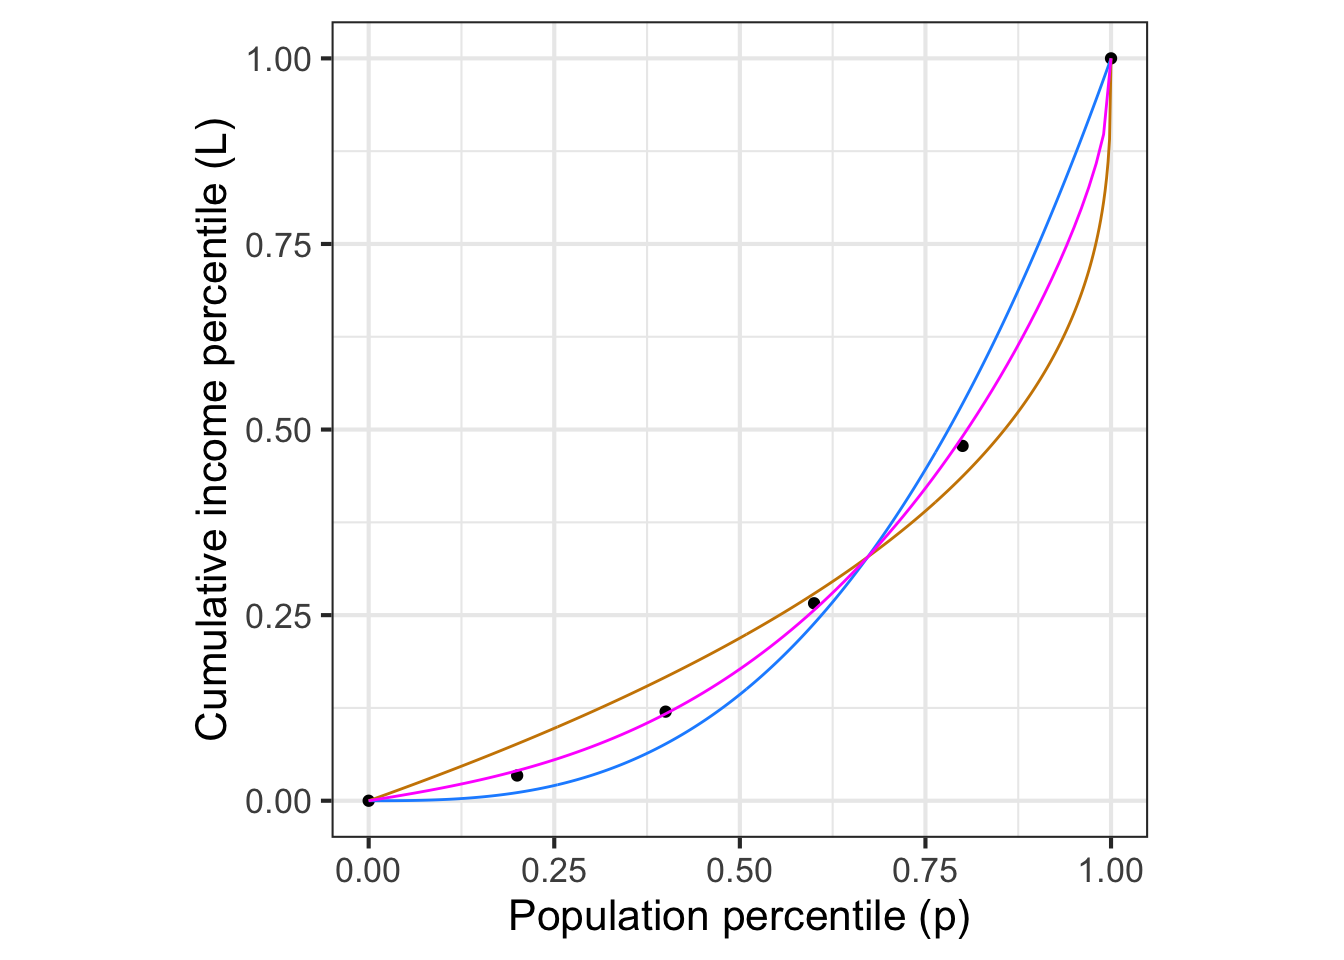
\includegraphics{Preliminaries/exercise-layout_files/figure-pdf/fig-lorenz-one-fun-1.pdf}

}

\end{figure}

}

\end{minipage}%
\newline
\begin{minipage}[t]{\linewidth}

{\centering 

Neither form \(L_b(p)\) or \(L_q(p)\) gives a compelling description of
the data. Where should we go from here?

}

\end{minipage}%
\newline
\begin{minipage}[t]{\linewidth}

{\centering 

We can provide more parameters by constructing more complicated Lorenz
functions. Here are two ways to build a new Lorenz function out of an
existing one:

}

\end{minipage}%
\newline
\begin{minipage}[t]{\linewidth}

{\centering 

\begin{itemize}
\tightlist
\item
  The product of any two Lorenz functions, \(L_1(p) L_2(p)\) is itself a
  Lorenz function.
\item
  A linear combination of any two Lorenz functions,
  \(a L_1(p) + (1-a) L_2(p)\), so long as the scalars add up to 1, is
  itself a Lorenz function. For instance, the magenta curve in
  Figure~\ref{fig-lorenz-one-fun} is the linear combination of 0.45
  times the tan curve plus 0.55 times the blue curve.
\end{itemize}

}

\end{minipage}%
\newline
\begin{minipage}[t]{\linewidth}

{\centering 

Question: Is the composition of two Lorenz functions a Lorenz function?
That is, does the composition meet the two requirements for being a
Lorenz function?

}

\end{minipage}%
\newline
\begin{minipage}[t]{\linewidth}

{\centering 

To get started, figure out whether or not \(L_1(L_2(0)) = 0\) and
\(L_1(L_2(1)) = 1\). If the answer is yes, then we need to find a way to
compute the concavity of a Lorenz function to determine if the
composition will always be concave up. We'll need additional tools for
this. We'll introduce these in Block 2.

}

\end{minipage}%
\newline
\begin{minipage}[t]{\linewidth}

{\centering 

\hypertarget{exer.-11.8}{%
\section*{Exer. 11.8}\label{exer.-11.8}}
\addcontentsline{toc}{section}{Exer. 11.8}

\textbf{Exercise 11.8} ../Modeling/Exercises/kid-type-boat.Rmd

}

\end{minipage}%
\newline
\begin{minipage}[t]{\linewidth}

{\centering 

These three expressions

}

\end{minipage}%
\newline
\begin{minipage}[t]{\linewidth}

{\centering 

\[e^{kt}\ \ \ \ \ 10^{t/d} \  \ \ \ \  2^{t/h}\]

}

\end{minipage}%
\newline
\begin{minipage}[t]{\linewidth}

{\centering 

produce the same value if \(k\), \(d\) and \(h\) have corresponding
numerical values.

}

\end{minipage}%
\newline
\begin{minipage}[t]{\linewidth}

{\centering 

The scaffolding has an expression for plotting out \(2^{t/h}\) for
\(-4 \leq t \leq 12\) where \(h = 4\). It also plots out \(e^{kt}\) and
\(10^{t/d}\)

\begin{Shaded}
\begin{Highlighting}[]
\NormalTok{fa }\OtherTok{\textless{}{-}} \FunctionTok{makeFun}\NormalTok{(}\FunctionTok{exp}\NormalTok{(k}\SpecialCharTok{*}\NormalTok{t)  }\SpecialCharTok{\textasciitilde{}}\NormalTok{ t, }\AttributeTok{k =} \DecValTok{4}\NormalTok{)}
\NormalTok{fc }\OtherTok{\textless{}{-}} \FunctionTok{makeFun}\NormalTok{(}\DecValTok{2}\SpecialCharTok{\^{}}\NormalTok{(t}\SpecialCharTok{/}\NormalTok{h) }\SpecialCharTok{\textasciitilde{}}\NormalTok{ t, }\AttributeTok{h =} \DecValTok{4}\NormalTok{)}
\NormalTok{fb }\OtherTok{\textless{}{-}} \FunctionTok{makeFun}\NormalTok{(}\DecValTok{10}\SpecialCharTok{\^{}}\NormalTok{(t}\SpecialCharTok{/}\NormalTok{d) }\SpecialCharTok{\textasciitilde{}}\NormalTok{ t, }\AttributeTok{d =} \DecValTok{4}\NormalTok{)}

\FunctionTok{slice\_plot}\NormalTok{(}\FunctionTok{fa}\NormalTok{(t) }\SpecialCharTok{\textasciitilde{}}\NormalTok{ t, }\FunctionTok{domain}\NormalTok{(}\AttributeTok{t =} \FunctionTok{c}\NormalTok{(}\SpecialCharTok{{-}}\DecValTok{4}\NormalTok{, }\DecValTok{12}\NormalTok{))) }\SpecialCharTok{\%\textgreater{}\%}
  \FunctionTok{slice\_plot}\NormalTok{(}\FunctionTok{fb}\NormalTok{(t) }\SpecialCharTok{\textasciitilde{}}\NormalTok{ t, }\AttributeTok{color=}\StringTok{"blue"}\NormalTok{) }\SpecialCharTok{\%\textgreater{}\%}
  \FunctionTok{slice\_plot}\NormalTok{(}\FunctionTok{fc}\NormalTok{(t) }\SpecialCharTok{\textasciitilde{}}\NormalTok{ t, }\AttributeTok{color  =} \StringTok{"red"}\NormalTok{) }\SpecialCharTok{\%\textgreater{}\%}
  \FunctionTok{gf\_lims}\NormalTok{(}\AttributeTok{y =} \FunctionTok{c}\NormalTok{(}\DecValTok{0}\NormalTok{, }\DecValTok{8}\NormalTok{))}
\end{Highlighting}
\end{Shaded}

}

\end{minipage}%
\newline
\begin{minipage}[t]{\linewidth}

{\centering 

Your task is to modify the values of \texttt{d} and \texttt{k} such that
all three curves lie on top of one another. (Leave \texttt{h} at the
value 4.) You can find the appropriate values of \texttt{d} and
\texttt{k} to accomplish this by any means you like, say, by using the
algebra of exponents or by using trial and error. (Trial and error is a
perfectly valid strategy regardless of what your high-school math
teachers might have said about ``guess and check.'' The trick is to make
each new guess systematically based on your previous ones and
observation of how those previous ones performed.)

}

\end{minipage}%
\newline
\begin{minipage}[t]{\linewidth}

{\centering 

After you have found values of \texttt{k} and \texttt{d} that are suited
to the task \ldots{}

}

\end{minipage}%
\newline
\begin{minipage}[t]{\linewidth}

{\centering 

\textbf{Question A} What is the numerical value of your best estimate of
\texttt{k}?

~~~~{0.143{x}}~~~~~~~{0.173{\(\heartsuit\ \)}}~~~~~~~{0.283{︎X
}}~~~~~~~{0.320{x}}

}

\end{minipage}%
\newline
\begin{minipage}[t]{\linewidth}

{\centering 

\textbf{Question B} What is the numerical value of your best estimate of
\texttt{d}?

~~~~{11.2{x}}~~~~~~~{11.9{︎X
}}~~~~~~~{13.3{\(\heartsuit\ \)}}~~~~~~~{15.8{x}}

}

\end{minipage}%
\newline
\begin{minipage}[t]{\linewidth}

{\centering 

\hypertarget{exer.-11.9}{%
\section*{Exer. 11.9}\label{exer.-11.9}}
\addcontentsline{toc}{section}{Exer. 11.9}

\textbf{Exercise 11.9} ../Modeling/Exercises/flipping-1.Rmd

}

\end{minipage}%
\newline
\begin{minipage}[t]{\linewidth}

{\centering 

\begin{figure}

{\centering 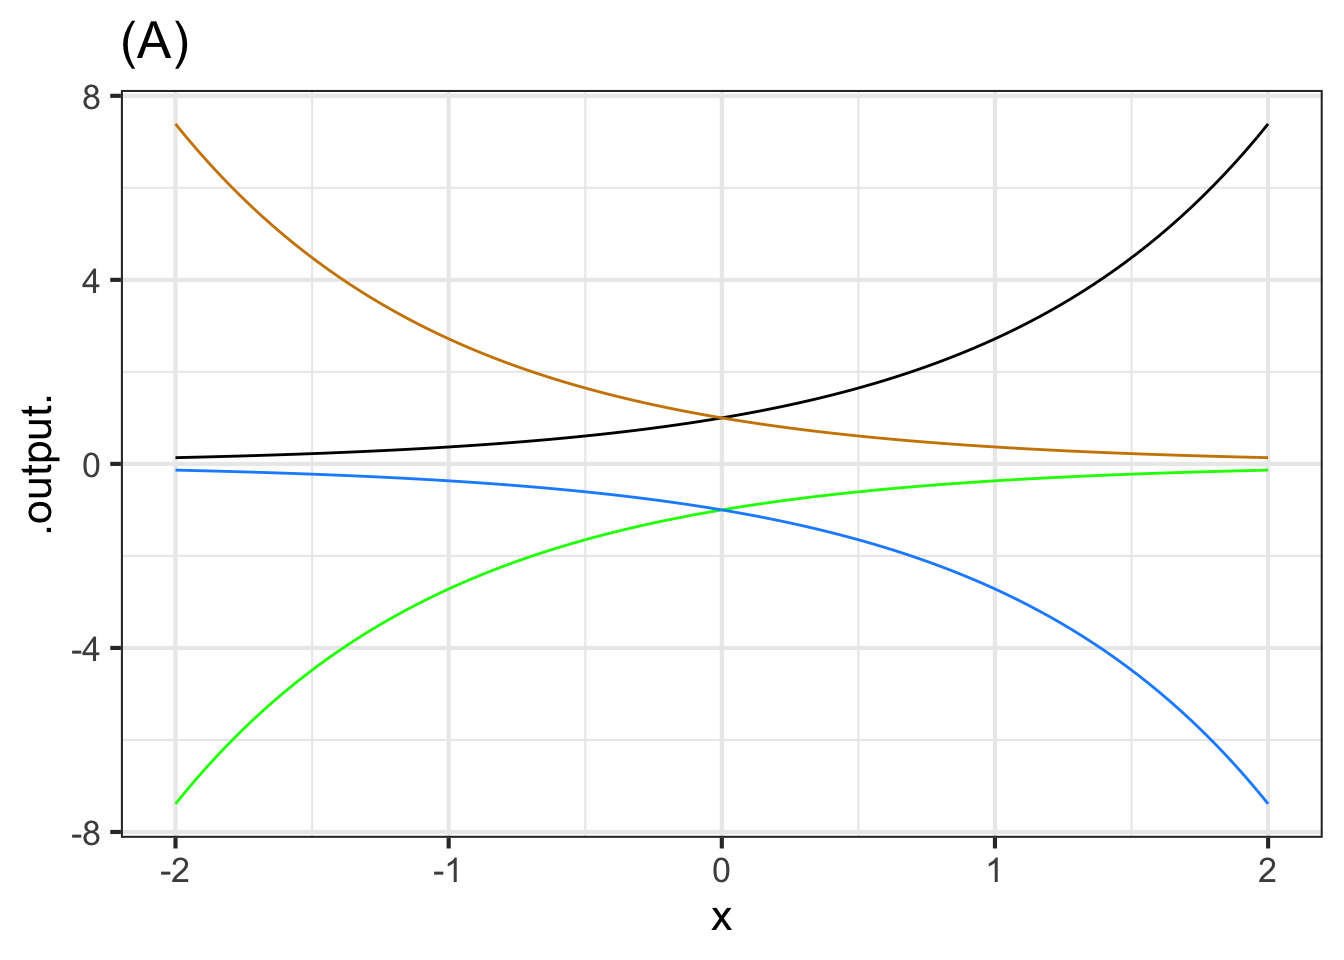
\includegraphics{Preliminaries/exercise-layout_files/figure-pdf/fig-flipping-1-1-1.pdf}

}

\caption{\label{fig-flipping-1-1}\textbf{?(caption)}}

\end{figure}

}

\end{minipage}%
\newline
\begin{minipage}[t]{\linewidth}

{\centering 

\textbf{Question A} One of the curves in plot (A) is a pattern-book
function. Which one?

~~~~{black{\(\heartsuit\ \)It's the exponential
function.}}~~~~~~~{blue{x}}~~~~~~~{green{x}}~~~~~~~{tan{︎X
}}~~~~~~~{none of them{x}}

}

\end{minipage}%
\newline
\begin{minipage}[t]{\linewidth}

{\centering 

\textbf{Question B} Taking \(f()\) to be the pattern-book function in
plot (A), which one of the curves is \(f(-x)\)?

~~~~{black{x}}~~~~~~~{blue{x}}~~~~~~~{green{︎X
}}~~~~~~~{tan{\(\heartsuit\ \)}}~~~~~~~{none of them{x}}

}

\end{minipage}%
\newline
\begin{minipage}[t]{\linewidth}

{\centering 

\begin{figure}

{\centering 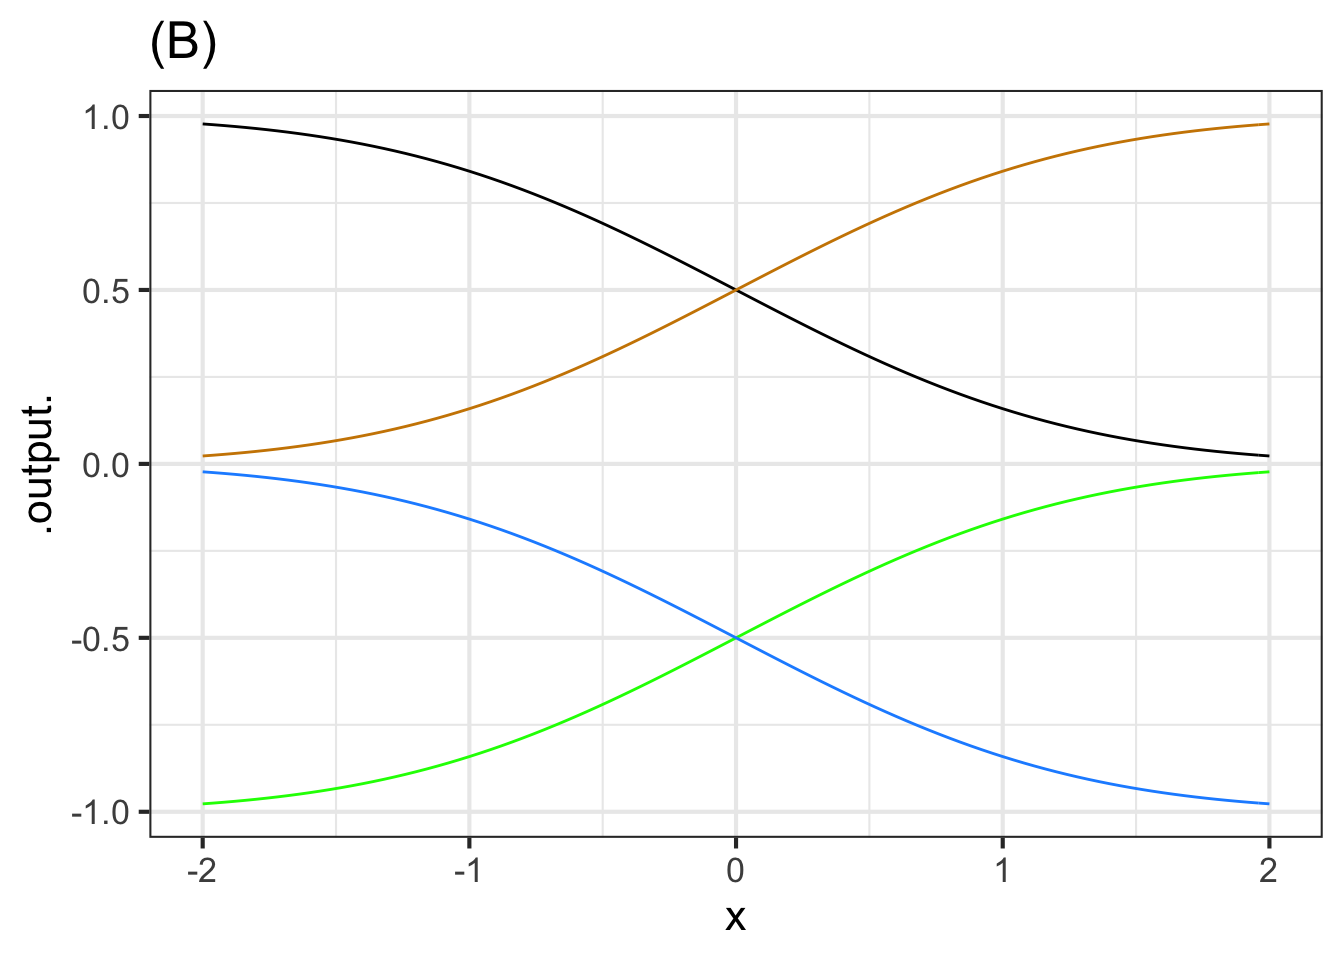
\includegraphics{Preliminaries/exercise-layout_files/figure-pdf/fig-flipping-1-2-1.pdf}

}

\caption{\label{fig-flipping-1-2}\textbf{?(caption)}}

\end{figure}

}

\end{minipage}%
\newline
\begin{minipage}[t]{\linewidth}

{\centering 

\textbf{Question C} One of the curves in plot (B) is a pattern-book
function. Which one?

~~~~{black{x}}~~~~~~~{blue{x}}~~~~~~~{green{︎X
}}~~~~~~~{tan{\(\heartsuit\ \)}}~~~~~~~{none of them{x}}

}

\end{minipage}%
\newline
\begin{minipage}[t]{\linewidth}

{\centering 

\textbf{Question D} Taking \(f()\) to be the pattern-book function in
plot (B), which one of the curves is \(-f(x)\)?

~~~~{black{x}}~~~~~~~{blue{\(\heartsuit\ \)}}~~~~~~~{green{︎X
}}~~~~~~~{tan{x}}~~~~~~~{none of them{x}}

}

\end{minipage}%
\newline
\begin{minipage}[t]{\linewidth}

{\centering 

\begin{figure}

{\centering \includegraphics{Preliminaries/exercise-layout_files/figure-pdf/fig-flipping-1-3-1.pdf}

}

\caption{\label{fig-flipping-1-3}\textbf{?(caption)}}

\end{figure}

}

\end{minipage}%
\newline
\begin{minipage}[t]{\linewidth}

{\centering 

The blue curve in plot (C), as you know, is the sinusoid pattern-book
function.

}

\end{minipage}%
\newline
\begin{minipage}[t]{\linewidth}

{\centering 

\textbf{Question E} Which of these functions is the green curve?

\begin{enumerate}
\def\labelenumi{\roman{enumi}.}
\tightlist
\item
  {\(\sin(-x)\){x}}\\
\item
  {\(-\sin(x)\){x}}\\
\item
  {\(-\sin(-x)\){x}}\\
\item
  {Both \(\sin(-x)\) and \(-\sin(-x)\){x}}\\
\item
  {Both \(\sin(-x)\) and \(-\sin(x)\){Nice!~The sine function has
  so-called ``odd'' symmetry around \(x=0\).}}
\end{enumerate}

}

\end{minipage}%
\newline
\begin{minipage}[t]{\linewidth}

{\centering 

\begin{figure}

{\centering \includegraphics{Preliminaries/exercise-layout_files/figure-pdf/fig-flipping-1-4-1.pdf}

}

\caption{\label{fig-flipping-1-4}\textbf{?(caption)}}

\end{figure}

}

\end{minipage}%
\newline
\begin{minipage}[t]{\linewidth}

{\centering 

\textbf{Question F} One of the curves in plot (D) is a pattern-book
function. Which one?

~~~~{black{x}}~~~~~~~{dodgerblue{︎X
}}~~~~~~~{green{\(\heartsuit\ \)}}~~~~~~~{tan{x}}~~~~~~~{none of
them{x}}

}

\end{minipage}%
\newline
\begin{minipage}[t]{\linewidth}

{\centering 

\textbf{Question G} Taking \(f()\) to be the pattern-book function in
plot (D), which one of the curves is \(-f(-x)\)?

~~~~{black{\(\heartsuit\ \)}}~~~~~~~{dodgerblue{x}}~~~~~~~{green{︎X
}}~~~~~~~{tan{x}}~~~~~~~{none of them{x}}

}

\end{minipage}%
\newline
\begin{minipage}[t]{\linewidth}

{\centering 

\hypertarget{exer.-11.1-1}{%
\section*{Exer. 11.1}\label{exer.-11.1-1}}
\addcontentsline{toc}{section}{Exer. 11.1}

\textbf{Exercise 11.1} ../Modeling/Exercises/lamb-talk-gloves.Rmd

}

\end{minipage}%
\newline
\begin{minipage}[t]{\linewidth}

{\centering 

A person breathes in and out roughly every three seconds. The volume
\(V\) of air in the person's lungs varies between a minimum of \(2\)
liters and a maximum of \(4\) liters. Assume time \(t\) is measured in
seconds.

}

\end{minipage}%
\newline
\begin{minipage}[t]{\linewidth}

{\centering 

Remember that a full cycle of the sine wave \(\sin(x)\) involves \(x\)
going from its starting value to that value \textbf{plus} \(2 \pi\).

}

\end{minipage}%
\newline
\begin{minipage}[t]{\linewidth}

{\centering 

\textbf{Question A} Which of the following is the most appropriate of
these models for \(V(t)\)?

\begin{enumerate}
\def\labelenumi{\roman{enumi}.}
\tightlist
\item
  {\(V(t) \equiv 2 \sin \left( \frac{\pi}{3} t \right) + 2\){xThis
  varies between a minimum of 0 and a maximum of 2.}}\\
\item
  {\(V(t) \equiv \sin \left( \frac{2\pi}{3} t \right) + 3\){Nice!~Good.
  In this class, we generally write the sine function like
  \(\sin(2 \pi t/P)\) which means that the overall argument to the sine
  function will go from 0 to \(2 \pi\) when \(t\) goes from 0 to
  \(P\).}}\\
\item
  {\(V(t) \equiv 2 \sin \left( \frac{2\pi}{3} t \right)+ 2\){xThis
  varies between a minimum of 0 and a maximum of 2.}}\\
\item
  {\(V(t) \equiv \sin \left( \frac{\pi}{3} t \right) + 3\){xRight
  amplitude and baseline: the minimum will be 2 liters and the maximum 4
  liters. But the period is wrong. Going from \(t=0\) to \(t=3\) should
  produce a full cycle of the sine function. But here the argument would
  go only from 0 to \$\frac{\pi}{3} 3 = \(\pi\). After 3 seconds, only
  half a cycle has been completed.}}
\end{enumerate}

}

\end{minipage}%
\newline
\begin{minipage}[t]{\linewidth}

{\centering 

A respiratory cycle can be divided into two parts: inspiration and
expiration. Please do an experiment. Using a clock or watch, breath with
a total period of 3 seconds/breath, that is, complete one breath every
three seconds. Once you have practiced this and can do it without
forcing either phase of breathing, make a rough estimate of what
fraction of the cycle is inspiration and what fraction is expiration.
(The ``correct/incorrect'' answers here are right for most people. Your
natural respiration might be different.)

}

\end{minipage}%
\newline
\begin{minipage}[t]{\linewidth}

{\centering 

\textbf{Question B} Which is true?

\begin{enumerate}
\def\labelenumi{\roman{enumi}.}
\tightlist
\item
  {Inspiration lasts longer than expiration{Excellent!~}}\\
\item
  {Expiration lasts longer than inspiration{xMaybe it is for you, but
  not for most people. Try breathing in while counting 1-2-3 then
  exhaling while counting 1-2-3-4-5-6. Likely, that's not a very natural
  pattern for you.}}\\
\item
  {Inspiration and expiration each consume about the same fraction of
  the complete cycle.{xPeople can do this consciously by counting
  1-2-3 for inspiration and another 1-2-3 for expiration. This usually
  feels forced and unnatural.}}
\end{enumerate}

}

\end{minipage}%
\newline
\begin{minipage}[t]{\linewidth}

{\centering 

\hypertarget{exer.-11.23}{%
\section*{Exer. 11.23}\label{exer.-11.23}}
\addcontentsline{toc}{section}{Exer. 11.23}

\textbf{Exercise 11.23} ../Modeling/Exercises/chicken-choose-vase.Rmd

}

\end{minipage}%
\newline
\begin{minipage}[t]{\linewidth}

{\centering 

The Bargain Basement store wants to sell its goods quickly.
Consequently, they reduce each product's price \(P\) by 5\% per day.

}

\end{minipage}%
\newline
\begin{minipage}[t]{\linewidth}

{\centering 

\textbf{Question A} If a jacket costs \$80 today, how much will it cost
in \(t\) days?

\begin{enumerate}
\def\labelenumi{\roman{enumi}.}
\tightlist
\item
  {\(P = 80 - 5t\){xRemember, 5 percent is the same as 0.05}}\\
\item
  {\(P = 80 - 4t\){xRemember, 4 percent is the same as 0.04}}\\
\item
  {\(P = 80 - 0.05t\){xThis would be a decrease in price by 5 cents
  every day.}}\\
\item
  {\(P = 80 (0.05)^t\){xEach day's price would be only 5\% that of the
  previous day's price.}}\\
\item
  {\(P = 80 (0.95)^t\){Good.~}}
\end{enumerate}

}

\end{minipage}%
\newline
\begin{minipage}[t]{\linewidth}

{\centering 

You'll need to open a sandbox for the next question.

}

\end{minipage}%
\newline
\begin{minipage}[t]{\linewidth}

{\centering 

You're on your own here! Remember, to raise a number to a power, you can
use an expression like \texttt{0.95\^{}7}.

}

\end{minipage}%
\newline
\begin{minipage}[t]{\linewidth}

{\centering 

\textbf{Question B} You decided that you like the \$80 jacket, but you
have a budget of only \$60. How long should you wait before coming back
to the Bargain Basement store.?

\begin{enumerate}
\def\labelenumi{\roman{enumi}.}
\tightlist
\item
  {3 days{xOn day 3 the price will be
  \(0.95\times 0.95 \times 0.95 \times 80\). That's above your
  budget.}}\\
\item
  {4 days{xOn day 4 the price will be \(80 \times 0.95^4\)= \$65.16.
  Too much!}}\\
\item
  {5 days{xOn day 5 the price will be \(80 \times 0.95^5\)= \$61.90.
  Close, but still higher than your budget.}}\\
\item
  {6 days{Right!~}}
\end{enumerate}

}

\end{minipage}%
\newline
\begin{minipage}[t]{\linewidth}

{\centering 

\hypertarget{exer.-11.12}{%
\section*{Exer. 11.12}\label{exer.-11.12}}
\addcontentsline{toc}{section}{Exer. 11.12}

\textbf{Exercise 11.12} ../Modeling/Exercises/cow-type-kayak.Rmd

}

\end{minipage}%
\newline
\begin{minipage}[t]{\linewidth}

{\centering 

The Wikipedia entry on ``Common Misconceptions'' used to contain this
item:

}

\end{minipage}%
\newline
\begin{minipage}[t]{\linewidth}

{\centering 

\begin{quote}
\emph{Some cooks believe that food items cooked with wine or liquor will
be non-alcoholic, because alcohol's low boiling point causes it to
evaporate quickly when heated. However, a study found that some of the
alcohol remains: 25\% after 1 hour of baking or simmering, and 10\%
after 2 hours.}
\end{quote}

}

\end{minipage}%
\newline
\begin{minipage}[t]{\linewidth}

{\centering 

The modeler's go-to function type for events like the evaporation of
alcohol is exponential: The amount of alcohol that evaporates would,
under constant conditions (e.g.~an oven's heat), be proportional to the
amount of alcohol that hasn't yet evaporated.

}

\end{minipage}%
\newline
\begin{minipage}[t]{\linewidth}

{\centering 

\textbf{Question A} A) Assume that 25\% of the alcohol remains after 1
hour? If the process were exponential, how much would remain after 2
hours?

\begin{enumerate}
\def\labelenumi{\roman{enumi}.}
\tightlist
\item
  {10\%{xThat's what the study is reported to have found, but that's
  not consistent with an exponential process that decays to 25\% after
  one hour}}\\
\item
  {25\%{xExponentials decay to zero eventually, so don't expect things
  to stay still after one hour.}}\\
\item
  {25\% of 25\%{Correct.~We know that 75\% is eliminated over 1 hour,
  leaving 25\%. The continuing exponential process will, over the next
  hour eliminate 75\% of the amount at the start of that hour. So after
  hour 2 we'll have 25\% of the amount we had at hour 1, which was 25\%
  of the original amount.}}\\
\item
  {75\%{xThat's how much was eliminated in the first hour, not how
  much remains after 2 hours.}}\\
\item
  {75\% of 75\%{xIn an exponential process, at any moment the rate of
  decay (e.g.~75\% per hour) is a constant proportion of the amount that
  is still there. After one hour, there is 25\% of the alcohol
  remaining. That will decay at a rate of 75\% per hour. Over the next
  hour, we'll lose 75\% of the original 25\%, giving us 25\% of the
  original amount.}}
\end{enumerate}

}

\end{minipage}%
\newline
\begin{minipage}[t]{\linewidth}

{\centering 

\textbf{Question B} B) What is the half-life of an exponential process
that decays to 25\% after one hour?

\begin{enumerate}
\def\labelenumi{\roman{enumi}.}
\tightlist
\item
  {15 minutes{xThis provides time for four halvings in one hour, which
  would leave
  \(\frac{1}{2} \times \frac{1}{2} \times \frac{1}{2} \times \frac{1}{2} = 1/16\)
  of the original not 1/4.}}\\
\item
  {30 minutes{Excellent!~This gives time for two halvings in one hour,
  bringing us to 25\% as observed.}}\\
\item
  {45 minutes{xTwo halvings bring us down to 25\%. At this rate, it
  would take 90 minutes to get down to 25\%, not 60 minutes as
  observed.}}\\
\item
  {none of the above{x}}
\end{enumerate}

}

\end{minipage}%
\newline
\begin{minipage}[t]{\linewidth}

{\centering 

Let's change pace and think about the ``10\% after 2 hours''
observation. First, recall that the amount left after \(n\) halvings is
\(\text{amount.left}(n) \equiv \frac{1}{2}^n\) This is an exponential
function with base 1/2.

}

\end{minipage}%
\newline
\begin{minipage}[t]{\linewidth}

{\centering 

You're going to carry out a \textbf{\emph{guess-and-check}} procedure to
find \(n\) that gives \(\text{amount.left}(n) = 0.10\).

}

\end{minipage}%
\newline
\begin{minipage}[t]{\linewidth}

{\centering 

Open a sandbox and copy over the scaffolding, which includes the
definition of the \texttt{amount.left()} function. We started with a
guess of \(n=0\), which is wrong. Change the guess until you get the
output 10\%.

}

\end{minipage}%
\newline
\begin{minipage}[t]{\linewidth}

{\centering 

\begin{Shaded}
\begin{Highlighting}[]
\NormalTok{amount.left }\OtherTok{\textless{}{-}} \FunctionTok{makeFun}\NormalTok{((}\DecValTok{1}\SpecialCharTok{/}\DecValTok{2}\NormalTok{)}\SpecialCharTok{\^{}}\NormalTok{n }\SpecialCharTok{\textasciitilde{}}\NormalTok{ n)}
\FunctionTok{amount.left}\NormalTok{(}\DecValTok{0}\NormalTok{)}
\end{Highlighting}
\end{Shaded}

}

\end{minipage}%
\newline
\begin{minipage}[t]{\linewidth}

{\centering 

\textbf{Question C} C) Use \texttt{amount.left()} as defined in the
scaffolding to guess-and-check how many halvings it takes to bring
something down to 10\% of the original amount.

~~~~{2.58{x}}~~~~~~~{3.32{\(\heartsuit\ \)}}~~~~~~~{3.62{︎X
}}~~~~~~~{3.94{x}}~~~~~~~{4.12{x}}

}

\end{minipage}%
\newline
\begin{minipage}[t]{\linewidth}

{\centering 

Another way to find the input \(n\) that generates an output of 10\% is
to construct the \textbf{\emph{inverse function}} to
\(\text{amount.left}()\).

}

\end{minipage}%
\newline
\begin{minipage}[t]{\linewidth}

{\centering 

The computer already provides you with inverse functions for \(2^n\) and
\(e^n\) and \(10^n\). Their names are \texttt{log2()}, \texttt{log()},
and \texttt{log10()} repectively. Using \texttt{log2()}, write a
function named \texttt{log\_half()} that gives the inverse function to
\((1/2)^n\). Remember, the input to the inverse function corresponds to
10\%; the output to the \(n\).

}

\end{minipage}%
\newline
\begin{minipage}[t]{\linewidth}

{\centering 

\begin{Shaded}
\begin{Highlighting}[]
\NormalTok{log\_half }\OtherTok{\textless{}{-}} \FunctionTok{makeFun}\NormalTok{( }\SpecialCharTok{{-}} \FunctionTok{log2}\NormalTok{(...your stuff here ...) }\SpecialCharTok{\textasciitilde{}}\NormalTok{ x)}
\end{Highlighting}
\end{Shaded}

}

\end{minipage}%
\newline
\begin{minipage}[t]{\linewidth}

{\centering 

\textbf{Question D} D) The answer you got in part C) is the
\textbf{number} of halvings needed to reach 10\%. If this number occurs
in 2 hours (that is, 120 minutes), what is the half life stated in
minutes.

~~~~{30{x}}~~~~~~~{35{x}}~~~~~~~{36{\(\heartsuit\ \)}}~~~~~~~{38{︎X
}}~~~~~~~{42{x}}~~~~~~~{47{x}}

}

\end{minipage}%
\newline
\begin{minipage}[t]{\linewidth}

{\centering 

Suppose you compromise between the half-life needed to reach 25\% after
one hour and the half-life needed to reach 10\% after two hours. Use,
say, 33 minutes as the compromise half life. Using the sandbox,
calculate how much would be left after 1 hour for this compromise half
life, and how much left after 2 hours.

}

\end{minipage}%
\newline
\begin{minipage}[t]{\linewidth}

{\centering 

\textbf{Question E} E) How much is left after 1 hour and after 2 hours
when the half life is 33 minutes?

~~~~{28\% and 8\%{\(\heartsuit\ \)}}~~~~~~~{31\% and 4\%{︎X
}}~~~~~~~{30\% and 9\%{x}}~~~~~~~{27\% and 9\%{x}}

}

\end{minipage}%
\newline
\begin{minipage}[t]{\linewidth}

{\centering 

\hypertarget{exer.-11.13}{%
\section*{Exer. 11.13}\label{exer.-11.13}}
\addcontentsline{toc}{section}{Exer. 11.13}

\textbf{Exercise 11.13} ../Modeling/Exercises/hump-intro.Rmd

}

\end{minipage}%
\newline
\begin{minipage}[t]{\linewidth}

{\centering 

The gaussian function is implemented in R with
\texttt{dnorm(x,\ mean,\ sd)}. The input called \texttt{mean}
corresponds to the \emph{center} of the hump. The input called
\texttt{sd} gives the \emph{width} of the hump.

}

\end{minipage}%
\newline
\begin{minipage}[t]{\linewidth}

{\centering 

In a sandbox, make a slice plot of \texttt{dnorm(x,\ mean=0,\ sd=1)}. By
varying the value of \texttt{width}, figure out how you could read that
value directly from the graph. ::: \{.cell\}

\begin{Shaded}
\begin{Highlighting}[]
\FunctionTok{slice\_plot}\NormalTok{(}\FunctionTok{dnorm}\NormalTok{(x, }\AttributeTok{mean=}\DecValTok{0}\NormalTok{, }\AttributeTok{sd=}\DecValTok{1}\NormalTok{) }\SpecialCharTok{\textasciitilde{}}\NormalTok{ x,}
           \FunctionTok{domain}\NormalTok{(}\AttributeTok{x =} \FunctionTok{c}\NormalTok{(}\SpecialCharTok{{-}}\DecValTok{4}\NormalTok{, }\DecValTok{4}\NormalTok{)))}
\end{Highlighting}
\end{Shaded}

}

\end{minipage}%

\end{table*}

In the plot below, one of the double-headed arrows represents the
\texttt{width} parameter. The others are misleading.

\includegraphics{Preliminaries/exercise-layout_files/figure-pdf/unnamed-chunk-113-1.pdf}

\textbf{Question A} Which arrow shows correctly the \texttt{width}
parameter of the gaussian function in the graph with arrows?

~~~~{top{\(\heartsuit\ \)}}~~~~~~~{middle{x}}~~~~~~~{bottom{︎X
}}~~~~~~~{none of them{x}}

\textbf{Question B} What is the value of \texttt{center} in the graph
with arrows?

\begin{enumerate}
\def\labelenumi{\roman{enumi}.}
\tightlist
\item
  {-2{xThe \texttt{center} parameter is the argmax of the
  function.}}\\
\item
  {-1{xThe \texttt{center} parameter is the argmax of the
  function.}}\\
\item
  {-0.5{xThe \texttt{center} parameter is the argmax of the
  function.}}\\
\item
  {0{xThe \texttt{center} parameter is the argmax of the function.}}\\
\item
  {0.5{Right!~}}\\
\item
  {1{xThe \texttt{center} parameter is the argmax of the function.}}\\
\item
  {2{xThe \texttt{center} parameter is the argmax of the function.}}
\end{enumerate}

\hypertarget{exer.-11.15}{%
\section*{Exer. 11.15}\label{exer.-11.15}}
\addcontentsline{toc}{section}{Exer. 11.15}

\textbf{Exercise 11.15} ../Modeling/Exercises/sigmoid-intro.Rmd

Gaussian functions and sigmoidal functions come in pairs. For every
possible sigmoid, there is a corresponding gaussian that gives, for each
value of the input, the slope of the sigmoid.

Each of the following graphs shows a sigmoid and a gaussian function.
The two might or might not correspond to one another. That is, the
output of the gaussian might be the slope of the sigmoid, or the
gaussian might correspond to some other sigmoid. Remember, you're
comparing the \emph{output} of the gaussian to the \emph{slope} of the
sigmoid.

For each graph, say whether the gaussian and the sigmoid correspond to
one another. If not, choose one of the reasons why not.

\includegraphics{Preliminaries/exercise-layout_files/figure-pdf/unnamed-chunk-117-1.pdf}

\textbf{Question A} Graph (A)

\begin{enumerate}
\def\labelenumi{\roman{enumi}.}
\tightlist
\item
  {The gaussian and sigmoid correspond.{Good.~}}\\
\item
  {The peak of the gaussian does not occur at the same value of \(x\) at
  which the sigmoid is steepest.{xFor what \(x\) is the sigmoid the
  steepest? For what \(x\) is the gaussian the highest?}}\\
\item
  {The numerical value of the output of the gaussian function is, for
  all \(x\), much larger than the numerical value of the \emph{slope} of
  the sigmoid.{xDid you calculate the numerical value of the slope of
  the sigmoid?}}
\end{enumerate}

\includegraphics{Preliminaries/exercise-layout_files/figure-pdf/unnamed-chunk-119-1.pdf}

\textbf{Question B} Graph (B)

\begin{enumerate}
\def\labelenumi{\roman{enumi}.}
\tightlist
\item
  {The gaussian and sigmoid correspond.{x}}\\
\item
  {The peak of the gaussian does not occur at the same value of \(x\) at
  which the sigmoid is steepest.{Excellent!~The gaussian peaks at about
  \(x=2\) while the steepest part of the sigmoid is at about \(x=4\)}}\\
\item
  {The numerical value of the output of the gaussian function is much
  larger than the numerical value of the \emph{slope} of the sigmoid.{︎X
  Did you calculate the numerical value of the slope of the sigmoid?}}
\end{enumerate}

\includegraphics{Preliminaries/exercise-layout_files/figure-pdf/unnamed-chunk-121-1.pdf}

\textbf{Question C} Graph (C)

\begin{enumerate}
\def\labelenumi{\roman{enumi}.}
\tightlist
\item
  {The gaussian and sigmoid correspond.{Nice!~}}\\
\item
  {The peak of the gaussian does not occur at the same value of \(x\) at
  which the sigmoid is steepest.{xFor what \(x\) is the sigmoid the
  steepest? For what \(x\) is the gaussian the highest?}}\\
\item
  {The numerical value of the output of the gaussian function is, for
  all \(x\), much larger than the numerical value of the \emph{slope} of
  the sigmoid.{xDid you calculate the numerical value of the slope of
  the sigmoid?}}
\end{enumerate}

In the graph \emph{D}, there are several gaussian functions shown, only
one of which corresponds to the sigmoid.

\includegraphics{Preliminaries/exercise-layout_files/figure-pdf/unnamed-chunk-123-1.pdf}

\textbf{Question D} Which gaussian corresponds to the sigmoid?

\begin{enumerate}
\def\labelenumi{\roman{enumi}.}
\tightlist
\item
  {A{xThe value of the gaussian output is much larger than the slope
  of the sigmoid.}}\\
\item
  {B{Right!~Right! The gaussian is centered on the steepest part of the
  sigmoid and falls to zero where the sigmoid levels out.}}\\
\item
  {C{xThe gaussian is too narrow.}}\\
\item
  {D{xThe gaussian is too broad and shifted to the left.}}
\end{enumerate}

\hypertarget{exer.-11.17}{%
\section*{Exer. 11.17}\label{exer.-11.17}}
\addcontentsline{toc}{section}{Exer. 11.17}

\textbf{Exercise 11.17} ../Modeling/Exercises/sigmoid-bath.Rmd

Have in mind a gaussian function and a sigmoid function that form a
corresponding pair.

\begin{figure}

{\centering \includegraphics[width=0.5\textwidth,height=\textheight]{Preliminaries/exercise-layout_files/figure-pdf/unnamed-chunk-127-1.pdf}

}

\end{figure}

\textbf{Question A} Which of these stories is consistent with the
relationship between a gaussian and its corresponding sigmoid?

\begin{enumerate}
\def\labelenumi{\roman{enumi}.}
\tightlist
\item
  {The gaussian is the amount of water in a bathtub while the sigmoid is
  the time you spend in the bath.{x}}\\
\item
  {The gaussian is the amount of water in the bathtub while the sigmoid
  is the rate at which water flows from the tap.{xYou turn the tap on
  and off after a while. That's not what the sigmoid looks like.}}\\
\item
  {The gaussian is the rate at which water flows from the tap and the
  sigmoid is the amount of water in the bathtub.{Good.~}}\\
\item
  {The gaussian indicates the amount the drain is open and the sigmoid
  is the amount of water in the bathtub.{xShouldn't the amount of
  water go down when the drain is open?}}
\end{enumerate}

\hypertarget{exer.-11.19}{%
\section*{Exer. 11.19}\label{exer.-11.19}}
\addcontentsline{toc}{section}{Exer. 11.19}

\textbf{Exercise 11.19} ../Modeling/Exercises/flipping-2.Rmd

Each of the curves in the graph is an exponential function \(e^{kt}\),
for various values of \(k\).

\includegraphics{Preliminaries/exercise-layout_files/figure-pdf/figflipping-2-1-1.pdf}

\textbf{Question A} What is the order from \(k\) smallest (most
negative) to k largest?

\begin{enumerate}
\def\labelenumi{\roman{enumi}.}
\tightlist
\item
  {black, orange, red, green, blue{Correct.~Exponential functions that
  grow slowly have \(k\) with a small absolute value}}\\
\item
  {black, orange, blue, green, red{xSorry. Notice the red curve grows
  the most slowly. This means it has the smallest \(|k|\).}}\\
\item
  {red, green, blue, orange, black{xThe orange and black curves have
  negative \(k\), so they will be smaller than the other curves with
  positive sign.}}
\end{enumerate}

\hypertarget{exer.-11.21}{%
\section*{Exer. 11.21}\label{exer.-11.21}}
\addcontentsline{toc}{section}{Exer. 11.21}

\textbf{Exercise 11.21} ../Modeling/Exercises/ebola-sigmoid.Rmd

\begin{center}\rule{0.5\linewidth}{0.5pt}\end{center}

\emph{Put aside for the moment that the Ebola data plotted in Figure
@ref(fig:ebola-data) doesn't look exactly like the standard sigmoid
function. Follow the fitting procedure as best you can.}

\textbf{Question A} Where is the top plateau?

\begin{enumerate}
\def\labelenumi{\roman{enumi}.}
\tightlist
\item
  {About Day 600.{xMeasure the height of the plateau, not where it
  starts horizontally.}}\\
\item
  {About 14,000 cases{Good.~}}\\
\item
  {About 20,000 cases{xRead the vertical axis markings more
  carefully.}}\\
\item
  {None of the above{xOne of the above answers is pretty good.}}
\end{enumerate}

\textbf{Question B} Where is the centerline?

\begin{enumerate}
\def\labelenumi{\roman{enumi}.}
\tightlist
\item
  {Near Day 200{Right!~}}\\
\item
  {Near Day 300{xThat's the center of the vertical scale, not the day
  at which the curve reaches half-way to the eventual plateau.}}\\
\item
  {At about 7000 cases{xThat's half-way up to the plateau, but the
  answer you want is the day at which the curve reaches that point.}}
\end{enumerate}

\textbf{Question C} Now to find the \texttt{width} parameter. The curve
looks more classically sigmoidal to the left of the centerline than to
the right, so follow the curve \emph{downward} as in Step 4 of the
algorithm to find the parameters. What's a good estimate for
\texttt{width}?

\begin{enumerate}
\def\labelenumi{\roman{enumi}.}
\tightlist
\item
  {About 50 days{Correct.~}}\\
\item
  {About 100 days{xToo wide!}}\\
\item
  {About 10 days{xToo small}}\\
\item
  {About 2500 cases{xThe width is measured along the horizontal axis,
  not the vertical}}
\end{enumerate}

\hypertarget{exer.-14.2}{%
\section*{Exer. 14.2}\label{exer.-14.2}}
\addcontentsline{toc}{section}{Exer. 14.2}

\textbf{Exercise 14.2} ../Modeling/Exercises/mag-blue.Rmd

Open a SANDBOX and make the following log-log plot of horsepower
(\texttt{BHP}) versus displacement (in cc, cubic-centimeters) of the
internal combustion engines listed in the \texttt{Engines} data frame.

\begin{scaffolding}

\begin{Shaded}
\begin{Highlighting}[]
\FunctionTok{gf\_point}\NormalTok{(BHP }\SpecialCharTok{\textasciitilde{}}\NormalTok{ displacement, }\AttributeTok{data =}\NormalTok{ Engines) }\SpecialCharTok{\%\textgreater{}\%}
  \FunctionTok{gf\_refine}\NormalTok{(}\FunctionTok{scale\_x\_log10}\NormalTok{(), }\FunctionTok{scale\_y\_log10}\NormalTok{()) }\SpecialCharTok{\%\textgreater{}\%}
  \FunctionTok{gf\_labs}\NormalTok{(}\AttributeTok{x =} \StringTok{"displacement (cc)"}\NormalTok{)}
\end{Highlighting}
\end{Shaded}

\begin{figure}[H]

{\centering \includegraphics{Preliminaries/exercise-layout_files/figure-pdf/unnamed-chunk-134-1.pdf}

}

\end{figure}

\end{scaffolding}

In the plot, you'll see that the vertical axis has labels at 1, 10, 100,
1000, 10000. These numbers are hardly spaced evenly when plotted on a
linear scale, but on the log scale they are evenly spaced. Since there
is a factor of ten between consecutive labels, the interval between the
labels is called a \textbf{\emph{decade}}. On the horizontal axis, the
labels are at 10, 1000, 100,000, and 10,000,000. Each of those intervals
spans a factor of one hundred. For instance, from 1000 is one-hundred
times 10, 100,000 is one-hundred times 1000, and so on. An interval of
size 100 is said to span \textbf{\emph{two decades}}, not 20 years but a
factor of 100.

Based on the log-log plot, answer these questions.

\textbf{Question A} How many engines have a displacement of 1 liter or
less?

\begin{enumerate}
\def\labelenumi{\roman{enumi}.}
\tightlist
\item
  {none{xPerhaps you recognized that the left-most tick mark
  corresponds to a value of 1, and that no data points are 1 or smaller.
  But one liter corresponds to 1000 cc.}}\\
\item
  {7{xThis is the number of engines with displacement of 10 cc or
  smaller. But one liter corresponds to 1000 cc.}}\\
\item
  {14{Correct.~Right. It's the \(10^3\) tick that marks 1 liter, since 1
  liter is 1000 cc.}}\\
\item
  {25{xThat would be true if the cut-off were 10 liters. But it's
  not.}}
\end{enumerate}

\textbf{Question B} Using the log-log plot, how many decades of BHP are
spanned by the data?

\begin{enumerate}
\def\labelenumi{\roman{enumi}.}
\tightlist
\item
  {4{xNot a bad answer, but not the best one either. Notice that the
  smallest engine is about half a decade below 1 BPM, and the largest is
  about half a decade above 10,000 BPH}}\\
\item
  {5{Good.~}}\\
\item
  {100{xThe number \(10^{100}\) is called a \emph{googol} and is
  roughly how many particles (including photons, neutrinos, etc.) are in
  the universe. Imagine, quite contrary to fact, that 1 BHP could be
  generated by burning one molecule of fuel per second. Then as many
  fuel molecules as there are particles in the universe would have to be
  burned each second to power an engine at the high end of a span of 100
  decades.}}
\end{enumerate}

\hypertarget{exer.-14.4}{%
\section*{Exer. 14.4}\label{exer.-14.4}}
\addcontentsline{toc}{section}{Exer. 14.4}

\textbf{Exercise 14.4} ../Modeling/Exercises/maple-hit-saucer.Rmd

You have likely heard the phrase ``exponential growth'' used to describe
the COVID-19 pandemic. Let's explore this idea using actual data.

The \href{https://covid19datahub.io/}{COVID-19 Data Hub} is a
collaborative effort of universities, government agencies, and
non-governmental organizaions (NGOs) to provide up-to-date information
about the pandemic. We're going to use the data about the US at the
whole-country level. (There's also data at state and county levels.
Documentation is available via the link above.)

Perhaps the simplest display is to show the number of cumulative cases
(the \texttt{confirmed} variable) and deaths as a function of time.
We'll focus on the data up to June 30, 2020.

The plot shows confirmed cases in blue and deaths in tan. ::: \{.cell\}

\begin{Shaded}
\begin{Highlighting}[]
\FunctionTok{gf\_line}\NormalTok{(deaths }\SpecialCharTok{\textasciitilde{}}\NormalTok{ date, }
        \AttributeTok{data =}\NormalTok{ Covid\_US }\SpecialCharTok{\%\textgreater{}\%} \FunctionTok{filter}\NormalTok{(date }\SpecialCharTok{\textless{}} \FunctionTok{as.Date}\NormalTok{(}\StringTok{"2020{-}06{-}30"}\NormalTok{)), }
        \AttributeTok{color =} \StringTok{"orange3"}\NormalTok{) }\SpecialCharTok{\%\textgreater{}\%}
  \FunctionTok{gf\_line}\NormalTok{(confirmed }\SpecialCharTok{\textasciitilde{}}\NormalTok{ date, }\AttributeTok{color =} \StringTok{"blue"}\NormalTok{)}
\end{Highlighting}
\end{Shaded}

\begin{figure}[H]

{\centering \includegraphics{Preliminaries/exercise-layout_files/figure-pdf/unnamed-chunk-138-1.pdf}

}

\end{figure}

::: :::

\textbf{Question A} As of mid June, 2020 about how many confirmed cases
were there? (Note that the labeled tick marks refer to the beginning of
the month, so the point labeled \texttt{Feb} is February 1.)

\begin{enumerate}
\def\labelenumi{\roman{enumi}.}
\tightlist
\item
  {about 50,000{xThe number 1e6 means 1,000,000, that is, six zeros
  following the 1.}}\\
\item
  {about 200,000{xThe number 1e6 means 1,000,000, that is, six zeros
  following the 1.}}\\
\item
  {about 500,000{xThe number 1e6 means 1,000,000, that is, six zeros
  following the 1.}}\\
\item
  {about 1,000,000{xMid June is the tick mark \emph{after} the mark
  labelled \texttt{Jun}.}}\\
\item
  {about 2,000,000{Nice!~}}\\
\item
  {about 5,000,000{xMid June is the tick mark \emph{after} the mark
  labelled \texttt{Jun}.}}
\end{enumerate}

Here's the same graphic as above, but taking the \emph{logarithm} (base
10) of the number of cases (that is, \texttt{confirmed}) and of the
number of deaths. Since we're taking the logarithm of only the
y-variable, this is called a ``semi-log'' plot.

\begin{Shaded}
\begin{Highlighting}[]
\FunctionTok{gf\_point}\NormalTok{(}\FunctionTok{log10}\NormalTok{(confirmed) }\SpecialCharTok{\textasciitilde{}}\NormalTok{ date, }
         \AttributeTok{data =}\NormalTok{ Covid\_US }\SpecialCharTok{\%\textgreater{}\%} \FunctionTok{filter}\NormalTok{(date }\SpecialCharTok{\textless{}} \FunctionTok{as.Date}\NormalTok{(}\StringTok{"2020{-}06{-}30"}\NormalTok{)), }
         \AttributeTok{color =} \StringTok{"dodgerblue"}\NormalTok{) }\SpecialCharTok{\%\textgreater{}\%}
  \FunctionTok{gf\_point}\NormalTok{(}\FunctionTok{log10}\NormalTok{(deaths) }\SpecialCharTok{\textasciitilde{}}\NormalTok{ date, }\AttributeTok{color =} \StringTok{"orange3"}\NormalTok{) }
\end{Highlighting}
\end{Shaded}

\begin{figure}[H]

{\centering \includegraphics{Preliminaries/exercise-layout_files/figure-pdf/unnamed-chunk-140-1.pdf}

}

\end{figure}

Up through the beginning of March in the US, it is thought that most US
cases were in people travelling into the US from hot spots such as China
and Italy and the UK, as opposed to contagion between people within the
US. (Such contagion is called ``community spread.'') So let's look at
the data representing community spread, from the start of March onward.

Exponential growth appears as a straight-line on a semi-log plot.
Obviously, the overall pattern of the curves is not a straight line. The
explanation for this is that the exponential growth rate changes over
time, perhaps due to public health measures (like business closures,
mask mandates, etc.)

The first (official) US death from Covid-19 was recorded was recorded on
Feb.~29, 2020. Five more deaths occurred two days later, bringing the
cumulative number to 6.

\textbf{Question B} The tan data points for Feb 29/March 1 show up at
zero on the vertical scale for the semi-log plot. The tan data point for
March 2 is at around 2 on the vertical scale. Is this consistent with
the facts stated above?

\begin{enumerate}
\def\labelenumi{\roman{enumi}.}
\tightlist
\item
  {No.~The data contradict the facts.{xThink about what it means to be
  0 on the vertical scale.}}\\
\item
  {Yes. The vertical scale is in log (base 10) units, so 0 corresponds
  to 1 death, since \(\log_{10} 1 = 0\).{Right!~}}\\
\item
  {No.~The vertical scale doesn't mean anything.{xYou can see from the
  plotting command what the quantity on the vertical axis is:
  \texttt{log10(confirmed)} for the blue dots and \texttt{log10(deaths)}
  for the tan.}}
\end{enumerate}

One of the purposes of making a semi-log plot is to enable you to
compare very large numbers with very small numbers on the same graph.
For instance, in the semi-log plot, you can easily see when the first
death occurred, a fact that is invisible in the plot of the raw counts
(the first plot in this exercise).

Another feature of semi-log plots is that they preserve proportionality.
Look at the linear plot of raw counts and note that the curve for the
number of deaths is much shallower than the curve for the number of
(confirmed) cases. Yet on the semi-log plot, the two curves are
practically parallel.

On a semi-log plot, the arithmetic difference between the two curves
tells you what the proportion is between those curves. The parallel
curves mean that the proportion is practically constant. Calculate what
the proportion between deaths and cases was in the month of May. Here's
a mathematical hint:
\(\log_{10} \frac{a}{b} == \log_{10} a - \log_{10} b\). We are
interested in \(\frac{a}{b}\).

\textbf{Question C} What is the proportion of deaths to cases during the
month of May?

\begin{enumerate}
\def\labelenumi{\roman{enumi}.}
\tightlist
\item
  {about 1\%{xThis would correspond to a (vertical) difference between
  the curves of about 2 log10 units. Is it really that big?}}\\
\item
  {about 2\%{xThis would correspond to a (vertical) difference between
  the curves of about 1.7 log units. Is it really that big?}}\\
\item
  {about 5\%{Right!~On the semi-log plot, the deaths curve is about 1.2
  log10 units lower than the cases curve. \(10^{-1.2} = 0.063 = 6.3\%\))
  separates the two curves.}}\\
\item
  {about 25\%{xI'm not really sure what could lead you to this answer.
  You're making a mistake that I didn't anticipate.}}\\
\item
  {about 75\%{xIt's true that in May log10(deaths) is about 5, and
  log10(cases) is about 6, and 5/6 is indeed roughly 75\%. But, on a log
  scale, the proportion relates to the difference between logs, not the
  ratio of logs.}}
\end{enumerate}

In many applications, people use semi-log plots to see whether a pattern
is exponential or to compare very small and very large numbers. Often,
people find it easier if the vertical scale is written in the original
units rather than the log units. To accomplish both, the vertical scale
can be ruled with raw units spaced logarithmically, like this:

\begin{Shaded}
\begin{Highlighting}[]
\FunctionTok{gf\_point}\NormalTok{(confirmed }\SpecialCharTok{\textasciitilde{}}\NormalTok{ date, }
         \AttributeTok{data =}\NormalTok{ Covid\_US }\SpecialCharTok{\%\textgreater{}\%} \FunctionTok{filter}\NormalTok{(date }\SpecialCharTok{\textless{}} \FunctionTok{as.Date}\NormalTok{(}\StringTok{"2020{-}06{-}30"}\NormalTok{)), }
         \AttributeTok{color =} \StringTok{"dodgerblue"}\NormalTok{) }\SpecialCharTok{\%\textgreater{}\%}
  \FunctionTok{gf\_point}\NormalTok{(deaths }\SpecialCharTok{\textasciitilde{}}\NormalTok{ date, }\AttributeTok{color =} \StringTok{"orange3"}\NormalTok{) }\SpecialCharTok{\%\textgreater{}\%}
  \FunctionTok{gf\_refine}\NormalTok{(}\FunctionTok{scale\_y\_log10}\NormalTok{())}
\end{Highlighting}
\end{Shaded}

\begin{figure}[H]

{\centering \includegraphics{Preliminaries/exercise-layout_files/figure-pdf/unnamed-chunk-142-1.pdf}

}

\end{figure}

The \textbf{labels} on the vertical axis show the raw numbers, while the
\textbf{position} shows the logarithm of those numbers.

The next question has to do with the meaning of the interval between
grid lines on the vertical axis. Note that on the \emph{horizontal}
axis, the spacing between adjacent grid lines is half a month.

\textbf{Question D} What is the numerical spacing (in terms of raw
counts) between adjacent grid lines on the vertical axis? (Note: Two
numbers are different by a ``factor of 10'' when one number is 10 times
the other.'' Similarly, ``a factor of 100'' means that one number is 100
times the other.

\begin{enumerate}
\def\labelenumi{\roman{enumi}.}
\tightlist
\item
  {10 cases{xIf this were true, moving up from the lowest label
  (\texttt{1e+01}, that is, 10) the next grid line would be at 20, then
  30, then 40.}}\\
\item
  {100 cases{xIf this were true, moving up from the lowest label
  (\texttt{1e+01}) the next grid line would be at 110, then 210, then
  310.}}\\
\item
  {A factor of 10.{Excellent!~Right. Every time you move up by one grid
  line, the raw number increases ten-fold, so 10, 100, 1000, 10,000, and
  so on. The phrase \texttt{a\ factor\ of\ 10} means to multiply by 10,
  not to add 10.}}\\
\item
  {A factor of 100.{xYou're thinking along the right lines, but this
  is the difference between every second grid line, not adjacent grid
  lines.}}
\end{enumerate}

\hypertarget{exer.-14.5}{%
\section*{Exer. 14.5}\label{exer.-14.5}}
\addcontentsline{toc}{section}{Exer. 14.5}

\textbf{Exercise 14.5} ../Modeling/Exercises/Boyles-data.Rmd

Open a sandbox to carry out some calculations with Boyle's data. To see
how the data frame is organized, use the \texttt{head(Boyle)} and
\texttt{names(Boyle)} commands.

\begin{scaffolding}

The scaffolding here contains a command for plotting out Boyle's data.
It also includes a command, \texttt{gf\_lm()} that will add a graph of
the best straight-line model to the plotted points. Recall that the
\texttt{\#} symbol turns what follows on the line into a \emph{comment},
which is ignored by R. By removing the \texttt{\#} selectively you can
turn on the display of log axes.

\begin{Shaded}
\begin{Highlighting}[]
\FunctionTok{gf\_point}\NormalTok{(pressure }\SpecialCharTok{\textasciitilde{}}\NormalTok{ volume, }\AttributeTok{data =}\NormalTok{ Boyle) }\SpecialCharTok{\%\textgreater{}\%}
  \FunctionTok{gf\_refine}\NormalTok{(}
     \CommentTok{\# scale\_x\_log10(),}
     \CommentTok{\# scale\_y\_log10()}
\NormalTok{  ) }\SpecialCharTok{\%\textgreater{}\%}
  \FunctionTok{gf\_lm}\NormalTok{()}
\end{Highlighting}
\end{Shaded}

\begin{figure}[H]

{\centering \includegraphics{Preliminaries/exercise-layout_files/figure-pdf/unnamed-chunk-146-1.pdf}

}

\end{figure}

\end{scaffolding}

\textbf{Question A} In a sandbox, plot pressure versus volume using
linear, semi-log, and log-log axes. Based on the plot, and the
straight-line function drawn, which of these is a good model of the
relationship between pressure and volume?

\begin{enumerate}
\def\labelenumi{\roman{enumi}.}
\tightlist
\item
  {linear{xThis would look like a straight line on linear axes.}}\\
\item
  {exponential{xThis would look like a straight line on semi-log
  axes.}}\\
\item
  {power-law{Good.~}}
\end{enumerate}

\hypertarget{exer.-14.6}{%
\section*{Exer. 14.6}\label{exer.-14.6}}
\addcontentsline{toc}{section}{Exer. 14.6}

\textbf{Exercise 14.6} ../Modeling/Exercises/lion-jump-kitchen.Rmd

Recall Robert Boyle's data on pressure and volume of a fixed mass of gas
held at constant pressure. In \textbf{?@sec-magnitude-graphics} of the
text you saw a graphical analysis that enabled you to identify Boyle's
Law with a power-law relationship between pressure and volume:
\[P(V) = a V^n\] On log-log axes, a power-law relationship shows up as a
straight-line graphically.

Taking logarithms translates the relationship to a straight-line
function:\[\text{lnP(lnV)} = \ln(a) + n\,  \ln(V)\] To find the
parameter \(n\), you can fit the model to the data. This R command will
do the job:

\begin{Shaded}
\begin{Highlighting}[]
\FunctionTok{fitModel}\NormalTok{(}\FunctionTok{log}\NormalTok{(pressure) }\SpecialCharTok{\textasciitilde{}} \FunctionTok{log}\NormalTok{(a) }\SpecialCharTok{+}\NormalTok{ n}\SpecialCharTok{*}\FunctionTok{log}\NormalTok{(volume), }\AttributeTok{data =}\NormalTok{ Boyle) }\SpecialCharTok{\%\textgreater{}\%}
  \FunctionTok{coefficients}\NormalTok{()}
\end{Highlighting}
\end{Shaded}

Open a SANDBOX and run the model-fitting command. Then, interpret the
parameters.

\textbf{Question A} What is the slope produced by \texttt{fitModel()}
when fitting a power law model?

\begin{enumerate}
\def\labelenumi{\roman{enumi}.}
\tightlist
\item
  {Roughly -1{xYou must be a very precise person!}}\\
\item
  {Almost exactly -1{Right!~}}\\
\item
  {About -1.5{xI'm not sure how you arrived at this answer.}}\\
\item
  {Slope \(> 0\){xYou should be able to see from the graph you made in
  part (1) that the slope is negative.}}
\end{enumerate}

According to the appropriate model that you found in (A) and (B),
interpret the function you found relating pressure and volume.

\textbf{Question B} As the volume becomes very large, what happens to
the pressure?

\begin{enumerate}
\def\labelenumi{\roman{enumi}.}
\tightlist
\item
  {Pressure becomes very small.{Good.~}}\\
\item
  {Pressure stays constant{xYou can see from the graph in part (A)
  that pressure does change with volume.}}\\
\item
  {Pressure also becomes large.{xYou can see from the graph in part
  (A) that pressure goes down as volume goes up.}}\\
\item
  {None of the above{x}}
\end{enumerate}

Return to your use of \texttt{fitModel()} to find the slope of the
straight-line fit to the appropriately log-transformed model. When you
carried out the log transformation, you used the so-called ``natural
logarithm'' with expressions like \texttt{log(pressure)}. Alternatively,
you could have used the log base-10 or the log base-2, with expressions
like \texttt{log(pressure,\ base\ =\ 10)} or
\texttt{log(volume,\ base\ =\ 2)}. Whichever you use, you should use the
same base for all the logarithmic transformations when finding the
straight-line parameters.

\textbf{Question C} \textbf{(D)} Does the \textbf{slope} of the straight
line found by \texttt{fitModel()} depend on which base is used?

\begin{enumerate}
\def\labelenumi{\roman{enumi}.}
\tightlist
\item
  {No{Correct.~}}\\
\item
  {Yes{xDid you use the same base for both logarithms in your
  \texttt{fitModel()} expression?}}\\
\item
  {There's no way to tell.{xYes, there is. Try using
  \texttt{fitModel()} with the different bases of log.}}
\end{enumerate}

\textbf{Question D} \textbf{(E)} Does the \textbf{intercept} of the
straight line found by \texttt{fitModel()} depend on which base is used?

\begin{enumerate}
\def\labelenumi{\roman{enumi}.}
\tightlist
\item
  {Yes{Correct.~Good. But this will come out in the wash when you
  calculate the parameter \(C\) in \(C x^b\), since \(C\) will be either
  \(2^\text{intercept}\) or \(10^\text{intercept}\) or
  \(e^\text{intercept}\) depending on the base log you use.}}\\
\item
  {No{xAre you sure you tried different bases?}}
\end{enumerate}

\hypertarget{exer.-14.7}{%
\section*{Exer. 14.7}\label{exer.-14.7}}
\addcontentsline{toc}{section}{Exer. 14.7}

\textbf{Exercise 14.7} ../Modeling/Exercises/engine-magnitude-new.Rmd

Here is a plot of the power output (BHP) versus displacement (in cc) of
39 internal combustion engines.

\begin{scaffolding}

\begin{Shaded}
\begin{Highlighting}[]
\FunctionTok{gf\_point}\NormalTok{(BHP }\SpecialCharTok{\textasciitilde{}}\NormalTok{ displacement, }\AttributeTok{data =}\NormalTok{ Engines) }\SpecialCharTok{\%\textgreater{}\%}
  \FunctionTok{gf\_lims}\NormalTok{(}\AttributeTok{y  =} \FunctionTok{c}\NormalTok{(}\DecValTok{0}\NormalTok{, }\DecValTok{30000}\NormalTok{))}
\end{Highlighting}
\end{Shaded}

\begin{figure}[H]

{\centering \includegraphics{Preliminaries/exercise-layout_files/figure-pdf/unnamed-chunk-152-1.pdf}

}

\end{figure}

\end{scaffolding}

\textbf{Question A} Your study partner claims that the smallest engine
in the data has a displacement of 2000 cc (that is, 2.0 liters) and 100
horsepower. Based only on the graph, is this claim plausible?

\begin{enumerate}
\def\labelenumi{\roman{enumi}.}
\tightlist
\item
  {Yes, because 2000 cc and 100 hp would look like (0, 0) on the scale
  of this graph.{Good.~}}\\
\item
  {Yes, because that size engine is typical for a small car.{xThat may
  be, but certainly you've encountered lawn mower engines that are much
  smaller.}}\\
\item
  {No, the smallest engine is close to 0 cc.{xWould you be able to
  distinguish visually an engine of 1 cc from an engine of 1000cc on
  this graph? Both these values would lie on the same horizontal pixel
  in the graph.}}\\
\item
  {No, my study partner is always wrong.{xBe that as it may, we're
  looking for a principled answer, not an \emph{ad hominem} one.}}
\end{enumerate}

\textbf{Semi-log scales}

The next command will make a graph of the same engine data as before,
but with a log scale on the horizontal axis. The vertical axis is still
linear.

\begin{Shaded}
\begin{Highlighting}[]
\FunctionTok{gf\_point}\NormalTok{(BHP }\SpecialCharTok{\textasciitilde{}}\NormalTok{ displacement, }\AttributeTok{data =}\NormalTok{ Engines) }\SpecialCharTok{\%\textgreater{}\%}
  \FunctionTok{gf\_refine}\NormalTok{(}\FunctionTok{scale\_x\_log10}\NormalTok{())}
\end{Highlighting}
\end{Shaded}

\begin{figure}[H]

{\centering \includegraphics{Preliminaries/exercise-layout_files/figure-pdf/unnamed-chunk-154-1.pdf}

}

\end{figure}

\textbf{Question B} Using just the graph, answer this question: The
engines range over how many decades of displacement? (Remember, a decade
is a factor of 10.)

\begin{enumerate}
\def\labelenumi{\roman{enumi}.}
\tightlist
\item
  {7 decades{Correct.~}}\\
\item
  {Can't tell{xYes, you can. Figure out what one decade corresponds to
  in terms of distance on the log axes.}}\\
\item
  {\(10^7\) decades{xThe estimated volume of the entire universe is
  about \(4 \times 10^{86}\) cc. The volume of a neutron is about
  \(6 \times 10^{-81}\) cc. The range between a neutron and the universe
  is therefore about \(86 - -81 = 167\) decades. Do you think it likely
  that there is an internal combustion engine smaller than a neutron or
  larger than the universe?}}\\
\item
  {About 3.5 decades{xPerhaps you're treating the distance between
  axis labels as one decade. Look carefully and you see that it's a
  factor of 100, that is, two decades.}}
\end{enumerate}

\hypertarget{exer.-14.8}{%
\section*{Exer. 14.8}\label{exer.-14.8}}
\addcontentsline{toc}{section}{Exer. 14.8}

\textbf{Exercise 14.8} ../Modeling/Exercises/fish-walk-green.Rmd

\includegraphics{Preliminaries/exercise-layout_files/figure-pdf/unnamed-chunk-158-1.pdf}

\textbf{Question A} Consider the axis scales shown above. Which kind of
scale is the horizontal axis?

\begin{enumerate}
\def\labelenumi{\roman{enumi}.}
\tightlist
\item
  {linear{Excellent!~You can see this because a given length along the
  axis corresponds to the same arithmetic difference regardless of where
  you are on the axis. the distance between 0 and 50 is the same as the
  difference between 50 and 100, or the distance between 150 and
  200.}}\\
\item
  {logarithmic{xA clue that an axis is \textbf{not} logarithmic is
  that there is a zero marked. The log of zero is \(-\infty\), which
  can't appear on any actual graph. Another key is whether the scale
  shows doubling behavior. The distance between 50 and 100 represents
  one doubling: 100 is twice 50. If the scale were logarithmic, moving
  forward that same distance from 100 would bring you to 200. But that's
  not what happens here.}}\\
\item
  {semi-logarithmic{x``Semi-logarithmic'' is not about a single axis
  but about two axes: horizontal and vertical. It means that one axis is
  linear while the other is logarithmic.}}\\
\item
  {log-log{x``Log-log'' is not about a single axis but about two axes.
  It means that both the horizontal and vertical axes are logarithmic.}}
\end{enumerate}

\textbf{Question B} Which kind of scale is the vertical axis?

\begin{enumerate}
\def\labelenumi{\roman{enumi}.}
\tightlist
\item
  {linear{xMeasure the distance from 30 to 50. If the scale were
  linear, then moving that same distance from 50 would bring you to 70,
  and moving that distance again would bring you to 90. But you can see
  that instead of reaching 90, you'd reach something greater than 100 on
  the scale. So the scale is not linear.}}\\
\item
  {logarithmic{Excellent!~}}\\
\item
  {semi-logarithmic{x``Semi-logarithmic'' is not about a single axis
  but about two axes: horizontal and vertical. It means that one axis is
  linear while the other is logarithmic.}}\\
\item
  {log-log{x``Log-log'' is not about a single axis but about two axes.
  It means that both the horizontal and vertical axes are logarithmic.}}
\end{enumerate}

\textbf{Question C} Given your answers to the previous two questions,
what kind of plot would be made in the frame being displayed at the top
of this question?

\begin{enumerate}
\def\labelenumi{\roman{enumi}.}
\tightlist
\item
  {semi-log{Nice!~}}\\
\item
  {log-log{xA log-log plot has log scales for both axes. The
  horizontal axis here is linear.}}\\
\item
  {linear-linear{xNo, the vertical axis is logarithmic.}}
\end{enumerate}

\hypertarget{exer.-14.9}{%
\section*{Exer. 14.9}\label{exer.-14.9}}
\addcontentsline{toc}{section}{Exer. 14.9}

\textbf{Exercise 14.9} ../Modeling/Exercises/tiger-have-fork.Rmd

The data frame \texttt{SSA\_2007} comes from the
\href{https://www.ssa.gov/oact/STATS/table4c6.html}{US Social Security
Administration} and contains mortality in the US as a function of age
and sex. (``Mortality'' refers to the probability of dying in the next
year.)

\begin{scaffolding}

Open a sandbox and copy in the following scaffolding to see the
organization of the data. ::: \{.cell\}

\begin{Shaded}
\begin{Highlighting}[]
\FunctionTok{data}\NormalTok{(SSA\_2007)}
\NormalTok{SSA\_2007}
\end{Highlighting}
\end{Shaded}

\end{scaffolding}

:::

Once you understand the data organization, delete the old scaffolding
and insert this:

\begin{Shaded}
\begin{Highlighting}[]
\FunctionTok{data}\NormalTok{(SSA\_2007)}
\FunctionTok{gf\_point}\NormalTok{(Mortality }\SpecialCharTok{\textasciitilde{}}\NormalTok{ Age, }\AttributeTok{color =} \SpecialCharTok{\textasciitilde{}}\NormalTok{ Sex, }\AttributeTok{data =}\NormalTok{ SSA\_2007)}
\end{Highlighting}
\end{Shaded}

\begin{figure}[H]

{\centering \includegraphics{Preliminaries/exercise-layout_files/figure-pdf/unnamed-chunk-164-1.pdf}

}

\end{figure}

There is a \emph{slight} mistake in the way the command is written, so
an error message will be generated. To figure out what's wrong, read the
error message, check the variable names, and so on until you
successfully make the plot.

\textbf{Question A} What was the mistake in the plotting command in the
above code box?

\begin{enumerate}
\def\labelenumi{\roman{enumi}.}
\tightlist
\item
  {Variable names didn't match the ones in the data.{Nice!~}}\\
\item
  {The \emph{tilde} in the argument
  \texttt{color\ =\ \textasciitilde{}\ sex}{xThe \texttt{color\ =}
  argument is right. The value being used,
  \texttt{\textasciitilde{}\ sex}, is a one-sided formula and is used
  for things like color, shape, transparency, \ldots.}}\\
\item
  {The data frame name is spelled wrong.{xNo.}}\\
\item
  {There is no function \texttt{gf\_point()}.{︎X
  No.~\texttt{gf\_point()} is one of the more commonly used plotting
  functions}}
\end{enumerate}

\textbf{Essay}: What's the obvious (simple) message of the above plot?

Now you are going to use semi-log and log-log scales to look at the
mortality data again. To do this, you will use the \texttt{gf\_refine()}
function.

\begin{Shaded}
\begin{Highlighting}[]
\FunctionTok{gf\_point}\NormalTok{( \_\_and\_so\_on\_\_) }\SpecialCharTok{\%\textgreater{}\%}
  \FunctionTok{gf\_refine}\NormalTok{(}
    \FunctionTok{scale\_y\_log10}\NormalTok{(),}
    \FunctionTok{scale\_x\_log10}\NormalTok{()}
\NormalTok{  )}
\end{Highlighting}
\end{Shaded}

Fill in the \texttt{\_\_and\_so\_on\_\_} details correctly and run the
command in your sandbox.

As written, both vertical and horizontal axes will be on log scales.
This may not be what you want in the end.

Arrange the plotting command to make a semi-log plot of mortality versus
age. Interpret the plot to answer the following questions. Note that
labels such as those along the vertical axis are often called ``decade
labels.''

\textbf{Question B} The level of mortality in year 0 of life is how much
greater than in year 1 and after?

\begin{enumerate}
\def\labelenumi{\roman{enumi}.}
\tightlist
\item
  {About twice as large.{xHint: How much is the change between
  successive labels on the y axis?}}\\
\item
  {About five times as large{xHint: How much is the change between
  successive labels on the y axis?}}\\
\item
  {About 10 times as large{Good.~}}\\
\item
  {About 100 times as large{xHint: How much is the change between
  successive labels on the y axis?}}
\end{enumerate}

\textbf{Question C} Near age 20, the mortality of males is how much
compared to females?

\begin{enumerate}
\def\labelenumi{\roman{enumi}.}
\tightlist
\item
  {Less than twice as large.{xHint: Due to the nature of logs, a
  difference of half a decade corresponds to a change of
  \(\sqrt{10}\).}}\\
\item
  {A bit more than three times as large{Excellent!~}}\\
\item
  {About 8 times as large{xHint: Due to the nature of logs, a
  difference of half a decade corresponds to a change of
  \(\sqrt{10}\).}}\\
\item
  {About 12 times as large{xHint: Due to the nature of logs, a
  difference of half a decade corresponds to a change of
  \(\sqrt{10}\).}}
\end{enumerate}

\textbf{Question D} Between the ages of about 40 and 80, how does
mortality change with age?

\begin{enumerate}
\def\labelenumi{\roman{enumi}.}
\tightlist
\item
  {It stays about the same.{xBut the curve is sloping up, isn't
  it?}}\\
\item
  {It increases as a straight line.{xIt would be fair to say this
  about the logarithm of mortality. But a straight line in log mortality
  means that mortality itself is increasing exponentially.}}\\
\item
  {It increases exponentially.{Correct.~}}\\
\item
  {It increases, then decreases, then increases again.{xInteresting
  that you would say this when the function in clearly monotonically
  increasing above age 30.}}
\end{enumerate}

Remake the plot of mortality vs age once again, but this time put it on
log-log axes. The sign of a power-law relationship is that it shows up
as a straight line on log-log axes.

\textbf{Question E} Between the ages of about 40 and 80 is the increase
in mortality better modeled by an exponential or a power-law process?

\begin{enumerate}
\def\labelenumi{\roman{enumi}.}
\tightlist
\item
  {Power-law{xBut it's hard to find any straight line on the log-log
  plot.}}\\
\item
  {Exponential{Good.~Right. The graph is much closer to a straight line
  on semi-log scales than on log-log scales.}}\\
\item
  {No reason to prefer one or the other.{xOne is much closer to a
  straight line than the other.}}
\end{enumerate}

\hypertarget{exer.-15.1}{%
\section*{Exer. 15.1}\label{exer.-15.1}}
\addcontentsline{toc}{section}{Exer. 15.1}

\textbf{Exercise 15.1} ../Modeling/Exercises/frog-win-fridge.Rmd

You are designing a pendulum for a planned joint NASA/ESA mission to
Mars. From the orbital period and radius of Mars, its mass is known.
From the mass and the observed diameter of the planet, gravitational
acceleration at the surface is calculated as 3.721 m/s\(^2\). According
to \textbf{?@sec-pendulum-dimensions}, the period is
\(\text{Period} = 2 \pi \sqrt{\frac{\text{Length}}{\text{Gravity}}}\).

The length of your pendulum is 3 feet.

\textbf{Question A} What will be the period of your pendulum when it
eventually gets to Mars? (Hint: Don't make the mistake of the engineers
working on the
\href{https://en.wikipedia.org/wiki/Mars_Polar_Lander}{Mars Polar
Lander} and forget to resolve the different units of length presented in
the problem.)

~~~~{1.3 seconds{x}}~~~~~~~{1.9 seconds{x}}~~~~~~~{3.1
seconds{\(\heartsuit\ \)}}~~~~~~~{9.1 seconds{x}}

\textbf{Question B} What is the period of your pendulum on Earth?

~~~~{1.3 seconds{x}}~~~~~~~{1.9 seconds{\(\heartsuit\ \)}}~~~~~~~{3.1
seconds{x}}~~~~~~~{9.1 seconds{x}}

\hypertarget{exer.-15.2}{%
\section*{Exer. 15.2}\label{exer.-15.2}}
\addcontentsline{toc}{section}{Exer. 15.2}

\textbf{Exercise 15.2} ../Modeling/Exercises/dim-formulas.Rmd

For each mathematical operation, identify the operation as valid or
invalid according to the rules of dimensional arithmetic.

\textbf{Question A} In this formula
\[\frac{8 \text{m} - 2.5 \text{km}}{2 \text{min} - 32 \text{s}}\] choose
which rule (if any) is violated.

\begin{enumerate}
\def\labelenumi{\roman{enumi}.}
\tightlist
\item
  {Addition or Subtraction rule{xBoth the numerator and denominator
  are valid subtractions, with dimension L and T respectively.}}\\
\item
  {Multiplication or Division rule{xThere are no restrictions for
  multiplication and division, so a formula can hardly violate them!}}\\
\item
  {Exponential{xThere's no exponent here.}}\\
\item
  {It's valid. No rules are violated.{Nice!~}}
\end{enumerate}

\textbf{Question B} In this formula
\[\frac{3 \text{g} \times 2 \text{m}}{3 \text{km}^2}\] choose which rule
(if any) is violated.

\begin{enumerate}
\def\labelenumi{\roman{enumi}.}
\tightlist
\item
  {Addition or Subtraction rule{xNo addition or subtraction here.}}\\
\item
  {Multiplication or Division rule{xThere are no restrictions for
  multiplication and division, so a formula can hardly violate them!}}\\
\item
  {Exponential{xThere's no exponent here.}}\\
\item
  {It's valid. No rules are violated.{Excellent!~}}
\end{enumerate}

\textbf{Question C} For this formula
\[10^{\frac{4 \text{hr}}{3 \text{g}}}\] choose which rule (if any) is
violated.

\begin{enumerate}
\def\labelenumi{\roman{enumi}.}
\tightlist
\item
  {Addition or Subtraction rule{xNo addition in this formula.}}\\
\item
  {Multiplication or Division rule{xThere are no restrictions for
  multiplication and division, so a formula can hardly violate them!}}\\
\item
  {Exponential{Right!~The exponent is 4 ft / 3 g, which has dimension L
  / M. Exponents must \emph{always} have dimension {[}1{]}.}}\\
\item
  {It's valid. No rules are violated.{x}}
\end{enumerate}

\textbf{Question D} In this formula
\[6^{\frac{2 \text{hr}}{3 \text{min}}}\]choose which rule (if any) is
violated.

\begin{enumerate}
\def\labelenumi{\roman{enumi}.}
\tightlist
\item
  {Addition or Subtraction rule{xNo addition or subtraction in this
  formula.}}\\
\item
  {Multiplication or Division rule{xThere are no restrictions for
  multiplication and division, so a formula can hardly violate them!}}\\
\item
  {Exponential{xThe exponent is 4 hr/3 min, which has dimension T/T =
  {[}1{]}. So the rule is satisfied.}}\\
\item
  {It's valid. No rules are violated.{Correct.~}}
\end{enumerate}

\textbf{Question E} In this formula
\[5 \text{g} \times 3 \text{kg} - 7 \text{lbs}\] choose which rule (if
any) is violated.

\begin{enumerate}
\def\labelenumi{\roman{enumi}.}
\tightlist
\item
  {Addition or Subtraction rule{Good.~You can't subtract M from M\(^2\).
  (Strictly speaking, lbs has dimension of force, \(M L^2 / T^2\), but
  you can't subtract force from M\(^2\) either.}}\\
\item
  {Multiplication or Division rule{xThere are no restrictions for
  multiplication and division, so a formula can hardly violate them!}}\\
\item
  {Exponential{xThere's no exponent here.}}\\
\item
  {It's valid. No rules are violated.{x}}
\end{enumerate}

\textbf{Question F} In this formula \[\sqrt[3]{8 m^3 + 27 \text{ft}^2}\]
choose which rule (if any) is violated.

\begin{enumerate}
\def\labelenumi{\roman{enumi}.}
\tightlist
\item
  {Addition or Subtraction rule{Good.~You can't add L\(^3\) to
  L\(^2\).}}\\
\item
  {Multiplication or Division rule{xThere are no restrictions for
  multiplication and division, so a formula can hardly violate them!}}\\
\item
  {Exponential{xMaybe you're thinking that the cube-root rule is
  violated, but since the quantity in the cube root is invalid, the root
  doesn't do anything additionally wrong.}}\\
\item
  {It's valid. No rules are violated.{x}}
\end{enumerate}

\hypertarget{exer.-15.4}{%
\section*{Exer. 15.4}\label{exer.-15.4}}
\addcontentsline{toc}{section}{Exer. 15.4}

\textbf{Exercise 15.4} ../Modeling/Exercises/crow-mean-dress.Rmd

The surface area \(S\) of a mammal is reasonably well approximated by
the function \[S(M) \equiv k M^{2/3}\] where \(M\) is the body mass (in
kg) and the constant \(k\) depends on the particular species under
consideration.

Note that \(M^{2/3}\) is \textbf{not an allowed arithmetic operation}.
\([M] = \text{mass}\), and mass, like any other dimension, cannot be
raised to a non-integer power. More properly, the expression should be
written \[\left(\frac{M}{1\  kg}\right)^{2/3}\] The division by ``1 kg''
renders dimensionless the quantity in the parentheses:
\[\left[\frac{M}{1\  kg}\right] = 1\] In order to render the quantity
both dimensionless and \emph{unitless}, \(M\) should be specified in kg.
The usual practice is to skip the ``1 kg'' business and simply say,
``Where \(M\) is in kg.'' You will see such notation frequently in your
career and should take care to use the indicated units.

You'll need to open a computing sandbox to do the calculations.

\textbf{Question A} Consider a baby and an adult. The adult's mass is
\(8\) times greater than the baby's. Then the adult's surface area is
\ldots?

\begin{enumerate}
\def\labelenumi{\roman{enumi}.}
\tightlist
\item
  {The same as the baby's{x}}\\
\item
  {1.5 times of the baby's{x}}\\
\item
  {4 times the baby's{Correct.~}}\\
\item
  {8 times the baby's{x}}
\end{enumerate}

\textbf{Question B} Consider a human of body mass 70 kg with a skin
surface area of 18,600 cm\textsuperscript{2}. Which of the following
units for the constant of proportionality \(k\) is correct?

\begin{enumerate}
\def\labelenumi{\roman{enumi}.}
\tightlist
\item
  {cm\(^2\) kg\(^{-2/3}\){xKilograms to a fractional power is not a
  sensible unit.}}\\
\item
  {cm\(^2\){Nice!~}}\\
\item
  {cm\(^2\) kg\(^{2/3}\){xWhen you multiply \((70 kg/kg)^{2/3}\) by
  \(k\), you need to get a result in \(cm^2\).}}\\
\item
  {kg\(^{-1}\){xWould this produce \(cm^2\) for the result?}}
\end{enumerate}

\textbf{Question C} In the units of part (B), which value is \(k\)
closest to?

~~~~{1{x}}~~~~~~~{10{x}}~~~~~~~{100{︎X
}}~~~~~~~{1000{\(\heartsuit\ \)}}

The numerical value of the constant \(k\) changes depending on what
units you want to express it in. The value you found in part (C) works
for masses stated in kg and skin areas in cm\(^2\).

Suppose you want to figure out a value of \(k'\) that you can use in the
formula for people who are used to talking about skin area in square
inches and mass in pounds. The units of \(k\) are cm\(^2\), and we want
the units of \(k'\) to be in\(^2\). That part is easy: just multiply
\(k\) by two flavors of one to change the units from cm to inches, like
this:

\[k' = k\ \underbrace{\frac{\text{in}}{2.6 \text{cm}}}_\text{flavor of 1}\  \underbrace{\frac{\text{in}}{2.6 \text{cm}}}_\text{flavor of 1} = \frac{k}{2.6^2}\]
where the flavor of 1 reflects that 1 inch is 2.6 cm.

\textbf{But this is not the whole story}. We have to be very careful in
dealing with the \(\left(\frac{M}{1 kg}\right)^{2/3}\). Translated to
pounds, \(M = 70\ \text{kg} = 154\ \text{lbs}\), since, in the
rough-and-ready way everyday people express themselves, 1 kg \(\approx\)
2.2 lbs.\sidenote{\footnotesize Of course, pounds is a measure of force, not mass. But
  people use it as if it were mass. A mass of 70 kg corresponds to about
  4.8 slugs. In Earth's gravity, the mass 4.8 slugs produces a force of
  154 pounds.}

Plugging in \(M=154\) lbs makes the power-law part of the formula for
skin area \[\left(\frac{154\ \text{lbs}}{1\ \text{kg}}\right)^{2/3}\]
You can't take (pounds)\(^{2/3}\) or (kg)\(^{2/3}\); you won't get a
sensible unit in either case. But {[}pounds/kg{]} = {[}1{]}, so taking
the two-thirds power of the ratio is perfectly legitimate.

Still, there's a problem. Multiplying
\(k\ 154^{2/3} (\text{lbs}/\text{kg})^{2/3}\) has the right dimension,
but strange-looking units that have nothing to do with skin area.

The resolution to this paradox is to multiply
\(\frac{154\ \text{lbs}}{1\  \text{kg}}\) by an appropriate flavor of 1
to render the dimensionless quantity unitless as well as dimensionless.
This flavor will be \(\frac{1 \text{kg}}{2.2 lbs}\), giving a formula
for skin area in square inches:

\begin{verbatim}
Warning in normalizePath("www/EQ-cancel.png"): path[1]="www/EQ-cancel.png": No
such file or directory
\end{verbatim}

\includegraphics{Preliminaries/www/EQ-cancel.png}

\textbf{Question D} Optional challenge) Assuming that
\(k = 1000 \text{cm}^2\) when specifying mass in kilograms, what should
be the numerical value of \(k'\) in square-inches that should be used
when body mass is given in pounds?

~~~~{8.7{x}}~~~~~~~{87{\(\heartsuit\ \)}}~~~~~~~{870{︎X
}}~~~~~~~{8700{x}}~~~~~~~{87000{x}}

\hypertarget{exer.-15.5}{%
\section*{Exer. 15.5}\label{exer.-15.5}}
\addcontentsline{toc}{section}{Exer. 15.5}

\textbf{Exercise 15.5} ../Modeling/Exercises/Boyd-1.Rmd

The ``Energy-maneuverability Theory'' (E-M) of aircraft performance was
developed by renowned fighter pilot Col John Boyd and mathematician
Thomas Christie in the 1960s. The theory posits that the available
maneuverability of an aircraft is closely related to its \emph{specific
energy} \(E_s\), that is, the kinetic plus potential energy of the
aircraft divided by aircraft weight. To be highly maneuverable, an
aircraft must be able to change it's specific energy rapidly in time.
Let's call this ability the \emph{specific power} (that is, power
divided by mass), \(P_s\). An aircraft with large \(P_s\) is more
maneuverable than one with small \(P_s\).

An important formula in E-M Theory is \[P_s = \frac{T - D}{W} V\] where
\(T\) is aircraft thrust, \(D\) is drag, \(W\) is weight, and \(V\) is
velocity. \((T-D)\), thrust minus drag, is the net forward force on the
aircraft.

Recall these facts about the dimension of physical quantities:

\begin{itemize}
\item
  Velocity has dimension \(L^1 T^{-1}\) (e.g.~meters per second)
\item
  Acceleration has dimension \(L^1 T^{-2} =\) {[}Velocity{]}
  \(\times\  T^{-1}\) (e.g.~meters per second-squared)
\item
  Force has dimension \(M \times\ \) {[}Acceleration{]}
\item
  Energy has dimension {[}Force{]} \(\times\  L\)
\item
  Power has dimension {[}Energy{]} \(\times\  T^{-1}\).
\end{itemize}

\textbf{Question A} Which of the following is a correct dimensional
formulation of power?

~~~~{{[}Force{]}{[}Velocity{]}{\(\heartsuit\ \)}}~~~~~~~{{[}Energy{]}{[}Velocity{]}{︎X
}}~~~~~~~{{[}Force{]} / {[}Velocity{]}{x}}~~~~~~~{{[}Energy{]} /
{[}Velocity{]}{x}}

\textbf{Question B} What is the dimension of \(P_s\) in E-M Theory?

\begin{enumerate}
\def\labelenumi{\roman{enumi}.}
\tightlist
\item
  {{[}Power{]} \(\times\ M^{-1}\){Nice!~In other words, specific power,
  that is, power per mass.}}\\
\item
  {{[}Force{]} \(\times\) {[}Acceleration{]}{xJust so you know, such a
  dimension is rarely, if ever, encountered in practice.}}\\
\item
  {{[}Force{]} \(\times\) {[}Velocity{]}{xYou're leaving out the
  division by \(W\) in the E-M Theory formula.}}\\
\item
  {{[}Power{]}{x}}
\end{enumerate}

\hypertarget{exer.-15.6}{%
\section*{Exer. 15.6}\label{exer.-15.6}}
\addcontentsline{toc}{section}{Exer. 15.6}

\textbf{Exercise 15.6} ../Modeling/Exercises/snake-leave-candy.Rmd

Newton's law of universal gravitation---also known as the inverse square
law---is generally written \[F = G \frac{m_1\ m_2}{r^2} .\] \(m_1\) and
\(m_2\) are the masses of the two objects (say, Earth and Sun). \(r\) is
the distance between the two objects (about 150,000,000 km). \(F\) is
the gravitational force and \(G\) is a fixed quantity called the
``gravitational constant.''

Of course, you already know the dimension of force, mass, and distance.

\textbf{Question A} What is the dimension of the gravitational constant,
\(G\)?

\begin{enumerate}
\def\labelenumi{\roman{enumi}.}
\tightlist
\item
  {\(L^3\ M^{-1}\ T^{-2}\){Right!~}}\\
\item
  {\(L^2\ M^{-2}\){xRemember, \(G m_1 m_2 / r^2\) has to have the same
  dimensions as force.}}\\
\item
  {\(L^2\ M^{2}\ T^{-2}\){xCheck your signs!}}\\
\item
  {\(L^2\ M^{-2}\ T^{-2}\){x}}
\end{enumerate}

\textbf{Question B} The quantity \(G\) is \(6.674 \times 10^{−11}\) when
\(L\) is in meters, \(M\) is in kilograms, and \(T\) in seconds. What is
the gravitational force between Earth (mass \(6 \times 10^{24}\) kg) and
Sun (mass \(2\times 10^{30}\) kg) ?

\begin{enumerate}
\def\labelenumi{\roman{enumi}.}
\tightlist
\item
  {\(3.6 \times 10^{28}\) Newtons{Correct.~}}\\
\item
  {\(3.6 \times 10^{31}\) meters{x}}\\
\item
  {\(3.6 \times 10^{28}\) meters per second-squared{x}}\\
\item
  {\(3.6 \times 10^{31}\) meter seconds per kg{x}}
\end{enumerate}

\hypertarget{exer.-15.7}{%
\section*{Exer. 15.7}\label{exer.-15.7}}
\addcontentsline{toc}{section}{Exer. 15.7}

\textbf{Exercise 15.7} ../Modeling/Exercises/frog-grow-pantry.Rmd

In this book, we are parameterizing the sinusoid using the
\textbf{\emph{period}} \(P\), the duration a cycle. In many settings,
such as communications engineering and physics, it is preferable to
parameterize in terms of the \textbf{\emph{frequency}}, often written
with the Greek letter \(\omega\) (``omega'').

Here's the relationship:
\[\sin\left(\frac{2\pi}{P} t\right) = \sin(2\pi \omega t)\]

\textbf{Question A} When the input quantity \(t\) represents time, it
has dimension T. The period P has the same dimension so that the overall
argument to \(\sin()\) is dimensionless, as required. What is the
dimension of \(\omega\)?

~~~~{T{x}}~~~~~~~{T\(^2\){︎X
}}~~~~~~~{T\(^{-1}\){\(\heartsuit\ \)}}~~~~~~~{T\(^{-2}\){x}}

In an earlier exercise, we looked at human breathing. The period of a
breathing cycle differs from hour to hour and from person to person.
(It's also somewhat, but not completely, under conscious control.) A
reasonable scale for the period of normal human breathing is 3 seconds.

\textbf{Question B} Given a respiratory period of 3 seconds/breath, what
is the respiratory \textbf{frequency} in units of breaths/minute?

\begin{enumerate}
\def\labelenumi{\roman{enumi}.}
\tightlist
\item
  {20 breaths/minute{Right!~Right. Each breath takes 1/20th of a minute,
  which is 3 seconds, the period specified in the question.}}\\
\item
  {3 breaths/minute{xIf this were true, each breath would take 20
  seconds to complete.}}\\
\item
  {1/3 breath per minute{xWith breaths completed every three seconds,
  1/3 of a breath is completed each second. But the problem asked for
  breaths per minute.}}\\
\item
  {20 seconds per breath{xThe \emph{period} is in the units of seconds
  per breath, but the \emph{frequency} will have units of breaths per
  second. Frequency is the reciprocal of period (and vice versa).}}
\end{enumerate}

\hypertarget{exer.-17.2}{%
\section*{Exer. 17.2}\label{exer.-17.2}}
\addcontentsline{toc}{section}{Exer. 17.2}

\textbf{Exercise 17.2} ../Differentiation/Exercises/duck-takes-chair.Rmd

Each of the plots shows the graph of a function with two inputs, \(A\)
and \(B\), marked.

\includegraphics{Preliminaries/exercise-layout_files/figure-pdf/unnamed-chunk-174-1.pdf}

\textbf{Question A} In plot (1), what is the \textbf{rate of change}
over the interval \(A\) to \(B\)? (Pick the closest answer.)

\begin{enumerate}
\def\labelenumi{\roman{enumi}.}
\tightlist
\item
  {-15/2{xRemember to take the \emph{difference}: \(f(B) - f(A)\).}}\\
\item
  {15/2{xThe order of A and B is significant!}}\\
\item
  {2/15{xIt's ``rise'' over ``run'', not the other way around.}}\\
\item
  {-2/15{xIt's ``rise'' over ``run'', not the other way around.}}\\
\item
  {8/2{xThe order of A and B is significant!}}\\
\item
  {-8/2{Nice!~}}\\
\item
  {2/8{xThe order of A and B is significant!}}\\
\item
  {-2/8{xIt's ``rise'' over ``run'', not the other way around.}}\\
\item
  {-15/5{xRemember to take the \emph{difference}: \(B - A\)}}
\end{enumerate}

\includegraphics{Preliminaries/exercise-layout_files/figure-pdf/unnamed-chunk-176-1.pdf}

\textbf{Question B} In plot (2), what is the \textbf{rate of change}
over the interval \(A\) to \(B\)? (Pick the closest answer.)

\begin{enumerate}
\def\labelenumi{\roman{enumi}.}
\tightlist
\item
  {-17/2{xRemember to take the \emph{difference}: \(f(B) - f(A)\).}}\\
\item
  {2/17{xIt's ``rise'' over ``run'', not the other way around.}}\\
\item
  {-10/2{xThe order of A and B is significant!}}\\
\item
  {10/2{Nice!~}}\\
\item
  {2/10{xThe order of A and B is significant!}}\\
\item
  {-2/10{xIt's ``rise'' over ``run'', not the other way around.}}\\
\item
  {-17/-5{xRemember to take the \emph{difference}: \(B - A\)}}
\end{enumerate}

\includegraphics{Preliminaries/exercise-layout_files/figure-pdf/unnamed-chunk-178-1.pdf}

\textbf{Question C} We haven't told you exactly how to do this yet, but
give it a try. What is the rate of change near the point marked \(C\)?
(Pick the closest answer.))

~~~~{-1/2{x}}~~~~~~~{-1{x}}~~~~~~~{-2{x}}~~~~~~~{-3{︎X
}}~~~~~~~{-3/2{x}}~~~~~~~{-4{x}}~~~~~~~{-5{\(\heartsuit\ \)}}

\hypertarget{exer.-17.4}{%
\section*{Exer. 17.4}\label{exer.-17.4}}
\addcontentsline{toc}{section}{Exer. 17.4}

\textbf{Exercise 17.4} ../Differentiation/Exercises/goat-dive-saucer.Rmd

From the graph in Figure @ref(fig:water-average), compute the average
rate of change over the interval \(10 \leq t \leq 200\). How does it
compare to the average rate of change over the interval
\(10 \leq t \leq 125\)?

\hypertarget{exer.-17.5}{%
\section*{Exer. 17.5}\label{exer.-17.5}}
\addcontentsline{toc}{section}{Exer. 17.5}

\textbf{Exercise 17.5}
../Differentiation/Exercises/snail-tear-blanket.Rmd

We will be working extensively with the \emph{change} in output value of
a function when the \emph{input value changes}.

\begin{itemize}
\item
  The change in the output value of a function \(f()\) when the input
  changes from \(x = a\) to \(x = b\) is \[f(x=b) - f(x=a)\] Notice that
  when we talk about the change from \(x=a\) to \(x=b\) we subtract
  \(f(a)\) from \(f(b)\). That change is sometimes called the
  \textbf{rise} in the value of the function. Rise always compares (by
  subtraction) the two \textbf{output values} corresponding to two
  specific input values. Remember that \(a\) and \(b\) stand for
  specific numbers.
\item
  Corresponding with the idea of the change in output being
  \(f(b) - f(a)\) the change in the input value to a function is
  \(b - a\). This is often called the \emph{run} in the value of the
  input.
\end{itemize}

\includegraphics{Preliminaries/exercise-layout_files/figure-pdf/unnamed-chunk-182-1.pdf}

\textbf{Question A} True or false: In Graph I, the \emph{rise} from a to
b is positive.

~~~~{TRUE{x\(f(x=a) > f(x=b)\), so the rise \(f(x=b) - f(x=a)\) is
\emph{negative}.}}~~~~~~~{FALSE{\(\heartsuit\ \)}}

\textbf{Question B} True or false: In Graph I, the \emph{run} from
\(x=a\) to \(x=b\) is positive.

\begin{enumerate}
\def\labelenumi{\roman{enumi}.}
\tightlist
\item
  {TRUE{Nice!~}}\\
\item
  {FALSE{xThe \emph{run} is about the relative positions of \(x=a\)
  and \(x=b\) on the x-axis. Since \(a < b\), the run from \(x=a\) to
  \(x=b\) is positive.}}
\end{enumerate}

\includegraphics{Preliminaries/exercise-layout_files/figure-pdf/unnamed-chunk-184-1.pdf}

\textbf{Question C} True or false: In Graph II, the \emph{run} from a to
b is positive.

\begin{enumerate}
\def\labelenumi{\roman{enumi}.}
\tightlist
\item
  {TRUE{Right!~~~~~~~~~~~~~~~~~~~~~~~~~~~~~~~~~~~~}}\\
\item
  {FALSE{xThe \emph{run} is about the relative positions of a and b on
  the x-axis. Since a is to the left of b, the run from a to b is
  positive.}}
\end{enumerate}

\textbf{Question D} True or false: In Graph II, the \emph{rise} from a
to b is positive.

\begin{enumerate}
\def\labelenumi{\roman{enumi}.}
\tightlist
\item
  {TRUE{xRemember, the \emph{rise} from \(x=a\) to \(x=b\) is
  \(f(x=b) - f(x=a)\)}}\\
\item
  {FALSE{Good.~~~~~~~~~~~~~~~~~~~~~~~~~~~~~~~~~~~~}}
\end{enumerate}

\textbf{Question E} True or false: In Graph II, the \emph{run} from b to
c is positive.

\begin{enumerate}
\def\labelenumi{\roman{enumi}.}
\tightlist
\item
  {TRUE{xThe \emph{run} from \(x=b\) to \(x=c\) is \(c - b\). Since
  \(b>c\) b to c is negative.}}\\
\item
  {FALSE{Correct.~}}
\end{enumerate}

\textbf{Question F} True or false: In Graph II, the \emph{rise} from b
to c is positive.

\begin{enumerate}
\def\labelenumi{\roman{enumi}.}
\tightlist
\item
  {TRUE{Excellent!~}}\\
\item
  {FALSE{xThe \emph{rise} from \(x=b\) to \(x=c\) is
  \(f(x = c) - f(x = b)\). Since \(f(x=c) > f(x=b)\), the rise is
  positive.}}
\end{enumerate}

\textbf{Question G} For an interval {[}2, 6{]} what is the value of the
run? (The answer is independent of any particular graph/function.)

\begin{enumerate}
\def\labelenumi{\roman{enumi}.}
\tightlist
\item
  {4{Correct.~The run is always the second number in the interval minus
  the first number. That's \(6 - 2\) here.}}\\
\item
  {-4{xYou got it backwards! The second number in the interval, 6, is
  numerically to the right of 2, so the run is positive.}}
\end{enumerate}

\textbf{Question H} Which is the run of the interval {[}6, 2{]}? (Again,
the answer is independent of any particular graph/function.)

\begin{enumerate}
\def\labelenumi{\roman{enumi}.}
\tightlist
\item
  {4{xSorry. The run from \(x=6\) to \(x=2\) is \(2 - 6\) which is
  \(-4\).}}\\
\item
  {-4{Good.~The run is \(2 - 6\), the second number in the interval
  minus the first number.}}
\end{enumerate}

\hypertarget{exer.-17.6}{%
\section*{Exer. 17.6}\label{exer.-17.6}}
\addcontentsline{toc}{section}{Exer. 17.6}

\textbf{Exercise 17.6} ../Differentiation/Exercises/chicken-show-map.Rmd

\begin{scaffolding}

Open an R sandbox. You can use these function definitions to help you in
your calculations. ::: \{.cell\}

\begin{Shaded}
\begin{Highlighting}[]
\NormalTok{f }\OtherTok{\textless{}{-}} \FunctionTok{makeFun}\NormalTok{(}\DecValTok{2}\SpecialCharTok{*}\FunctionTok{exp}\NormalTok{(x}\SpecialCharTok{+}\DecValTok{1}\NormalTok{) }\SpecialCharTok{\textasciitilde{}}\NormalTok{ x)}
\NormalTok{g }\OtherTok{\textless{}{-}} \FunctionTok{makeFun}\NormalTok{(}\DecValTok{3}\SpecialCharTok{*}\FunctionTok{exp}\NormalTok{(}\SpecialCharTok{{-}}\NormalTok{x) }\SpecialCharTok{\textasciitilde{}}\NormalTok{ x)}
\NormalTok{h }\OtherTok{\textless{}{-}} \FunctionTok{makeFun}\NormalTok{(x}\SpecialCharTok{*}\FunctionTok{exp}\NormalTok{(x) }\SpecialCharTok{\textasciitilde{}}\NormalTok{ x)}
\end{Highlighting}
\end{Shaded}

\end{scaffolding}

:::

Using R, compute the \emph{average} rate of change of the function over
the given interval. Choose the closest answer for each problem.

\textbf{Question A} \(f(x) \equiv 2 e^{x+1}\) over {[}-2, 2{]}

~~~~{-2.99{x}}~~~~~~~{1.54{x}}~~~~~~~{2.72{x}}~~~~~~~{4.68{︎X
}}~~~~~~~{9.85{\(\heartsuit\ \)}}~~~~~~~{11.32{x}}

\textbf{Question B} \(g(x) \equiv 3 e^{-x}\) over {[}-1, 1.5{]}

~~~~{-2.99{\(\heartsuit\ \)}}~~~~~~~{1.54{x}}~~~~~~~{2.72{︎X
}}~~~~~~~{4.68{x}}~~~~~~~{9.85{x}}~~~~~~~{11.32{x}}

\textbf{Question C} \(h(x) \equiv x e^x\) over {[}0, 1{]}

~~~~{-3{x}}~~~~~~~{1.54{︎X
}}~~~~~~~{2.72{\(\heartsuit\ \)}}~~~~~~~{4.68{x}}~~~~~~~{9.85{︎X
}}~~~~~~~{11.32{x}}

It's much less work if we use the R function \texttt{c()} to define the
interval, and the R function \texttt{diff()} to calculate differences.
The next sandbox contains an example asking you to compute the average
rate of change of \(f(x) \equiv e^x\) over the interval {[}0, 4{]}. You
only need lines 1, 3, and 5. The other lines show intermediate results
to help you understand what \texttt{diff()} is doing.

\begin{scaffolding}

\begin{Shaded}
\begin{Highlighting}[]
\NormalTok{interval }\OtherTok{\textless{}{-}} \FunctionTok{c}\NormalTok{(}\DecValTok{0}\NormalTok{, }\DecValTok{4}\NormalTok{)  }\CommentTok{\# creates the interval}
\FunctionTok{diff}\NormalTok{(interval)       }\CommentTok{\# calculate the run}
\NormalTok{f }\OtherTok{\textless{}{-}} \FunctionTok{makeFun}\NormalTok{(}\FunctionTok{exp}\NormalTok{(x) }\SpecialCharTok{\textasciitilde{}}\NormalTok{ x)   }\CommentTok{\#  create the function}
\FunctionTok{f}\NormalTok{(interval)     }\CommentTok{\# evaluate  function at the endpoints of  the interval}
\FunctionTok{diff}\NormalTok{(}\FunctionTok{f}\NormalTok{(interval)) }\SpecialCharTok{/} \FunctionTok{diff}\NormalTok{(interval)  }\CommentTok{\# complete answer}
\end{Highlighting}
\end{Shaded}

\end{scaffolding}

\textbf{Question D} True or false: The average rate of change of
\(f(x) \equiv e^{x^2}\) over {[}0.0, 0.1{]} is 0.1005017

~~~~{TRUE{\(\heartsuit\ \)}}~~~~~~~{FALSE{x}}

\textbf{Question E} True or false: The average rate of change of
\(f(x) \equiv \log(x)\) over {[}2, 3{]} is 0.5062353.\\
(Hint: Change the code above so the interval goes from 2 to 3 and f
becomes the function \(f(x) \equiv \log(x)\))

~~~~{TRUE{x}}~~~~~~~{FALSE{\(\heartsuit\ \)}}

\textbf{Question F} True or false: The average rate of change of
\(f(x) \equiv \sin(x)\) over {[}0.0, 0.5{]} is 0.9588511

~~~~{TRUE{\(\heartsuit\ \)}}~~~~~~~{FALSE{x}}

\hypertarget{exer.-17.7}{%
\section*{Exer. 17.7}\label{exer.-17.7}}
\addcontentsline{toc}{section}{Exer. 17.7}

\textbf{Exercise 17.7} ../Differentiation/Exercises/eagle-bring-car.Rmd

Consider the sinusoid function, graphed below.

\includegraphics{Preliminaries/exercise-layout_files/figure-pdf/unnamed-chunk-190-1.pdf}

\textbf{Question A} What is the average rate of change over the interval
\(0 < x < \frac{1}{2}\)? (Choose the closest value.)

\begin{enumerate}
\def\labelenumi{\roman{enumi}.}
\tightlist
\item
  {0{xFor this to be true, the function output would need to be the
  same at the two endpoints of the interval.}}\\
\item
  {0.5{xDid you forget to divide the rise by the run?}}\\
\item
  {1{Correct.~Right. From the interval you have that the run is 1/2. The
  rise over that interval is from 0 to 1/2, so a rise of 1/2. }}
\end{enumerate}

\textbf{Question B} What is the average rate of change over the interval
\(0 < x < 6.25\)? (Choose the closest value.)

\begin{enumerate}
\def\labelenumi{\roman{enumi}.}
\tightlist
\item
  {-0.5{x}}\\
\item
  {0{Right!~Right. The function output is zero at both endpoints of the
  interval, so the rise is zero. Hence, the run is zero.}}\\
\item
  {0.5{x}}
\end{enumerate}

\textbf{Question C} What is the average rate of change over the interval
\(0 < x < 10\)? (Choose the closest value.)

\begin{enumerate}
\def\labelenumi{\roman{enumi}.}
\tightlist
\item
  {-0.05{Excellent!~Right. The rise is -0.5 and the run is 10.}}\\
\item
  {-0.5{xThis is the ``rise'' over the interval, but it's not the
  average rate of change. You'll need to divide the rise by another
  quantity to get the average rate of change.}}\\
\item
  {0{x}}\\
\item
  {0.5{xThe rise will be \(f(10) - f(0) pprox -0.5 - 0 = -0.5\).
  You've got the sign wrong.}}
\end{enumerate}

\hypertarget{exer.-17.8}{%
\section*{Exer. 17.8}\label{exer.-17.8}}
\addcontentsline{toc}{section}{Exer. 17.8}

\textbf{Exercise 17.8} ../Differentiation/Exercises/pig-look-rug.Rmd

For each of the following, compute the \emph{average} rate of change of
the function over the given interval.

\textbf{Question A} The average rate of change of \(f(x) \equiv x + 5\)
over {[}3, 5{]} is

\begin{enumerate}
\def\labelenumi{\roman{enumi}.}
\tightlist
\item
  {-2{xRemember, the \emph{difference} from \(x=3\) to 5 is
  \(f(5) - f(3)\), not the other way around. And the average \emph{rate}
  of change is the difference divided by the length of the interval.}}\\
\item
  {-1{xRemember, the \emph{difference} from \(x=3\) to 5 is
  \(f(5) - f(3)\), not the other way around. Similarly, the length of
  the interval from \(x=3\) to 5 is \(5-3\), not \(3-5\).}}\\
\item
  {1{Correct.~\(f(x=5) = 10\) and \(f(x=3) = 8\), so the
  \emph{difference} in values is 2. Since this difference occurs over an
  interval of length 2 (that is, from \#x=3\$ to 5), the average
  \emph{rate} of change is 2/2.}}\\
\item
  {2{xAre you sure you took the \textbf{rate} of change rather than
  simply the change?}}
\end{enumerate}

\textbf{Question B} The average rate of change of
\(f(x) \equiv 3 - 2 x\) over {[}-4, -2{]} is

\begin{enumerate}
\def\labelenumi{\roman{enumi}.}
\tightlist
\item
  {-4{xThis is the total difference over the interval, not the
  \emph{rate} of change.}}\\
\item
  {-2{Right!~The difference from \(x=-4\) to \(-2\) is
  \(f(-2) - f(-4) = (7) - (11) = -4\). The length of the interval is
  \((-2) - (-4) = 2\). So the rate is -4/2, just as you got.}}\\
\item
  {0{x}}\\
\item
  {1{xWhen \(x\) changes by two units, \(f(x)\) changes by 4. The
  \emph{rate} of change is 4/2 = -2.}}\\
\item
  {2{xCheck your +/- signs.}}\\
\item
  {4{xThis is the negative total difference over the interval, not the
  \emph{rate} of change. Also check your +/- signs.}}
\end{enumerate}

\textbf{Question C} The average rate of change of \(f(x) \equiv -3 x^2\)
over {[}0, 4{]} is

\begin{enumerate}
\def\labelenumi{\roman{enumi}.}
\tightlist
\item
  {-24{xPerhaps you are looking at the derivative at \(x=4\) and not
  the average rate of change from \(x=0\) to 4.}}\\
\item
  {-12{Nice!~The difference in \(f()\) over the interval is
  \(f(4) - f(2) = (-48) - 0 = -48\). The length of the interval is
  \(4-0\), so the average rate of change over the interval is
  \((-48)/4 = -12\).}}\\
\item
  {0{xPerhaps you are looking at the derivative at \(x=0\) and not the
  average rate of change from \(x=0\) to 4.}}\\
\item
  {1{x}}\\
\item
  {2{x}}\\
\item
  {12{xCheck the signs in your arithmetic.}}\\
\item
  {24{x}}
\end{enumerate}

\textbf{Question D} The average rate of change of
\(f(x) \equiv x^3 - 2 x + 1\) over {[}0, 2{]} is

\begin{enumerate}
\def\labelenumi{\roman{enumi}.}
\tightlist
\item
  {-2{xEither check your +/- signs or perhaps you are looking at the
  derivative at \(x=0\) and not the average rate of change from \(x=0\)
  to 2.}}\\
\item
  {1.5{x}}\\
\item
  {2{Excellent!~The difference in \(f()\) over the interval is
  \(f(2) - f(0) = 5 - 1 = 4\). The length of the interval is \(2 - 0\)
  so the average \emph{rate} of change is \(4/2 = 2\). }}\\
\item
  {7{x}}\\
\item
  {10{xI think you are looking at the derivative at \(x=2\) rather
  than the average rate of change from 0 to 2.}}
\end{enumerate}

\hypertarget{exer.-17.9}{%
\section*{Exer. 17.9}\label{exer.-17.9}}
\addcontentsline{toc}{section}{Exer. 17.9}

\textbf{Exercise 17.9} ../Differentiation/Exercises/exponentials.Rmd

In this question, we ask you to estimate the slope from a graph of the
function. But the function is \textbf{exponential}, so not a straight
line.

A fundamental idea in calculus is that even a function with a curved
graph, if you zoom in closely around a given point, will look like a
straight line. And you know how to calculate the slope of a straight
line.

When the graph is curved, the slope will be different at different
points along the graph. So there's not a single slope for the function.
Still, we can talk about the ``slope at a point.''

One way to specify a point on a function's graph is to give the
horizontal coordinate: the \textbf{input} to the function. But here
we're going to give you the \textbf{output} of the function. So long as
the function passes the \textbf{\emph{horizontal-line test}}, as the
exponential does, specifying any particular output in the function's
range \emph{uniquely} identifies a corresponding input.

Estimate the slope of the exponential function \(g(x) \equiv e^x\) at
several inputs, which we'll call \(x_1\), \(x_2\), \(x_3\) and \(x_4\).
We won't give you numerical values for the \(x_i\) points, but we will
tell you the output of the function at each of those inputs. the values
of \(x\) where:

\begin{enumerate}
\def\labelenumi{\alph{enumi}.}
\tightlist
\item
  \(g(x_1) = 1\)
\item
  \(g(x_2) = 5\)
\item
  \(g(x_3) = 10\)
\item
  \(g(x_4) = 0.1\)
\end{enumerate}

For each of (a)-(d), use a sandbox to plot the exponential function
\(e^x\) on a domain zoomed in around around the appropriate value of
\(x_i\). Then calculate the slope of the curve at that \(x_i\).

\textbf{Question A} Using your answers for the slope at the points given
in (a)-(d), choose the best answer to this question: What is the pattern
in the slope as \(x\) varies?

\begin{enumerate}
\def\labelenumi{\roman{enumi}.}
\tightlist
\item
  {The slope at each value \(x_i\) is the same as
  \(e^{x_i}\).{Good.~This property of the exponential function becomes
  important when describing a wide range of phenomena, from nuclear
  isotope decay to population growth.}}\\
\item
  {The slope at each value \(x_i\) is the same as \(x_i\).{xThat would
  being saying the slope at \(x_3\) is \(\approx 2.30\). Is that what
  you got?}}\\
\item
  {The slope at each value of \(x_i\) is the same as \(x_i^2\).{xThat
  would being saying the slope at the \(x_3\) is \(\approx 5.30\). Is
  that what you got?}}\\
\item
  {The slope at each value of \(x\) is the same as \(\sqrt{x}.\){xThat
  would being saying the slope at the \(x_i\) is \(\approx 1.52\). Is
  that what you got?}}
\end{enumerate}

\hypertarget{exer.-17.1}{%
\section*{Exer. 17.1}\label{exer.-17.1}}
\addcontentsline{toc}{section}{Exer. 17.1}

\textbf{Exercise 17.1} ../Differentiation/Exercises/lion-find-bowl.Rmd

For each exercise, you are given a series of intervals that get smaller
and smaller. Your job is to calculate the \emph{average rate of change}
of the function \(f(x) \equiv x^2\) for each of the intervals. As the
width of the intervals approach zero, our \emph{average} rates of change
become better approximations of the \emph{instantaneous} rate of change.
You should use the results you calculate to make an informed
\emph{estimate} of the \textbf{instantaneous rate of change}.

\begin{scaffolding}

\begin{Shaded}
\begin{Highlighting}[]
\NormalTok{interval }\OtherTok{\textless{}{-}} \FunctionTok{c}\NormalTok{(\_\_start\_\_ , \_\_end\_\_ )}
\NormalTok{f }\OtherTok{\textless{}{-}} \FunctionTok{makeFun}\NormalTok{(x}\SpecialCharTok{\^{}}\DecValTok{2} \SpecialCharTok{\textasciitilde{}}\NormalTok{ x)}
\FunctionTok{diff}\NormalTok{(}\FunctionTok{f}\NormalTok{(interval)) }\SpecialCharTok{/} \FunctionTok{diff}\NormalTok{(interval)}
\end{Highlighting}
\end{Shaded}

\end{scaffolding}

A. Use these three intervals to estimate the instantaneous rate of
change \(\partial_x f(x=3)\) - {[}3, 3.1{]} - {[}3, 3.01{]} - {[}3,
3.001{]}

B. Use these three intervals to estimate the instantaneous rate of
change \(\partial_x f(x=5)\) - {[}4.9, 5{]} - {[}4.99, 5{]} - {[}4.999,
5{]}

C. Use these three intervals to estimate the instantaneous rate of
change \(\partial_x f(x=-2)\) - {[}-2, -1.9{]} - {[}-2, -1.99{]} -
{[}-2, -1.999{]}

\hypertarget{exer.-17.12}{%
\section*{Exer. 17.12}\label{exer.-17.12}}
\addcontentsline{toc}{section}{Exer. 17.12}

\textbf{Exercise 17.12} ../Differentiation/Exercises/slope-web-1.Rmd

There is a web of connections between the pattern-book functions and
their slopes.

\textbf{Question A} 1. Which pattern-book function has a slope function
that is simply a input-shifted version of itself? (For small enough
\(h\).)

~~~~{exponential{︎X
}}~~~~~~~{sinusoid{\(\heartsuit\ \)}}~~~~~~~{logarithm{︎X
}}~~~~~~~{power-law \(x^{-1}\){x}}

\textbf{Question B} 2. Which pattern-book function has a slope function
that is identical to itself? (For small enough \(h\).)

~~~~{exponential{\(\heartsuit\ \)}}~~~~~~~{sinusoid{︎X
}}~~~~~~~{logarithm{x}}~~~~~~~{power-law \(x^{-1}\){x}}

\textbf{Question C} 3. Which pattern-book function has a slope function
that is another pattern-book function? (Hint: The other function is also
listed among the choices.)

~~~~{exponential{x}}~~~~~~~{sinusoid{︎X
}}~~~~~~~{logarithm{\(\heartsuit\ \)}}~~~~~~~{power-law \(x^{-1}\){x}}

\hypertarget{exer.-17.13}{%
\section*{Exer. 17.13}\label{exer.-17.13}}
\addcontentsline{toc}{section}{Exer. 17.13}

\textbf{Exercise 17.13} ../Differentiation/Exercises/lamb-put-bulb.Rmd

Sometimes a bit of algebra can help us see what's going on with the
instantaneous rate of change. Consider the exponential function \(e^x\).

Rather than writing the slope function definition with a 0.1, let's
substitute in the symbol \(h\). This gives
\[{\cal D}\exp(x) = \frac{e^{x+h} - e^x}{h}\] Extracting out the common
term \(e^x\) in the numerator, we arrive at
\[{\cal D}\exp(x) = e^x \left[\frac{e^h - 1}{h}\right]\] Since \(h\) is
a number, \([e^h - 1]/h\) is a number, not a function of \(x\). So, for
any given value of \(h\), the slope function of the exponential is
proportional to the exponential itself.

\textbf{Question A} Using a sandbox, find the value of \([e^h - 1]/h\)
when \(h=0.1\). Which of these is it?

~~~~{1.271828{x}}~~~~~~~{1.694343{︎X
}}~~~~~~~{1.718282{\(\heartsuit\ \)}}~~~~~~~{e = 2.718282{x}}

The instantaneous rate of change involves making \(h\) very small, but
not quite zero. If you make \(h\) exactly zero, the result will be
ambiguous.

\textbf{Question B} Using a sandbox, compute \([e^0 - 1]/0\). What's the
result?

\begin{enumerate}
\def\labelenumi{\roman{enumi}.}
\tightlist
\item
  {\texttt{Inf}{xThis would be the result if the numerator were
  positive, however small. But both the numerator and the denominator
  are zero.}}\\
\item
  {\texttt{NaN}{Nice!~Meaning, `not a number'.}}\\
\item
  {\texttt{Bogus}{xThis is \textbf{not} a value and can't be used in
  arithmetic. But \texttt{Inf} and \texttt{NaN} each can be legitimately
  used in arithmetic.}}\\
\item
  {An error message result.{xThe point of \texttt{Inf} and
  \texttt{NaN} is to avoid creating error conditions while still
  signalling that the result is ambiguous.}}
\end{enumerate}

\textbf{Question C} Using a sandbox, compute \([e^h - 1]/h\). Make \(h\)
as small as you can, for instance \(0.00001\) or \(0.00000001\). What's
the result?

\begin{enumerate}
\def\labelenumi{\roman{enumi}.}
\tightlist
\item
  {1{Excellent!~Amazingly, the instantaneous rate of change of \(e^x\)
  is exactly \(e^x\).}}\\
\item
  {It varies with \(h\), but is always around 1.5 for \(h\) small
  enough{x}}\\
\item
  {There's no particular result.{x}}
\end{enumerate}

\hypertarget{exer.-18.02}{%
\section*{Exer. 18.02}\label{exer.-18.02}}
\addcontentsline{toc}{section}{Exer. 18.02}

\textbf{Exercise 18.02} ../Differentiation/Exercises/kid-mean-table.Rmd

Each question involves a pair of quantities that are a function of time
and that might or might not be a quantity/rate-of-change pair. If they
are, say which quantity is which. Feel free to look up a dictionary
definition of words you are uncertain about.

\textbf{Question A} Deficit and debt

\begin{enumerate}
\def\labelenumi{\roman{enumi}.}
\tightlist
\item
  {Deficit is the rate of change of debt with respect to
  time.{Correct.~}}\\
\item
  {Debt is the rate of change of deficit with respect to time.{x}}\\
\item
  {They are not a rate of change pair.{x}}
\end{enumerate}

\textbf{Question B} water contained and flow

\begin{enumerate}
\def\labelenumi{\roman{enumi}.}
\tightlist
\item
  {Flow is the rate of change of water contained with respect to
  time.{Good.~}}\\
\item
  {Water contained is the rate of change of flow with respect to
  time.{x}}\\
\item
  {They are not a rate of change pair.{x}}
\end{enumerate}

\textbf{Question C} Interest rate and debt owed on credit card

\begin{enumerate}
\def\labelenumi{\roman{enumi}.}
\tightlist
\item
  {Interest rate is the rate of change of credit card debt with respect
  to time.{Excellent!~}}\\
\item
  {Credit card debt is the rate of change of interest rate with respect
  to time.{x}}\\
\item
  {They are not a rate of change pair.{x}}
\end{enumerate}

\textbf{Question D} Rain intensity and total rainfall

\begin{enumerate}
\def\labelenumi{\roman{enumi}.}
\tightlist
\item
  {Rain intensity is the rate of change of total rainfall with respect
  to time.{Excellent!~}}\\
\item
  {Total rainfall is the rate of change of rain intensity with respect
  to time.{x}}\\
\item
  {They are not a rate of change pair.{x}}
\end{enumerate}

\textbf{Question E} Force and acceleration

\begin{enumerate}
\def\labelenumi{\roman{enumi}.}
\tightlist
\item
  {Force is the rate of change of acceleration with respect to time.{︎X
  }}\\
\item
  {Acceleration is the rate of change of force with respect to time.{︎X
  }}\\
\item
  {They are not a rate of change pair.{Good.~The dimension of force is
  \(ML/T^2\). The dimension of acceleration is \(L/T^2\). A rate of
  change with respect to time should have an extra T in the denominator
  of the dimensions.}}
\end{enumerate}

\textbf{Question F} Position and acceleration

\begin{enumerate}
\def\labelenumi{\roman{enumi}.}
\tightlist
\item
  {Position is the rate of change of acceleration with repect to
  time.{x}}\\
\item
  {Acceleration is the rate of change of position with respect to
  time.{x}}\\
\item
  {They are not a rate of change pair.{Nice!~The dimension of position
  is \(L\). The dimension of acceleration is \(L/T^2\). The rate of
  change of position would have dimension \(L/T\). That's called
  `velocity'.}}
\end{enumerate}

\textbf{Question G} Velocity and air resistence

\begin{enumerate}
\def\labelenumi{\roman{enumi}.}
\tightlist
\item
  {Velocity is the rate of change of air resistence with repect to
  time.{x}}\\
\item
  {Air resistence is the rate of change of velocity with respect to
  time.{x}}\\
\item
  {They are not a rate of change pair.{Right!~Air resistence is a force,
  with dimension \(M L/T^2\). Velocity has dimension \(L/T\). The rate
  of change of velocity with respect to time is acceleration, which has
  dimension \(L/T^2\).}}
\end{enumerate}

Problem with ../Differentiation Exercises/pine-lead-car.Rmd

\hypertarget{exer.-18.06}{%
\section*{Exer. 18.06}\label{exer.-18.06}}
\addcontentsline{toc}{section}{Exer. 18.06}

\textbf{Exercise 18.06} ../Differentiation/Exercises/robin-row-boat.Rmd

Here are graphs of various functions. The right column shows functions
named \(f_1()\), \(f_2()\), and so on. The left column shows functions
\(A()\), \(B()\), \(C()\), and so on. Most of the functions on the right
are the derivative of some function on the left, and most of the
functions on the left have their corresponding derivative on the right.
Your task: Match the function on the left to it's derivative on the
right.

\includegraphics{Preliminaries/exercise-layout_files/figure-pdf/unnamed-chunk-204-1.pdf}

\includegraphics{Preliminaries/exercise-layout_files/figure-pdf/unnamed-chunk-206-1.pdf}

\textbf{Question A} The derivative of Function A() is which of the
following:

~~~~{f1(){x~~~~~~~~~~~}}~~~~~~~{f2(){\(\heartsuit\ \)}}~~~~~~~{f3(){︎X
~~~~~~~~~}}~~~~~~~{f4(){x~~~~~~~~~}}~~~~~~~{not shown{x}}

\textbf{Question B} The derivative of Function B() is which of the
following:

~~~~{f1(){\(\heartsuit\ \)}}~~~~~~~{f2(){x~~~~~~~~}}~~~~~~~{f3(){︎X
~~~~~~~~}}~~~~~~~{f4(){x~~~~~~~~}}~~~~~~~{not shown{x}}

\textbf{Question C} The derivative of Function C() is which of the
following:

~~~~{f1(){x~~~~~~~~}}~~~~~~~{f2(){x~~~~~~~~}}~~~~~~~{f3(){︎X
~~~~~~~~}}~~~~~~~{f4(){\(\heartsuit\ \)}}~~~~~~~{not shown{x}}

\textbf{Question D} The derivative of Function D() is which of the
following:

~~~~{f1(){x~~~~~~~~~}}~~~~~~~{f2(){x~~~~~~~~~~}}~~~~~~~{f3(){︎X
~~~~~~~~~}}~~~~~~~{f4(){x~~~~~~~~~}}~~~~~~~{not
shown{\(\heartsuit\ \)}}

\hypertarget{exer.-18.08}{%
\section*{Exer. 18.08}\label{exer.-18.08}}
\addcontentsline{toc}{section}{Exer. 18.08}

\textbf{Exercise 18.08} ../Differentiation/Exercises/deer-pitch-saw.Rmd

The left column of graphs shows functions A(), B(), C(), and D(). The
right column shows functions dd1(), dd2(), and so on. Find which
function (if any) in the right column corresponds to the 2nd derivative
of a function in the left column.

Remember the concepts of ``concave up'' (a smile!) and ``concave down''
(a frown). At those values of \(x\) for which the 2nd derivative of a
given function is positive, the given function will be concave up. When
the 2nd derivative is negative, the given function will be concave down.

\includegraphics[width=1\textwidth,height=\textheight]{Preliminaries/exercise-layout_files/figure-pdf/unnamed-chunk-210-1.pdf}

\includegraphics[width=1\textwidth,height=\textheight]{Preliminaries/exercise-layout_files/figure-pdf/unnamed-chunk-210-2.pdf}

\includegraphics[width=1\textwidth,height=\textheight]{Preliminaries/exercise-layout_files/figure-pdf/unnamed-chunk-210-3.pdf}

\includegraphics[width=1\textwidth,height=\textheight]{Preliminaries/exercise-layout_files/figure-pdf/unnamed-chunk-210-4.pdf}

\textbf{Question A} The second derivative of Function A() is which of
the following:

~~~~{dd1(){x}}~~~~~~~{dd2(){x}}~~~~~~~{dd3(){︎X
}}~~~~~~~{dd4(){\(\heartsuit\ \)}}

\textbf{Question B} The second derivative of Function B() is which of
the following:

~~~~{dd1(){x}}~~~~~~~{dd2(){︎X
}}~~~~~~~{dd3(){\(\heartsuit\ \)}}~~~~~~~{dd4(){x}}

\textbf{Question C} The second derivative of Function C() is which of
the following:

~~~~{dd1(){x}}~~~~~~~{dd2(){\(\heartsuit\ \)}}~~~~~~~{dd3(){︎X
}}~~~~~~~{dd4(){x}}

\textbf{Question D} The second derivative of Function D() is which of
the following:

~~~~{dd1(){\(\heartsuit\ \)}}~~~~~~~{dd2(){x}}~~~~~~~{dd3(){︎X
}}~~~~~~~{dd4(){x}}

\hypertarget{exer.-18.1}{%
\section*{Exer. 18.1}\label{exer.-18.1}}
\addcontentsline{toc}{section}{Exer. 18.1}

\textbf{Exercise 18.1}
../Differentiation/Exercises/titmouse-throw-sofa.Rmd

The plots each show a function graphed in the usual way, and a slope
function graphed using the slope function visualization. Your task is to
determine whether the slope function being displayed in each graph is a
match to the function in that graph.

\includegraphics{Preliminaries/exercise-layout_files/figure-pdf/unnamed-chunk-214-1.pdf}

\textbf{Question A} In plot (A), does the slope function displayed
correspond to the function that's graphed?

~~~~{Yes{\(\heartsuit\ \)}}~~~~~~~{No{x}}

\includegraphics{Preliminaries/exercise-layout_files/figure-pdf/unnamed-chunk-216-1.pdf}

\textbf{Question B} In plot (B), does the slope function displayed
correspond to the function that's graphed?

~~~~{Yes{x}}~~~~~~~{No{\(\heartsuit\ \)}}

\includegraphics{Preliminaries/exercise-layout_files/figure-pdf/unnamed-chunk-218-1.pdf}

\textbf{Question C} In plot (C), does the slope function displayed
correspond to the function that's graphed?

~~~~{Yes{\(\heartsuit\ \)}}~~~~~~~{No{x}}

\includegraphics{Preliminaries/exercise-layout_files/figure-pdf/unnamed-chunk-220-1.pdf}

\textbf{Question D} In plot (D), does the slope function displayed
correspond to the function that's graphed?

~~~~{Yes{x}}~~~~~~~{No{\(\heartsuit\ \)}}

\hypertarget{exer.-18.12}{%
\section*{Exer. 18.12}\label{exer.-18.12}}
\addcontentsline{toc}{section}{Exer. 18.12}

\textbf{Exercise 18.12}
../Differentiation/Exercises/kitten-put-kayak.Rmd

In the following, three different functions are described. Your task is
to write down the \textbf{dimension} of the input and of the output. Do
this both for the function itself, and for the derivative of the
function. For example, the dimension of the output of \(N(y)\) given
below is P, for population. The input has dimension T, for time.

A. The given function is \(N(y)\), the population of the Netherlands in
year \(y\).

\begin{enumerate}
\def\labelenumi{\roman{enumi}.}
\tightlist
\item
  Dimension of input to \(N(y)\)?
\item
  Dimension of output from \(N(y)\)?
\item
  Dimension of input to \(\partial_y N(y)\)?
\item
  Dimension of output from \(\partial_y N(y)\)?
\end{enumerate}

B. The given function is \(p(u)\), the net profit from a manufactured
good as a function of the number of units manufactured.

\begin{enumerate}
\def\labelenumi{\roman{enumi}.}
\tightlist
\item
  Dimension of input to \(p(u)\)?
\item
  Dimension of output from \(p(u)\)?
\item
  Dimension of input to \(\partial_u p(u)\)?
\item
  Dimension of output from \(\partial_u p(u)\)?
\end{enumerate}

C. The given function is \(w(t)\), the amount of water in a leaky bucket
at any time after the bucket was filled.

\begin{enumerate}
\def\labelenumi{\roman{enumi}.}
\tightlist
\item
  Dimension of input to \(w(t)\)?
\item
  Dimension of output from \(w(t)\)?
\item
  Dimension of input to \(\partial_t w(t)\)?
\item
  Dimension of output from \(\partial_t w(t)\)?
\end{enumerate}

\hypertarget{exer.-18.14}{%
\section*{Exer. 18.14}\label{exer.-18.14}}
\addcontentsline{toc}{section}{Exer. 18.14}

\textbf{Exercise 18.14} ../Differentiation/Exercises/rat-take-fork.Rmd

\textbf{Question A} Tanks for bulk storage of natural gas are typically
large cylinders with a cap that can move up and down. The volume of the
tank is a function of the position of the cap. What is the dimension of
the derivative of cylinder volume with respect to cap position?

~~~~{\(L^2\){\(\heartsuit\ \)}}~~~~~~~{\(L\){x}}~~~~~~~{\(L^3\){︎X
}}~~~~~~~{\(L^3/T\){x}}~~~~~~~{\(T/L^3\){x}}

\hypertarget{exer.-18.16}{%
\section*{Exer. 18.16}\label{exer.-18.16}}
\addcontentsline{toc}{section}{Exer. 18.16}

\textbf{Exercise 18.16} ../Differentiation/Exercises/SIR-dimensions.Rmd

The standard model of epidemics used in public health planning is called
the \textbf{\emph{SIR model}}. (SIR stands for ``Susceptible (S),
Infective (I), Recovered (R)'', the sequence that a person starts in,
moves to, and ends up in (hopefully!) in an epidemic.)

One of the equations in the SIR model is \[\frac{dS}{dt} = -a S I\]

The notation \(dS/dt\) means ``the rate of change of number of
susceptibles, S, with respect to time.'' This has dimension
``people/T''. The dimensions \([S]\) and \([I]\) are each simply
``people.''

\textbf{Question A} What is \([a]\)?

\begin{enumerate}
\def\labelenumi{\roman{enumi}.}
\tightlist
\item
  {T{x}}\\
\item
  {T\(^{-1}\){x}}\\
\item
  {people/T{xThen \([a S I]\) would be people\(^3\)/T, but that's not
  the same as \([dS/dt]\).}}\\
\item
  {people\(^{-1}\) T\(^{-1}\){Correct.~This correctly gives \([a S I]\)
  as people/T, which is the same as \([dS/dt]\).}}\\
\item
  {people \(\times\) T{x}}\\
\item
  {None of the above.{x}}
\end{enumerate}

Another equation in the SIR model describes how the number of infective
people changes over time:

\[\frac{dI}{dt}  = - a S I - b I\] where \([\frac{dI}{dt}] =\) people/T.

\textbf{Question B} What is \([b]\)?

\begin{enumerate}
\def\labelenumi{\roman{enumi}.}
\tightlist
\item
  {T{x}}\\
\item
  {T\(^{-1}\){Right!~}}\\
\item
  {people/T{xThen \([a S I]\) would be people\(^3\)/T, but that's not
  the same as \([dS/dt]\).}}\\
\item
  {people\(^{-1}\) T\(^{-1}\){xIf this were true, \([bI]\) would be
  T\(^{-1}\). But \([bI]\) has to be the same as \([dI/dt]\), which is
  people \(T^{-1}\).}}\\
\item
  {people \(\times\) T{x}}\\
\item
  {None of the above.{x}}
\end{enumerate}

\hypertarget{exer.-20.1}{%
\section*{Exer. 20.1}\label{exer.-20.1}}
\addcontentsline{toc}{section}{Exer. 20.1}

\textbf{Exercise 20.1} ../Differentiation/Exercises/tilde-function.Rmd

The most common programming pattern in the R/mosaic calculus commands
is:

\begin{quote}
\textbf{Operator}(\emph{tilde\_expression}, {[}optional details{]})
\end{quote}

Some operators: \texttt{slice\_plot()}, \texttt{contour\_plot},
\texttt{make\_Fun()}, \texttt{D()}, \texttt{antiD()}, \texttt{Zeros()}

For each of the R/mosaic expressions, determine which kind of thing is
being created. Feel free to run the expressions in a SANDBOX.

\textbf{Question A}

\texttt{makeFun(a*x\ -\ b\ \textasciitilde{}\ x)}

\begin{enumerate}
\def\labelenumi{\roman{enumi}.}
\tightlist
\item
  {a function of \texttt{x}{xFair enough. But the function also has
  arguments \texttt{a} and \texttt{b} }}\\
\item
  {a function of \texttt{x}, \texttt{a}, and \texttt{b}{Right!~}}\\
\item
  {a tilde expression{xThe tilde expression is the \textbf{input} to
  the operator. The operator translates the tilde expression into
  something else.}}\\
\item
  {a plot{x}}\\
\item
  {a data frame{x}}\\
\item
  {an error{x}}
\end{enumerate}

\textbf{Question B}

\texttt{D(a*x\ -\ b\ \textasciitilde{}\ x)}

\begin{enumerate}
\def\labelenumi{\roman{enumi}.}
\tightlist
\item
  {a function of \texttt{a}{x}}\\
\item
  {a function of \texttt{x}, \texttt{a}, and \texttt{b}{Good.~}}\\
\item
  {a tilde expression{x}}\\
\item
  {a plot{x}}\\
\item
  {a data frame{x}}\\
\item
  {an error{x}}
\end{enumerate}

\textbf{Question C}

\texttt{antiD(a*x\ -\ b\ \textasciitilde{}\ x)}

\begin{enumerate}
\def\labelenumi{\roman{enumi}.}
\tightlist
\item
  {a function of \texttt{a}{x}}\\
\item
  {a function of \texttt{x}, \texttt{a}, and \texttt{b}{Right!~}}\\
\item
  {a tilde expression{x}}\\
\item
  {a plot{x}}\\
\item
  {a data frame{x}}\\
\item
  {an error{x}}
\end{enumerate}

\textbf{Question D}

\texttt{slice\_plot(a*x\ -\ b\ \textasciitilde{}\ x,\ domain(x=0:5))}

\begin{enumerate}
\def\labelenumi{\roman{enumi}.}
\tightlist
\item
  {a function of \texttt{x}{x}}\\
\item
  {a function of \texttt{x}, \texttt{a}, and \texttt{b}{x}}\\
\item
  {a tilde expression{x}}\\
\item
  {a plot{xThe expression is intended to make a plot, but it doesn't
  work. Specific numerical values would need to be provided for
  \texttt{a} and \texttt{b}. You could have provided numerical values to
  \texttt{a} and \texttt{b} by assigning them in previous statements. If
  that's what you had in mind, you deserve full credit.}}\\
\item
  {a data frame{x}}\\
\item
  {an error{Good.~}}
\end{enumerate}

\textbf{Question E}

\texttt{f\ \textless{}-\ makeFun(a*x\ +\ b\ \textasciitilde{}\ x,\ a=2,\ b=-4)}

\texttt{slice\_plot(f(x)\ \textasciitilde{}\ x,\ domain(x=0:5))}

\begin{enumerate}
\def\labelenumi{\roman{enumi}.}
\tightlist
\item
  {a function of \texttt{x}{x}}\\
\item
  {a function of \texttt{x}, \texttt{a}, and \texttt{b}{x}}\\
\item
  {a tilde expression{x}}\\
\item
  {a plot{Excellent!~This works because there are specific values
  provided for the \texttt{a} and \texttt{b} parameters.}}\\
\item
  {a data frame{x}}\\
\item
  {an error{x}}
\end{enumerate}

\textbf{Question F}

\texttt{Zeros(a*x\ -\ b\ \textasciitilde{}\ x,\ domain(x=0:5))}

\begin{enumerate}
\def\labelenumi{\roman{enumi}.}
\tightlist
\item
  {a function of \texttt{x}{x}}\\
\item
  {a function of \texttt{x}, \texttt{a}, and \texttt{b}{x}}\\
\item
  {a tilde expression{x}}\\
\item
  {a plot{xThe expression is intended to make a data frame, but it
  doesn't work. Specific numerical values would need to be provided for
  \texttt{a} and \texttt{b}.}}\\
\item
  {a data frame{x}}\\
\item
  {an error{Correct.~}}
\end{enumerate}

\textbf{Question G}

\texttt{a*x\ -\ b\ \textasciitilde{}\ x}

\begin{enumerate}
\def\labelenumi{\roman{enumi}.}
\tightlist
\item
  {a function of \texttt{x}{x}}\\
\item
  {a function of \texttt{x}, \texttt{a}, and \texttt{b}{x}}\\
\item
  {a tilde expression{Right!~}}\\
\item
  {a plot{xThe expression is intended to make a plot, but it doesn't
  work. Specific numerical values would need to be provided for
  \texttt{a} and \texttt{b}.}}\\
\item
  {a data frame{x}}\\
\item
  {an error{x}}
\end{enumerate}

\textbf{Question H}

\texttt{f\ \textless{}-\ makeFun(a*x\ +\ b\ \textasciitilde{}\ x,\ a=2,\ b=-4)}

\texttt{Zeros(f(x)\ \textasciitilde{}\ x)}

\begin{enumerate}
\def\labelenumi{\roman{enumi}.}
\tightlist
\item
  {a function of \texttt{x}{x}}\\
\item
  {a function of \texttt{x}, \texttt{a}, and \texttt{b}{x}}\\
\item
  {a tilde expression{x}}\\
\item
  {a plot{x}}\\
\item
  {a data frame{Good.~}}\\
\item
  {an error{x}}
\end{enumerate}

\textbf{Question I} Suppose you create a function in the usual way,
e.g.~\texttt{f\ \textless{}-\ makeFun(a*x\ +\ b\ \textasciitilde{}\ x,\ a=2,\ b=-4)}.
Which of the following will plot a straight-line function with a slope
of 5.

\begin{enumerate}
\def\labelenumi{\roman{enumi}.}
\tightlist
\item
  {\texttt{slice\_plot(f(x)\ \textasciitilde{}\ x,\ domain(x=-5:5))}{︎X
  The default value of \texttt{a} is 2, so the line would have a slope
  of 2.}}\\
\item
  {\texttt{slice\_plot(f(x,\ b=2),\ domain(x=-5:5)}{xIt's \texttt{a}
  that is the slope parameter.}}\\
\item
  {\texttt{slice\_plot(f(x,\ a=5),\ domain(x=-5:5)}{Right!~}}
\end{enumerate}

\hypertarget{exer.-20.2}{%
\section*{Exer. 20.2}\label{exer.-20.2}}
\addcontentsline{toc}{section}{Exer. 20.2}

\textbf{Exercise 20.2} ../Differentiation/Exercises/fly-speak-canoe.Rmd

As you know, given a function \(g(x)\) it's easy to construct a new
function \({\cal D}_x g(x)\) that will be an approximation to the
derivative \(\partial_x g(x)\). The approximation function, which we
call the slope function, can be
\[{\cal D}_x g(x) \equiv \frac{g(x + 0.1) - g(x)}{0.1}\]

Open a SANDBOX and use \texttt{makeFun()} to create a function
\(g(x) \equiv \sin(x)\) and another that will be the slope function,
called it \texttt{slope\_of\_g()}.

\begin{Shaded}
\begin{Highlighting}[]
\NormalTok{g }\OtherTok{\textless{}{-}} \FunctionTok{makeFun}\NormalTok{(}\FunctionTok{sin}\NormalTok{(x) }\SpecialCharTok{\textasciitilde{}}\NormalTok{ x)}
\NormalTok{slope\_of\_g }\OtherTok{\textless{}{-}} \FunctionTok{makeFun}\NormalTok{( \_your\_tilde\_expression\_here )}
\end{Highlighting}
\end{Shaded}

\textbf{Question A} What's the value of \texttt{slope\_of\_g(1)}?

~~~~{0.3749{x}}~~~~~~~{0.4973{\(\heartsuit\ \)}}~~~~~~~{1.3749{︎X
}}~~~~~~~{1.4973{x}}

Using your sandbox, plot both \texttt{g()} and \texttt{slope\_of\_g()}
(in blue) on a domain \(-5 \leq x \leq 5\). This can be done with
\texttt{slicePlot()} in the following way:

\begin{Shaded}
\begin{Highlighting}[]
\FunctionTok{slice\_plot}\NormalTok{(}\FunctionTok{g}\NormalTok{(x) }\SpecialCharTok{\textasciitilde{}}\NormalTok{ x, }\FunctionTok{domain}\NormalTok{(}\AttributeTok{x=}\SpecialCharTok{{-}}\DecValTok{5}\SpecialCharTok{:}\DecValTok{5}\NormalTok{)) }\SpecialCharTok{\%\textgreater{}\%}
  \FunctionTok{slice\_plot}\NormalTok{(}\FunctionTok{slope\_of\_g}\NormalTok{(x) }\SpecialCharTok{\textasciitilde{}}\NormalTok{ x, }\AttributeTok{color=}\StringTok{"blue"}\NormalTok{)}
\end{Highlighting}
\end{Shaded}

\begin{figure}[H]

{\centering \includegraphics{Preliminaries/exercise-layout_files/figure-pdf/unnamed-chunk-222-1.pdf}

}

\end{figure}

\textbf{Question B} Which of these statements best describes the graph
of \(g()\) compared to \texttt{slope\_of\_g()}?

\begin{enumerate}
\def\labelenumi{\roman{enumi}.}
\tightlist
\item
  {\texttt{slope\_of\_g()} is shifted left by about \(\pi/2\) compared
  to \texttt{g(x)}.{Nice!~}}\\
\item
  {\texttt{slope\_of\_g()} is shifted left by about \(\pi\) compared to
  \texttt{g(x)}.{x}}\\
\item
  {\texttt{slope\_of\_g()} has a larger amplitude than \texttt{g()}{︎X
  }}\\
\item
  {The output of \texttt{slope\_of\_g()} is always positive{x}}\\
\item
  {\texttt{slope\_of\_g()} is practically the same function as
  \texttt{g()}. That is, for any input the output of the two functions
  is practically the same.{x}}
\end{enumerate}

\hypertarget{exer.-20.5}{%
\section*{Exer. 20.5}\label{exer.-20.5}}
\addcontentsline{toc}{section}{Exer. 20.5}

\textbf{Exercise 20.5} ../Differentiation/Exercises/doe-pay-kitchen.Rmd

Recall the differentiation rules for three of the pattern-book functions
as presented in \textbf{?@sec-symbolic-differentiation}:

\begin{longtable}[]{@{}
  >{\raggedright\arraybackslash}p{(\columnwidth - 6\tabcolsep) * \real{0.2295}}
  >{\raggedright\arraybackslash}p{(\columnwidth - 6\tabcolsep) * \real{0.1475}}
  >{\raggedright\arraybackslash}p{(\columnwidth - 6\tabcolsep) * \real{0.3770}}
  >{\raggedright\arraybackslash}p{(\columnwidth - 6\tabcolsep) * \real{0.2459}}@{}}
\toprule()
\begin{minipage}[b]{\linewidth}\raggedright
Function name
\end{minipage} & \begin{minipage}[b]{\linewidth}\raggedright
Formula
\end{minipage} & \begin{minipage}[b]{\linewidth}\raggedright
Formula for derivative
\end{minipage} & \begin{minipage}[b]{\linewidth}\raggedright
power-law exponent \(p\)
\end{minipage} \\
\midrule()
\endhead
Identity & \(x\) & \(1\) & 1 \\
Square & \(x^2\) & \(2\, x\) & 2 \\
Reciprocal & \(1/x\) & \(-1/x^2\) & -1 \\
\bottomrule()
\end{longtable}

All three of these pattern-book functions are members of the power-law
family: \(x^p\). They differ only in the value of \(p\).

There is a differentiation rule for the power-law family generally. The
next question offers several formulas for this rule, only one of which
is correct. You can figure out which one by trying the pattern-book
functions in the table above and seeing which formula gives the correct
answer for the derivative.

\textbf{Question A} Which of these formulas gives the correct
differentiation rule for the power-law family \(x^p\)?

\begin{enumerate}
\def\labelenumi{\roman{enumi}.}
\tightlist
\item
  {\(p x^{p-1}\){Correct.~}}\\
\item
  {\((p-1) x^{p+1}\){xIf this were true, the derivative of \(x^2\)
  would be \(x^3\).}}\\
\item
  {\(x^{p-1}\){x}}\\
\item
  {\((p-1) x^{p-1}\){xIf this were true, the derivative of the
  identity function (\(p=1\)) would be 0.}}
\end{enumerate}

\hypertarget{exer.-20.6}{%
\section*{Exer. 20.6}\label{exer.-20.6}}
\addcontentsline{toc}{section}{Exer. 20.6}

\textbf{Exercise 20.6} ../Differentiation/Exercises/finch-trim-kayak.Rmd

Although we created an R function named \texttt{slopeFun()} for the
purposes of demonstration, it's better to use the R/mosaic operator
\texttt{D()} which calculates the derivative, sometimes using symbolic
methods and sometimes using a finite-difference method.

As an example of the use of \texttt{D()}, here is some more R code that
defines a function \texttt{f()} and finds \(\partial_x f()\), calling it
\texttt{d\_f()}. Then a slice plot is made of both \texttt{f()} and
\texttt{d\_f()}.

\begin{Shaded}
\begin{Highlighting}[]
\NormalTok{f   }\OtherTok{\textless{}{-}} \FunctionTok{makeFun}\NormalTok{(}\FunctionTok{sqrt}\NormalTok{(}\FunctionTok{exp}\NormalTok{(x)) }\SpecialCharTok{{-}}\NormalTok{ x}\SpecialCharTok{\^{}}\DecValTok{2} \SpecialCharTok{\textasciitilde{}}\NormalTok{ x)}
\NormalTok{d\_f }\OtherTok{\textless{}{-}} \FunctionTok{D}\NormalTok{(}\FunctionTok{f}\NormalTok{(x) }\SpecialCharTok{\textasciitilde{}}\NormalTok{ x)}
\FunctionTok{slice\_plot}\NormalTok{(}\FunctionTok{f}\NormalTok{(x) }\SpecialCharTok{\textasciitilde{}}\NormalTok{ x, }\FunctionTok{domain}\NormalTok{(}\AttributeTok{x=}\FunctionTok{c}\NormalTok{(}\DecValTok{0}\NormalTok{, }\DecValTok{5}\NormalTok{))) }\SpecialCharTok{\%\textgreater{}\%}
  \FunctionTok{slice\_plot}\NormalTok{(}\FunctionTok{d\_f}\NormalTok{(x) }\SpecialCharTok{\textasciitilde{}}\NormalTok{ x, }\AttributeTok{color =} \StringTok{"orange3"}\NormalTok{)}
\end{Highlighting}
\end{Shaded}

\begin{figure}[H]

{\centering \includegraphics{Preliminaries/exercise-layout_files/figure-pdf/unnamed-chunk-224-1.pdf}

}

\end{figure}

:::

For each of the following functions, write a brief comparison of the
function to it's differenced version. You can combine phrases such as
``same shape'', ``different shape. larger in amplitude'', ``smaller in
amplitude'', ``same period'', ``shorter period'', ``longer period'', or
whatever seems appropriate. For instance, for the original example in
the sandbox, a reasonable comparison might be, ``f() is concave down but
Diff(f) is concave up.''

A. For the function \(f(x) \equiv 3 x\), compare \(f()\) to
\(\partial_x f\).

B. For the function \(f(x) \equiv x^2\), compare \(f()\) to
\(\partial_x f\).

C. For the function \(f(x) \equiv e^x\), compare \(f()\) to
\(\partial_x f\).

D. For the function \(f(x) \equiv e^{-0.3 x}\), compare \(f()\) to
\(\partial_x f\).

E. For the function \(f(x) \equiv \sin(x)\), compare \(f()\) to
\(\partial_x f\).

F. For the function \(f(x) \equiv \sin(2 \pi x)\), compare \(f()\) to
\(\partial_x f\)).

G. For the function \(f(x) \equiv \sin(\frac{2 \pi}{20} x)\), compare
\(f()\) to \(\partial_x f\)).

\hypertarget{exer.-21.1}{%
\section*{Exer. 21.1}\label{exer.-21.1}}
\addcontentsline{toc}{section}{Exer. 21.1}

\textbf{Exercise 21.1} ../Differentiation/Exercises/frog-bid-bed.Rmd

\includegraphics{Preliminaries/exercise-layout_files/figure-pdf/unnamed-chunk-226-1.pdf}

\textbf{Question A} Glance at the graph. In which boxes is the slope
negative?

~~~~{A, B, C{x}}~~~~~~~{B, C, D{x}}~~~~~~~{A, C,
D{\(\heartsuit\ \)}}

\hypertarget{exer.-21.2}{%
\section*{Exer. 21.2}\label{exer.-21.2}}
\addcontentsline{toc}{section}{Exer. 21.2}

\textbf{Exercise 21.2} ../Differentiation/Exercises/turtle-send-pot.Rmd

\includegraphics{Preliminaries/exercise-layout_files/figure-pdf/unnamed-chunk-228-1.pdf}

\textbf{Question A} Consider the slope of the function in the domains
marked by the boxes. What is the order of boxes from least steep to
steepest?

~~~~{A, B, C{x}}~~~~~~~{C, A, B{x}}~~~~~~~{A, C,
B{\(\heartsuit\ \)}}~~~~~~~{none of these{x}}

\hypertarget{exer.-21.3}{%
\section*{Exer. 21.3}\label{exer.-21.3}}
\addcontentsline{toc}{section}{Exer. 21.3}

\textbf{Exercise 21.3}
../Differentiation/Exercises/reptile-put-kitchen.Rmd

\begin{verbatim}
Warning in validate_domain(domain, free_args): Missing domain names: x
\end{verbatim}

\includegraphics{Preliminaries/exercise-layout_files/figure-pdf/unnamed-chunk-230-1.pdf}

\textbf{Question A} Which of the line segments is tangent to the curve
at the point marked with a dot?

~~~~{A{x}}~~~~~~~{B{x}}~~~~~~~{C{x}}~~~~~~~{all of
them{\(\heartsuit\ \)}}~~~~~~~{none of them{x}}

\hypertarget{exer.-21.4}{%
\section*{Exer. 21.4}\label{exer.-21.4}}
\addcontentsline{toc}{section}{Exer. 21.4}

\textbf{Exercise 21.4} ../Differentiation/Exercises/goat-pay-pot.Rmd

\begin{verbatim}
Warning in validate_domain(domain, free_args): Missing domain names: x
\end{verbatim}

\includegraphics{Preliminaries/exercise-layout_files/figure-pdf/unnamed-chunk-232-1.pdf}

\textbf{Question A} Which of the line segments is tangent to the curve
at the point marked with a dot?

~~~~{A{\(\heartsuit\ \)}}~~~~~~~{B{xtoo shallow}}~~~~~~~{C{xtoo
steep}}~~~~~~~{all of them{x}}~~~~~~~{none of them{x}}

\hypertarget{exer.-21.5}{%
\section*{Exer. 21.5}\label{exer.-21.5}}
\addcontentsline{toc}{section}{Exer. 21.5}

\textbf{Exercise 21.5}
../Differentiation/Exercises/seahorse-speak-saucer.Rmd

\includegraphics{Preliminaries/exercise-layout_files/figure-pdf/unnamed-chunk-234-1.pdf}

\textbf{Question A} In which of the boxes is the function concave up?

~~~~{A and E{\(\heartsuit\ \)}}~~~~~~~{B and D{x}}~~~~~~~{C and D{︎X
}}

\hypertarget{exer.-21.6}{%
\section*{Exer. 21.6}\label{exer.-21.6}}
\addcontentsline{toc}{section}{Exer. 21.6}

\textbf{Exercise 21.6}
../Differentiation/Exercises/panda-drive-shirt.Rmd

\begin{verbatim}
Warning in valVec[n] <- as.character(dots[[n]]): number of items to replace is
not a multiple of replacement length

Warning in valVec[n] <- as.character(dots[[n]]): number of items to replace is
not a multiple of replacement length
\end{verbatim}

\includegraphics{Preliminaries/exercise-layout_files/figure-pdf/unnamed-chunk-238-1.pdf}

\textbf{Question A} In which boxes is the function smooth?

~~~~{A and B{x}}~~~~~~~{B and C{x}}~~~~~~~{A and
C{\(\heartsuit\ \)}}~~~~~~~{none of them{x}}~~~~~~~{all of them{x}}

\includegraphics{Preliminaries/exercise-layout_files/figure-pdf/unnamed-chunk-240-1.pdf}

\textbf{Question B} In which boxes is the function smooth?

~~~~{A and B{x}}~~~~~~~{B and C{x}}~~~~~~~{A and C{x}}~~~~~~~{none
of them{x}}~~~~~~~{all of them{\(\heartsuit\ \)}}

\begin{center}\rule{0.5\linewidth}{0.5pt}\end{center}

\includegraphics{Preliminaries/exercise-layout_files/figure-pdf/unnamed-chunk-242-1.pdf}

\textbf{Question C} In which boxes is the function smooth?

~~~~{A{x}}~~~~~~~{B{\(\heartsuit\ \)}}~~~~~~~{neither of them{︎X
}}~~~~~~~{both of them{x}}

\hypertarget{exer.-21.7}{%
\section*{Exer. 21.7}\label{exer.-21.7}}
\addcontentsline{toc}{section}{Exer. 21.7}

\textbf{Exercise 21.7} ../Differentiation/Exercises/crow-write-chair.Rmd

We introduced concavity graphically and used the terms ``concave up''
and ``concave down.'' Now we can compute the concavity quantitatively
using the second derivative.

In a sandbox, create this function and plot it. (Note: \texttt{rfun()}
generates random functions in the same way you might by moving a pencil
smoothly on a piece of paper. The \texttt{seed\ =\ 8427} effectively
chooses which one of infinitely many functions is being generated.
Different seeds give different functions. )

\begin{Shaded}
\begin{Highlighting}[]
\NormalTok{f }\OtherTok{\textless{}{-}} \FunctionTok{rfun}\NormalTok{( }\SpecialCharTok{\textasciitilde{}}\NormalTok{ z, }\AttributeTok{seed =} \DecValTok{8427}\NormalTok{)}
\FunctionTok{slice\_plot}\NormalTok{(}\FunctionTok{f}\NormalTok{(x) }\SpecialCharTok{\textasciitilde{}}\NormalTok{ x, }\FunctionTok{domain}\NormalTok{(}\AttributeTok{x=}\FunctionTok{c}\NormalTok{(}\SpecialCharTok{{-}}\DecValTok{5}\NormalTok{,}\DecValTok{5}\NormalTok{)))}
\end{Highlighting}
\end{Shaded}

\begin{figure}[H]

{\centering \includegraphics{Preliminaries/exercise-layout_files/figure-pdf/unnamed-chunk-244-1.pdf}

}

\end{figure}

You can see that in the region near \(x = -1\) the function is concave
down. While near \(x=2.5\) the function is concave up.

In your sandbox, compute the \textbf{\emph{second derivative}} of
\(f(x)\) and evaluate it at \(x=-1\) and \(x=2.5\).

\begin{Shaded}
\begin{Highlighting}[]
\NormalTok{dxx\_f }\OtherTok{\textless{}{-}} \FunctionTok{D}\NormalTok{(}\FunctionTok{f}\NormalTok{(x) }\SpecialCharTok{\textasciitilde{}}\NormalTok{ x }\SpecialCharTok{\&}\NormalTok{ x)}
\FunctionTok{dxx\_f}\NormalTok{(}\SpecialCharTok{{-}}\DecValTok{1}\NormalTok{)}
\FunctionTok{dxx\_f}\NormalTok{(}\FloatTok{2.5}\NormalTok{)}
\end{Highlighting}
\end{Shaded}

Using these results, and perhaps experimenting a little with different
values of \(x\), you should be able to answer this question:

\textbf{Question A} Which of these is a correct statement of ``concave
up'' in terms of the value of \(\partial_{xx} f(x)\)?

\begin{enumerate}
\def\labelenumi{\roman{enumi}.}
\tightlist
\item
  {A function is concave-up at input \(x_0\) when
  \(\partial_{xx} f(x_0) > 0\){Nice!~}}\\
\item
  {A function is concave-up at input \(x_0\) when
  \(\partial_{xx} f(x_0) < 0\){x}}\\
\item
  {A function is concave-up at input \(x_0\) when
  \(\partial_{xx} f(x_0) < 0\) \textbf{and} \(\partial_x f(x_0) < 0\){︎X
  The first derivative has nothing to do with it.}}\\
\item
  {A function is concave-up at input \(x_0\) when
  \(\partial_{xx} f(x_0) > 0\) \textbf{and} \(\partial_x f(x_0) > 0\){︎X
  The first derivative has nothing to do with it.}}
\end{enumerate}

Recall that an \textbf{\emph{inflection point}} is a value for the input
\(x\) at which \(f(x)\) changes from concave up to concave down, or
\emph{vice versa}. Add a statement to your sandbox to graph
\(\partial_{xx} f(x)\).

\textbf{Question B} From reading the graph of \(\partial_{xx} f(x)\),
say which of these is nearest to an inflection point for \(f(x)\).

\begin{enumerate}
\def\labelenumi{\roman{enumi}.}
\tightlist
\item
  {\(x = 0.0\){x}}\\
\item
  {\(x = -4.0\){Nice!~The inflection point nearest \(x=-4\) occurs at
  \(x = -4.156\).}}\\
\item
  {\(x = 2.5\){x}}\\
\item
  {\(x = -3\){x}}
\end{enumerate}

\textbf{Question C} How many inflection points are there for \(f(x)\) in
the domain \(-5 \leq x \leq 5\)?

\begin{enumerate}
\def\labelenumi{\roman{enumi}.}
\tightlist
\item
  {1{x}}\\
\item
  {2{x}}\\
\item
  {3{Excellent!~You can see this by graphing \(\partial_{xx} f(x)\) and
  counting the zero crossings.}}\\
\item
  {4{x}}\\
\item
  {5{x}}
\end{enumerate}

\hypertarget{exer.-21.8}{%
\section*{Exer. 21.8}\label{exer.-21.8}}
\addcontentsline{toc}{section}{Exer. 21.8}

\textbf{Exercise 21.8} ../Differentiation/Exercises/goat-come-bed.Rmd

The graph of the function \(g(x) \equiv \sqrt{\strut R^2 - x^2}\) has
the shape of a semi-circle of radius \(R\), e.g.

\begin{Shaded}
\begin{Highlighting}[]
\NormalTok{g }\OtherTok{\textless{}{-}} \FunctionTok{makeFun}\NormalTok{(}\FunctionTok{sqrt}\NormalTok{(R}\SpecialCharTok{\^{}}\DecValTok{2} \SpecialCharTok{{-}}\NormalTok{ x}\SpecialCharTok{\^{}}\DecValTok{2}\NormalTok{) }\SpecialCharTok{\textasciitilde{}}\NormalTok{ x, }\AttributeTok{R=}\DecValTok{2}\NormalTok{)}
\FunctionTok{slice\_plot}\NormalTok{(}\FunctionTok{g}\NormalTok{(x) }\SpecialCharTok{\textasciitilde{}}\NormalTok{ x, }\FunctionTok{domain}\NormalTok{(}\AttributeTok{x=}\SpecialCharTok{{-}}\DecValTok{2}\SpecialCharTok{:}\DecValTok{2}\NormalTok{), }\AttributeTok{npts=}\DecValTok{300}\NormalTok{)}
\end{Highlighting}
\end{Shaded}

\begin{figure}[H]

{\centering \includegraphics{Preliminaries/exercise-layout_files/figure-pdf/unnamed-chunk-250-1.pdf}

}

\end{figure}

\includegraphics{Preliminaries/exercise-layout_files/figure-pdf/unnamed-chunk-252-1.pdf}

Intuition suggests that the radius of an enscribed circle for \(g()\)
should match the radius of the graph of the function.

In a SANDBOX, create a function to calculate the curvature of \(g()\) at
any input \(x\). Then plot that curvature function over the domain
\(-2 < x < 2\). Is the curvature of \(g()\) indeed constant? To help you
get started, here is a bit of scaffolding for your sandbox.

\begin{scaffolding}

\begin{Shaded}
\begin{Highlighting}[]
\NormalTok{g }\OtherTok{\textless{}{-}} \FunctionTok{makeFun}\NormalTok{(}\FunctionTok{sqrt}\NormalTok{(R}\SpecialCharTok{\^{}}\DecValTok{2} \SpecialCharTok{{-}}\NormalTok{ x}\SpecialCharTok{\^{}}\DecValTok{2}\NormalTok{) }\SpecialCharTok{\textasciitilde{}}\NormalTok{ x, }\AttributeTok{R =} \DecValTok{2}\NormalTok{) }\CommentTok{\# define g()}
\NormalTok{dg  }\OtherTok{\textless{}{-}} \FunctionTok{D}\NormalTok{(}\FunctionTok{g}\NormalTok{(x) }\SpecialCharTok{\textasciitilde{}}\NormalTok{ x)         }\CommentTok{\# first derivative of g()}
\NormalTok{ddg }\OtherTok{\textless{}{-}} \FunctionTok{D}\NormalTok{(}\FunctionTok{g}\NormalTok{(x) }\SpecialCharTok{\textasciitilde{}}\NormalTok{ x }\SpecialCharTok{\&}\NormalTok{ x)     }\CommentTok{\# second derivative of g()}
\NormalTok{curvature }\OtherTok{\textless{}{-}} \FunctionTok{makeFun}\NormalTok{(}\FunctionTok{abs}\NormalTok{(}\FunctionTok{ddg}\NormalTok{(x)) }\SpecialCharTok{/} \FunctionTok{abs}\NormalTok{(\_\_fill\_in\_the\_formula\_\_)}\SpecialCharTok{\^{}}\NormalTok{(}\DecValTok{3}\SpecialCharTok{/}\DecValTok{2}\NormalTok{) }\SpecialCharTok{\textasciitilde{}}\NormalTok{ x)}
\FunctionTok{slice\_plot}\NormalTok{(}\FunctionTok{curvature}\NormalTok{(x) }\SpecialCharTok{\textasciitilde{}}\NormalTok{ x, }\FunctionTok{domain}\NormalTok{(}\AttributeTok{x=}\SpecialCharTok{{-}}\DecValTok{2}\SpecialCharTok{:}\DecValTok{2}\NormalTok{))}
\end{Highlighting}
\end{Shaded}

\end{scaffolding}

We set the default value of the parameter \(R\) to be 2.

\textbf{Question A} What is the curvature of \(g(x)\)?

~~~~{0{x~~~~~~~~}}~~~~~~~{0.5{\(\heartsuit\ \)}}~~~~~~~{1{︎X
~~~~~~~~}}~~~~~~~{1.5{x~~~~~~~}}~~~~~~~{2{x}}

\hypertarget{exer.-21.9}{%
\section*{Exer. 21.9}\label{exer.-21.9}}
\addcontentsline{toc}{section}{Exer. 21.9}

\textbf{Exercise 21.9}
../Differentiation/Exercises/chicken-sleep-knife.Rmd

Here is a graph of \(\sin(x)\) with points marked at \(x=-\pi/2\),
\(x=0.923\), and \(x = \pi/2\). At each of those points, an inscribed
circle has been drawn, tangent to the function at that point.

\includegraphics{Preliminaries/exercise-layout_files/figure-pdf/unnamed-chunk-256-1.pdf}

You're task is to calculate the curvature \(\cal K\) at each of those
three input points. This is a matter of calculating the first and second
derivatives of the sine function, evaluating those derivatives at the
input values, and plugging them in to the formula in
\textbf{?@sec-curvature-definition}.

\textbf{Question A} What is the curvature \(\cal K\) of
\(\sin(x=-\pi/2)\)?

~~~~{-1{x\(\cal K\) can be negative!}}~~~~~~~{0{︎X
~~~~~~~~~~~~~}}~~~~~~~{0.5{︎X
~~~~~~~~~~~~~~~}}~~~~~~~{1{\(\heartsuit\ \)~~~~~}}~~~~~~~{2{x}}

\textbf{Question B} What is the curvature \(\cal K\) of
\(\sin(x=-0.923)\)?

~~~~{-1{x\(\cal K\) can be negative!}}~~~~~~~{0{︎X
~~~~~~~~~~~~~}}~~~~~~~{0.5{\(\heartsuit\ \)~~~~}}~~~~~~~{1{︎X
~~~~~}}~~~~~~~{2{x}}

\textbf{Question C} What is the curvature \(\cal K\) of
\(\sin(x=\pi/2)\)?

~~~~{-1{x\(\cal K\) can be negative!}}~~~~~~~{0{︎X
~~~~~~~~~~~~~}}~~~~~~~{0.5{︎X
~~~~}}~~~~~~~{1{\(\heartsuit\ \)~~~~~}}~~~~~~~{2{x}}

\textbf{Question D} What is the curvature \(\cal K\) of \(\sin(x=0)\)?
(Hint: You can tell straight from the graph, even though no enscribed
circle has been drawn.

\begin{enumerate}
\def\labelenumi{\roman{enumi}.}
\tightlist
\item
  {0{Excellent!~The graph is straight at \(x=0\), so no curvature}}\\
\item
  {0.5{x~~~~~~~~~~~~~~~~~~~}}\\
\item
  {1{x~~~~~~~~~~~~~~~~~~~~~~~~~~~~~~}}\\
\item
  {2{x}}
\end{enumerate}

\hypertarget{exer.-21.11}{%
\section*{Exer. 21.11}\label{exer.-21.11}}
\addcontentsline{toc}{section}{Exer. 21.11}

\textbf{Exercise 21.11} ../Differentiation/Exercises/boy-send-book.Rmd

DRAFT

Show that the dimension of the curvature only makes sense if the \([x]\)
and \([f(x)]\) are the same.

What does the 1 mean? Does it have dimension? Does it have units?

\hypertarget{exer.-21.1-1}{%
\section*{Exer. 21.1}\label{exer.-21.1-1}}
\addcontentsline{toc}{section}{Exer. 21.1}

\textbf{Exercise 21.1} ../Differentiation/Exercises/tiger-blow-futon.Rmd

The function \texttt{road(x)} has been constructed to correspond to a
curved road of gradually tighter radius from left to right

\begin{Shaded}
\begin{Highlighting}[]
\NormalTok{R }\OtherTok{\textless{}{-}} \FunctionTok{makeFun}\NormalTok{(}\DecValTok{3} \SpecialCharTok{{-}}\NormalTok{ x}\SpecialCharTok{/}\DecValTok{2} \SpecialCharTok{\textasciitilde{}}\NormalTok{ x)}
\NormalTok{road }\OtherTok{\textless{}{-}} \FunctionTok{makeFun}\NormalTok{(}\FunctionTok{sqrt}\NormalTok{(}\FunctionTok{R}\NormalTok{(x)}\SpecialCharTok{\^{}}\DecValTok{2} \SpecialCharTok{{-}}\NormalTok{ x}\SpecialCharTok{\^{}}\DecValTok{2}\NormalTok{) }\SpecialCharTok{\textasciitilde{}}\NormalTok{ x)}
\FunctionTok{slice\_plot}\NormalTok{(}\FunctionTok{road}\NormalTok{(x) }\SpecialCharTok{\textasciitilde{}}\NormalTok{ x, }\FunctionTok{domain}\NormalTok{(}\AttributeTok{x=}\FunctionTok{c}\NormalTok{(}\SpecialCharTok{{-}}\DecValTok{2}\NormalTok{, }\DecValTok{2}\NormalTok{)), }\AttributeTok{npts=}\DecValTok{500}\NormalTok{)}
\end{Highlighting}
\end{Shaded}

\begin{figure}[H]

{\centering \includegraphics{Preliminaries/exercise-layout_files/figure-pdf/unnamed-chunk-258-1.pdf}

}

\end{figure}

Using a SANDBOX, calculate the curvature of this road for each value of
\(x\).

\textbf{Question A} What is the curvature of the road at \(x=-1\)?

~~~~{0.22{\(\heartsuit\ \)}}~~~~~~~{0.24{︎X
~~~~~~~~~~~~~}}~~~~~~~{0.27{x~~~~~~~~~~~~~}}~~~~~~~{0.31{︎X
~~~~~~~~~~~~~}}~~~~~~~{0.35{x}}

\textbf{Question B} What is the curvature of the road at \(x=1\)?

~~~~{0.22{x~~~~~~~~~~~~~}}~~~~~~~{0.24{︎X
~~~~~~~~~~~~~}}~~~~~~~{0.27{\(\heartsuit\ \)}}~~~~~~~{0.31{︎X
~~~~~~~~~~~~~}}~~~~~~~{0.35{x}}

\textbf{Question C} What is the curvature of the road at \(x=0\)?

~~~~{0.22{︎X
~~~~~~~~~~~~~}}~~~~~~~{0.24{\(\heartsuit\ \)}}~~~~~~~{0.27{︎X
~~~~~~~~~~~~~}}~~~~~~~{0.31{x~~~~~~~~~~~~~}}~~~~~~~{0.35{x}}

\hypertarget{exer.-22.1}{%
\section*{Exer. 22.1}\label{exer.-22.1}}
\addcontentsline{toc}{section}{Exer. 22.1}

\textbf{Exercise 22.1}
../Differentiation/Exercises/spider-tug-gloves.Rmd

\begin{enumerate}
\def\labelenumi{\arabic{enumi}.}
\item
  Draw the graph of a function from your imagination over the domain
  \(-5 \leq x \leq 5\). The function should be continuous everywhere
  \textbf{except} at \(x = -2, 1, 3\).
\item
  Draw the graph of a second function from your imagination over the
  same domain as in (1). The second function should be continuous
  everywhere in domain: no discontinuities. It should also have a
  derivative everywhere \textbf{except} at \(x = -2, 1, 3\).
\end{enumerate}

\hypertarget{exer.-22.2}{%
\section*{Exer. 22.2}\label{exer.-22.2}}
\addcontentsline{toc}{section}{Exer. 22.2}

\textbf{Exercise 22.2} ../Differentiation/Exercises/moose-hears-door.Rmd

For the sketched functions below, decide what level of
smoothness---\(C^0, C^1, C^2, ...\)--- best describes the function. (We
make no tricks in the drawings. Where a function looks like it's
broken--that is, the function locally has a V-shape or a
\(\Lambda\)-shape--it is meant to be broken.)

\textbf{Question A} What's the smoothness level of function A(x)? (Hint:
A quadratic function has a first derivative that changes with x but a
second derivative that is constant for all x.)

~~~~{discontinuous{x}}~~~~~~~{\(C^0\){︎X
}}~~~~~~~{\(C^1\){\(\heartsuit\ \)}}~~~~~~~{\(C^2\) or higher{x}}

\begin{figure}

{\centering \includegraphics[width=0.5\textwidth,height=\textheight]{Users/dtkaplan/Kaplan/MOSAIC-CalculusV2/Differentiation/Exercises/www/continuity-A.png}

}

\end{figure}

\textbf{Question B} What's the smoothness level of function B(x)?

~~~~{discontinuous{\(\heartsuit\ \)}}~~~~~~~{\(C^0\){︎X
}}~~~~~~~{\(C^1\){x}}~~~~~~~{\(C^2\) or higher{x}}

\begin{figure}

{\centering \includegraphics[width=0.5\textwidth,height=\textheight]{Users/dtkaplan/Kaplan/MOSAIC-CalculusV2/Differentiation/Exercises/www/continuity-B.png}

}

\end{figure}

\textbf{Question C} What's the smoothness level of function C(x)?

~~~~{discontinuous{︎X
}}~~~~~~~{\(C^0\){\(\heartsuit\ \)}}~~~~~~~{\(C^1\){x}}~~~~~~~{\(C^2\)
or higher{x}}

\begin{figure}

{\centering \includegraphics[width=0.5\textwidth,height=\textheight]{Users/dtkaplan/Kaplan/MOSAIC-CalculusV2/Differentiation/Exercises/www/continuity-C.png}

}

\end{figure}

\textbf{Question D} What's the smoothness level of function D(x)?

~~~~{discontinuous{x}}~~~~~~~{\(C^0\){x}}~~~~~~~{\(C^1\){︎X
}}~~~~~~~{\(C^2\) or higher{\(\heartsuit\ \)}}

\begin{figure}

{\centering \includegraphics[width=0.5\textwidth,height=\textheight]{Users/dtkaplan/Kaplan/MOSAIC-CalculusV2/Differentiation/Exercises/www/continuity-D.png}

}

\end{figure}

\hypertarget{exer.-22.3}{%
\section*{Exer. 22.3}\label{exer.-22.3}}
\addcontentsline{toc}{section}{Exer. 22.3}

\textbf{Exercise 22.3} ../Differentiation/Exercises/maple-sail-boat.Rmd

The ramp function is defined algebraically as
\[\text{ramp}(x) \equiv \left\{\begin{array}{ll}0 & \text{for}\ x < 0\\ x & \text{otherwise} \end{array}\right. \]
or in R as ::: \{.cell\}

\begin{Shaded}
\begin{Highlighting}[]
\NormalTok{ramp }\OtherTok{\textless{}{-}} \FunctionTok{makeFun}\NormalTok{(}\FunctionTok{ifelse}\NormalTok{(x}\SpecialCharTok{\textless{}}\DecValTok{0}\NormalTok{, }\DecValTok{0}\NormalTok{, x) }\SpecialCharTok{\textasciitilde{}}\NormalTok{ x)}
\end{Highlighting}
\end{Shaded}

:::

Evaluate these three different forms for the definition of the
instantaneous rate of change at \(x=0\) using \(h=0.1\).

\begin{itemize}
\tightlist
\item
  version 1: \[{\cal D}_x f(x) \equiv \frac{f(x+h) - f(x)}{h}\]
\item
  version 2: \[{\cal D}_x f(x) \equiv  \frac{f(x) - f(x-h)}{h}\]
\item
  version 3: \[{\cal D}_x f(x) \equiv  \frac{f(x+h) - f(x-h)}{2 h}\]
\end{itemize}

\textbf{Question A} Do the three versions give different numerical
results at \(x=0\) for \(h=0.01\)?

\begin{enumerate}
\def\labelenumi{\roman{enumi}.}
\tightlist
\item
  {They all give the same result.{x}}\\
\item
  {Versions 1 and 3 give the same result, but 2 is different.{x}}\\
\item
  {Versions 1 and 2 give the same result, but 3 is different.{x}}\\
\item
  {All three are different{Correct.~}}
\end{enumerate}

\textbf{Question B} For much smaller \(h\) (say, \(h=0.0001\)), do the
three versions give different numerical results at \(x=0\)?

~~~~{Yes{\(\heartsuit\ \)}}~~~~~~~{No{x}}

\hypertarget{exer.-22.4}{%
\section*{Exer. 22.4}\label{exer.-22.4}}
\addcontentsline{toc}{section}{Exer. 22.4}

\textbf{Exercise 22.4}
../Differentiation/Exercises/camel-begin-piano.Rmd

Consider this function, defined piecewise:

\begin{figure}

{\centering \includegraphics[width=0.3\textwidth,height=\textheight]{Users/dtkaplan/Kaplan/MOSAIC-CalculusV2/Differentiation/Exercises/www/camel-fun.png}

}

\end{figure}

\begin{enumerate}
\def\labelenumi{\arabic{enumi}.}
\item
  Write the R command to create this function. (Hint: Remember
  \texttt{ifelse} from \textbf{?@sec-fun-piecewise}.)
\item
  Using a SANDBOX, plot \(h(x)\) over the domain \(-1 \leq x \leq 1\),
  then sketch a copy of the graph on your paper.
\item
  Create the function \(\partial_x h(x)\) by differentiating separately
  each piece of the piecewise function \(h()\). Write down
  \(\partial_x h(x)\) using mathematical notation similar to the
  definition of \(h(x)\) given above.
\item
  Sketch a graph of \(\partial_x h(x)\) over the domain
  \(-1 \leq x \leq 1\). You're welcome to use a SANDBOX, but you may be
  able to figure out the shape of the graph yourself.
\item
  The shape of the function you sketched in (4) has a name, given in the
  text in Section @ref(continuity). What is that name?
\end{enumerate}

Now you are going to do much the same as in items (3), (4), and (5), but
instead of the first derivative \(\partial_x h(x)\), create, sketch, and
name the second derivative \(\partial_{xx} h(x)\).

\begin{enumerate}
\def\labelenumi{\arabic{enumi}.}
\setcounter{enumi}{5}
\item
  Create and write down \(\partial_{xx} h(x)\) in mathematical notation.
\item
  Sketch \(\partial_{xx} h(x)\)
\item
  Classify the smoothness of \(h(x)\) using the following table:
\end{enumerate}

\begin{longtable}[]{@{}ll@{}}
\toprule()
Smoothness & Criterion \\
\midrule()
\endhead
\(C^0\) & \(\partial_x h(x)\) is discontinuous \\
\(C^1\) & \(\partial_x h(x)\) is continuous \\
\(C^2\) & \(\partial_{xx} h(x)\) is continuous \\
\(C^3\) & \(\partial_{xxx} h(x)\) is continuous \\
\(\vdots\) & and so on. \\
\(C^\infty\) & All orders of derivative of \(h(x)\) are continous. \\
\bottomrule()
\end{longtable}

\hypertarget{exer.-22.5}{%
\section*{Exer. 22.5}\label{exer.-22.5}}
\addcontentsline{toc}{section}{Exer. 22.5}

\textbf{Exercise 22.5} ../Differentiation/Exercises/fox-know-dress.Rmd

Consider the following functions \(f_A(x)\), \(f_B(x)\), \ldots{} all of
which involve a domain split at \(x=0\) and the pasting together of two
individually \(C^\infty\) functions:

\begin{figure}

{\centering \includegraphics[width=0.3\textwidth,height=\textheight]{Users/dtkaplan/Kaplan/MOSAIC-CalculusV2/Differentiation/Exercises/www/funA.png}

}

\end{figure}

\textbf{Question A} How smooth is \(f_A(x)\)?

~~~~{discontinuous{x}}~~~~~~~{\(C^0\){︎X
}}~~~~~~~{\(C^1\){\(\heartsuit\ \)}}~~~~~~~{\(C^2\){︎X
}}~~~~~~~{\(C^3\){x}}~~~~~~~{\(C^\infty\){x}}

\begin{figure}

{\centering \includegraphics[width=0.3\textwidth,height=\textheight]{Users/dtkaplan/Kaplan/MOSAIC-CalculusV2/Differentiation/Exercises/www/funB.png}

}

\end{figure}

\textbf{Question B} How smooth is \(f_B(x)\)?

~~~~{discontinuous{x}}~~~~~~~{\(C^0\){x}}~~~~~~~{\(C^1\){︎X
}}~~~~~~~{\(C^2\){\(\heartsuit\ \)}}~~~~~~~{\(C^3\){︎X
}}~~~~~~~{\(C^\infty\){x}}

\[f_C(x) \equiv \left\{\begin{array}{cl}{x^3} &  \text{for}\ 0 \leq x\\x^3& \text{otherwise}\end{array} \right.\]

\begin{figure}

{\centering \includegraphics[width=0.3\textwidth,height=\textheight]{Users/dtkaplan/Kaplan/MOSAIC-CalculusV2/Differentiation/Exercises/www/funC.png}

}

\end{figure}

\textbf{Question C} How smooth is \(f_C(x)\)?)

~~~~{discontinuous{x}}~~~~~~~{\(C^0\){x}}~~~~~~~{\(C^1\){︎X
}}~~~~~~~{\(C^2\){x}}~~~~~~~{\(C^3\){︎X
}}~~~~~~~{\(C^\infty\){\(\heartsuit\ \)}}

\begin{figure}

{\centering \includegraphics[width=0.3\textwidth,height=\textheight]{Users/dtkaplan/Kaplan/MOSAIC-CalculusV2/Differentiation/Exercises/www/funD.png}

}

\end{figure}

\textbf{Question D} How smooth is \(f_D(x)\)?

~~~~{discontinuous{x}}~~~~~~~{\(C^0\){︎X
}}~~~~~~~{\(C^1\){\(\heartsuit\ \)}}~~~~~~~{\(C^2\){︎X
}}~~~~~~~{\(C^3\){x}}~~~~~~~{\(C^\infty\){x}}

\begin{figure}

{\centering \includegraphics[width=0.3\textwidth,height=\textheight]{Users/dtkaplan/Kaplan/MOSAIC-CalculusV2/Differentiation/Exercises/www/funE.png}

}

\end{figure}

\textbf{Question E} How smooth is \(f_E(x)\)?

~~~~{discontinuous{x}}~~~~~~~{\(C^0\){︎X
}}~~~~~~~{\(C^1\){\(\heartsuit\ \)}}~~~~~~~{\(C^2\){︎X
}}~~~~~~~{\(C^3\){x}}~~~~~~~{\(C^\infty\){x}}

\begin{figure}

{\centering \includegraphics[width=0.3\textwidth,height=\textheight]{Users/dtkaplan/Kaplan/MOSAIC-CalculusV2/Differentiation/Exercises/www/funF.png}

}

\end{figure}

\textbf{Question F} How smooth is \(f_F(x)\)?

~~~~{discontinuous{\(\heartsuit\ \)}}~~~~~~~{\(C^0\){︎X
}}~~~~~~~{\(C^1\){x}}~~~~~~~{\(C^2\){x}}~~~~~~~{\(C^3\){︎X
}}~~~~~~~{\(C^\infty\){x}}

\begin{figure}

{\centering \includegraphics[width=0.3\textwidth,height=\textheight]{Users/dtkaplan/Kaplan/MOSAIC-CalculusV2/Differentiation/Exercises/www/funG.png}

}

\end{figure}

\textbf{Question G} How smooth is \(f_G(x)\)?

~~~~{discontinuous{︎X
}}~~~~~~~{\(C^0\){\(\heartsuit\ \)}}~~~~~~~{\(C^1\){︎X
}}~~~~~~~{\(C^2\){x}}~~~~~~~{\(C^3\){x}}~~~~~~~{\(C^\infty\){x}}

\begin{figure}

{\centering \includegraphics[width=0.3\textwidth,height=\textheight]{Users/dtkaplan/Kaplan/MOSAIC-CalculusV2/Differentiation/Exercises/www/funH.png}

}

\end{figure}

\textbf{Question H} How smooth is \(f_H(x)\)?

~~~~{discontinuous{x}}~~~~~~~{\(C^0\){x}}~~~~~~~{\(C^1\){︎X
}}~~~~~~~{\(C^2\){\(\heartsuit\ \)}}~~~~~~~{\(C^3\){︎X
}}~~~~~~~{\(C^\infty\){x}}

\hypertarget{exer.-23.01}{%
\section*{Exer. 23.01}\label{exer.-23.01}}
\addcontentsline{toc}{section}{Exer. 23.01}

\textbf{Exercise 23.01} ../Differentiation/Exercises/ant-give-room.Rmd

\textbf{?@sec-using-the-rules} explains that in differentiating a linear
combination of two functions, or a product of two functions, or one
function composed with another, your first task is to identify the two
functions \(f()\) and \(g()\) involved. Second, compute the derivative
of each of those functions on its own: \(\partial_x f(x)\) and
\(\partial_x g(x)\).

Carry out these two tasks for each of the combined functions shown in
the table. (The first row has been done for you as an example.)

\begin{longtable}[]{@{}
  >{\raggedright\arraybackslash}p{(\columnwidth - 8\tabcolsep) * \real{0.2419}}
  >{\raggedright\arraybackslash}p{(\columnwidth - 8\tabcolsep) * \real{0.1613}}
  >{\raggedright\arraybackslash}p{(\columnwidth - 8\tabcolsep) * \real{0.1613}}
  >{\raggedright\arraybackslash}p{(\columnwidth - 8\tabcolsep) * \real{0.3065}}
  >{\raggedright\arraybackslash}p{(\columnwidth - 8\tabcolsep) * \real{0.1290}}@{}}
\toprule()
\begin{minipage}[b]{\linewidth}\raggedright
Combination
\end{minipage} & \begin{minipage}[b]{\linewidth}\raggedright
\(f()\)
\end{minipage} & \begin{minipage}[b]{\linewidth}\raggedright
\(g()\)
\end{minipage} & \begin{minipage}[b]{\linewidth}\raggedright
\(\partial_x f()\)
\end{minipage} & \begin{minipage}[b]{\linewidth}\raggedright
\(\partial_x g()\)
\end{minipage} \\
\midrule()
\endhead
\(e^x \ln(x)\) & \(\ln(x)\) & \(e^x\) & \(\recip\) (that is \(1/x\)) &
\(e^x\) \\
\(sin(e^x)\) & & & & \\
\(x + x^2\) & & & & \\
\(1/\sin(x)\) & & & & \\
\(\pnorm(x)^2\) & & & & \\
\(\sqrt{\pnorm(x)}\) & & & & \\
\(\pnorm(x^2)\) & & & & \\
\(pnorm(sin(x))\) & & & & \\
\bottomrule()
\end{longtable}

\hypertarget{exer.-23.02}{%
\section*{Exer. 23.02}\label{exer.-23.02}}
\addcontentsline{toc}{section}{Exer. 23.02}

\textbf{Exercise 23.02} ../Differentiation/Exercises/lamb-rise-sofa.Rmd

For each of the following, say whether the function is a composition
\(f(g(x))\) or a product \(f(x) g(x)\), or neither.

\textbf{Question A} What sort of combination is
\(h_1(x)\equiv \ln(x) e^x\)?

~~~~{product{\(\heartsuit\ \)}}~~~~~~~{composition{︎X
}}~~~~~~~{neither{x}}

\textbf{Question B} What sort of combination is
\(h_2(x)\equiv \sin(x) \cos(x)\)?

~~~~{product{\(\heartsuit\ \)}}~~~~~~~{composition{︎X
}}~~~~~~~{neither{x}}

\textbf{Question C} What sort of combination is
\(h_3(x) \equiv \sin(\ln(x))\)?

~~~~{product{︎X
}}~~~~~~~{composition{\(\heartsuit\ \)}}~~~~~~~{neither{x}}

\textbf{Question D} What sort of combination is
\(h_4(x) \equiv e^{\ln(x)}\)?

~~~~{product{︎X
}}~~~~~~~{composition{\(\heartsuit\ \)}}~~~~~~~{neither{x}}

\textbf{Question E} What sort of combination is
\(h_5(x) \equiv \sin(x) - \dnorm(x)\)?

~~~~{product{x}}~~~~~~~{composition{︎X
}}~~~~~~~{neither{\(\heartsuit\ \)}}

\textbf{Question F} What sort of combination is is
\(h_6(x) \equiv e^{x^2}\)?

~~~~{product{︎X
}}~~~~~~~{composition{\(\heartsuit\ \)}}~~~~~~~{neither{x}}

\textbf{Question G} What sort of combination is
\(h_7(x) \equiv \pnorm(x^2)\)?

~~~~{product{︎X
}}~~~~~~~{composition{\(\heartsuit\ \)}}~~~~~~~{neither{x}}

\textbf{Question H} What sort of combination is
\(h_8(x) \equiv \pnorm(x) \dnorm(x)\)?

~~~~{product{\(\heartsuit\ \)}}~~~~~~~{composition{︎X
}}~~~~~~~{neither{x}}

\textbf{Question I} What sort of combination is
\(h_9(x) \equiv 1/\sin(x)\)?

\begin{enumerate}
\def\labelenumi{\roman{enumi}.}
\tightlist
\item
  {product{x}}\\
\item
  {composition{Nice!~Remember, \(1/\sin(x)\) is the same as
  \(\recip(\sin(x))\).}}\\
\item
  {neither{x}}
\end{enumerate}

\end{multicols}



\end{document}
